\NeedsTeXFormat{LaTeX2e}
\documentclass[13pt, a4paper, oneside]{book}
\usepackage[utf8]{inputenc}
\usepackage[T5]{fontenc}
\usepackage[vietnamese]{babel}
\usepackage{listings}
\usepackage{color}
\usepackage{graphicx,pstricks,listings,stackengine,tikz}
%\usepackage[backend=biber,style=apa,sorting=ynt]{biblatex}
\usepackage[backend=biber,style=ieee]{biblatex}
\addbibresource{../ref.bib}
\usetikzlibrary{arrows.meta}
\usetikzlibrary{positioning}
\usepackage{amsmath}
\usepackage{enumerate}
\usepackage{amssymb}
\usepackage{amsthm}
\usepackage{fancyhdr}
\usepackage{float}
\usepackage{pdfpages}
\usepackage{imakeidx}

\usepackage{algorithmic}
\usepackage{subcaption}

\usepackage{xcolor}
\usepackage{footnote}
\usepackage{array}
\usepackage{tabularx}
\usepackage{hyperref}
\usepackage{mathtools}

\usepackage[left=3.5cm, right= 2cm, top=2.5cm, bottom=3cm]{geometry}
\usepackage{multirow}
\usepackage{multicol}
\usepackage[parfill]{parskip}
\usepackage{lipsum}
\usepackage{enumitem}

\usepackage{indentfirst}
\usepackage{amsfonts,}
\usepackage{amsxtra,latexsym, amscd}

\usepackage{ragged2e}
\usepackage{caption}
\usepackage[ruled,vlined]{algorithm2e}
\makeatletter
\def\cleardoublepage{\clearpage\if@twoside \ifodd\c@page\else
    \hbox{}
    \thispagestyle{plain}
    \newpage
    \if@twocolumn\hbox{}\newpage\fi\fi\fi}
\makeatother \clearpage{\pagestyle{plain}\cleardoublepage}

\usepackage{titlesec}
\usepackage{boxedminipage,fancybox}
\usepackage{graphicx}

\graphicspath{{../figures/}}

\font\tench=t5-lmb10 at 18pt%
\titleformat{\chapter}[display]
{\normalfont\large\filcenter\bfseries}
{{{\chaptertitlename\,}\thechapter}} {1pc}{%\vspace{1pc}%
{\tench}\MakeUppercase}

\renewcommand{\theenumi}{\textbf{\arabic{enumi}}}
\renewcommand{\labelenumi}{\theenumi )}
\renewcommand{\theequation}{\thechapter.\arabic{equation}}
\font\tieude=t5-lmb10 at 16pt
\pagestyle{fancy}
\usepackage{tocloft,calc}
\usepackage{afterpage}
\newcommand\blankpage{%
    \null
    \thispagestyle{plain}%
    \thispagestyle{empty}%
    \newpage}

\setlength{\parindent}{1cm}
\pagestyle{fancy}
\fancyhf{}
\rhead{\bf{}}
\lhead{\bf{\emph{Khóa luận tốt nghiệp}}}
\rhead{\bf{\emph{Lê Bình Minh}}}
\cfoot{\thepage}
\numberwithin{subsection}{section}
\definecolor{dkgreen}{rgb}{0,0.6,0}
\definecolor{gray}{rgb}{0.5,0.5,0.5}
\definecolor{mauve}{rgb}{0.58,0,0.82}
\lstset{frame=tb,
  language=R,
  aboveskip=3mm,
  belowskip=3mm,
  showstringspaces=false,
  columns=flexible,
  basicstyle={\small\ttfamily},
  numbers=none,
  numberstyle=\tiny\color{gray},
  keywordstyle=\color{blue},
  commentstyle=\color{dkgreen},
  stringstyle=\color{mauve},
  breaklines=true,
  breakatwhitespace=true,
  tabsize=3
}

\usepackage{hyperref}
\newtheorem{theorem}{Định lý}[chapter]
\newtheorem{lemma}[theorem]{Bổ đề}
\newtheorem{proposition}[theorem]{Mệnh đề}
\newtheorem{corollary}[theorem]{Hệ quả}
\theoremstyle{definition}
\newtheorem{definition}[theorem]{Định nghĩa}
\newtheorem{remark}[theorem]{Nhận xét}

\makeatletter
\providecommand{\theoremautorefname}{Định lý}
\providecommand{\lemmaautorefname}{Bổ đề}
\providecommand{\propositionautorefname}{Mệnh đề}
\providecommand{\corollaryautorefname}{Hệ quả}
\providecommand{\definitionautorefname}{Định nghĩa}
\providecommand{\remarkautorefname}{Nhận xét}
\renewcommand{\chapterautorefname}{Chương}
\renewcommand{\sectionautorefname}{Mục}
\renewcommand{\subsectionautorefname}{Mục}
\makeatother

\begin{document}
\font\chuong=t5-lmb10 at14pt%
\fontsize{14pt}{14pt}\selectfont% Chon cỡ font

% =================== BÌA ===================
% ============================================================
%  BÌA KHÓA LUẬN TỐT NGHIỆP
%  - Trang 1: Bìa ngoài (không có GVHD)
%  - Trang 2: Bìa trong (có GVHD)
% ============================================================

% ---------- BÌA NGOÀI ----------
\thispagestyle{empty}
\thisfancypage{\fboxrule=8\fboxrule
	\fboxsep=2\fboxsep
\fbox}{}
\begin{center}
\begin{large}
{\fontsize{13pt}{1}\selectfont ĐẠI HỌC QUỐC GIA HÀ NỘI}
\end{large} \\
\begin{large}
{\fontsize{13pt}{1}\selectfont TRƯỜNG ĐẠI HỌC KHOA HỌC TỰ NHIÊN}
\end{large} \\
\begin{large}
{\fontsize{13pt}{1}\selectfont \textbf{KHOA TOÁN - CƠ - TIN HỌC}}
\end{large} \\
\vspace{3 cm}
\begin{large}
{\fontsize{14pt}{1}\selectfont \textbf{Lê Bình Minh}}
\end{large} \\
\end{center}

\vspace{3.5 cm}
\begin{center}
\fontsize{16pt}{1}\selectfont\textbf{BÀI TOÁN PHÁT HIỆN CỘNG ĐỒNG VÀ PHƯƠNG PHÁP ĐÁNH GIÁ THÔNG QUA MOTIF}
\vspace{4 cm}
\end{center}
\begin{center}
{\fontsize{14pt}{1}\selectfont KHÓA LUẬN TỐT NGHIỆP ĐẠI HỌC \\
Ngành: Toán Tin}
\end{center}
\vspace{6 cm}

\begin{center}
{\fontsize{14pt}{1}\selectfont \textbf{Hà Nội - 2026}}
\end{center}

\clearpage

% ---------- BÌA TRONG ----------
\thispagestyle{plain}
\thispagestyle{empty}
\thisfancypage{
	\setlength{\fboxsep}{0pt}
	\fbox}{}
	\vspace{1.5 cm}
\begin{center}
\begin{large}
{\fontsize{13pt}{1}\selectfont ĐẠI HỌC QUỐC GIA HÀ NỘI}
\end{large} \\
\begin{large}
{\fontsize{13pt}{1}\selectfont TRƯỜNG ĐẠI HỌC KHOA HỌC TỰ NHIÊN}
\end{large} \\
\begin{large}
{\fontsize{13pt}{1}\selectfont \textbf{KHOA TOÁN - CƠ - TIN HỌC}}
\end{large} \\
\vspace{3 cm}
\begin{large}
{\fontsize{14pt}{1}\selectfont \textbf{Lê Bình Minh}}
\end{large} \\
\end{center}

\vspace{3.5 cm}
\begin{center}
\fontsize{16pt}{1}\selectfont\textbf{BÀI TOÁN PHÁT HIỆN CỘNG ĐỒNG VÀ PHƯƠNG PHÁP ĐÁNH GIÁ THÔNG QUA MOTIF}
\vspace{4 cm}
\end{center}
\begin{center}
{\fontsize{14pt}{1}\selectfont KHÓA LUẬN TỐT NGHIỆP ĐẠI HỌC \\
Ngành: Toán Tin}
\end{center}
\vspace{2 cm}

\begin{center}
{\fontsize{14pt}{1}\selectfont \textbf{Cán bộ hướng dẫn: PGS.TSKH. Phan Thị Hà Dương}}
\end{center}
\vspace{2.5 cm}
\begin{center}
{\fontsize{14pt}{1}\selectfont \textbf{Hà Nội - 2026}}
\end{center}

\clearpage


% =================== ACKNOWLEDGEMENTS ===================
\thispagestyle{plain}
\setcounter{page}{1}
\pagenumbering{arabic}

% ============================================================
%  LỜI CẢM ƠN
% ============================================================

\chapter*{Lời cảm ơn}

\baselineskip
21pt
\addcontentsline{toc}{chapter}{Lời cảm ơn}

Em xin gửi lời cảm ơn chân thành và sâu sắc nhất tới cô PGS.TSKH. Phan Thị Hà Dương, người đã tận tình hướng dẫn, chỉ bảo và động viên em trong suốt quá trình thực hiện khóa luận. Cô không chỉ giúp em định hướng nghiên cứu và giải đáp những thắc mắc chuyên môn, mà còn truyền cho em cảm hứng và niềm say mê đối với lĩnh vực lý thuyết đồ thị và phát hiện cộng đồng. Em cũng xin gửi lời cảm ơn tới thầy TS. Đỗ Duy Hiếu, người đã cùng làm việc và đóng góp nhiều ý kiến quý báu cho khóa luận trong các buổi seminar.

Em xin chân thành cảm ơn Viện Toán học và Trung tâm UNESCO về Khoa học và Giáo dục Toán học đã tạo điều kiện tổ chức các buổi seminar, nơi em có cơ hội gặp gỡ, học hỏi và trao đổi cùng nhóm nghiên cứu.

Em cũng xin bày tỏ lòng biết ơn tới các thầy cô trong Khoa Toán - Cơ - Tin học, Trường Đại học Khoa học Tự nhiên, Đại học Quốc gia Hà Nội, đã truyền đạt cho em những kiến thức quý báu trong suốt thời gian học tập tại trường. Em xin gửi lời cảm ơn tới anh Trần Anh Minh, người anh luôn động viên và lắng nghe em trong suốt quá trình thực hiện khóa luận; cùng các bạn Nguyễn Thùy Trang và Trần Nhật Minh đã đồng hành, trao đổi và chia sẻ với em trong suốt chặng đường này.

Mặc dù đã hết sức cố gắng, khóa luận khó tránh khỏi những thiếu sót. Em rất mong nhận được những ý kiến đóng góp của quý thầy cô và bạn đọc để khóa luận được hoàn thiện hơn.

\begin{flushright}
	{\it Hà Nội, tháng 5 năm 2026}\\
        {\it Sinh viên}\\
        {\it \textbf{Lê Bình Minh}}
\end{flushright}
\newpage

\cleardoublepage


% =================== LIST OF ABBREVIATIONS ===================
\chapter*{Danh mục các ký hiệu và chữ viết tắt}
\baselineskip
21pt
\addcontentsline{toc}{chapter}{Danh mục các ký hiệu và chữ viết tắt}
\begin{table}[h!]
    \centering
    \begin{tabular}{|c|>{\arraybackslash}p{10cm}|c|}
        \hline
        \textbf{STT} & \centering\textbf{Tên đầy đủ} & \textbf{Ký hiệu/Viết tắt} \\ \hline
        1 & Normalized Cut & NCut \\ \hline
        2 & Normalized Mutual Information & NMI \\ \hline
        3 & Clustering Coefficient (hệ số phân cụm) & CC \\ \hline
        4 & Lancichinetti--Fortunato--Radicchi benchmark & LFR \\ \hline
        5 & Stochastic Block Model & SBM \\ \hline
        6 & Random Matrix Theory & RMT \\ \hline
        7 & Ma trận kề của đồ thị $G$ & $A$ \\ \hline
        8 & Ma trận motif (motif adjacency) & $W^{(M)}$ \\ \hline
        9 & Ma trận hỗn hợp (motif-enhanced) & $W_\lambda$ \\ \hline
        10 & Normalized Laplacian & $\mathcal{L}$ \\ \hline
        11 & Modularity matrix & $B$ \\ \hline
        12 & Tham số nội suy giữa $A$ và $W^{(M)}$ & $\lambda$ \\ \hline
    \end{tabular}
    \caption[]{Danh mục các ký hiệu và chữ viết tắt}
\end{table}

\newpage

\cleardoublepage

% =================== TABLE OF CONTENTS ===================
\renewcommand{\contentsname}{Mục lục}
\baselineskip 0.6cm
\tableofcontents
\thispagestyle{empty}

% \listoffigtab

\renewcommand{\listfigurename}{Danh mục hình vẽ}
\renewcommand{\listtablename}{Danh mục bảng}
\renewcommand{\figurename}{Hình}
\renewcommand{\tablename}{Bảng}
\renewcommand{\cftfigpresnum}{Hình~}
\renewcommand{\cfttabpresnum}{Bảng~}
\setlength{\cftfignumwidth}{2cm}
\setlength{\cfttabnumwidth}{2cm}

\listoffigures
\listoftables

\clearpage
\cleardoublepage

% =================== MỞ ĐẦU ===================
% ============================================================
%  MỞ ĐẦU
% ============================================================

\chapter*{Mở đầu}
\addcontentsline{toc}{chapter}{Mở đầu}

Trong các cấu trúc toán học được dùng để mô tả thế giới, đồ thị có lẽ là cấu trúc có sức biểu diễn lớn nhất khi chỉ với hai thành phần tối giản là đỉnh và cạnh, nó đã đủ để mô hình hoá hầu hết mọi hệ thống mà ở đó các thực thể có quan hệ với nhau, từ mạng máy tính, mạng giao thông đô thị, mạng tương tác protein, cho đến mạng trích dẫn khoa học hay mạng người dùng trên mạng xã hội. Bước sang thế kỷ 21, khi dữ liệu thu thập được vượt ra khỏi mọi quy mô có thể quan sát thủ công, lớp đối tượng mà ta phải đối mặt không còn là những đồ thị nhỏ vẽ ra trên giấy, mà là những đồ thị lớn với hàng tỷ đỉnh và hàng nghìn tỷ cạnh như Facebook, Twitter, mạng tri thức Wikipedia, mạng trích dẫn khoa học, mạng tương tác gen hay mạng giao dịch tài chính. Phân tích những đối tượng này không còn dừng ở mức trừu tượng toán học mà đã trở thành công cụ then chốt để hiểu các hệ thống thực mà ta đang sống cùng.

Sức mạnh của đồ thị lớn nằm ở chỗ chính cấu trúc của nó đã mã hoá những thông tin mà ta không nhìn thấy được khi quan sát từng thực thể đơn lẻ. Hai người dùng tưởng chừng không liên quan trên mạng xã hội có thể cùng thuộc một nhóm sở thích chỉ vì cùng kết nối tới một tập bạn chung, hay hai protein có chức năng khác nhau trên giấy vẫn có thể cùng tham gia một con đường chuyển hoá nếu cấu trúc tương tác của chúng tương tự. Cấu trúc của đồ thị, vì thế, là một dạng tín hiệu, và phát hiện các cấu trúc ẩn trong đồ thị lớn chính là cách ta rút tri thức từ dữ liệu quan hệ.

Trong số những cấu trúc cần phát hiện, cộng đồng là một trong những đối tượng quan trọng nhất, hiểu nôm na là một nhóm đỉnh có liên kết nội bộ chặt chẽ và liên kết ra ngoài thưa hơn, ứng với nhóm bạn bè hay nhóm sở thích trong mạng xã hội, với phức hợp protein cùng chức năng trong mạng sinh học, và với chủ đề nghiên cứu trong mạng trích dẫn. Bài toán phát hiện cộng đồng vì vậy được đặt ra một cách rất tự nhiên: cho một đồ thị $G$, hãy phân hoạch tập đỉnh thành các cụm sao cho mỗi cụm phản ánh đúng cấu trúc cộng đồng nội tại của đồ thị. Các tiêu chí đánh giá phân hoạch và phát biểu hình thức của bài toán được trình bày ở Chương~\ref{chap:co-so}.

Tuy nhiên, đồ thị lớn không chỉ chứa thông tin ở mức cạnh đơn lẻ. Bên cạnh các cạnh, có những cấu trúc bậc cao là các đồ thị con xuất hiện với tần suất bất thường so với mô hình sinh cạnh ngẫu nhiên, mang theo những tín hiệu mà phân tích cạnh đôi khi không phát hiện được. Trong nhiều mạng thực, đặc biệt là mạng xã hội, tam giác $K_3$ là mẫu hình con được nghiên cứu rộng rãi nhất, bởi một quan sát rất quen thuộc: hai người cùng quen chung một người thứ ba có xu hướng quen biết nhau cao hơn so với hai người không có người quen chung. Tam giác vì thế không xuất hiện một cách ngẫu nhiên trên mạng xã hội mà là dấu vết trực tiếp của cơ chế hình thành cộng đồng, và lẽ tự nhiên là người ta muốn tận dụng tín hiệu này khi phân cụm.

Hướng tiếp cận đưa cấu trúc bậc cao vào thuật toán phân cụm đã được Benson, Gleich và Leskovec đề xuất một cách hệ thống vào năm 2016 \cite{benson2016}, với ý tưởng rằng thay vì tối thiểu hoá số cạnh bị cắt qua biên cụm như cách làm cổ điển, ta tối thiểu hoá số motif bị cắt. Để hiện thực hoá ý tưởng đó, các tác giả xây dựng một đồ thị mới $G_M$ trên cùng tập đỉnh, trong đó trọng số cạnh giữa hai đỉnh bằng số tam giác đi qua cả hai, rồi áp dụng phân cụm phổ trên $G_M$ thay vì trên đồ thị gốc. Cách tiếp cận này cho kết quả tốt trên một số đồ thị, nhưng cũng nhanh chóng bộc lộ hai hạn chế khi áp dụng cho đồ thị lớn: một mặt, một đỉnh không thuộc bất kỳ tam giác nào sẽ trở thành cô lập trong $G_M$ dù trong đồ thị gốc có nhiều cạnh kề, mà trong các đồ thị thưa quy mô lớn, tỷ lệ đỉnh như vậy là không nhỏ; mặt khác, $G_M$ bỏ qua hoàn toàn thông tin cạnh gốc, dù cạnh vốn là đại lượng cơ bản nhất mô tả quan hệ giữa các đỉnh, và hệ quả là khi đánh giá phân hoạch thu được bằng modularity hay conductance trên cạnh, $G_M$ thường cho kết quả tệ hơn phân cụm phổ trên ma trận kề.

Xuất phát từ quan sát rằng cạnh và motif đều mang tín hiệu cộng đồng nhưng ở những mức khác nhau, khoá luận đề xuất một ma trận hỗn hợp $W_\lambda = A + \lambda W^{(M)}$ với $\lambda \geq 0$ đóng vai trò tham số nội suy giữa hai nguồn thông tin. Khi $\lambda = 0$, thuật toán quy về phân cụm phổ cổ điển; khi $\lambda \to \infty$, nó tiệm cận về phương pháp motif thuần $G_M$, và những giá trị $\lambda$ hữu hạn ở giữa cho phép tận dụng đồng thời cả hai. Cấu trúc lai này một mặt khôi phục được tính liên thông của đồ thị thưa, vì các cạnh trong $A$ ngăn không cho đỉnh không thuộc tam giác trở nên cô lập, mặt khác vẫn cho phép thông tin motif đóng góp vào kết quả phân hoạch. Các tính chất phổ kế thừa, ý nghĩa của tham số $\lambda$ và bằng chứng thực nghiệm về vai trò của motif sẽ được phân tích chi tiết trong các chương tiếp theo của khoá luận.

% [TODO: viết mục tiêu của khóa luận]

% [TODO: viết đóng góp chính]
\clearpage
Khoá luận được tổ chức thành bốn chương chính, kèm phần Kết luận và Tài liệu tham khảo:
\begin{itemize}
    \item Chương~\ref{chap:dat-van-de} đặt vấn đề và tổng quan: bối cảnh đồ thị mạng xã hội quy mô lớn, các biến thể của bài toán phát hiện cộng đồng và các hướng tiếp cận thuật toán đã được nghiên cứu.
    \item Chương~\ref{chap:co-so} trình bày các kết quả nền tảng: metric đánh giá phân hoạch, cấu trúc đồ thị motif, và thuật toán phân cụm phổ kèm các định lý nền.
    \item Chương~\ref{chap:thuat-toan} trình bày đóng góp lý thuyết: ma trận hỗn hợp $W_\lambda$, các tính chất phổ kế thừa, diễn giải Pareto của tham số $\lambda$ và hai chế độ phụ thuộc cấu trúc đồ thị.
    \item Chương~\ref{chap:thuc-nghiem} trình bày phần thực nghiệm trên đồ thị sinh ngẫu nhiên và đồ thị xã hội thật, kèm phân tích kết quả.
    \item Kết luận tổng kết đóng góp, hạn chế và các hướng nghiên cứu tiếp theo.
\end{itemize}

\cleardoublepage


% =================== CÁC CHƯƠNG NỘI DUNG ===================
% ============================================================
%  CHƯƠNG 1: ĐẶT VẤN ĐỀ VÀ TỔNG QUAN
% ============================================================

\chapter{Đặt vấn đề và tổng quan}
\label{chap:dat-van-de}

% ============================================================
\section{Bối cảnh}
\label{sec:boi-canh}

Đồ thị mạng xã hội ngày nay là những đối tượng có quy mô rất lớn, từ vài trăm nghìn đến hàng tỷ đỉnh, mà cấu trúc của chúng thường mã hoá nhiều hiện tượng xã hội đáng quan tâm, chẳng hạn quá trình lan truyền thông tin, sự hình thành các nhóm sở thích hay sự xuất hiện của những vai trò trung gian giữa các cộng đồng. Để có thể quan sát những hiện tượng này một cách hệ thống thay vì chỉ dựa trên trực giác hay khảo sát thủ công, người nghiên cứu cần một cách phân rã đồ thị thành các đơn vị có ý nghĩa, mà trong đó cộng đồng là đơn vị cơ bản nhất.

Bài toán phát hiện cộng đồng vì vậy không phải là một bài toán đơn lẻ, mà là một họ bài toán mà mỗi biến thể trả lời một câu hỏi quan sát khác nhau về cấu trúc của mạng. Tuỳ vào hiện tượng người ta muốn nắm bắt, cùng một đồ thị có thể được phân tích theo những hướng rất khác nhau, và mỗi hướng đặt ra một bài toán toán học riêng với cách thao tác hoá riêng. Phần tiếp theo điểm qua các biến thể thường gặp nhất và xác định rõ biến thể mà khoá luận tập trung giải quyết.

% ============================================================
\section{Các biến thể của bài toán}
\label{sec:bien-the}

Trong thực tế nghiên cứu, ba biến thể được nhắc đến nhiều nhất là phát hiện cộng đồng toàn cục, phát hiện cộng đồng cục bộ và phát hiện cộng đồng chồng chéo. Mỗi biến thể tương ứng với một câu hỏi quan sát khác và do đó dẫn tới các thuật toán có cấu trúc rất khác nhau.

\textbf{Phát hiện cộng đồng toàn cục} đặt ra yêu cầu cơ bản nhất: cho toàn bộ đồ thị $G$, hãy phân hoạch tập đỉnh thành $K$ cụm sao cho cấu trúc cộng đồng nội tại được phản ánh đúng. Đây là biến thể được nghiên cứu sớm nhất và sâu nhất, đồng thời là biến thể mà khoá luận tập trung giải quyết. Lý do nằm ở chỗ phân hoạch toàn cục cho ta một bức tranh tổng thể về cấu trúc của đồ thị, là điểm khởi đầu tự nhiên trước khi xét các biến thể chi tiết hơn.

\textbf{Phát hiện cộng đồng cục bộ} thay đổi giả thiết đầu vào: thay vì duyệt toàn bộ đồ thị, người ta chỉ quan sát một đồ thị con $G' \subseteq G$ hoặc xuất phát từ một tập đỉnh hạt giống, rồi tìm cộng đồng trong lân cận của nó. Biến thể này phù hợp với đồ thị quá lớn để duyệt toàn bộ hoặc khi người dùng chỉ quan tâm tới một nhóm cụ thể. Các phương pháp dựa trên bước ngẫu nhiên cá nhân hoá hay khuếch tán cục bộ là đại diện điển hình.

\textbf{Phát hiện cộng đồng chồng chéo} bỏ giả thiết phân hoạch: trong nhiều mạng thực, một đỉnh có thể đồng thời thuộc nhiều cộng đồng, chẳng hạn một người dùng vừa là thành viên của nhóm bạn học vừa là thành viên của nhóm đồng nghiệp. Khi đó bài toán không còn là phân hoạch tập đỉnh nữa mà là gán cho mỗi đỉnh một tập các cộng đồng mà nó thuộc về \cite{do2025overlap}.

Ngoài ba biến thể trên, còn nhiều mở rộng khác đáng kể, như phát hiện cộng đồng trên đồ thị có hướng \cite{dang2023directed}, trên đồ thị động theo thời gian, hay trên đồ thị có thuộc tính trên đỉnh. Mỗi mở rộng làm thay đổi cấu trúc bài toán và đòi hỏi công cụ riêng. Khoá luận giới hạn ở biến thể toàn cục trên đồ thị vô hướng có trọng số không âm, và trong phạm vi đó tập trung khai thác thông tin cấu trúc bậc cao thông qua các motif.

% ============================================================
\section{Các hướng tiếp cận thuật toán}
\label{sec:huong-tiep-can}

Cũng giống như có nhiều biến thể của bài toán, có nhiều hướng tiếp cận thuật toán khác nhau, mà mỗi hướng dựa trên một quan điểm riêng về thế nào là một cộng đồng tốt. Hai họ thuật toán có ảnh hưởng lớn nhất, đồng thời tạo khung tham chiếu cho khoá luận, là hướng tiếp cận theo phổ và hướng tiếp cận heuristic.

\textbf{Hướng tiếp cận theo phổ} dựa trên ý tưởng nới lỏng bài toán tổ hợp về một bài toán liên tục trong không gian các vector chỉ thị, từ đó quy về việc tính phổ của một toán tử tuyến tính liên kết với đồ thị, điển hình là toán tử Laplace. Phân cụm phổ chuẩn hoá của Shi và Malik \cite{shi2000} áp dụng phổ của Laplacian chuẩn hoá để giải bài toán normalized cut, là đại diện kinh điển. Theo cùng hướng này, thuật toán SCORE của Jin \cite{jin2015} khai thác chuẩn hoá cấp đỉnh trên vector riêng để xử lý đồ thị có phân bố bậc lệch, và phân cụm phổ trên đồ thị motif của Benson, Gleich và Leskovec \cite{benson2016} đưa cấu trúc bậc cao trực tiếp vào ma trận trọng số trước khi tính phổ. Ưu điểm của hướng phổ là cấu trúc đại số chặt chẽ và các đảm bảo lý thuyết dạng bất đẳng thức Cheeger; hạn chế là chi phí tính riêng các vector riêng lớn nhất tăng nhanh theo kích thước đồ thị.

\textbf{Hướng tiếp cận heuristic} không tìm cách nới lỏng bài toán mà trực tiếp tối ưu một hàm chất lượng bằng các bước cập nhật cục bộ tham lam. Thuật toán Louvain của Blondel và cộng sự \cite{blondel2008} là đại diện nổi tiếng nhất: thuật toán lặp hai bước, di chuyển từng đỉnh sang cụm lân cận sao cho modularity tăng nhiều nhất, rồi gộp các cụm thành đỉnh siêu để chạy tiếp ở mức cao hơn. Ưu điểm chính là khả năng mở rộng tới hàng triệu đỉnh và chất lượng phân hoạch tốt trong thực hành; hạn chế chủ yếu là phụ thuộc thứ tự duyệt và nguy cơ kẹt ở cực trị địa phương. Trên cơ sở Louvain, nhóm nghiên cứu Đỗ Duy Hiếu và Phan Thị Hà Dương đã đề xuất một cải tiến sử dụng bước ngẫu nhiên để khắc phục một số điểm yếu này \cite{do2025louvain}. Ngoài ra, các phương pháp dựa trên bước ngẫu nhiên như Walktrap mở rộng \cite{do2022walktrap} kết hợp ý tưởng "đỉnh trong cùng cộng đồng thường được nối bằng các bước ngẫu nhiên ngắn" với cấu trúc phân cấp của Louvain để cho ra một họ thuật toán có tốc độ tốt trên đồ thị lớn.

Hai hướng tiếp cận này không loại trừ nhau mà thường bổ sung cho nhau trên thực tế: hướng phổ cho công cụ lý thuyết để chứng minh tính đúng đắn và phân tích chất lượng phân hoạch, trong khi hướng heuristic cho công cụ mở rộng đến quy mô lớn. Khoá luận đi theo hướng phổ, kế thừa khung phân cụm phổ chuẩn hoá và mở rộng nó bằng cách đưa thông tin motif vào ma trận trọng số. Các kết quả lý thuyết và thực nghiệm trong các chương tiếp theo của khoá luận chính là một bước đi cụ thể trong hướng phát triển này, trên cùng dòng chảy với các kết quả của nhóm nghiên cứu \cite{do2025louvain, do2025overlap, do2022walktrap, dang2023directed}.

% ============================================================
%  CHƯƠNG 1: CƠ SỞ LÝ THUYẾT
% ============================================================

\chapter{Cơ sở lý thuyết}
\label{chap:co-so}

Chương này trình bày các kết quả nền tảng được dùng làm công cụ cho phần lý thuyết ở Chương~\ref{chap:thuat-toan}. Nội dung đi từ phát biểu bài toán phát hiện cộng đồng dưới dạng tối ưu, qua hệ số phân cụm và các dạng đồ thị, đến thuật toán phân cụm phổ kèm các định lý nền.

Quy ước ký hiệu. Trong toàn khóa luận, $G = (V, E)$ là đồ thị vô hướng với $|V| = n$, $|E| = m$, ma trận kề $A$ đối xứng và không âm. Đỉnh trong $V$ được ký hiệu bằng các chữ cái $u, v, w$. Bậc của đỉnh $u$ là $d_u = \sum_{v \in V} A_{uv}$. Một phân hoạch của $V$ thành $K$ cụm được ký hiệu $\mathcal{C} = \{C_1, \ldots, C_K\}$ với $V = \bigsqcup_k C_k$.

% ============================================================
\section{Phát biểu bài toán}
\label{sec:problem}

% ............................................................
\subsection{Bài toán phát hiện cộng đồng}
\label{subsec:general-problem}

Cho một đồ thị vô hướng $G = (V, E)$ mô hình hoá một hệ thống quan hệ nào đó, bài toán phát hiện cộng đồng đặt ra yêu cầu rất tự nhiên: hãy chia tập đỉnh $V$ thành các nhóm sao cho mỗi nhóm tương ứng với một cộng đồng thực sự trong hệ thống đang xét, nghĩa là các đỉnh trong cùng một nhóm có liên kết chặt chẽ với nhau và liên kết ra ngoài nhóm thưa hơn. Hình~\ref{fig:partition-example} minh hoạ trực giác này trên một đồ thị $20$ đỉnh được chia thành bốn cụm, các cạnh nội cụm tập trung dày trong khi cạnh liên cụm chỉ chiếm tỷ lệ nhỏ.

\begin{figure}[H]
    \centering
    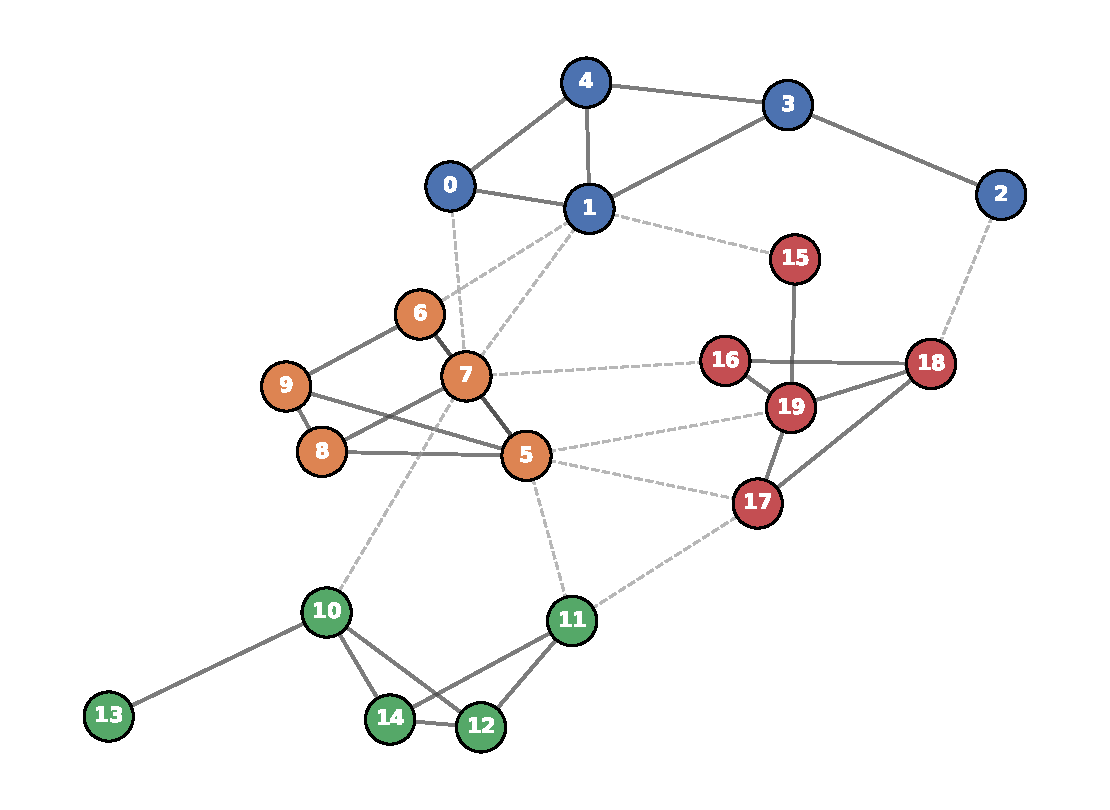
\includegraphics[width=0.78\textwidth]{partition_example.pdf}
    \caption[Ví dụ phân hoạch đồ thị $20$ đỉnh thành $4$ cụm.]{Ví dụ phân hoạch đồ thị $20$ đỉnh thành $4$ cụm. Cạnh liền nét là cạnh nội cụm, cạnh nét đứt là cạnh liên cụm.}
    \label{fig:partition-example}
\end{figure}

Đặc điểm quan trọng nhất khiến bài toán này khó là khái niệm cộng đồng vốn không có một định nghĩa toán học duy nhất. Trong mạng xã hội, cộng đồng có thể là một nhóm bạn bè thân thiết; trong mạng sinh học, có thể là một phức hợp protein cùng chức năng; trong mạng trích dẫn, có thể là một chủ đề nghiên cứu. Mỗi ngữ cảnh ứng với một tiêu chí khác nhau về ``thế nào là cộng đồng'', và do đó không có một phân hoạch nào được công nhận là đúng tuyệt đối cho mọi đồ thị. Để có thể đánh giá và so sánh các phân hoạch một cách có hệ thống, người ta đưa ra các tiêu chí đánh giá dưới dạng một hàm số 
\begin{equation}
    f: \mathcal{P}(V) \to \mathbb{R}
\end{equation}
\begin{itemize}
    \item Trong đó $\mathcal{P}(V)$ là tập tất cả các phân hoạch của $V$ thành các tập con không rỗng đôi một rời nhau.
\end{itemize}
Ngay cả khi đã cố định một tiêu chí $f$, việc tìm phân hoạch tối ưu $f$ vẫn là một bài toán khó. Lực lượng của $\mathcal{P}(V)$ tăng theo cấp số mũ với $n$, nên duyệt toàn bộ là không khả thi với đồ thị quy mô lớn. Hơn nữa, hai bài toán cụ thể là cực đại modularity và cực tiểu normalized cut đều thuộc lớp NP-khó \cite{newman2006, shi2000}.

% ............................................................
\subsection{Bài toán với modularity}
\label{subsec:problem-modularity}

\begin{definition}[Ma trận modularity]
\label{def:modularity-matrix}
Ma trận modularity được định nghĩa
\[
    B = A - \frac{d d^\top}{2m},
\]
trong đó $d \in \mathbb{R}^n$ là vector bậc của đồ thị.
\end{definition}

\begin{definition}[Modularity của phân hoạch \cite{newman2006}]
\label{def:modularity}

Cho phân hoạch của đồ thị $G$ là $\mathcal{C} = \{C_1, \ldots, C_K\}$ với $c_u$ ký hiệu cụm chứa đỉnh $u$, và $\delta(c_u, c_v)$ là Kronecker delta
\[
    \delta(c_u, c_v) = \begin{cases}
        1 & \text{nếu } c_u = c_v, \\
        0 & \text{nếu } c_u \neq c_v.
    \end{cases}
\]
Modularity được định nghĩa
\[
    Q(\mathcal{C}) = \frac{1}{2m} \sum_{u, v} \!\left( A_{uv} - \frac{d_u d_v}{2m} \right)\! \delta(c_u, c_v).
\]
Đặt $S \in \{0,1\}^{n \times K}$ là ma trận chỉ thị cụm với $S_{uk} = 1 \iff u \in C_k$. Khi đó
\[
    Q = \frac{1}{2m} \mathrm{Tr}(S^\top B S).
\]
\end{definition}

Ý nghĩa của $Q$ là chênh lệch giữa mật độ cạnh nội cụm thực tế và mật độ kỳ vọng. Giá trị $Q > 0$ nghĩa là phân hoạch tốt hơn ngẫu nhiên, $Q$ càng lớn càng phân hoạch tốt theo nghĩa cộng đồng.

\clearpage

\textbf{Bài toán phát hiện cộng đồng theo modularity} được phát biểu như sau. Hàm mục tiêu là vết của ma trận $S^\top B S$, đại diện cho modularity của một phân hoạch:
\begin{equation}
\label{eq:modularity-objective}
    \max_{S \in \mathbb{R}^{n \times K}} \; \mathrm{Tr}(S^\top B S).
\end{equation}
Trong đó, $S$ là ma trận nhãn thỏa mãn:

Mỗi phần tử $S_{uk}$ là nhãn cho biết đỉnh $u$ có thuộc cụm $k$ hay không, do đó chỉ nhận giá trị nhị phân:
\begin{equation}
\label{eq:mod-binary}
    S_{uk} \in \{0, 1\}, \qquad \forall\, u \in V,\ \forall\, k \in \{1, \ldots, K\}.
\end{equation}

Mỗi đỉnh thuộc đúng một cụm, tức là tổng các phần tử trên hàng tương ứng phải bằng $1$:
\begin{equation}
\label{eq:mod-row}
    \sum_{k=1}^K S_{uk} = 1, \qquad \forall\, u \in V.
\end{equation}

Không cụm nào được rỗng, tức là tổng các phần tử trên cột tương ứng phải lớn hơn hoặc bằng $1$:
\begin{equation}
\label{eq:mod-col}
    \sum_{u \in V} S_{uk} \geq 1, \qquad \forall\, k \in \{1, \ldots, K\}.
\end{equation}

Ba điều kiện trên trên tương đương với điều kiện $\mathcal{C} \in \mathcal{P}_K(V)$.

Bài toán \eqref{eq:modularity-objective} với các ràng buộc trên là NP-khó \cite{newman2006}. Phép nới lỏng phổ chuẩn thay các ràng buộc rời rạc bằng một ràng buộc trực giao đại số tuyến tính, biến bài toán tổ hợp thành bài toán liên tục giải được bằng phân tích trị riêng. Cơ sở của phép nới lỏng này là định lý Ky Fan, một tổng quát hóa của thương Rayleigh từ một vector lên $K$ vector trực giao.

\begin{theorem}[Tổng quát hóa Ky Fan \cite{kyfan1949}]
\label{thm:ky-fan}
Cho ma trận đối xứng $M \in \mathbb{R}^{n \times n}$ với các giá trị riêng $\lambda_1(M) \leq \cdots \leq \lambda_n(M)$ và các vector riêng đơn vị tương ứng $v_1, \ldots, v_n$. Khi đó với mọi $k \leq n$:
\[
    \max_{X \in \mathbb{R}^{n \times k},\ X^\top X = I_k} \mathrm{Tr}(X^\top M X) = \sum_{i=1}^k \lambda_{n-i+1}(M),
\]
\[
    \min_{X \in \mathbb{R}^{n \times k},\ X^\top X = I_k} \mathrm{Tr}(X^\top M X) = \sum_{i=1}^k \lambda_i(M).
\]
Nghiệm cực đại đạt tại $X^* = [v_n, v_{n-1}, \ldots, v_{n-k+1}]$ và nghiệm cực tiểu đạt tại $X^* = [v_1, v_2, \ldots, v_k]$.
\end{theorem}

Áp dụng định lý~\ref{thm:ky-fan} cho ma trận modularity $B$ với $k = K$, ta thay các ràng buộc rời rạc \eqref{eq:mod-binary}--\eqref{eq:mod-col} bằng ràng buộc trực giao $S^\top S = I_K$ và thu được bài toán liên tục
\begin{equation}
\label{eq:modularity-relaxed}
    \max_{S \in \mathbb{R}^{n \times K},\ S^\top S = I_K} \mathrm{Tr}(S^\top B S).
\end{equation}
Nghiệm tối ưu là $S^* = [v_n, v_{n-1}, \ldots, v_{n-K+1}]$ gồm $K$ vector riêng của $B$ ứng với $K$ giá trị riêng lớn nhất, và giá trị tối ưu bằng tổng $K$ giá trị riêng lớn nhất đó. Bước rời rạc hóa từ $S^* \in \mathbb{R}^{n \times K}$ về một phân hoạch cụ thể được thực hiện bằng $k$-means trên các hàng của $S^*$, sẽ trình bày ở Mục~\ref{sec:spectral-clustering}.

% ............................................................
\subsection{Bài toán với conductance}
\label{subsec:problem-conductance}

Chia tập đỉnh $V$ thành hai phần $V = S \cup \bar{S}$, trong đó $\emptyset \neq S \subsetneq V$ và $\bar{S} = V \setminus S$.

\begin{definition}[Cut và volume]
\label{def:cut-volume}
Cho $S \subset V$. Cut của $(S, \bar{S})$ là tổng trọng số các cạnh có một đầu trong $S$ và đầu kia trong $\bar{S}$:
\[
    \mathrm{cut}(S, \bar{S}) = \sum_{u \in S,\, v \in \bar{S}} A_{uv}.
\]
Volume của $S$ là tổng bậc các đỉnh trong $S$:
\[
    \mathrm{vol}(S) = \sum_{u \in S} d_u.
\]
\end{definition}

Chất lượng của nhát cắt $(S, \bar{S})$ được phản ánh trực tiếp bởi giá trị $\mathrm{cut}(S, \bar{S})$: giá trị càng nhỏ thì $S$ và $\bar{S}$ càng ít nối với nhau. Tuy nhiên dùng $\mathrm{cut}(S, \bar{S})$ làm tiêu chí có một nhược điểm cố hữu: các nhát cắt suy biến như $|S| = 1$ thường có giá trị $\mathrm{cut}$ rất nhỏ, tạo ra phân hoạch mất cân bằng. Để khắc phục, ta chuẩn hóa $\mathrm{cut}$ theo volume của mỗi phía, dẫn đến đại lượng conductance.

\begin{definition}[Conductance \cite{chung1997}]
\label{def:conductance}
Conductance của tập $S$ là
\[
    \phi(S) = \frac{\mathrm{cut}(S, \bar{S})}{\min(\mathrm{vol}(S), \mathrm{vol}(\bar{S}))}.
\]
Conductance tối thiểu của đồ thị là $\phi^* = \min_{\emptyset \neq S \subsetneq V} \phi(S)$.
\end{definition}

Mẫu số $\min(\mathrm{vol}(S), \mathrm{vol}(\bar{S}))$ ngăn các nhát cắt mất cân bằng đạt giá trị tối ưu một cách giả tạo. Bài toán cực tiểu hóa $\phi$ trên tất cả các nhát cắt là NP-khó, do đó cần một cách diễn giải khác để có thể tiếp cận bằng công cụ giải tích.

Quan sát then chốt là một nhát cắt $(S, \bar S)$ có thể biểu diễn bằng một hàm số gán giá trị cho từng đỉnh. Cụ thể, đặt $f: V \to \mathbb{R}$ là hàm chỉ thị của $S$,
\[
    f(u) = \begin{cases} 1 & \text{nếu } u \in S, \\ 0 & \text{nếu } u \in \bar{S}. \end{cases}
\]
Khi đó hai đại lượng cấu thành conductance đều biểu diễn được qua $f$. Số cạnh bị cắt bằng tổng bình phương sai phân của $f$ qua các cạnh:
\[
    \mathrm{cut}(S, \bar{S}) = \sum_{(u,v) \in E} \bigl( f(u) - f(v) \bigr)^2,
\]
vì $f(u) - f(v)$ bằng $\pm 1$ trên cạnh bị cắt và bằng $0$ trên cạnh không bị cắt. Tổng bình phương trên có thể hiểu là độ biến thiên của $f$ qua cấu trúc cạnh của đồ thị: $f$ thay đổi càng nhiều qua cạnh thì tổng càng lớn. Tương tự, volume của $S$ bằng tổng có trọng số bậc của các giá trị $f^2$:
\[
    \mathrm{vol}(S) = \sum_{u \in V} f(u)^2 \, d_u.
\]

Ý tưởng then chốt là tổng quát hóa: cho $f$ là hàm thực bất kỳ trên $V$, không nhất thiết nhị phân. Khi đó tỷ số
\[
    \mathcal{R}(f) = \frac{\sum_{(u,v) \in E} \bigl( f(u) - f(v) \bigr)^2}{\sum_{u \in V} f(u)^2 \, d_u}
\]
đo độ biến thiên của $f$ qua cạnh, chuẩn hóa theo độ lớn có trọng số của $f$. Khi $f$ là chỉ thị của $S$, ta có $\mathcal{R}(f) = \mathrm{cut}(S, \bar{S}) / \mathrm{vol}(S)$, gần với conductance về hình thức. Khi $f$ là hàm thực tổng quát, $\mathcal{R}(f)$ trở thành một bài toán liên tục có thể tối ưu bằng giải tích, đây chính là phép nới lỏng phổ của bài toán nhát cắt rời rạc. Tỷ số $\mathcal{R}(f)$ là dạng biến phân của thương Rayleigh trên đồ thị, được Chung phát biểu thành định nghĩa cơ bản trong lý thuyết phổ đồ thị \cite{chung1997}.

\begin{definition}[Thương Rayleigh trên đồ thị]
\label{def:rayleigh-graph}
Cho đồ thị có ma trận kề $A$, ma trận bậc $D$ và Laplacian không chuẩn hóa $L = D - A$. Với hàm $f: V \to \mathbb{R}$, $f \not\equiv 0$, thương Rayleigh của $f$ là
\[
    \mathcal{R}(f) = \frac{f^\top L f}{f^\top D f}
                  = \frac{\sum_{(u,v) \in E} \bigl( f(u) - f(v) \bigr)^2}{\sum_{u \in V} f(u)^2 \, d_u}.
\]
\end{definition}

Đẳng thức $f^\top L f = \sum_{(u,v) \in E} (f(u) - f(v))^2$ là đồng nhất thức cơ bản của Laplacian, nối dạng đại số ma trận với dạng biến phân trên đồ thị.

Đặt $g = D^{1/2} f$ và $\mathcal{L} = I - D^{-1/2} A D^{-1/2}$ là Laplacian chuẩn hóa, mẫu số trở thành $\|g\|^2$ và tử số trở thành $g^\top \mathcal{L} g$, do đó $\mathcal{R}(f) = R(\mathcal{L}, g)$ trong đó
\[
    R(M, x) = \frac{x^\top M x}{x^\top x}
\]
là thương Rayleigh đại số trên ma trận đối xứng $M$ tổng quát.

Nhờ đồng nhất thức trên, mọi câu hỏi về cực trị của $\mathcal{R}(f)$ đều quy về câu hỏi về phổ của $\mathcal{L}$. Quan sát rằng hàm hằng $f \equiv c$ cho $\mathcal{R}(f) = 0$ vì không có biến thiên qua cạnh nào, ứng với giá trị riêng nhỏ nhất $\lambda_1 = 0$ của $\mathcal{L}$. Khi loại bỏ thành phần hằng, cực tiểu của $\mathcal{R}(f)$ cho ta giá trị riêng nhỏ thứ hai. Kết quả tổng quát hơn cho mọi giá trị riêng được phát biểu qua định lý Courant--Fischer.

\begin{theorem}[{Tính chất biến phân Courant--Fischer \cite{horn2013}}]
\label{thm:courant-fischer}
Cho ma trận đối xứng $M \in \mathbb{R}^{n \times n}$ với các giá trị riêng $\lambda_1(M) \leq \cdots \leq \lambda_n(M)$ và các vector riêng đơn vị tương ứng $v_1, \ldots, v_n$. Khi đó với mọi $k \in \{1, \ldots, n\}$:
\[
    \lambda_k(M) = \min_{\substack{U \subset \mathbb{R}^n \\ \dim U = k}} \max_{x \in U \setminus \{0\}} R(M, x)
                 = \max_{x \perp v_1, \ldots, v_{k-1}} R(M, x).
\]
Đặc biệt, $\lambda_1(M) = \min_{x \neq 0} R(M, x)$ và $\lambda_n(M) = \max_{x \neq 0} R(M, x)$.
\end{theorem}

Áp dụng định lý~\ref{thm:courant-fischer} cho Laplacian chuẩn hóa $\mathcal{L}$ và phép biến đổi $g = D^{1/2} f$ ở trên, ta có
\[
    \lambda_2(\mathcal{L}) = \min_{f \perp d} \mathcal{R}(f),
\]
trong đó $f \perp d$ nghĩa là $\sum_u f(u) d_u = 0$, tức $f$ trực giao với vector bậc $d = D\mathbf{1}$. Đây là đáy của tỷ số biến thiên qua cạnh trên kích thước có trọng số khi đã loại bỏ thành phần hằng. Vì conductance được biểu diễn xấp xỉ qua $\mathcal{R}$ với hàm chỉ thị có trọng, $\lambda_2$ và $\phi^*$ phải có liên hệ định lượng với nhau. Liên hệ đó là nội dung của bất đẳng thức Cheeger.

\begin{theorem}[Bất đẳng thức Cheeger \cite{chung1997}]
\label{thm:cheeger}
Cho đồ thị vô hướng có trọng số không âm với ma trận kề $A$ và ma trận bậc $D = \mathrm{diag}(d_1, \ldots, d_n)$. Đặt
\[
    \mathcal{L} = I - D^{-1/2} A D^{-1/2}
\]
là Laplacian chuẩn hóa của đồ thị. Khi đó $\mathcal{L}$ đối xứng nửa xác định dương với các giá trị riêng
\[
    0 = \lambda_1 \leq \lambda_2 \leq \cdots \leq \lambda_n \leq 2,
\]
và conductance tối thiểu $\phi^*$ thỏa mãn cận hai phía
\[
    \frac{\lambda_2}{2} \;\leq\; \phi^* \;\leq\; \sqrt{2 \lambda_2}.
\]
\end{theorem}

Bất đẳng thức Cheeger kẹp $\phi^*$ giữa hai biểu thức của giá trị riêng $\lambda_2$, đại lượng còn được gọi là khoảng cách phổ của đồ thị. Cận dưới $\lambda_2 / 2 \leq \phi^*$ cho thấy không nhát cắt nào có conductance bé hơn $\lambda_2 / 2$, do đó $\lambda_2$ nhỏ là điều kiện cần để đồ thị có cộng đồng tách rõ. Cận trên $\phi^* \leq \sqrt{2 \lambda_2}$ là phần mang tính xây dựng: từ vector riêng ứng với $\lambda_2$, một thuật toán sweep cho phép tìm một nhát cắt cụ thể có conductance không vượt quá $\sqrt{2 \lambda_2}$. Hai cận này đảm bảo rằng cực tiểu hóa $\lambda_2$ trên các đồ thị có trọng số là một xấp xỉ chặt của bài toán cực tiểu hóa $\phi$.

Một điểm đáng lưu ý: bất đẳng thức Cheeger được phát biểu cho mọi đồ thị có trọng số không âm và đối xứng, không yêu cầu thêm điều kiện về cấu trúc. Tính tổng quát này sẽ đóng vai trò then chốt khi xét các biến thể đồ thị có trọng số ở Chương~\ref{chap:thuat-toan}.

\begin{definition}[Normalized Cut, Shi--Malik 2000 \cite{shi2000}]
\label{def:ncut}
Với phân hoạch hai cụm $\{S, \bar{S}\}$:
\[
    \mathrm{NCut}(S, \bar{S}) = \frac{\mathrm{cut}(S, \bar{S})}{\mathrm{vol}(S)} + \frac{\mathrm{cut}(S, \bar{S})}{\mathrm{vol}(\bar{S})}.
\]
Tổng quát hóa cho phân hoạch $K$ cụm:
\[
    \mathrm{NCut}(\mathcal{C}) = \sum_{k=1}^K \frac{\mathrm{cut}(C_k, \bar{C_k})}{\mathrm{vol}(C_k)}.
\]
\end{definition}

NCut là một dạng chuẩn hóa theo volume nên không bị thiên lệch về cụm rất nhỏ. Liên hệ với conductance: $\mathrm{NCut}(S, \bar{S}) \approx 2 \phi(S)$ khi hai cụm có volume xấp xỉ nhau.

\textbf{Bài toán tối ưu.} Bài toán phát hiện cộng đồng theo conductance hoặc theo normalized cut là
\[
    \mathcal{C}^*_{\mathrm{NCut}} = \arg\min_{\mathcal{C} \in \mathcal{P}_K(V)} \mathrm{NCut}(\mathcal{C}).
\]
Bài toán này là NP-khó \cite{shi2000}. Phép nới lỏng phổ tương ứng dẫn đến vector riêng nhỏ nhất của normalized Laplacian, được trình bày ở Mục~\ref{sec:spectral-clustering}.

% ============================================================
\section{Đồ thị Higher Order}
\label{sec:higher-order}

Mục~\ref{sec:problem} đã trình bày bài toán phát hiện cộng đồng dưới góc nhìn cạnh: chất lượng phân hoạch được đo qua conductance và modularity, đều là các đại lượng dựa trên cấu trúc cạnh đơn lẻ. Tuy nhiên trong nhiều mạng thực, đặc biệt là mạng xã hội, cấu trúc bậc cao mang theo tín hiệu cộng đồng mạnh hơn cả cạnh đơn lẻ. Mục này hình thức hóa khái niệm đó thông qua motif và đồ thị Higher Order, đồng thời chứng tỏ rằng tam giác $K_3$ là motif then chốt cho lớp đồ thị xã hội thực tế thông qua hệ số phân cụm.

% ............................................................
\subsection{Motif}
\label{subsec:motif}

\begin{definition}[Motif và motif instance]
\label{def:motif}
Motif $M$ là một đồ thị con nhỏ, cố định, được dùng làm đơn vị cấu trúc để phân tích đồ thị lớn. Một instance của $M$ trong $G = (V, E)$ là một đồ thị con của $G$ đẳng cấu với $M$.
\end{definition}

Việc chọn motif cụ thể nào phụ thuộc vào loại đồ thị đang xét, vì mỗi lớp đồ thị có cấu trúc bậc cao đặc trưng riêng. Phần bàn luận chi tiết về cách chọn motif sẽ được trình bày ở Mục~\ref{subsec:cc} sau khi giới thiệu hệ số phân cụm.

% ............................................................
\subsection{Hệ số phân cụm và vai trò của tam giác trong mạng xã hội}
\label{subsec:cc}

Để chứng tỏ một motif cụ thể mang ý nghĩa cộng đồng thực sự trong một lớp đồ thị nào đó, ta cần một đại lượng đo mật độ motif trên đồ thị, độc lập với phân hoạch cụ thể. Với motif là tam giác, đại lượng đó là hệ số phân cụm. 

Về mặt trực giác, hệ số phân cụm đặc trưng cho xác suất mà một bộ ba đỉnh đã có liên kết bộ phận thực sự khép lại thành một tam giác, và vì vậy phản ánh mức độ chặt chẽ trong cấu trúc kết nối của đồ thị: hệ số phân cụm càng cao, các đỉnh càng có xu hướng đan vào nhau thành các tam giác, một dấu hiệu cho thấy đồ thị mang cấu trúc cộng đồng đậm đặc hơn.

\begin{definition}[Hệ số phân cụm tại đỉnh]
\label{def:local-cc}
Hệ số phân cụm tại đỉnh $u$ là
\[
    cc(u) = \frac{2 \, T_u}{d_u (d_u - 1)},
\]
với $T_u$ là số tam giác chứa $u$ trong $G$. Quy ước $cc(u) := 0$ nếu $d_u \leq 1$.
\end{definition}

\begin{definition}[Hệ số phân cụm toàn cục]
\label{def:global-cc}
Một \emph{tam giác mở} tại đỉnh $v$ là một bộ ba có thứ tự $(u, v, w)$ với $u, w$ là hai hàng xóm phân biệt của $v$. Số tam giác mở của $G$ là
\[
    P_2 = \sum_{v \in V} d_v (d_v - 1).
\]
Hệ số phân cụm toàn cục của $G$ là
\[
    cc_{\mathrm{global}}(G) = \frac{6 T}{P_2} = \frac{6 T}{\sum_{v} d_v (d_v - 1)},
\]
với $T$ là tổng số tam giác trong $G$. Quy ước $cc_{\mathrm{global}}(G) := 0$ nếu $P_2 = 0$.
\end{definition}

Hệ số $cc_{\mathrm{global}}$ nhận giá trị trong $[0, 1]$ và đo xác suất một tam giác mở chọn ngẫu nhiên thực sự đóng thành tam giác. Khác với trung bình của $cc(u)$ trên các đỉnh, $cc_{\mathrm{global}}$ tính trọng số theo bậc đỉnh, do đó phản ánh đúng mật độ tam giác ở mức đồ thị mà không bị thiên lệch bởi các đỉnh bậc thấp. Trong khoá luận, $cc_{\mathrm{global}}$ được dùng làm tham chiếu để so sánh với hệ số phân cụm trên từng phân hoạch.

Đối với một phân hoạch $\mathcal{C} = \{C_1, \ldots, C_K\}$, hai đại lượng tổng hợp được dùng để đánh giá mức độ đóng kín tam giác trên các cụm.

\begin{definition}[Hệ số phân cụm trên phân hoạch]
\label{def:cc-cluster}
Cho cụm $C_j$ trong phân hoạch $\mathcal{C} = \{C_1, \ldots, C_K\}$, đặt
\[
    \mathrm{CC}(C_j) = \frac{1}{|C_j|} \sum_{u \in C_j} cc(u).
\]
Trung bình của các giá trị này trên các cụm với trọng số đều là
\[
    \overline{\mathrm{CC}}(\mathcal{C}) = \frac{1}{K} \sum_{j=1}^K \mathrm{CC}(C_j).
\]
\end{definition}

Đại lượng $\overline{\mathrm{CC}}(\mathcal{C})$ phản ánh mật độ tam giác trung bình bên trong mỗi cụm, nhưng bộc lộ một điểm yếu khi kích thước các cụm chênh lệch nhiều. Vì $\overline{\mathrm{CC}}$ gán đồng đều một lượng $\tfrac{1}{K}$ cho mọi cụm, một cụm chỉ gồm ba đỉnh nối thành $K_3$ luôn cho $\mathrm{CC} = 1$ và đóng góp ngang bằng một cụm hàng trăm hay hàng nghìn đỉnh. Hệ quả là một phân hoạch sinh ra nhiều cụm rất nhỏ với hệ số phân cụm cao có thể đạt $\overline{\mathrm{CC}}$ gần $1$ mặc dù về mặt cấu trúc cộng đồng, các cụm cỡ ba đỉnh thường không mang ý nghĩa thực sự. Để khắc phục điểm yếu này, thay vì gán trọng số đều cho các cụm, ta gán trọng số tỉ lệ với kích thước cụm, dẫn tới đại lượng sau đây.

\begin{definition}[Hệ số phân cụm có trọng số]
\label{def:cc-weighted}
Hệ số phân cụm có trọng số của phân hoạch $\mathcal{C} = \{C_1, \ldots, C_K\}$ là trung bình có trọng số tỉ lệ với kích thước cụm:
\[
    \overline{\mathrm{CC}}_w(\mathcal{C})
        = \frac{\sum_{j=1}^K |C_j| \, \mathrm{CC}(C_j)}{\sum_{j=1}^K |C_j|}
        = \frac{1}{n} \sum_{u \in V} cc(u).
\]
\end{definition}

Trong $\overline{\mathrm{CC}}_w$, mỗi cụm đóng góp theo đúng số đỉnh nó chứa, nên cụm $K_3$ chỉ đóng góp ba đỉnh trên tổng $n$, không thể kéo trung bình lên cao chỉ vì có $\mathrm{CC} = 1$. Công thức rút gọn $\overline{\mathrm{CC}}_w(\mathcal{C}) = \tfrac{1}{n}\sum_{u} cc(u)$ cho thấy đại lượng này thực chất là trung bình hệ số phân cụm tại đỉnh trên toàn bộ đồ thị, không phụ thuộc cách phân hoạch chia cụm. Vì lý do đó, $\overline{\mathrm{CC}}_w$ được dùng làm đại lượng đánh giá chính trong khoá luận; $\overline{\mathrm{CC}}$ được tính kèm để phát hiện hiện tượng phân hoạch tạo ra cụm rất nhỏ làm thiên lệch chỉ số.

\textbf{Bằng chứng thống kê cho vai trò của tam giác.} Việc chọn tam giác $K_3$ làm motif không phải lựa chọn tùy ý mà được công nhận rộng rãi trong tài liệu phân tích mạng nhờ bằng chứng thống kê trên nhiều lớp mạng thực tế khác nhau. Watts và Strogatz \cite{watts1998} là những người đầu tiên chỉ ra rằng nhiều mạng thực, từ mạng diễn viên đồng diễn, mạng kết nối synapse trong hệ thần kinh của giun \emph{C. elegans} đến mạng lưới điện, có hệ số phân cụm trung bình lớn hơn rất nhiều so với mô hình ngẫu nhiên có cùng số đỉnh và cạnh. Kết quả này được Newman tổng hợp lại trong khảo sát \cite{newman2003structure} cho nhiều lớp mạng thực: mạng cộng tác khoa học, mạng email, mạng web, mạng xã hội. Hệ số phân cụm trung bình trên các mạng này nằm trong khoảng $0{,}1$--$0{,}8$, trong khi mật độ cạnh thường chỉ ở mức $10^{-3}$ trở xuống. Hai đại lượng này có thể so sánh trực tiếp vì cùng thang đo: $cc(u)$ là xác suất có điều kiện rằng hai hàng xóm của $u$ nối với nhau, còn mật độ cạnh là xác suất hai đỉnh bất kỳ nối với nhau. Trên đồ thị ngẫu nhiên Erdős--Rényi $G(n, p)$ với các cạnh độc lập, hai xác suất này bằng nhau và đều bằng $p$. Trên các mạng thực kể trên, $cc$ lớn hơn mật độ cạnh từ một đến nhiều bậc.

Nếu các cạnh được sinh độc lập với nhau như trong mô hình Erdős--Rényi, kỳ vọng của $cc(u)$ chính bằng mật độ cạnh, do đó khoảng cách giữa hai con số trên không thể giải thích bằng hiệu ứng ngẫu nhiên. Cơ chế tạo nên khoảng cách này là triadic closure, một quy luật xã hội đã được nghiên cứu từ sớm bởi Granovetter \cite{granovetter1973} và Holland--Leinhardt \cite{holland1971}: hai đỉnh chia sẻ hàng xóm có xu hướng kết nối với nhau cao hơn nhiều so với cặp đỉnh ngẫu nhiên. Mật độ tam giác cao hơn dự đoán ngẫu nhiên do đó là tín hiệu cộng đồng đáng tin cậy chứ không phải nhiễu ngẫu nhiên.


% ............................................................
\subsection{Đồ thị Higher Order}
\label{subsec:higher-order-graph}

Ý tưởng đưa cấu trúc bậc cao vào bài toán phân cụm được hình thức hóa qua việc xây dựng một đồ thị mới trên cùng tập đỉnh của $G$, trong đó trọng số cạnh giữa hai đỉnh phản ánh số motif chứa cả hai. Đồ thị mới này được gọi là đồ thị Higher Order.

\begin{definition}[Ma trận motif và đồ thị Higher Order]
\label{def:motif-matrix}
Cho đồ thị $G = (V, E)$ và motif $M$. Ma trận motif của $G$ ứng với $M$ là $W^{(M)} \in \mathbb{R}^{n \times n}$ với
\[
    W^{(M)}_{uv} = \bigl| \{\, \text{instance của } M \text{ chứa cả } u \text{ và } v \,\} \bigr|.
\]
Đồ thị Higher Order $G_M = (V, W^{(M)})$ là đồ thị có trọng số trên cùng tập đỉnh $V$, với ma trận trọng số $W^{(M)}$.
\end{definition}

Phép xây dựng nói trên có một diễn giải tự nhiên trên mạng xã hội: hai người cùng tham gia một tam giác bạn bè được kết nối qua hai con đường, một cạnh trực tiếp và một con đường gián tiếp qua người thứ ba. Mỗi tam giác mà cả hai cùng thuộc về làm tăng cường mức độ gần gũi của họ. Đồ thị Higher Order $G_M$ định lượng mức độ gần gũi đó bằng cách đặt trọng số cạnh giữa hai đỉnh đúng bằng số motif chứa cả hai.

Hình~\ref{fig:higher-order-construction} minh họa phép xây dựng này trên một đồ thị mẫu nhỏ.

\begin{figure}[H]
    \centering
    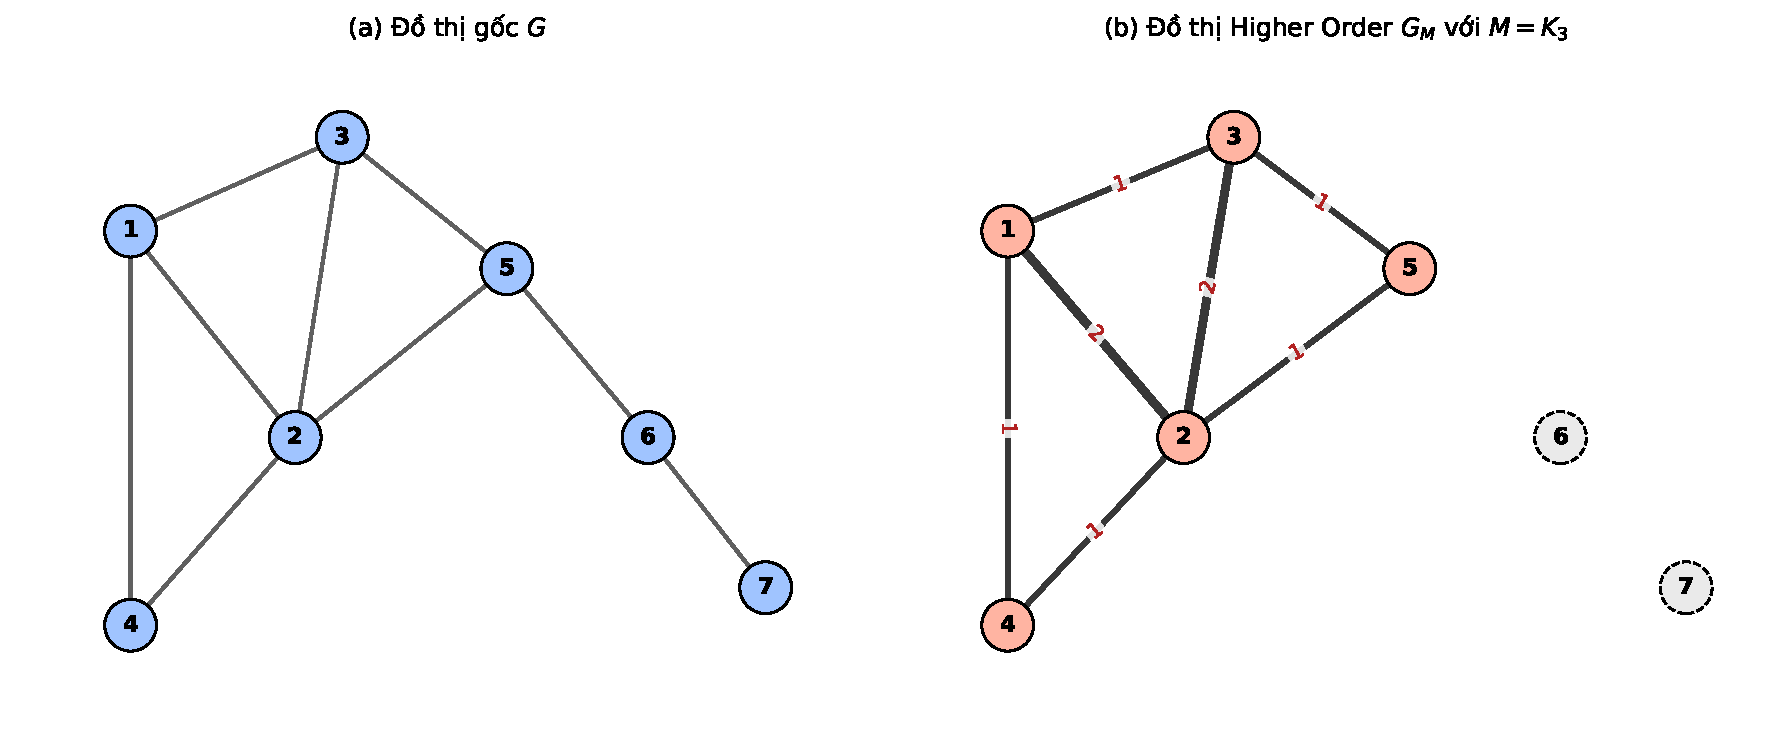
\includegraphics[width=\textwidth]{higher_order_construction.pdf}
    \caption[Xây dựng đồ thị Higher Order $G_M$ từ đồ thị gốc $G$ với $M = K_3$.]{Xây dựng đồ thị Higher Order $G_M$ từ đồ thị gốc $G$ với $M = K_3$. Ở (b), trọng số mỗi cạnh bằng số tam giác chứa cả hai đỉnh, các cạnh không thuộc tam giác nào trong $G$ bị loại bỏ, các đỉnh không thuộc tam giác nào trở thành cô lập (vẽ với viền đứt nét).}
    \label{fig:higher-order-construction}
\end{figure}

\begin{theorem}[Higher-order Cheeger inequality \cite{benson2016}]
\label{thm:higher-cheeger}
\label{prop:gm-valid-weighted-graph}
Ma trận $W^{(M)}$ đối xứng và không âm, nên $G_M = (V, W^{(M)})$ là đồ thị có trọng số vô hướng hợp lệ. Tương tự đồ thị gốc, đặt motif degree $d_u^{(M)} = \sum_{v \in V} W^{(M)}_{uv}$, motif volume $\mathrm{vol}_M(S) = \sum_{u \in S} d_u^{(M)}$, đại lượng cắt theo motif
\[
    \mathrm{cut}_M(S, \bar{S}) = \bigl| \{\, \text{motif instance có ít nhất một đỉnh ở mỗi bên} \,\} \bigr|,
\]
và conductance motif tương ứng
\[
    \phi_M(S) = \frac{\mathrm{cut}_M(S, \bar{S})}{\min(\mathrm{vol}_M(S), \mathrm{vol}_M(\bar{S}))}.
\]
Khi đó mọi kết quả phổ phát biểu cho lớp đồ thị có trọng số áp dụng nguyên dạng cho $G_M$, bao gồm bất đẳng thức Cheeger và các phép nới lỏng phổ của NCut hay modularity. Cụ thể, phân cụm phổ trên $W^{(M)}$ thu được nhát cắt có $\phi_M$ gần tối ưu, với cùng dạng cận như bất đẳng thức Cheeger cổ điển.
\end{theorem}

\begin{remark}[Hai hạn chế của $G_M$ thuần]
\label{rem:gm-limit}
\leavevmode
\begin{enumerate}[topsep=4pt, itemsep=4pt, parsep=0pt]
    \item $G_M$ có thể không liên thông: đỉnh không thuộc bất kỳ instance nào của $M$ sẽ bị cô lập trong $G_M$, dù trong $G$ gốc có thể có nhiều cạnh kề.
    \item $G_M$ mất thông tin cạnh gốc: cạnh không thuộc instance nào của $M$ bị xóa hoàn toàn trong $G_M$, dù có thể mang thông tin cộng đồng quan trọng.
\end{enumerate}
\end{remark}

Hai hạn chế trên có thể quan sát trực tiếp trên Hình~\ref{fig:higher-order-construction}. Chúng là động lực trực tiếp cho cách tiếp cận đề xuất ở Chương~\ref{chap:thuat-toan}.

\textbf{Cố định motif $M = K_3$ cho phần còn lại của khóa luận.} Định nghĩa~\ref{def:motif-matrix} cho phép $M$ là một motif tùy ý, mở ra nhiều cấu trúc bậc cao khác nhau. Trên cơ sở bằng chứng thống kê đã trình bày ở Mục~\ref{subsec:cc}, cộng với các ưu điểm thuật toán, khóa luận cố định motif là tam giác trong toàn bộ phần còn lại với ba lý do:
\leavevmode
\begin{enumerate}[topsep=4pt, itemsep=4pt, parsep=0pt]
    \item Tam giác xuất hiện trong mạng xã hội thực tế với mật độ vượt xa kỳ vọng ngẫu nhiên, được giải thích bởi triadic closure, do đó mang tín hiệu cộng đồng có ý nghĩa.
    \item Số tam giác chứa từng đỉnh hoặc từng cạnh trong đồ thị thưa có thể đếm hiệu quả với độ phức tạp $O(m^{3/2})$, không trở thành bottleneck cho thuật toán quy mô lớn.
    \item Tam giác đối xứng tự nhiên trên ba đỉnh, không yêu cầu xử lý hướng cạnh hay vai trò không đối xứng giữa các đỉnh, làm cho ma trận motif $W^{(M)}$ đơn giản nhất có thể trong lớp các motif kích thước lớn hơn hai.
\end{enumerate}
Việc khảo sát các motif khác như $K_4$ hay bi-fan là một hướng mở rộng tự nhiên, nhưng nằm ngoài phạm vi của khóa luận này.

% ============================================================
\section{Thuật toán phân cụm phổ}
\label{sec:spectral-clustering}

Trên các lớp đồ thị đã được định nghĩa, gồm đồ thị gốc $G$ và đồ thị Higher Order $G_M$, phân cụm phổ là một trong những thuật toán ứng dụng tốt nhất phép tọa độ hóa qua phổ của Laplacian, và đã được chứng minh là cách hiệu quả để tối ưu normalized cut trên đồ thị có trọng số không âm \cite{shi2000}.

% ............................................................
\subsection{Thuật toán $K$-means}
\label{subsec:kmeans}

Thuật toán $K$-means được trình bày tổng quát cho tập $n$ điểm trong $\mathbb{R}^d$ với số chiều $d$ tùy ý. Thuật toán cực tiểu hóa tổng bình phương khoảng cách từ mỗi điểm đến tâm cụm chứa nó qua hai bước lặp xen kẽ: gán điểm về tâm gần nhất và cập nhật tâm thành trung bình của cụm.

\begin{algorithm}[H]
\caption{Thuật toán $K$-means}
\label{alg:kmeans}
\KwIn{Tập điểm $X = \{x_1, \ldots, x_n\} \subset \mathbb{R}^d$; số cụm $K$.}
\KwOut{Phân hoạch $\{C_1, \ldots, C_K\}$ và tâm $\{\mu_1, \ldots, \mu_K\}$.}
Khởi tạo $K$ tâm $\mu_1, \ldots, \mu_K$ là $K$ điểm ngẫu nhiên trong không gian\;
\Repeat{phân hoạch không thay đổi}{
    \textbf{Bước gán:} với mỗi $x_i$, đặt $C_{k}$ là cụm có tâm gần nhất, $k = \arg\min_j \|x_i - \mu_j\|$\;
    \textbf{Bước cập nhật:} đặt $\mu_k \gets \frac{1}{|C_k|} \sum_{x \in C_k} x$ với mỗi $k$\;
}
\end{algorithm}

Đặt hàm mục tiêu
\[
    J\bigl(\{C_k\}, \{\mu_k\}\bigr) = \sum_{k=1}^K \sum_{x \in C_k} \|x - \mu_k\|^2.
\]

\iffalse
\begin{theorem}[Tính hội tụ của thuật toán $K$-means]
\label{thm:kmeans-convergence}
Dãy giá trị $J$ sinh bởi Thuật toán~\ref{alg:kmeans} đơn điệu không tăng và dừng sau hữu hạn bước tại một cực tiểu địa phương của $J$.
\end{theorem}

\begin{proof}
Ký hiệu $\bigl(\{C_k^{(t)}\}, \{\mu_k^{(t)}\}\bigr)$ là trạng thái sau vòng lặp thứ $t$, với quy ước $\{\mu_k^{(0)}\}$ là tập tâm khởi tạo. Mỗi vòng lặp $t \to t+1$ gồm hai bước: bước gán sinh phân hoạch mới $\{C_k^{(t+1)}\}$ từ tâm $\{\mu_k^{(t)}\}$, sau đó bước cập nhật sinh tâm mới $\{\mu_k^{(t+1)}\}$ từ phân hoạch $\{C_k^{(t+1)}\}$. Ta chứng minh
\[
    J\bigl(\{C_k^{(t+1)}\}, \{\mu_k^{(t+1)}\}\bigr) \;\leq\; J\bigl(\{C_k^{(t+1)}\}, \{\mu_k^{(t)}\}\bigr) \;\leq\; J\bigl(\{C_k^{(t)}\}, \{\mu_k^{(t)}\}\bigr).
\]

\emph{Bất đẳng thức thứ hai (bước gán).} Với mỗi $x \in X$, ký hiệu $c^{(t)}(x) \in \{1, \ldots, K\}$ là chỉ số cụm chứa $x$ ở vòng lặp $t$. Bằng cách hoán đổi thứ tự lấy tổng, hàm mục tiêu viết lại dưới dạng tổng theo điểm:
\[
    J\bigl(\{C_k^{(t)}\}, \{\mu_k^{(t)}\}\bigr) \;=\; \sum_{k=1}^K \sum_{x \in C_k^{(t)}} \|x - \mu_k^{(t)}\|^2 \;=\; \sum_{x \in X} \|x - \mu_{c^{(t)}(x)}^{(t)}\|^2,
\]
và tương tự cho trạng thái $(t+1)$ với tâm vẫn là $\{\mu_k^{(t)}\}$:
\[
    J\bigl(\{C_k^{(t+1)}\}, \{\mu_k^{(t)}\}\bigr) \;=\; \sum_{x \in X} \|x - \mu_{c^{(t+1)}(x)}^{(t)}\|^2.
\]
Theo định nghĩa của bước gán,
\[
    c^{(t+1)}(x) \;=\; \arg\min_{k \in \{1, \ldots, K\}} \|x - \mu_k^{(t)}\|^2,
\]
nên với mọi $x \in X$, $\|x - \mu_{c^{(t+1)}(x)}^{(t)}\|^2 \leq \|x - \mu_{c^{(t)}(x)}^{(t)}\|^2$. Cộng theo $x$ thu được bất đẳng thức thứ hai.

\emph{Bất đẳng thức thứ nhất (bước cập nhật).} Cố định phân hoạch $\{C_k^{(t+1)}\}$, hàm mục tiêu là tổng theo cụm của các hàm độc lập theo $\mu_k$:
\[
    J\bigl(\{C_k^{(t+1)}\}, \{\mu_k\}\bigr) \;=\; \sum_{k=1}^K h_k(\mu_k), \quad \text{với } h_k(\mu) := \sum_{x \in C_k^{(t+1)}} \|x - \mu\|^2.
\]
Cực tiểu hoá vế trái theo $\{\mu_k\}$ quy về cực tiểu hoá độc lập từng $h_k$. Đặt $\bar{x}_k = \frac{1}{|C_k^{(t+1)}|} \sum_{x \in C_k^{(t+1)}} x$ là trung bình cụm. Khai triển bình phương quanh $\bar{x}_k$ và viết $x - \mu = (x - \bar{x}_k) - (\mu - \bar{x}_k)$:
\begin{align*}
    h_k(\mu) &= \sum_{x \in C_k^{(t+1)}} \bigl\|(x - \bar{x}_k) - (\mu - \bar{x}_k)\bigr\|^2 \\
             &= \sum_{x \in C_k^{(t+1)}} \|x - \bar{x}_k\|^2 - 2 \Bigl\langle \mu - \bar{x}_k,\, \sum_{x \in C_k^{(t+1)}} (x - \bar{x}_k) \Bigr\rangle \\
             &\quad + |C_k^{(t+1)}| \, \|\mu - \bar{x}_k\|^2.
\end{align*}
Số hạng giữa triệt tiêu vì $\sum_{x \in C_k^{(t+1)}} (x - \bar{x}_k) = 0$ theo định nghĩa của $\bar{x}_k$, do đó
\[
    h_k(\mu) \;=\; \underbrace{\sum_{x \in C_k^{(t+1)}} \|x - \bar{x}_k\|^2}_{\text{hằng số theo } \mu} \;+\; |C_k^{(t+1)}| \, \|\mu - \bar{x}_k\|^2.
\]
Vế phải đạt cực tiểu duy nhất tại $\mu = \bar{x}_k$ vì $|C_k^{(t+1)}| > 0$ và $\|\mu - \bar{x}_k\|^2 \geq 0$ với dấu bằng khi và chỉ khi $\mu = \bar{x}_k$. Bước cập nhật đặt $\mu_k^{(t+1)} = \bar{x}_k$ cho mọi $k$, do đó $h_k(\mu_k^{(t+1)}) \leq h_k(\mu_k^{(t)})$. Cộng theo $k$ và áp dụng đẳng thức tổng theo cụm ở trên:
\begin{align*}
    J\bigl(\{C_k^{(t+1)}\}, \{\mu_k^{(t+1)}\}\bigr)
        &= \sum_{k=1}^K h_k(\mu_k^{(t+1)}) \\
        &\leq \sum_{k=1}^K h_k(\mu_k^{(t)})
         = J\bigl(\{C_k^{(t+1)}\}, \{\mu_k^{(t)}\}\bigr),
\end{align*}
chính là bất đẳng thức thứ nhất.

\emph{Dừng sau hữu hạn bước.} Hai bất đẳng thức trên kéo theo dãy $\{J^{(t)}\}$ với $J^{(t)} = J\bigl(\{C_k^{(t)}\}, \{\mu_k^{(t)}\}\bigr)$ đơn điệu không tăng và bị chặn dưới bởi $0$. Sau bước cập nhật, $\{\mu_k^{(t)}\}$ hoàn toàn xác định bởi $\{C_k^{(t)}\}$ (là trung bình các cụm), nên trạng thái $(\{C_k^{(t)}\}, \{\mu_k^{(t)}\})$ với $t \geq 1$ chỉ phụ thuộc vào phân hoạch $\{C_k^{(t)}\}$. Số phân hoạch của $X$ thành $K$ cụm hữu hạn, nên dãy $\{J^{(t)}\}$ chỉ nhận hữu hạn giá trị phân biệt. Giả sử dãy không dừng sau hữu hạn bước, nghĩa là tồn tại hai chỉ số $t_1 < t_2$ với $\{C_k^{(t_1)}\} = \{C_k^{(t_2)}\}$. Khi đó $J^{(t_1)} = J^{(t_2)}$ và do tính không tăng, $J^{(t)} = J^{(t_1)}$ với mọi $t \in [t_1, t_2]$. Mỗi vòng lặp $t \to t+1$ trong đoạn này không làm giảm $J$ và do đó cả hai bất đẳng thức trên đều là đẳng thức. Đẳng thức trong bước cập nhật buộc $\mu_k^{(t+1)} = \mu_k^{(t)}$ cho mọi $k$ (do cực tiểu duy nhất của $h_k$). Đẳng thức trong bước gán cùng với tính không đổi của tâm buộc $\{C_k^{(t+1)}\} = \{C_k^{(t)}\}$ với quy tắc phá tie nhất quán. Điều kiện dừng trong Thuật toán~\ref{alg:kmeans} (phân hoạch không đổi) được thoả mãn ngay tại bước $t_1$, mâu thuẫn với giả thiết dãy không dừng.

\emph{Tính chất điểm dừng.} Trạng thái dừng $(\{C_k\}, \{\mu_k\})$ thoả hai điều kiện cực tiểu theo từng nhóm biến: $\{C_k\}$ là cực tiểu của $J(\cdot, \{\mu_k\})$ trên không gian phân hoạch (bước gán), và $\{\mu_k\}$ là cực tiểu của $J(\{C_k\}, \cdot)$ trên $\mathbb{R}^{d \times K}$ (bước cập nhật). Đây là điểm dừng theo phép giảm toạ độ, thường được gọi là cực tiểu địa phương của $J$ trong tài liệu chuẩn.
\end{proof}

\begin{corollary}
\label{cor:kmeans-init}
Nghiệm trả về bởi Thuật toán~\ref{alg:kmeans} phụ thuộc vào vị trí của $K$ tâm khởi tạo, và không có bảo đảm trùng với cực tiểu toàn cục của $J$.
\end{corollary}

Hệ quả~\ref{cor:kmeans-init} là hệ quả trực tiếp của Định lý~\ref{thm:kmeans-convergence}: thuật toán chỉ đảm bảo dừng tại cực tiểu địa phương, mà $J$ thường có nhiều cực tiểu địa phương khác nhau ứng với các phân hoạch khác nhau. Hai lần chạy với $K$ điểm ngẫu nhiên khác nhau có thể rơi vào hai bể hấp dẫn khác nhau, cho hai nghiệm khác nhau. Trong thực hành, thuật toán được chạy nhiều lần với các khởi tạo ngẫu nhiên độc lập, và kết quả có $J$ nhỏ nhất được giữ lại làm nghiệm.
\fi

Thuật toán $K$-means có thể được hiểu là một dạng phép giảm toạ độ trên hàm mục tiêu $J$: bước gán cực tiểu $J$ với $\{\mu_k\}$ cố định, bước cập nhật cực tiểu $J$ với $\{C_k\}$ cố định. Do đó $J$ không tăng qua mỗi vòng lặp, bị chặn dưới bởi $0$ và chỉ nhận hữu hạn giá trị vì số phân hoạch của $X$ thành $K$ cụm là hữu hạn, nên thuật toán dừng sau hữu hạn bước. Điểm dừng phụ thuộc vào tâm khởi tạo và không nhất thiết là cực tiểu toàn cục của $J$, nên trong thực hành thuật toán được chạy nhiều lần với khởi tạo ngẫu nhiên độc lập và lấy nghiệm có $J$ nhỏ nhất.

% ............................................................
\subsection{Tọa độ hóa các đỉnh bằng phổ của toán tử Laplace}
\label{subsec:spectral-embedding}

Cho ma trận trọng số $W$ đối xứng không âm trên $V$, ma trận bậc $D = \mathrm{diag}(W \mathbf{1})$ và Laplacian chuẩn hóa $\mathcal{L} = I - D^{-1/2} W D^{-1/2}$. Theo Định lý~\ref{thm:cheeger}, $\mathcal{L}$ đối xứng nửa xác định dương với phổ $0 = \lambda_1 \leq \lambda_2 \leq \cdots \leq \lambda_n \leq 2$ và hệ vector riêng đơn vị $u_1, \ldots, u_n$ trực giao đôi một.

\begin{definition}[Tọa độ phổ của đỉnh \cite{belkin2003}]
\label{def:spectral-embedding}
Đặt $U = [u_1, u_2, \ldots, u_K] \in \mathbb{R}^{n \times K}$ là ma trận có cột là $K$ vector riêng đầu của $\mathcal{L}$. Tọa độ phổ $K$ chiều của đỉnh là ánh xạ $\psi: V \to \mathbb{R}^K$ gán cho mỗi đỉnh $u$ hàng thứ $u$ của $U$:
\[
    \psi(u) = \bigl( u_1(u), u_2(u), \ldots, u_K(u) \bigr).
\]
\end{definition}

Trực giác cho phép tọa độ hóa này được Chung \cite{chung1997} trình bày qua trường hợp $K = 2$. Vector riêng $u_2$ ứng với giá trị riêng nhỏ thứ hai của $\mathcal{L}$ chia tập đỉnh thành hai nhóm theo dấu của tọa độ: đỉnh có $u_2(u) > 0$ thuộc một cộng đồng, đỉnh có $u_2(u) < 0$ thuộc cộng đồng còn lại. Quan sát then chốt là các đỉnh trong cùng một cộng đồng có xu hướng nhận giá trị tương tự nhau trên $u_2$, vì $u_2$ tối thiểu hóa tổng bình phương sai phân qua các cạnh: hai đỉnh nối với nhau bằng một cạnh thường có giá trị $u_2$ gần nhau. Cộng đồng được hiểu là tập đỉnh nối nhau dày đặc, do đó các đỉnh bên trong một cộng đồng bị ràng buộc nhận giá trị $u_2$ gần nhau, còn hai cộng đồng khác nhau ngăn cách bởi ít cạnh hơn nên có thể nhận giá trị $u_2$ lệch dấu.

Trường hợp $K$ cộng đồng được Shi và Malik \cite{shi2000} tổng quát hóa trực tiếp: thay vì một tọa độ duy nhất, mỗi đỉnh được mô tả bằng $K$ tọa độ ứng với $K$ vector riêng đầu. Hai đỉnh cùng cộng đồng có $K$ tọa độ tương tự nhau, do đó $\psi(u)$ và $\psi(v)$ gần nhau theo khoảng cách Euclidean. Hai đỉnh khác cộng đồng được phân biệt bởi ít nhất một trong $K$ vector riêng, nên $\psi(u)$ và $\psi(v)$ cách xa nhau. Bài toán tìm cộng đồng trong $G$ do đó trở thành bài toán phân cụm $\{\psi(u)\}_{u \in V}$ trong không gian Euclidean $\mathbb{R}^K$, áp dụng được Thuật toán~\ref{alg:kmeans}.

% ............................................................
\subsection{Thuật toán phân cụm phổ chuẩn hóa}
\label{subsec:full-algorithm}

Gộp hai bước trên ta được thuật toán phân cụm phổ chuẩn hóa, áp dụng cho ma trận trọng số đối xứng không âm bất kỳ.

\begin{algorithm}[H]
\caption{Phân cụm phổ chuẩn hóa cho $K$ cụm}
\label{alg:spectral-clustering}
\KwIn{Ma trận trọng số $W$ đối xứng không âm trên $n$ đỉnh; số cụm $K$.}
\KwOut{Phân hoạch $\mathcal{C} = \{C_1, \ldots, C_K\}$ của $V$.}
$D \gets \mathrm{diag}(W \mathbf{1})$\;
$\mathcal{L} \gets I - D^{-1/2} W D^{-1/2}$\;
Tính $u_1, \ldots, u_K$: $K$ vector riêng nhỏ nhất của $\mathcal{L}$\;
Đặt $U \gets [u_1, \ldots, u_K] \in \mathbb{R}^{n \times K}$\;
Chuẩn hóa từng hàng của $U$ về độ dài đơn vị, thu được $\widetilde U$\;
Đặt $\psi(u) \gets \widetilde U_{u, :}$ với mỗi đỉnh $u$\;
Chạy Thuật toán~\ref{alg:kmeans} trên tập $\{\psi(u)\}_{u \in V}$ với $K$ cụm\;
\Return phân hoạch tương ứng của $V$\;
\end{algorithm}

Độ phức tạp tính toán gồm hai phần. Bước phân tích phổ tính $K$ vector riêng đầu của $\mathcal{L}$ tốn $O(K n m)$ với phương pháp Lanczos thưa khi $W$ thưa, hoặc $O(n^3)$ với phân tích đầy đủ. Bước $k$-means tốn $O(t K n)$ với $t$ là số vòng lặp, thường nhỏ trong thực hành. Tổng độ phức tạp do đó bị chi phối bởi bước phân tích phổ.

Trong khóa luận, Thuật toán~\ref{alg:spectral-clustering} được áp dụng với ba lựa chọn $W$ khác nhau: $W = A$ cho phân cụm phổ cổ điển trên đồ thị gốc, $W = W^{(M)}$ cho phân cụm trên đồ thị Higher Order, và $W = W_\lambda = A + \lambda W^{(M)}$ cho phương pháp đề xuất ở Chương~\ref{chap:thuat-toan}. Cả ba lựa chọn đều cho ma trận đối xứng không âm, do đó áp dụng được trực tiếp.

% ............................................................
\subsection{Đánh giá và tính đúng đắn}
\label{subsec:correctness}

Mục này trình bày tính đúng đắn của Thuật toán~\ref{alg:spectral-clustering} theo nghĩa: nghiệm thu được là một xấp xỉ định lượng của conductance tối ưu $\phi^*$. Khung chứng minh được Chung trình bày trong sách \cite{chung1997}, đi từ trường hợp $K = 2$ qua phép sweep trên vector Fiedler, sau đó tổng quát hóa lên $K$ cụm.

\emph{Trường hợp $K = 2$.} Thuật toán~\ref{alg:spectral-clustering} với $K = 2$ thực chất tương đương với phép sweep trên vector Fiedler $u_2$: sắp xếp các đỉnh theo giá trị của $u_2$ và xét tất cả các nhát cắt prefix, chọn nhát cắt có conductance nhỏ nhất. Gọi $S^{\mathrm{sweep}}$ là nhát cắt thu được.

\begin{theorem}[Cận sweep \cite{chung1997}]
\label{thm:sweep-bound}
Nhát cắt $S^{\mathrm{sweep}}$ thỏa
\[
    \phi(S^{\mathrm{sweep}}) \;\leq\; \sqrt{2 \lambda_2}.
\]
\end{theorem}

Kết hợp Định lý~\ref{thm:sweep-bound} với cận dưới của bất đẳng thức Cheeger, $\lambda_2 / 2 \leq \phi^*$ (Định lý~\ref{thm:cheeger}), ta thu được
\[
    \phi^* \;\leq\; \phi(S^{\mathrm{sweep}}) \;\leq\; \sqrt{2 \lambda_2} \;\leq\; 2 \sqrt{\phi^*}.
\]
Bất đẳng thức kép này là kết quả mấu chốt: nghiệm $S^{\mathrm{sweep}}$ của thuật toán phổ luôn nằm trong khoảng hằng số nhân với $\sqrt{\phi^*}$ so với nghiệm tối ưu. Khi $\phi^*$ nhỏ, tức đồ thị có cộng đồng tách rõ, $\phi(S^{\mathrm{sweep}})$ cũng nhỏ và nghiệm phổ gần tối ưu.

\emph{Trường hợp $K$ cụm.} Khi $K > 2$, định nghĩa hằng số Cheeger bậc cao $\rho_K(G) = \min_{\mathcal{C}} \max_k \phi(C_k)$, lấy tối thiểu trên các phân hoạch $\mathcal{C}$ thành $K$ cụm. Lee, Oveis Gharan và Trevisan tổng quát hóa bất đẳng thức Cheeger thành
\[
    \frac{\lambda_K}{2} \;\leq\; \rho_K(G) \;\leq\; O(K^2) \sqrt{\lambda_K},
\]
trong đó cận trên đạt được một cách xây dựng thông qua Thuật toán~\ref{alg:spectral-clustering}: phân hoạch thu được từ $K$ vector riêng đầu của $\mathcal{L}$ kết hợp với $k$-means trên tọa độ phổ có $\max_k \phi(C_k)$ không vượt quá $O(K^2) \sqrt{\lambda_K}$. Đây là dạng tổng quát của Định lý~\ref{thm:sweep-bound} cho $K$ cụm và đảm bảo Thuật toán~\ref{alg:spectral-clustering} là một thuật toán xấp xỉ tốt cho bài toán cực tiểu hóa conductance trên $K$ cụm.

\emph{Áp dụng cho đồ thị Higher Order.} Định lý~\ref{thm:higher-cheeger} đảm bảo $G_M = (V, W^{(M)})$ là đồ thị có trọng số vô hướng hợp lệ, do đó toàn bộ khung lý luận trên áp dụng nguyên vẹn cho $G_M$ với conductance motif $\phi_M$ thay cho $\phi$. Hệ quả là Thuật toán~\ref{alg:spectral-clustering} với đầu vào $W = W^{(M)}$ cho phân hoạch có $\phi_M$ gần tối ưu, là điểm tựa cho phương pháp đề xuất ở Chương~\ref{chap:thuat-toan}.

\cleardoublepage

% ============================================================
%  CHƯƠNG 2: ĐỒ THỊ HỖN HỢP G_lambda VÀ THUẬT TOÁN ĐỀ XUẤT
% ============================================================

\chapter{Đồ thị hỗn hợp $G_\lambda$ và thuật toán đề xuất}
\label{chap:thuat-toan}

% ============================================================
\section{Đồ thị hỗn hợp $G_\lambda$}
\label{sec:wlambda-def}

% ............................................................
\subsection{Ý tưởng}
\label{subsec:wlambda-idea}

Nhận xét~\ref{rem:gm-limit} đã chỉ ra hai hạn chế của đồ thị Higher Order $G_M$ thuần khi dùng $W^{(M)}$ làm đầu vào duy nhất cho phân cụm phổ. Thứ nhất, $G_M$ có thể không liên thông: mọi đỉnh không thuộc bất kỳ instance nào của $M$ đều cô lập trong $G_M$ dù trong $G$ gốc có thể có nhiều cạnh kề. Thứ hai, $G_M$ mất thông tin cạnh gốc: cạnh không thuộc instance nào của $M$ bị xóa hoàn toàn, kể cả khi có thể mang tín hiệu cộng đồng.

Hai hạn chế này đều xuất phát từ việc loại bỏ hoàn toàn $A$ khỏi đầu vào của thuật toán. Một cách khắc phục tự nhiên là không loại bỏ $A$, mà cộng nó với $W^{(M)}$ qua một tham số nội suy $\lambda \geq 0$. Khi $\lambda = 0$, ma trận đầu vào trùng với $A$, ta thu được phân cụm phổ cổ điển. Khi $\lambda \to \infty$ (sau chuẩn hóa), ma trận đầu vào tỷ lệ với $W^{(M)}$, ta thu được phân cụm trên $G_M$ thuần. Mọi giá trị $\lambda > 0$ hữu hạn cho một đồ thị có trọng số giữ lại cả thông tin cạnh gốc lẫn thông tin cấu trúc bậc cao.

% ............................................................
\subsection{Định nghĩa}
\label{subsec:wlambda-def}

\begin{definition}[Ma trận hỗn hợp và đồ thị hỗn hợp]
\label{def:wlambda}
Cho đồ thị $G = (V, E)$ với ma trận kề $A$, motif $M = K_3$ và ma trận motif $W^{(M)}$ định nghĩa ở Mục~\ref{subsec:higher-order-graph}. Với tham số $\lambda \geq 0$, ma trận hỗn hợp được định nghĩa
\[
    W_\lambda = A + \lambda W^{(M)}.
\]
Đồ thị hỗn hợp $G_\lambda = (V, W_\lambda)$ là đồ thị có trọng số trên cùng tập đỉnh $V$, với ma trận trọng số $W_\lambda$.
\end{definition}

\begin{figure}[H]
    \centering
    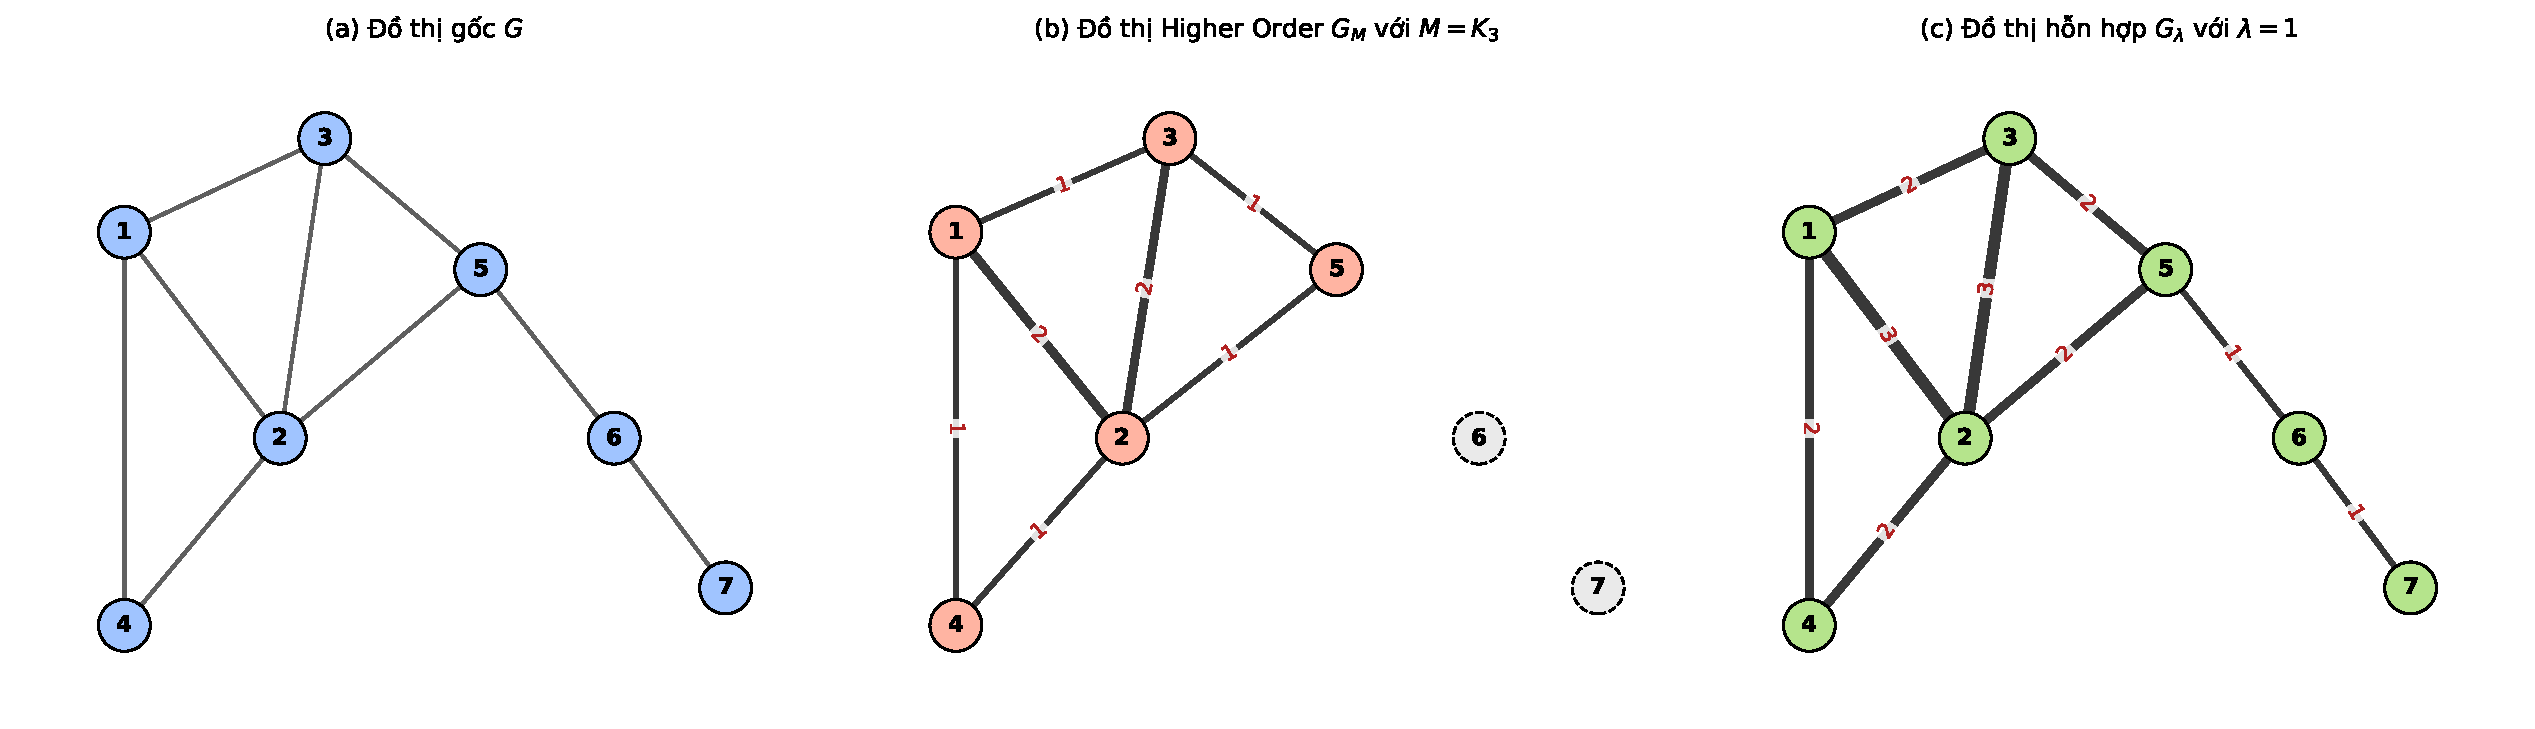
\includegraphics[width=\textwidth]{mixed_graph_construction.pdf}
    \caption[Xây dựng đồ thị hỗn hợp $G_\lambda$ từ $G$ và $G_M$.]{Xây dựng đồ thị hỗn hợp $G_\lambda$ từ $G$ và $G_M$ với $\lambda = 1$, $M = K_3$.}
    \label{fig:mixed-graph-construction}
\end{figure}

% ============================================================
\section{Tính chất phổ và hệ quả của thuật toán}
\label{sec:wlambda-properties}

% ............................................................
\subsection{$G_\lambda$ là đồ thị có trọng số hợp lệ}

\begin{proposition}
\label{prop:wlambda-valid}
Với mọi $\lambda \geq 0$, ma trận $W_\lambda$ đối xứng và không âm. Do đó $G_\lambda = (V, W_\lambda)$ là đồ thị có trọng số vô hướng hợp lệ.
\end{proposition}

\begin{proof}
$A$ và $W^{(M)}$ đều đối xứng (Mệnh đề~\ref{prop:gm-valid-weighted-graph} cho $W^{(M)}$, định nghĩa cho $A$) và có các phần tử không âm. Vì $\lambda \geq 0$, tổng có trọng số $A + \lambda W^{(M)}$ giữ tính đối xứng và không âm.
\end{proof}

Mệnh đề~\ref{prop:wlambda-valid} là điểm tựa cho toàn bộ phần còn lại của chương: vì $W_\lambda$ thuộc lớp ma trận trọng số đối xứng không âm, mọi định lý phổ phát biểu trong Chương~\ref{chap:co-so} cho lớp này áp dụng nguyên dạng cho $G_\lambda$.

% ............................................................
\subsection{Conductance trên $G_\lambda$}

Tương tự conductance trên $G$ và conductance motif trên $G_M$, ta định nghĩa conductance trên $G_\lambda$ bằng cách thay $A$ bởi $W_\lambda$ trong Định nghĩa~\ref{def:cut-volume} và Định nghĩa~\ref{def:conductance}.

\begin{definition}[Conductance trên $G_\lambda$]
\label{def:wlambda-conductance}
Với $S \subset V$, đặt
\[
    \mathrm{cut}_\lambda(S, \bar S) = \sum_{u \in S,\, v \in \bar S} (W_\lambda)_{uv}, \qquad
    \mathrm{vol}_\lambda(S) = \sum_{u \in S} (W_\lambda \mathbf{1})_u.
\]
Conductance trên $G_\lambda$ là
\[
    \phi_\lambda(S) = \frac{\mathrm{cut}_\lambda(S, \bar S)}{\min(\mathrm{vol}_\lambda(S), \mathrm{vol}_\lambda(\bar S))},
\]
và $\phi_\lambda^* = \min_{\emptyset \neq S \subsetneq V} \phi_\lambda(S)$.
\end{definition}

Một quan sát đơn giản nhưng then chốt: conductance trên $G_\lambda$ là tổ hợp tuyến tính của conductance trên $G$ và conductance motif trên $G_M$.

\begin{proposition}[Phân tích cộng tính của $\mathrm{cut}_\lambda$]
\label{prop:cut-decomposition}
Với mọi $S \subset V$,
\[
    \mathrm{cut}_\lambda(S, \bar S) = \mathrm{cut}(S, \bar S) + \lambda \, \mathrm{cut}_M(S, \bar S), \qquad
    \mathrm{vol}_\lambda(S) = \mathrm{vol}(S) + \lambda \, \mathrm{vol}_M(S).
\]
\end{proposition}

\begin{proof}
Hệ quả trực tiếp của $W_\lambda = A + \lambda W^{(M)}$ và tính tuyến tính của tổng theo các phần tử ma trận.
\end{proof}

% ............................................................
\subsection{Bất đẳng thức Cheeger trên $G_\lambda$}

\begin{theorem}[Cheeger trên $G_\lambda$]
\label{thm:wlambda-cheeger}
Đặt $D_\lambda = \mathrm{diag}(W_\lambda \mathbf{1})$ và $\mathcal{L}_\lambda = I - D_\lambda^{-1/2} W_\lambda D_\lambda^{-1/2}$ là Laplacian chuẩn hóa của $G_\lambda$. Khi đó $\mathcal{L}_\lambda$ đối xứng nửa xác định dương với phổ
\[
    0 = \lambda_1(\mathcal{L}_\lambda) \leq \lambda_2(\mathcal{L}_\lambda) \leq \cdots \leq \lambda_n(\mathcal{L}_\lambda) \leq 2,
\]
và conductance tối thiểu $\phi_\lambda^*$ thỏa
\[
    \frac{\lambda_2(\mathcal{L}_\lambda)}{2} \;\leq\; \phi_\lambda^* \;\leq\; \sqrt{2 \lambda_2(\mathcal{L}_\lambda)}.
\]
\end{theorem}

\begin{proof}
Theo Mệnh đề~\ref{prop:wlambda-valid}, $W_\lambda$ là ma trận đối xứng và không âm, do đó $G_\lambda = (V, W_\lambda)$ thuộc đúng lớp đồ thị mà Định lý~\ref{thm:cheeger} đã được phát biểu. Việc cần làm là chỉ ra mọi đại lượng và mọi lập luận trong chứng minh nguyên thuỷ đều chuyển nguyên dạng sang $G_\lambda$.

Các đại lượng phổ trên $G_\lambda$ được đặt theo đúng công thức như trên $G$, chỉ thay ma trận trọng số $A$ bởi $W_\lambda$. Ma trận bậc $D_\lambda = \mathrm{diag}(W_\lambda \mathbf{1})$ có phần tử đường chéo $(D_\lambda)_{uu} = d_u + \lambda d_u^{(M)}$ dương trên mọi đỉnh có $d_u \geq 1$ (Mệnh đề~\ref{prop:wlambda-fixes-gm}), nên $D_\lambda^{-1/2}$ định nghĩa tốt và Laplacian chuẩn hoá
\[
    \mathcal{L}_\lambda \;=\; I - D_\lambda^{-1/2} W_\lambda D_\lambda^{-1/2}
\]
là ma trận đối xứng nửa xác định dương với phổ nằm trong $[0, 2]$. Tương tự, conductance $\phi_\lambda$ trên $G_\lambda$ (Định nghĩa~\ref{def:wlambda-conductance}) mang cấu trúc đại số đồng nhất với conductance $\phi$ trên $G$, chỉ thay $\mathrm{cut}$ bởi $\mathrm{cut}_\lambda$ và $\mathrm{vol}$ bởi $\mathrm{vol}_\lambda$.

Chứng minh của Định lý~\ref{thm:cheeger} không dùng giả thiết nào ngoài tính đối xứng và tính không âm của ma trận trọng số, vốn đã được kế thừa cho $W_\lambda$. Cụ thể, cận dưới $\lambda_2 / 2 \leq \phi^*$ trên $G$ được rút ra bằng cách áp dụng bất đẳng thức biến phân Courant--Fischer (Định lý~\ref{thm:courant-fischer}) cho vector chỉ thị có trọng của một nhát cắt bất kỳ; cùng lập luận này áp dụng cho $\mathcal{L}_\lambda$ vì vector chỉ thị có trọng vẫn định nghĩa tốt với $D_\lambda$ dương trên các đỉnh liên thông, và biến phân Courant--Fischer thì đúng cho mọi ma trận đối xứng. Cận trên $\phi^* \leq \sqrt{2 \lambda_2}$ trên $G$ rút ra bằng phép cắt sweep trên vector riêng thứ hai; trên $G_\lambda$, ánh xạ $D_\lambda^{-1/2} v_2(\mathcal{L}_\lambda)$ vẫn là một hàm thực trên $V$ nên sweep được định nghĩa tốt và sinh một họ hữu hạn nhát cắt $S_t$ để so sánh.

Do đó hai cận của Định lý~\ref{thm:cheeger} chuyển nguyên dạng sang $G_\lambda$:
\[
    \frac{\lambda_2(\mathcal{L}_\lambda)}{2} \;\leq\; \phi_\lambda^* \;\leq\; \sqrt{2 \lambda_2(\mathcal{L}_\lambda)}. \qedhere
\]
\end{proof}

% ............................................................
\subsection{Tính đúng đắn của phân cụm phổ trên $G_\lambda$}

\begin{theorem}[Bảo đảm xấp xỉ conductance]
\label{thm:wlambda-spectral-correctness}
Áp dụng Thuật toán~\ref{alg:spectral-clustering} với đầu vào $W = W_\lambda$ và $K = 2$, gọi $S^{\mathrm{sweep}}_\lambda$ là nhát cắt thu được. Khi đó
\[
    \phi_\lambda^* \;\leq\; \phi_\lambda(S^{\mathrm{sweep}}_\lambda) \;\leq\; \sqrt{2 \lambda_2(\mathcal{L}_\lambda)} \;\leq\; 2 \sqrt{\phi_\lambda^*}.
\]
Tổng quát hóa cho $K$ cụm: phân hoạch $\{C_k\}$ thu được từ Thuật toán~\ref{alg:spectral-clustering} thỏa
\[
    \max_k \phi_\lambda(C_k) \;\leq\; O(K^2) \sqrt{\lambda_K(\mathcal{L}_\lambda)},
\]
theo bất đẳng thức Cheeger bậc cao.
\end{theorem}

\begin{proof}
\emph{Trường hợp $K = 2$.} Thuật toán~\ref{alg:spectral-clustering} chạy trên đầu vào $W = W_\lambda$ tính phổ của $\mathcal{L}_\lambda$, lấy vector riêng $v_2(\mathcal{L}_\lambda)$ ứng với $\lambda_2(\mathcal{L}_\lambda)$, và xét các nhát cắt sweep trên $D_\lambda^{-1/2} v_2(\mathcal{L}_\lambda)$. Định lý~\ref{thm:sweep-bound} áp dụng cho $G_\lambda$ (hợp lệ nhờ Mệnh đề~\ref{prop:wlambda-valid}) cho cận
\[
    \phi_\lambda\bigl(S^{\mathrm{sweep}}_\lambda\bigr) \;\leq\; \sqrt{2 \lambda_2(\mathcal{L}_\lambda)}.
\]
Theo định nghĩa của conductance tối thiểu, $\phi_\lambda^* \leq \phi_\lambda(S^{\mathrm{sweep}}_\lambda)$. Mặt khác, cận dưới Cheeger $\lambda_2(\mathcal{L}_\lambda) / 2 \leq \phi_\lambda^*$ (Định lý~\ref{thm:wlambda-cheeger}) viết lại thành $\lambda_2(\mathcal{L}_\lambda) \leq 2 \phi_\lambda^*$, từ đó
\[
    \sqrt{2 \lambda_2(\mathcal{L}_\lambda)} \;\leq\; \sqrt{4 \phi_\lambda^*} \;=\; 2 \sqrt{\phi_\lambda^*}.
\]
Ghép ba bất đẳng thức:
\[
    \phi_\lambda^* \;\leq\; \phi_\lambda(S^{\mathrm{sweep}}_\lambda) \;\leq\; \sqrt{2 \lambda_2(\mathcal{L}_\lambda)} \;\leq\; 2 \sqrt{\phi_\lambda^*}.
\]

\emph{Trường hợp $K$ cụm.} Bất đẳng thức Cheeger bậc cao của Lee, Oveis Gharan và Trevisan (trình bày trong Mục~\ref{subsec:correctness} cho đồ thị có trọng số tổng quát) cho phép, với phân hoạch $\{C_k\}$ thu được từ phân cụm phổ trên $K$ vector riêng đầu của $\mathcal{L}_\lambda$:
\[
    \max_k \phi_\lambda(C_k) \;\leq\; O(K^2) \sqrt{\lambda_K(\mathcal{L}_\lambda)}.
\]
Việc áp dụng bất đẳng thức này cho $\mathcal{L}_\lambda$ hợp lệ vì $\mathcal{L}_\lambda$ là Laplacian chuẩn hoá của đồ thị có trọng số đối xứng không âm (Mệnh đề~\ref{prop:wlambda-valid}), và lập luận chứng minh trong tài liệu gốc chỉ dùng các tính chất phổ của Laplacian không phụ thuộc dạng riêng của ma trận trọng số.
\end{proof}

Định lý~\ref{thm:wlambda-spectral-correctness} nói rằng phân cụm phổ trên $G_\lambda$ tìm phân hoạch có conductance gần tối ưu theo metric $\phi_\lambda$ tương ứng. Đây là sự kế thừa trực tiếp của các bảo đảm trên đồ thị có trọng số tổng quát: việc đưa thêm thành phần $\lambda W^{(M)}$ vào ma trận đầu vào không làm mất đi bất kỳ bảo đảm nào đã có cho phân cụm phổ cổ điển.

% ............................................................
\subsection{Cải thiện so với đồ thị Higher Order}
\label{subsec:improvement-vs-gm}

So với phân cụm phổ trên $G_M$ thuần, phân cụm phổ trên $G_\lambda$ với $\lambda > 0$ có hai cải thiện trực tiếp, hệ quả của việc cộng thêm $A$ vào ma trận đầu vào.

\begin{proposition}[Khắc phục hạn chế của $G_M$]
\label{prop:wlambda-fixes-gm}
Với mọi $\lambda > 0$:
\begin{enumerate}[topsep=4pt, itemsep=4pt, parsep=0pt]
    \item Bảo toàn tính liên thông. Nếu $G$ liên thông thì $G_\lambda$ cũng liên thông.
    \item Bảo toàn thông tin cạnh gốc. Mọi cạnh $(u, v) \in E$ đều có $(W_\lambda)_{uv} \geq A_{uv} \geq 1$, nên không bị xóa trong $G_\lambda$ kể cả khi không thuộc instance nào của $M$.
\end{enumerate}
\end{proposition}

\begin{proof}
\emph{Phần (1).} Vì $W^{(M)} \geq 0$ và $\lambda \geq 0$, ta có $(W_\lambda)_{uv} = A_{uv} + \lambda W^{(M)}_{uv} \geq A_{uv}$ với mọi $u, v$. Do đó mọi cạnh của $G$ đều là cạnh của $G_\lambda$ (với trọng số dương ít nhất bằng trong $G$). Nếu $G$ liên thông thì giữa hai đỉnh bất kỳ tồn tại đường đi trong $G$, và đường đi đó cũng là đường đi trong $G_\lambda$, nên $G_\lambda$ liên thông. Trái lại, trong $G_M$ thuần một đỉnh không thuộc tam giác nào sẽ có $d_u^{(M)} = 0$ và trở thành cô lập, làm $G_M$ có thể mất liên thông kể cả khi $G$ liên thông.

\emph{Phần (2).} Trực tiếp từ $W_\lambda = A + \lambda W^{(M)}$:
\[
    (W_\lambda)_{uv} = A_{uv} + \lambda W^{(M)}_{uv} \;\geq\; A_{uv},
\]
vì $\lambda W^{(M)}_{uv} \geq 0$. Khi $(u, v) \in E$, $A_{uv} \geq 1$, nên $(W_\lambda)_{uv} \geq 1$. Cạnh $(u, v)$ do đó được bảo toàn trong $G_\lambda$ với trọng số ít nhất bằng trọng số gốc, không bị xoá kể cả khi $(u, v)$ không thuộc instance nào của $M$ (trường hợp $W^{(M)}_{uv} = 0$).
\end{proof}

Hai khẳng định trong Mệnh đề~\ref{prop:wlambda-fixes-gm} đối ứng với hai hạn chế của $G_M$ phát biểu trong Nhận xét~\ref{rem:gm-limit}, và có thể quan sát trực tiếp trên Hình~\ref{fig:mixed-graph-construction}: các đỉnh $6, 7$ vốn cô lập trong $G_M$ trở lại liên thông trong $G_\lambda$, và các cạnh $5{-}6$, $6{-}7$ vốn bị xóa trong $G_M$ được bảo toàn trong $G_\lambda$ với trọng số $1$.

% ============================================================
\section{Hệ quả về các chỉ số $\overline{\mathrm{CC}}_w$ và $Q$}
\label{sec:wlambda-cc-q}

\emph{(Phần này dành cho các định lý chứng minh hệ quả của việc dùng $G_\lambda$ thay cho $G_M$ thuần đối với các chỉ số $\overline{\mathrm{CC}}_w$ và $Q$. Sẽ được hoàn thiện ở phiên bản sau.)}

\cleardoublepage

% ============================================================
%  CHƯƠNG 3: THỰC NGHIỆM
% ============================================================

\chapter{Thực nghiệm và đánh giá}
\label{chap:thuc-nghiem}

Chương này trình bày kết quả thực nghiệm Thuật toán~\ref{alg:spectral-clustering} với đầu vào $W = W_\lambda = A + \lambda W^{(M)}$ ($M = K_3$) trên hai loại dữ liệu. Loại thứ nhất gồm bốn mô hình sinh ngẫu nhiên có cấu trúc cộng đồng (SBM, Planted Partition, GRPG, LFR). Loại thứ hai gồm mười đồ thị mạng xã hội thật. Định nghĩa hình thức của các mô hình sinh ngẫu nhiên xem Phụ lục~\ref{appx:random-models}.

% ============================================================
\section{Thiết lập thí nghiệm}
\label{sec:setup}

\textbf{Quét tham số.} $\lambda \in \{0,\ 0.5,\ 1,\ 2,\ 5,\ 10\}$ kèm trường hợp $W_M$ thuần (tương ứng $\lambda \to \infty$). Trường hợp $\lambda = 0$ trùng với phân cụm phổ cổ điển trên ma trận kề $A$ và được dùng làm chuẩn so sánh.

\textbf{Số cụm $K$.} Với đồ thị có phân hoạch chuẩn, đặt $K = K_{\mathrm{gt}}$ là số cộng đồng thật. Với đồ thị mạng xã hội không có phân hoạch chuẩn, quét $K \in \{50, 100, 200, 300, 400, 500\}$ cho mỗi đồ thị.

\textbf{Chỉ số đánh giá.} Mọi chỉ số được tính trên đồ thị gốc $A$, không phải trên $W_\lambda$:
\begin{itemize}
    \item Modularity $Q$ là chỉ số chất lượng chính.
    \item NMI và Jaccard so với phân hoạch chuẩn (khi có).
    \item $\overline{\mathrm{CC}}$, $\overline{\mathrm{CC}}_w$: hệ số phân cụm tổng hợp.
    \item Số cạnh bị cắt và số motif (tam giác) bị cắt qua biên cụm.
\end{itemize}

\textbf{Mục tiêu.} Với mỗi bộ test, ghi lại $Q(\lambda)$ cho từng giá trị $\lambda$. Đặt
\[
    \Delta Q = \max_{\lambda > 0} Q(\lambda) - Q(0)
\]
là mức tăng tốt nhất do ma trận hỗn hợp đem lại so với phân cụm phổ cổ điển. $\Delta Q > 0$ chứng tỏ $W_\lambda$ với $\lambda > 0$ phù hợp hơn $A$; $\lambda^*$ đạt cực đại là giá trị tối ưu cho bộ test.

% ============================================================
\section{Đồ thị có cấu trúc cộng đồng}
\label{sec:results-synthetic}

Bảng~\ref{tab:synthetic-summary} tổng hợp kết quả tốt nhất trên bốn mô hình. Với mỗi mô hình, năm bộ test có $\Delta Q$ lớn nhất (lọc $Q(0) \geq 0{,}1$ để tránh phân hoạch tầm thường) được chọn.

\begin{table}[H]
\centering
\caption{Kết quả tốt nhất trên bốn mô hình có cấu trúc cộng đồng}
\label{tab:synthetic-summary}
\begin{tabular}{|l|l|c|c|c|c|}
\hline
\textbf{Mô hình} & \textbf{Bộ test tốt nhất} & $Q(0)$ & $\lambda^*$ & $Q(\lambda^*)$ & $\Delta Q$ \\ \hline
LFR     & LFR-100-$\mu{=}0{,}35$       & 0{,}1124 & 5{,}0    & 0{,}4785 & $+0{,}3661$ \\ \hline
GRPG    & GRPG-2000-$p_{\mathrm{out}}{=}0{,}006$ & 0{,}1165 & 1{,}0 & 0{,}2005 & $+0{,}0840$ \\ \hline
Planted & Planted-$k{=}5$-$p_{\mathrm{out}}{=}0{,}025$ & 0{,}1203 & 0{,}5 & 0{,}2185 & $+0{,}0982$ \\ \hline
SBM     & SBM-1500-$p_{\mathrm{out}}{=}0{,}008$ & 0{,}1673 & 0{,}5 & 0{,}1975 & $+0{,}0302$ \\ \hline
\end{tabular}
\end{table}

% ............................................................
\subsection{LFR Benchmark}
\label{subsec:results-lfr}

Bộ dữ liệu Lancichinetti--Fortunato--Radicchi (LFR) được công nhận rộng rãi như benchmark chuẩn cho bài toán phát hiện cộng đồng nhờ phân bố bậc và phân bố kích thước cụm cùng tuân theo luỹ thừa, gần với cấu trúc của nhiều mạng thật. Tham số then chốt là mixing parameter $\mu \in (0, 1)$: mỗi đỉnh dành tỉ lệ $1 - \mu$ số cạnh cho cộng đồng của mình và tỉ lệ $\mu$ số cạnh cho phần còn lại của đồ thị. Giá trị $\mu$ càng lớn, ranh giới cộng đồng càng mờ và bài toán càng khó. Khoá luận quét $n \in \{100, 500, 2000\}$ và $\mu \in \{0{,}2,\ 0{,}35,\ 0{,}4,\ 0{,}5\}$, các tham số còn lại giữ mặc định của thuật toán sinh.

\subsubsection*{Modularity và NMI}

Bảng~\ref{tab:lfr-top5} trình bày năm bộ test LFR có $\Delta Q$ lớn nhất. Hình~\ref{fig:lfr-modularity} và Hình~\ref{fig:lfr-nmi} lần lượt cho biểu đồ modularity và NMI theo $\lambda$.

\begin{table}[H]
\centering
\caption{Năm bộ test LFR có cải thiện modularity lớn nhất}
\label{tab:lfr-top5}
\begin{tabular}{|l|c|c|c|c|c|c|}
\hline
\textbf{Bộ test} & $Q(0)$ & $\lambda{=}0{,}5$ & $\lambda{=}1$ & $\lambda{=}2$ & $\lambda{=}5$ & $\lambda^*$ \\ \hline
LFR-100-$\mu0{,}35$  & 0{,}1124 & 0{,}0042 & 0{,}0838 & 0{,}2942 & \textbf{0{,}4785} & $5{,}0$ \\ \hline
LFR-100-$\mu0{,}2$   & 0{,}4747 & 0{,}4858 & 0{,}4761 & \textbf{0{,}6280} & 0{,}6255 & $2{,}0$ \\ \hline
LFR-500-$\mu0{,}4$   & 0{,}1670 & \textbf{0{,}2979} & 0{,}2951 & 0{,}2778 & 0{,}2708 & $0{,}5$ \\ \hline
LFR-2000-$\mu0{,}5$  & 0{,}1112 & 0{,}2348 & \textbf{0{,}2409} & 0{,}2382 & 0{,}2275 & $1{,}0$ \\ \hline
LFR-500-$\mu0{,}35$  & 0{,}2181 & \textbf{0{,}3380} & 0{,}2992 & 0{,}3270 & 0{,}3199 & $0{,}5$ \\ \hline
\end{tabular}
\end{table}

\begin{figure}[H]
    \centering
    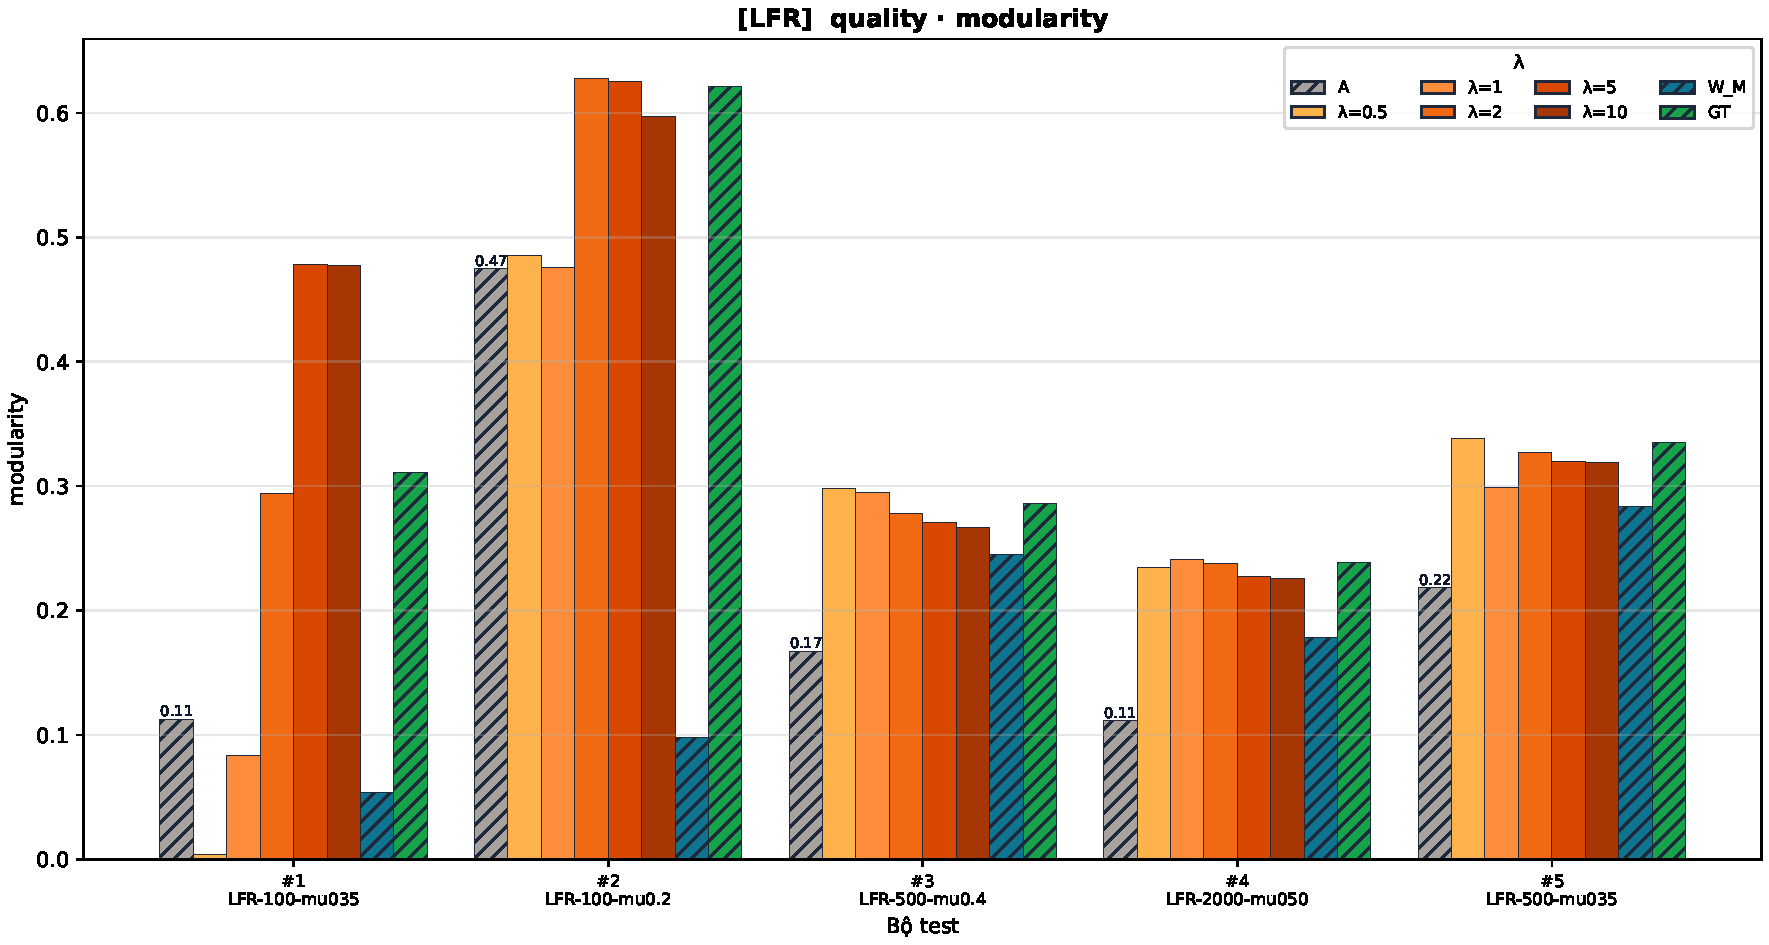
\includegraphics[width=\textwidth]{../main_result/LFR/charts/quality_modularity.pdf}
    \caption[Modularity $Q$ trên năm bộ LFR theo $\lambda$.]{Modularity $Q$ trên năm bộ LFR có $\Delta Q$ lớn nhất theo $\lambda$.}
    \label{fig:lfr-modularity}
\end{figure}

\begin{figure}[H]
    \centering
    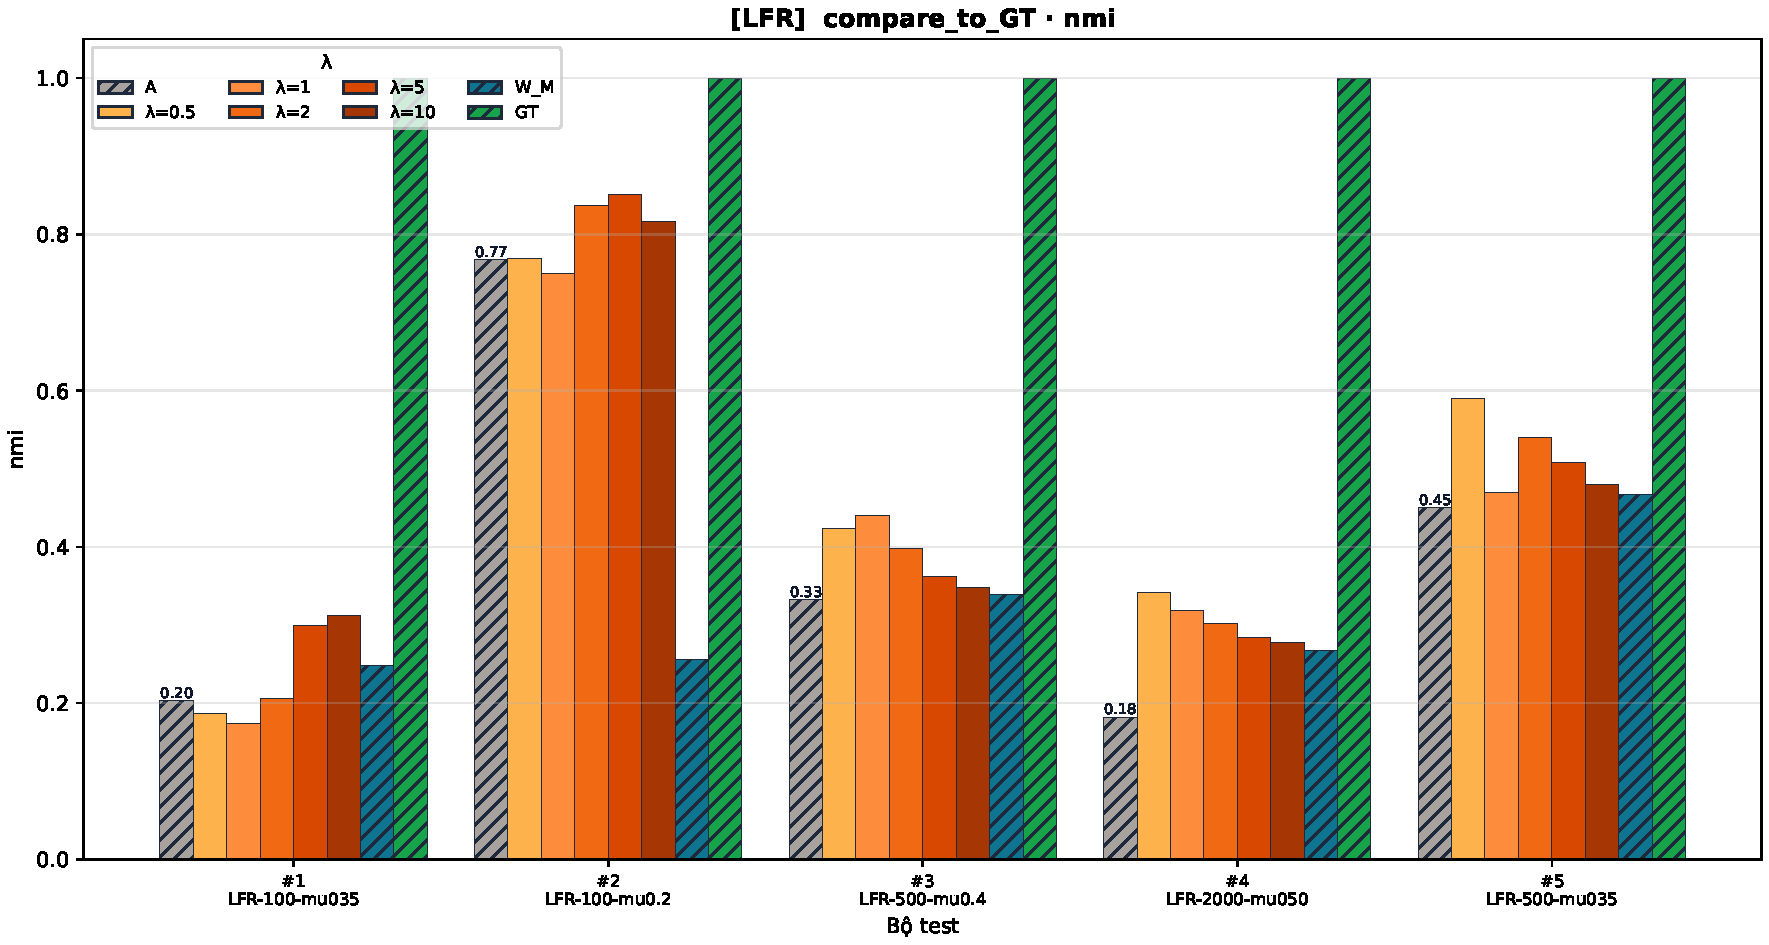
\includegraphics[width=\textwidth]{../main_result/LFR/charts/compare_to_GT_nmi.pdf}
    \caption{NMI so với phân hoạch chuẩn trên năm bộ LFR theo $\lambda$.}
    \label{fig:lfr-nmi}
\end{figure}

\textbf{Quan sát.} $Q$ tăng trên toàn dải $\mu$, biên độ lớn nhất tập trung ở vùng cộng đồng tách yếu. Bộ LFR-100-$\mu0{,}35$ minh hoạ rõ nhất khi $Q$ chuyển từ $0{,}1124$ tại $\lambda = 0$ lên $0{,}4785$ tại $\lambda = 5$, và NMI đồng pha tăng từ $0{,}2026$ lên $0{,}3124$. Giá trị $\lambda^*$ tối ưu phân tán trong khoảng $0{,}5$ đến $5$ tuỳ bộ test.

\textbf{Nhận xét.} Mức cải thiện chỉ rõ rệt khi modularity ban đầu thấp. Khi $\mu$ nhỏ, các cạnh nội cụm đã đủ rõ để phân cụm phổ trên $A$ hoạt động tốt, đóng góp của motif bị bão hoà. Sự đồng pha của $Q$ và NMI là yếu tố then chốt: phân hoạch thu được không chỉ tối ưu theo chỉ số nội tại mà còn gần phân hoạch chuẩn hơn, loại trừ khả năng modularity tăng do thuật toán bị đẩy về một phân hoạch tốt giả tạo. Phân tán của $\lambda^*$ cho thấy cần chiến lược chọn $\lambda$ phụ thuộc đồ thị, không tồn tại quy tắc cố định toàn cục.

\subsubsection*{Hệ số phân cụm}

\begin{figure}[H]
    \centering
    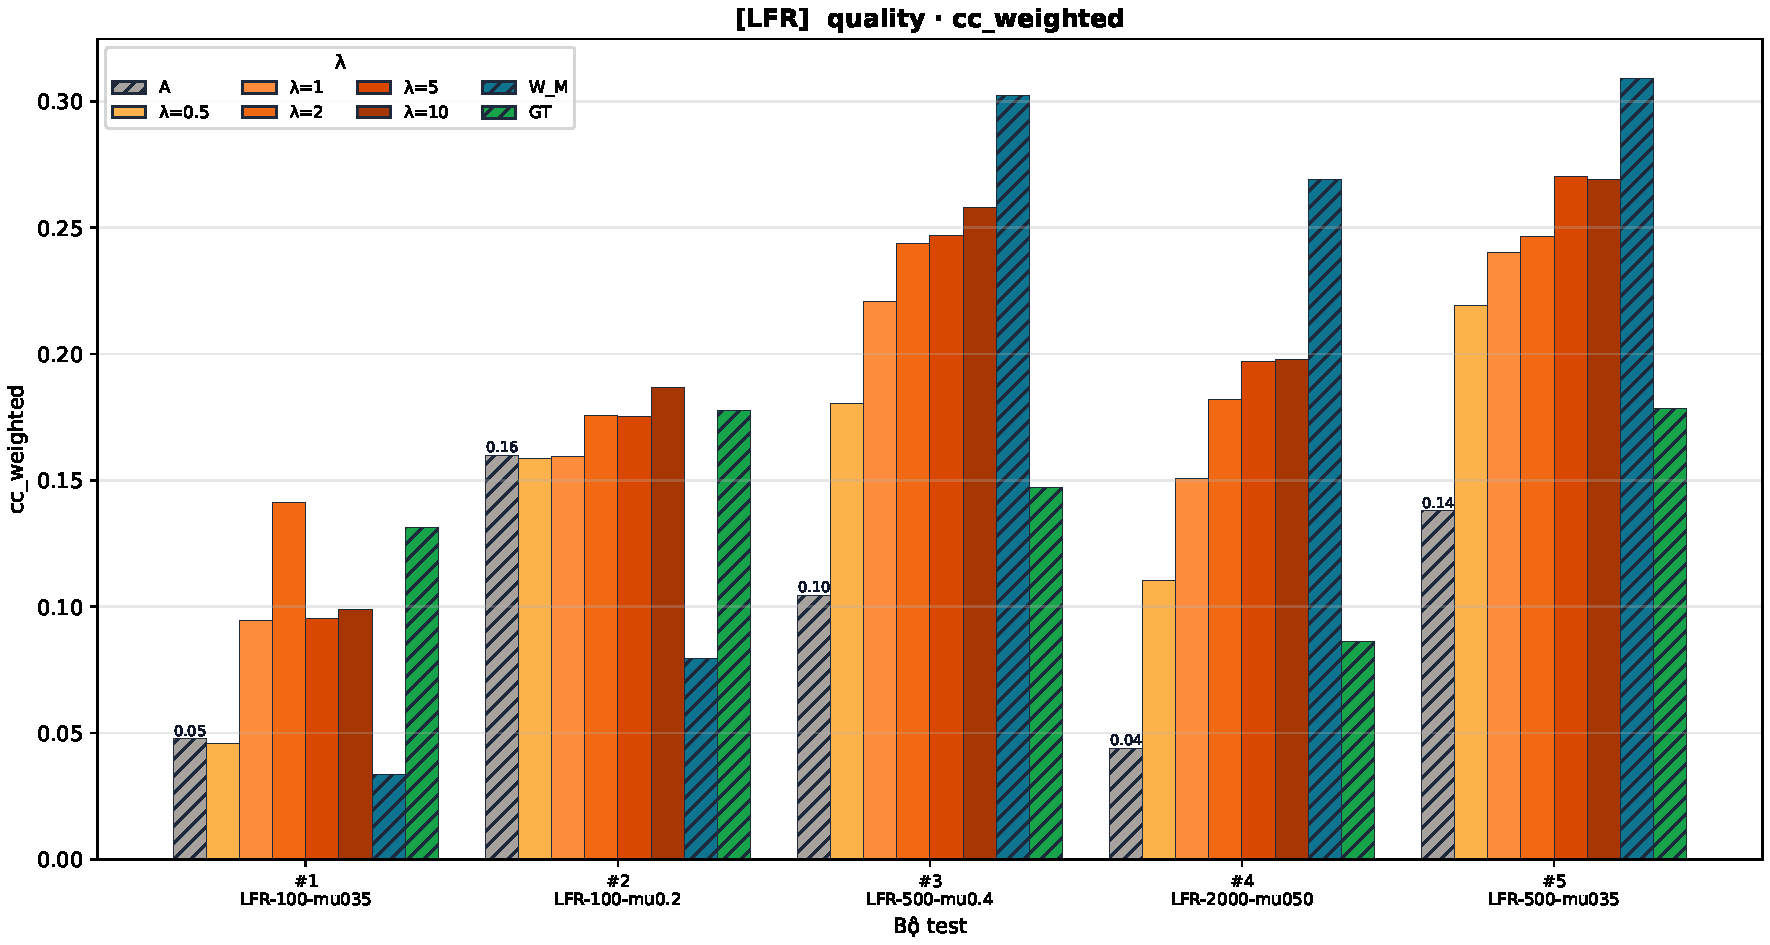
\includegraphics[width=\textwidth]{../main_result/LFR/charts/quality_cc_weighted.pdf}
    \caption{$\overline{\mathrm{CC}}_w$ trên năm bộ LFR theo $\lambda$.}
    \label{fig:lfr-cc-weighted}
\end{figure}

\begin{figure}[H]
    \centering
    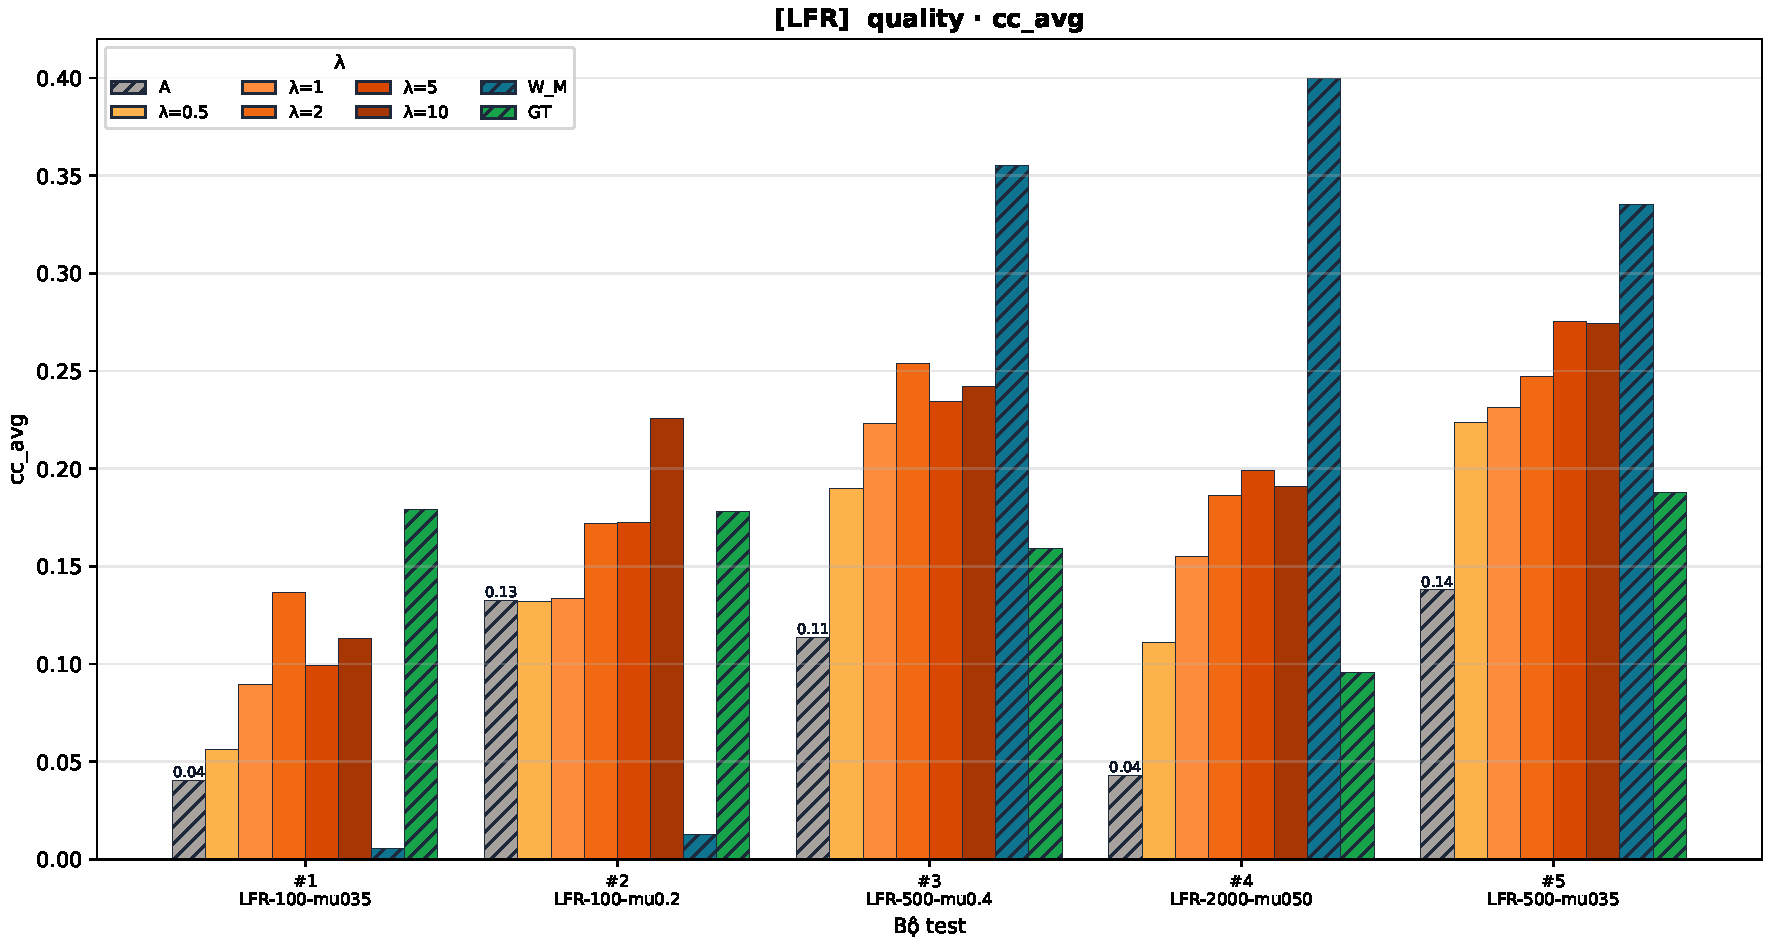
\includegraphics[width=\textwidth]{../main_result/LFR/charts/quality_cc_avg.pdf}
    \caption{$\overline{\mathrm{CC}}$ trên năm bộ LFR theo $\lambda$.}
    \label{fig:lfr-cc-avg}
\end{figure}

\textbf{Quan sát.} Hệ số phân cụm toàn cục của đồ thị gốc $cc_{\mathrm{global}} = 0{,}0513$ đóng vai trò baseline. Trên bộ LFR-100-$\mu0{,}35$, $\overline{\mathrm{CC}}_w$ chuyển từ $0{,}0477$ tại $\lambda = 0$ (sát baseline) lên cực đại $0{,}1412$ tại $\lambda = 2$, gấp khoảng ba lần. $\overline{\mathrm{CC}}$ biến thiên gần đồng pha với $\overline{\mathrm{CC}}_w$, đạt $0{,}1364$ tại $\lambda = 2$. Modularity đạt đỉnh trễ hơn, ở $\lambda = 5$.

\textbf{Nhận xét.} Việc $\overline{\mathrm{CC}}_w$ tại đỉnh vượt baseline $cc_{\mathrm{global}}$ rõ rệt cho thấy thuật toán thực sự cô lập được các vùng đậm đặc tam giác vào trong cụm, không chỉ phản ánh phân bố tam giác sẵn có của đồ thị. Lệch pha giữa đỉnh $\overline{\mathrm{CC}}_w$ và đỉnh modularity phản ánh hai khía cạnh khác nhau: $\overline{\mathrm{CC}}_w$ chỉ đo mật độ tam giác nội cụm nên tăng theo trọng số motif một cách trực tiếp, còn modularity cân bằng giữa mật độ cạnh nội cụm và kỳ vọng ngẫu nhiên, do đó phản ứng chậm hơn và chỉ đạt đỉnh khi đóng góp của motif bù trừ được tác động làm loãng cạnh gốc. Khoảng cách giữa $\overline{\mathrm{CC}}$ và $\overline{\mathrm{CC}}_w$ không đáng kể, dấu hiệu cho thấy phân bố kích thước cụm luỹ thừa của LFR không sinh ra nhiều cụm rất nhỏ đủ để làm thiên lệch trung bình không trọng số; do đó hai đại lượng cho cùng kết luận trên dataset này.

% ............................................................
\subsection{Stochastic Block Model}
\label{subsec:results-sbm}

Stochastic Block Model là mô hình tổng quát nhất trong lớp đồ thị có cấu trúc cộng đồng đối xứng. Mỗi đỉnh được gán vào một trong $K$ khối, và xác suất xuất hiện cạnh giữa hai đỉnh chỉ phụ thuộc vào cặp khối mà chúng thuộc về. Tham số then chốt là cặp $(p_{\mathrm{in}}, p_{\mathrm{out}})$ với $p_{\mathrm{in}}$ là xác suất cạnh nội cụm và $p_{\mathrm{out}}$ là xác suất cạnh liên cụm; tỉ số $p_{\mathrm{out}}/p_{\mathrm{in}}$ càng cao thì bài toán càng khó. Khoá luận quét $n \in \{300, 600, 1500, 3000\}$ với $K = 3$ và $p_{\mathrm{out}}$ thuộc $\{0{,}005,\ 0{,}008,\ 0{,}02\}$, đi kèm $p_{\mathrm{in}}$ điều chỉnh theo $n$ để giữ bậc trung bình hợp lý.

\subsubsection*{Modularity và NMI}

\begin{table}[H]
\centering
\caption{Năm bộ test SBM có cải thiện modularity lớn nhất}
\label{tab:sbm-top5}
\begin{tabular}{|l|c|c|c|c|c|c|}
\hline
\textbf{Bộ test} & $Q(0)$ & $\lambda{=}0{,}5$ & $\lambda{=}1$ & $\lambda{=}2$ & $\lambda{=}5$ & $\lambda^*$ \\ \hline
SBM-1500-$p_{\mathrm{out}}0{,}008$  & 0{,}1673 & \textbf{0{,}1975} & 0{,}1925 & 0{,}1638 & 0{,}1330 & $0{,}5$ \\ \hline
SBM-3000-$p_{\mathrm{out}}0{,}005$  & 0{,}1757 & \textbf{0{,}1951} & 0{,}1932 & 0{,}1768 & 0{,}1448 & $0{,}5$ \\ \hline
SBM-300-$p_{\mathrm{out}}0{,}02$    & 0{,}3033 & \textbf{0{,}3064} & 0{,}3016 & 0{,}2929 & 0{,}2618 & $0{,}5$ \\ \hline
SBM-600-$p_{\mathrm{out}}0{,}02$    & 0{,}2168 & \textbf{0{,}2177} & 0{,}2109 & 0{,}1907 & 0{,}1672 & $0{,}5$ \\ \hline
SBM-300-$p_{\mathrm{out}}0{,}005$   & 0{,}5497 & \textbf{0{,}5505} & 0{,}5505 & 0{,}5505 & 0{,}5505 & $0{,}5$ \\ \hline
\end{tabular}
\end{table}

\begin{figure}[H]
    \centering
    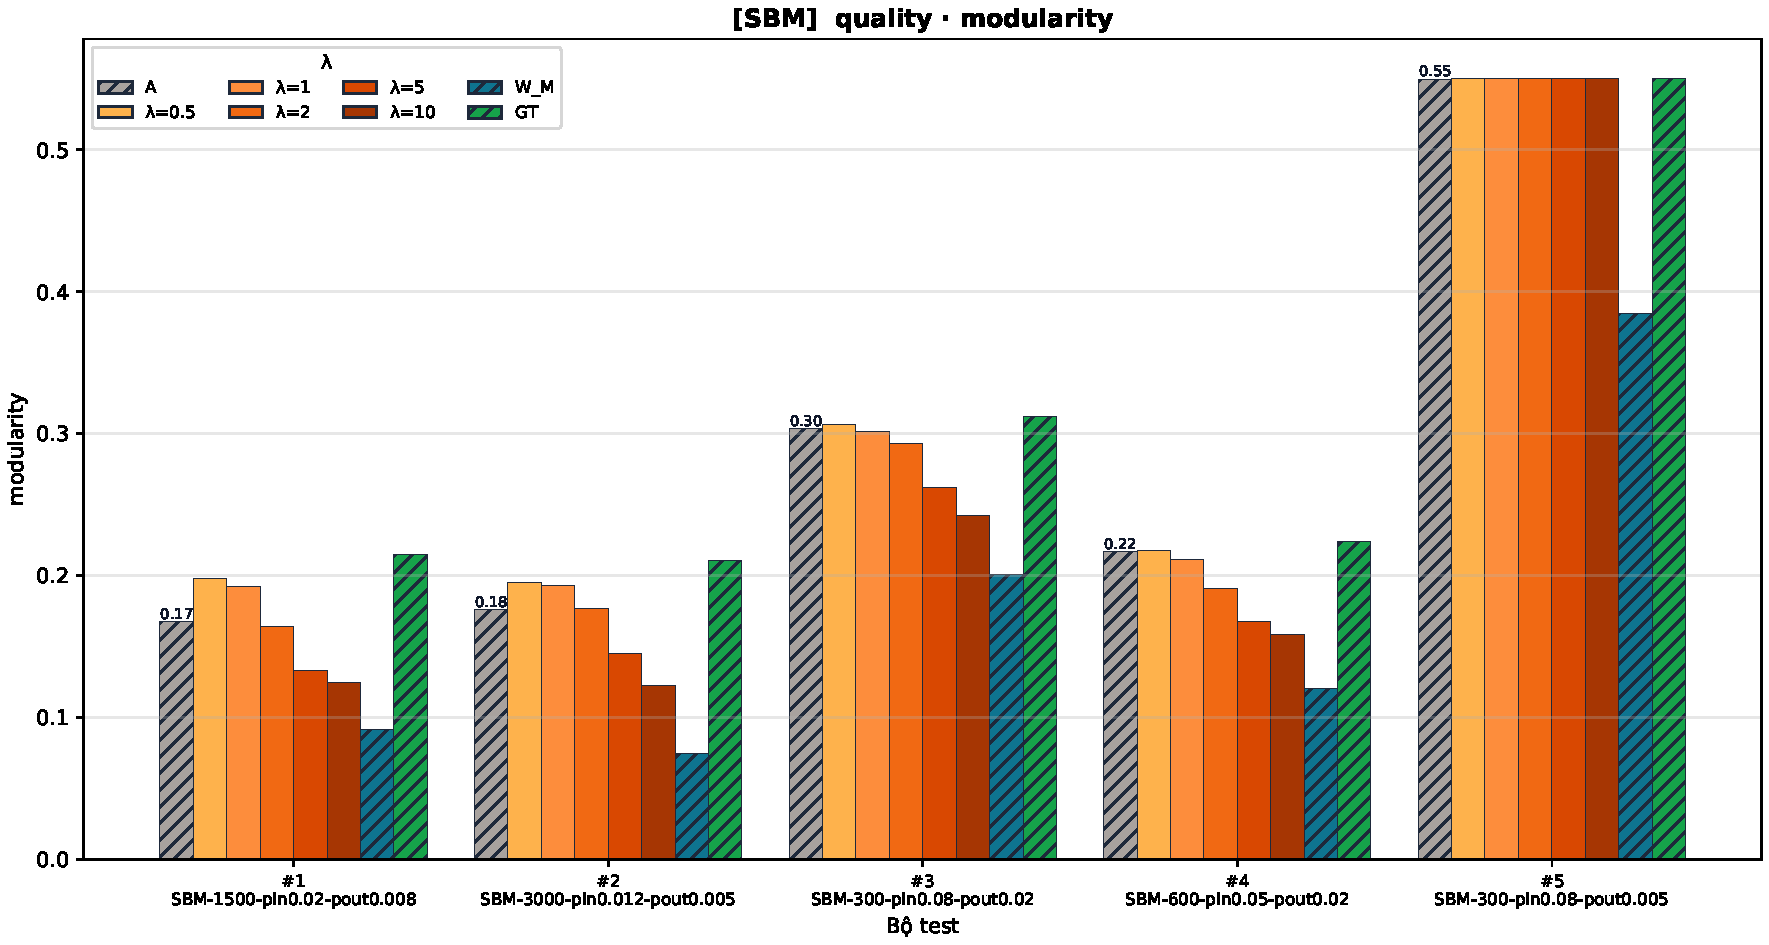
\includegraphics[width=\textwidth]{../main_result/SBM/charts/quality_modularity.pdf}
    \caption[Modularity $Q$ trên năm bộ SBM theo $\lambda$.]{Modularity $Q$ trên năm bộ SBM có $\Delta Q$ lớn nhất theo $\lambda$.}
    \label{fig:sbm-modularity}
\end{figure}

\begin{figure}[H]
    \centering
    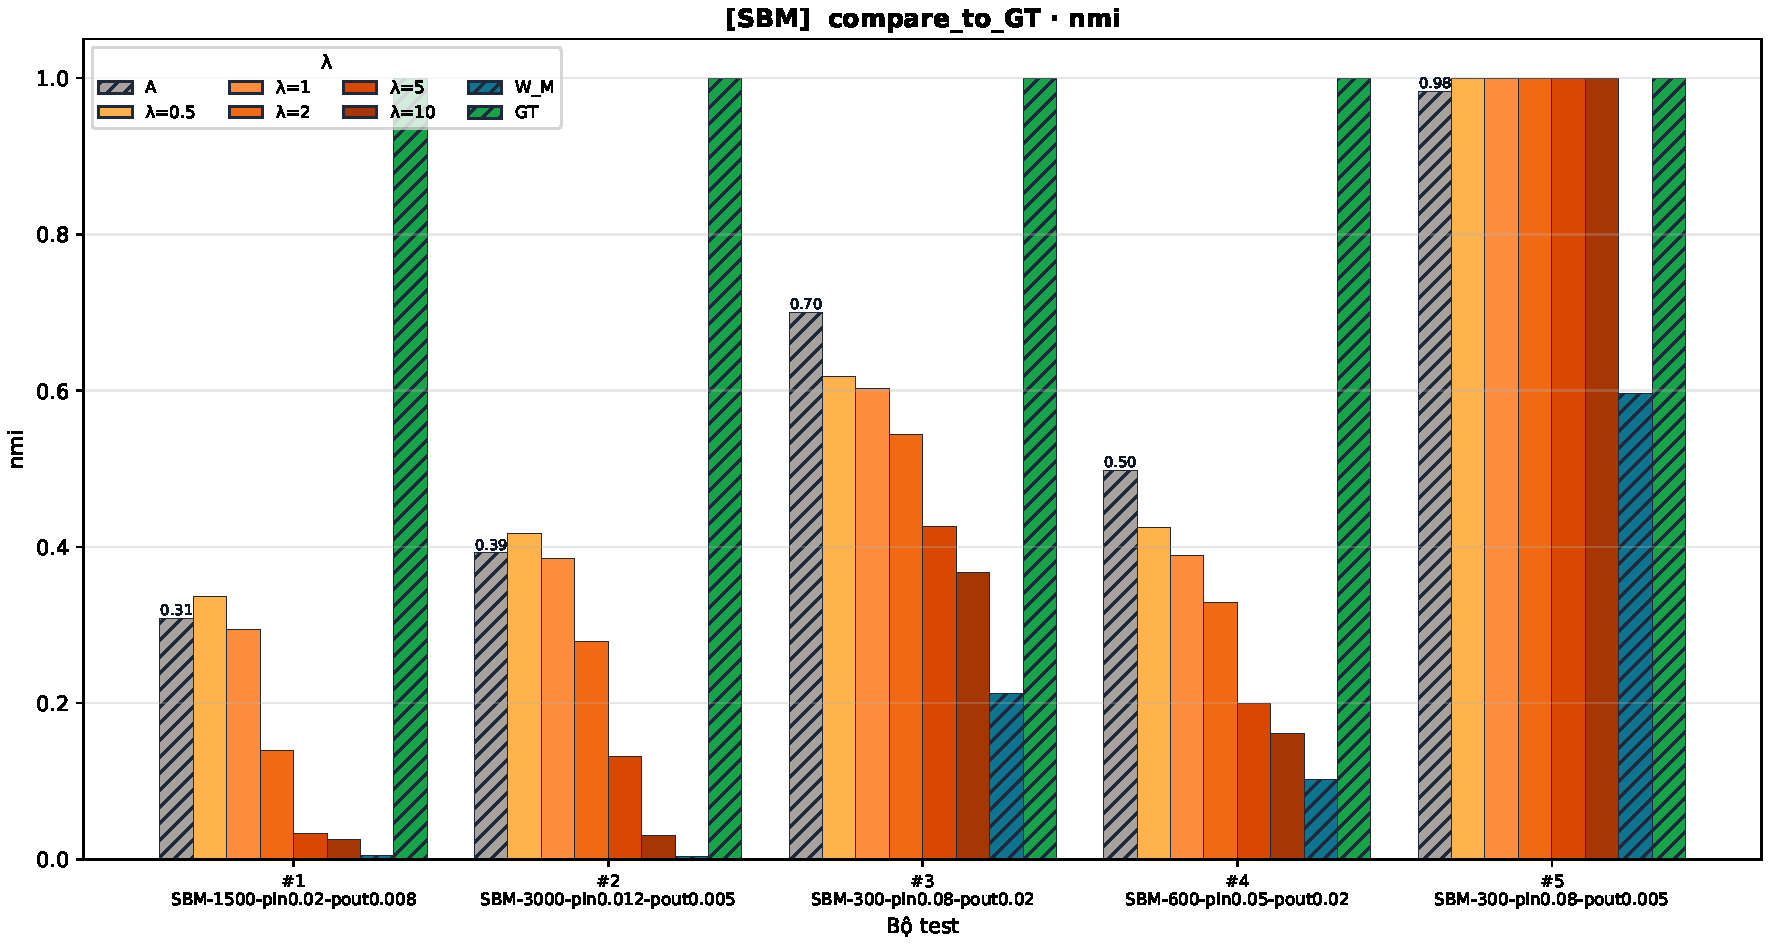
\includegraphics[width=\textwidth]{../main_result/SBM/charts/compare_to_GT_nmi.pdf}
    \caption{NMI so với phân hoạch chuẩn trên năm bộ SBM theo $\lambda$.}
    \label{fig:sbm-nmi}
\end{figure}

\textbf{Quan sát.} Toàn bộ năm bộ test cho $\lambda^* = 0{,}5$ và biên độ cải thiện $\Delta Q$ duy trì trong vùng hẹp từ $+0{,}0007$ đến $+0{,}0302$. Khi $\lambda$ vượt $0{,}5$, modularity giảm đều và NMI sụt rất nhanh: trên bộ SBM-1500-$p_{\mathrm{out}}0{,}008$, NMI từ $0{,}3360$ tại $\lambda = 0{,}5$ tụt xuống còn $0{,}0044$ tại $W_M$.

\textbf{Nhận xét.} Hành vi trên SBM khác hẳn LFR và phản ánh trực tiếp đặc tính sinh dữ liệu. Cơ chế sinh cạnh độc lập theo cặp của SBM khiến mọi tam giác xuất hiện đều là hệ quả thống kê của mật độ cạnh chứ không phải tín hiệu cấu trúc riêng. Vì thế tăng trọng số motif không cung cấp thông tin mới và còn phản tác dụng khi $\lambda$ lớn, do thành phần motif làm pha loãng tín hiệu cạnh vốn đã đủ để khôi phục cộng đồng. Sự sụp đổ nhanh của NMI là chỉ dấu rõ nhất rằng motif và phân hoạch chuẩn của SBM không chia sẻ chung một nguồn tín hiệu; bất cứ tối ưu nào theo $W_M$ thuần đều dẫn xa khỏi cộng đồng thật.

\subsubsection*{Hệ số phân cụm}

\begin{figure}[H]
    \centering
    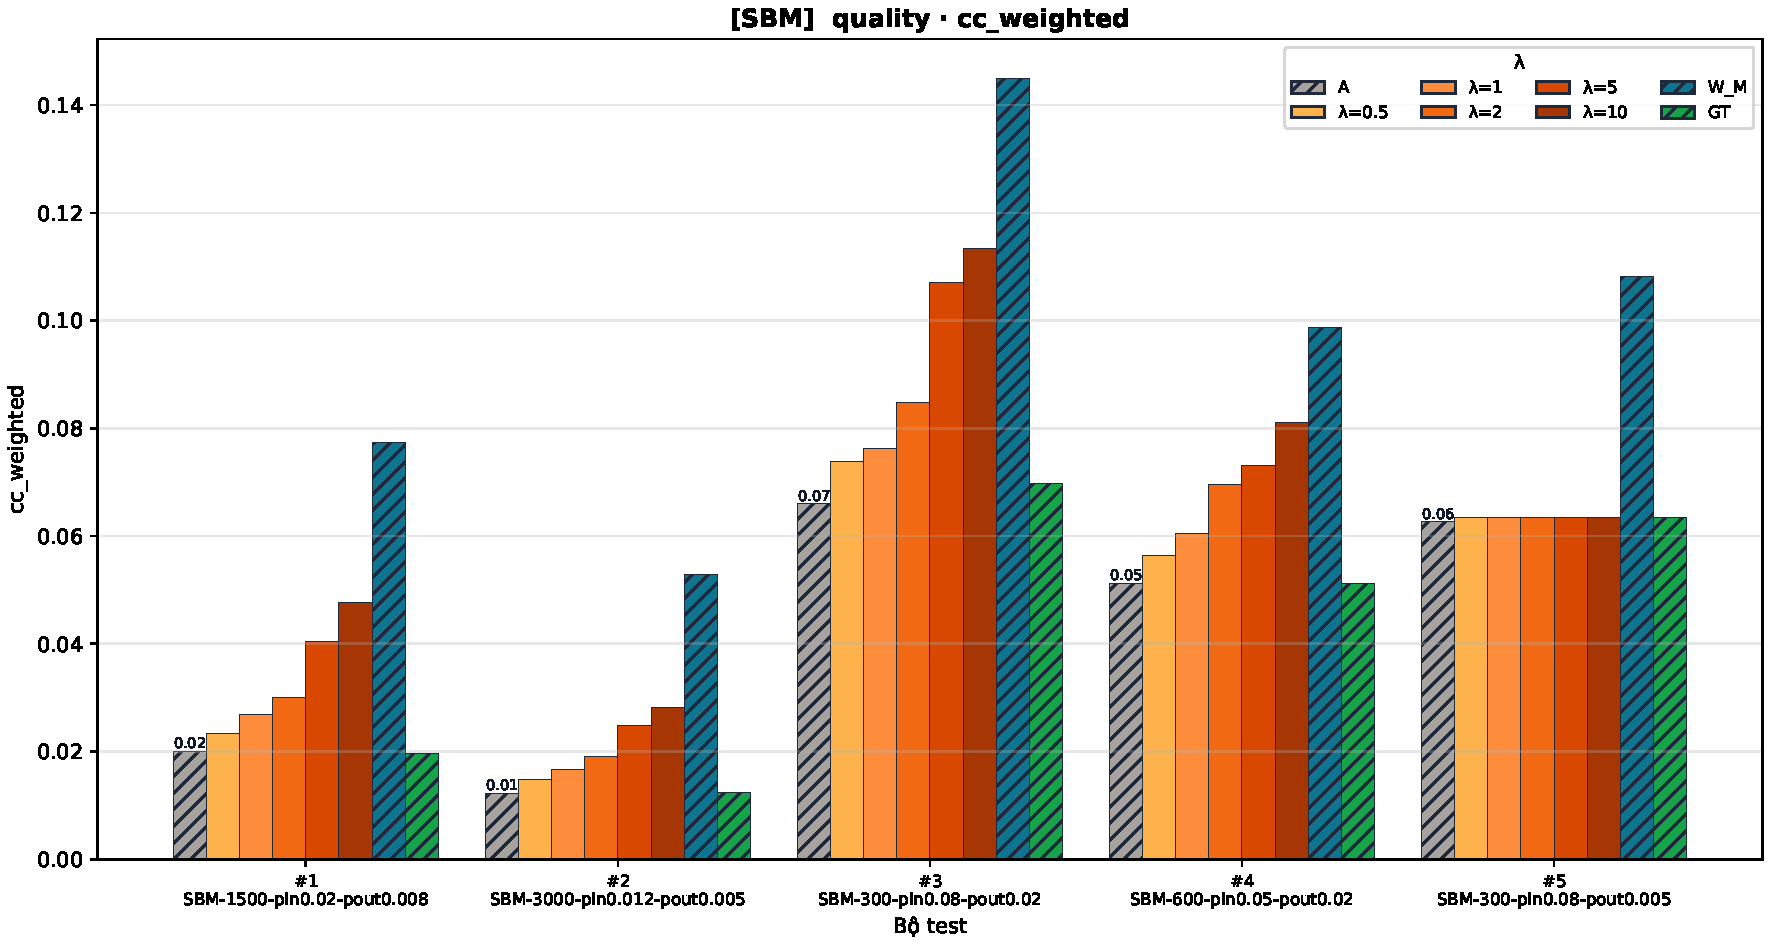
\includegraphics[width=\textwidth]{../main_result/SBM/charts/quality_cc_weighted.pdf}
    \caption{$\overline{\mathrm{CC}}_w$ trên năm bộ SBM theo $\lambda$.}
    \label{fig:sbm-cc-weighted}
\end{figure}

\begin{figure}[H]
    \centering
    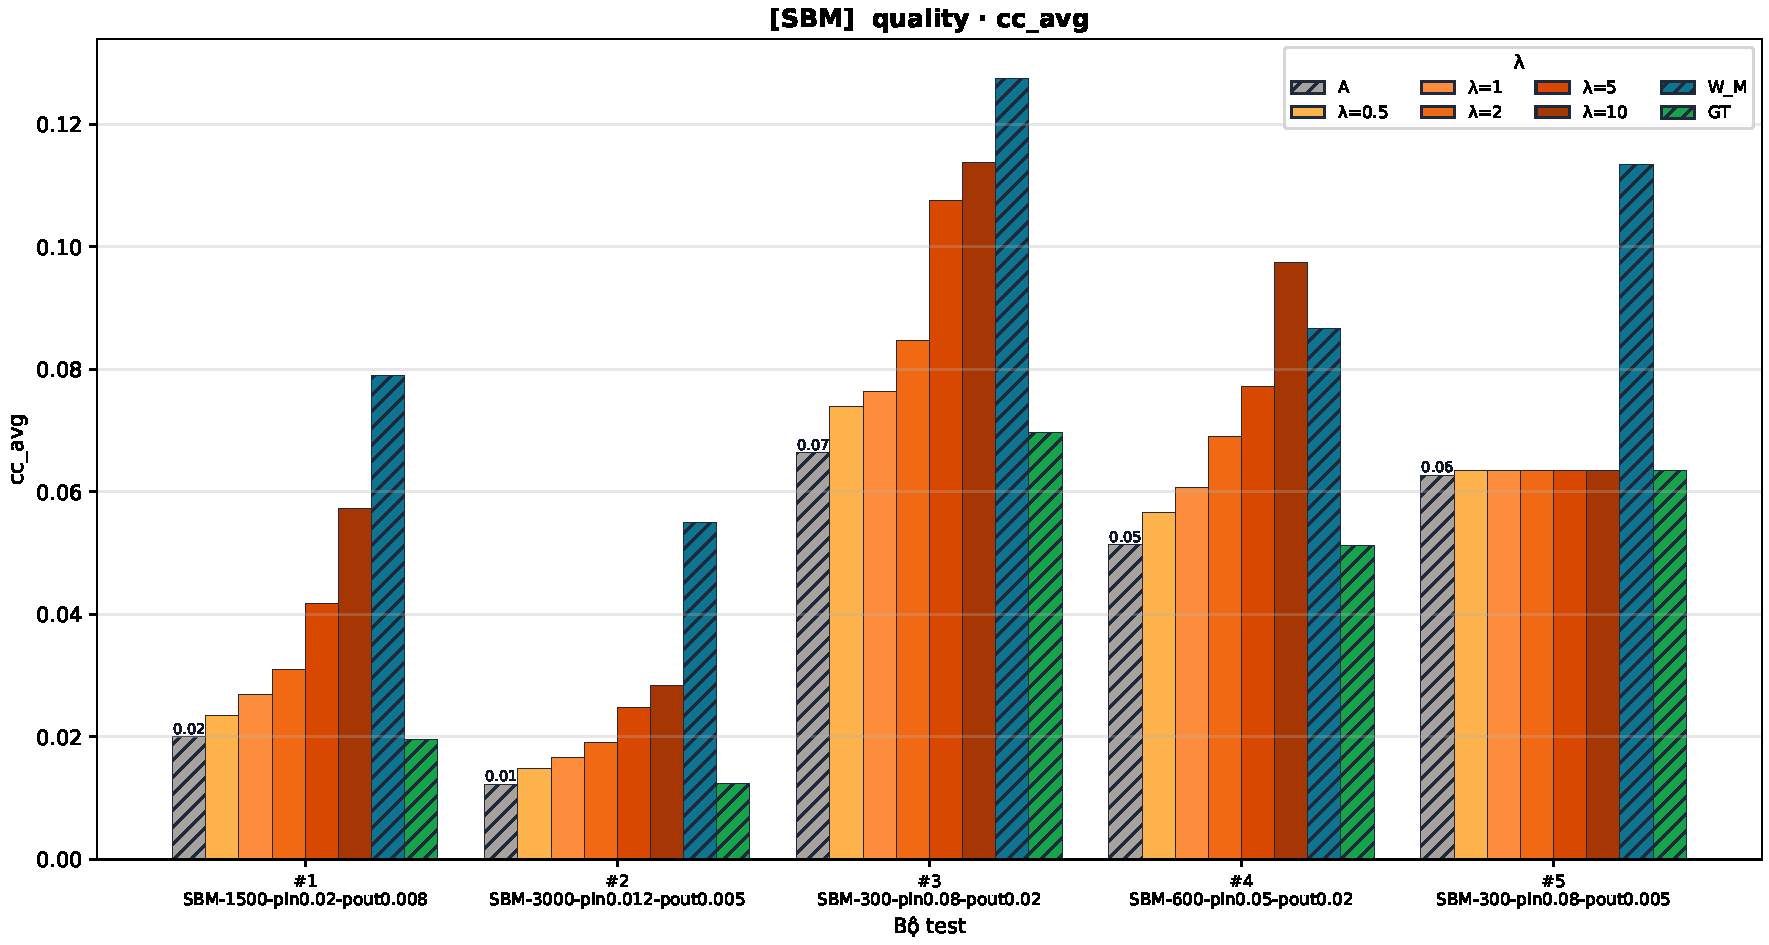
\includegraphics[width=\textwidth]{../main_result/SBM/charts/quality_cc_avg.pdf}
    \caption{$\overline{\mathrm{CC}}$ trên năm bộ SBM theo $\lambda$.}
    \label{fig:sbm-cc-avg}
\end{figure}

\textbf{Quan sát.} $cc_{\mathrm{global}} = 0{,}0128$ cho đồ thị nền của bộ SBM-1500-$p_{\mathrm{out}}0{,}008$ rất thấp, phù hợp với tính chất sinh cạnh độc lập theo cặp. Trên bộ này, $\overline{\mathrm{CC}}_w$ chuyển từ $0{,}0200$ tại $\lambda = 0$ lên $0{,}0773$ tại $W_M$, gấp khoảng sáu lần baseline. $\overline{\mathrm{CC}}$ cùng tăng đến $0{,}0791$ tại $W_M$. Cả hai đại lượng tăng đơn điệu theo $\lambda$ trên cả năm bộ test, ngược chiều biến thiên của $Q$ và NMI.

\textbf{Nhận xét.} Mức tăng tuyệt đối nhỏ ($\overline{\mathrm{CC}}_w$ tại đỉnh chỉ $0{,}0773$, thấp xa so với mức quan sát được trên LFR) phù hợp với việc SBM không sinh nhiều tam giác có nghĩa. Tỉ số $\overline{\mathrm{CC}}_w / cc_{\mathrm{global}}$ tăng chủ yếu vì baseline thấp, không phải vì thuật toán phát hiện cấu trúc tam giác đậm đặc. Sự đối lập về chiều giữa nhóm $\{\overline{\mathrm{CC}}, \overline{\mathrm{CC}}_w\}$ và nhóm $\{Q, \mathrm{NMI}\}$ mang ý nghĩa diễn giải quan trọng: dưới trọng số motif lớn, thuật toán gom được các tam giác về cùng cụm nhưng các cụm thu được lại không phản ánh phân hoạch chuẩn. Hệ quả phương pháp luận: $\overline{\mathrm{CC}}_w$, dù phản ánh đúng định nghĩa, không thể thay thế modularity hay NMI khi kiểm chứng tính đúng của phân hoạch trên SBM. Tương tự, $\overline{\mathrm{CC}}$ và $\overline{\mathrm{CC}}_w$ trùng nhau gần như chính xác, cho thấy SBM với $K = 3$ và kích thước cụm bằng nhau không có cụm nhỏ thiên lệch trung bình không trọng số.

% ............................................................
\subsection{Planted Partition}
\label{subsec:results-planted}

Planted Partition là trường hợp đặc biệt của SBM trong đó mọi cụm có cùng kích thước $s$ và mọi cặp khối dùng chung một cặp $(p_{\mathrm{in}}, p_{\mathrm{out}})$. Mức độ đối xứng cao khiến mô hình này thường được dùng làm baseline kiểm tra hành vi cơ bản của thuật toán. Khoá luận cố định $K = 5$ và quét $s \in \{40, 100, 200, 400\}$ với các cặp $(p_{\mathrm{in}}, p_{\mathrm{out}})$ tương ứng để bao quát các mức độ tách cộng đồng từ yếu đến rõ.

\subsubsection*{Modularity và NMI}

\begin{table}[H]
\centering
\caption{Bốn bộ test Planted có cải thiện modularity lớn nhất}
\label{tab:planted-top5}
\begin{tabular}{|l|c|c|c|c|c|c|}
\hline
\textbf{Bộ test} & $Q(0)$ & $\lambda{=}0{,}5$ & $\lambda{=}1$ & $\lambda{=}2$ & $\lambda{=}5$ & $\lambda^*$ \\ \hline
Planted-$s100$-$p_{\mathrm{in}}0{,}08$-$p_{\mathrm{out}}0{,}025$  & 0{,}1203 & \textbf{0{,}2185} & 0{,}2087 & 0{,}1937 & 0{,}1825 & $0{,}5$ \\ \hline
Planted-$s40$-$p_{\mathrm{in}}0{,}15$-$p_{\mathrm{out}}0{,}03$   & 0{,}2424 & \textbf{0{,}3164} & 0{,}3068 & 0{,}2862 & 0{,}2955 & $0{,}5$ \\ \hline
Planted-$s400$-$p_{\mathrm{in}}0{,}025$-$p_{\mathrm{out}}0{,}006$ & 0{,}2960 & \textbf{0{,}2974} & 0{,}2930 & 0{,}2774 & 0{,}2379 & $0{,}5$ \\ \hline
Planted-$s200$-$p_{\mathrm{in}}0{,}05$-$p_{\mathrm{out}}0{,}005$  & 0{,}5156 & \textbf{0{,}5156} & 0{,}5146 & 0{,}5107 & 0{,}5009 & $0{,}5$ \\ \hline
\end{tabular}
\end{table}

\begin{figure}[H]
    \centering
    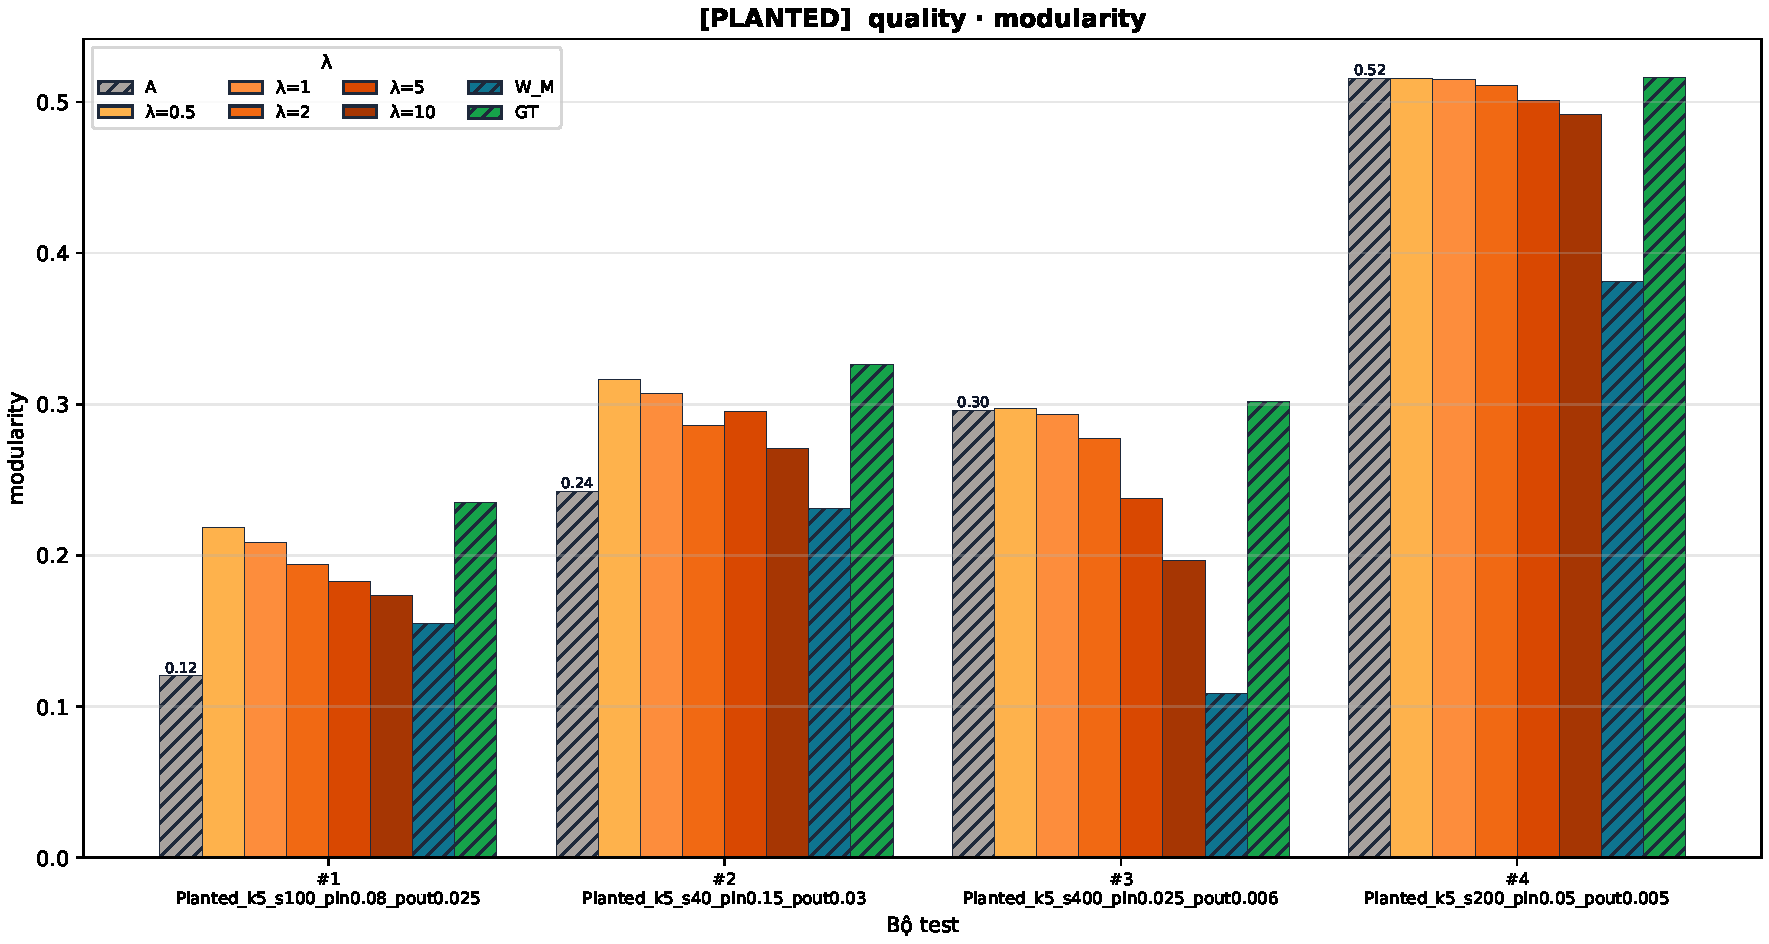
\includegraphics[width=\textwidth]{../main_result/PLANTED/charts/quality_modularity.pdf}
    \caption[Modularity $Q$ trên bốn bộ Planted Partition theo $\lambda$.]{Modularity $Q$ trên bốn bộ Planted Partition theo $\lambda$.}
    \label{fig:planted-modularity}
\end{figure}

\begin{figure}[H]
    \centering
    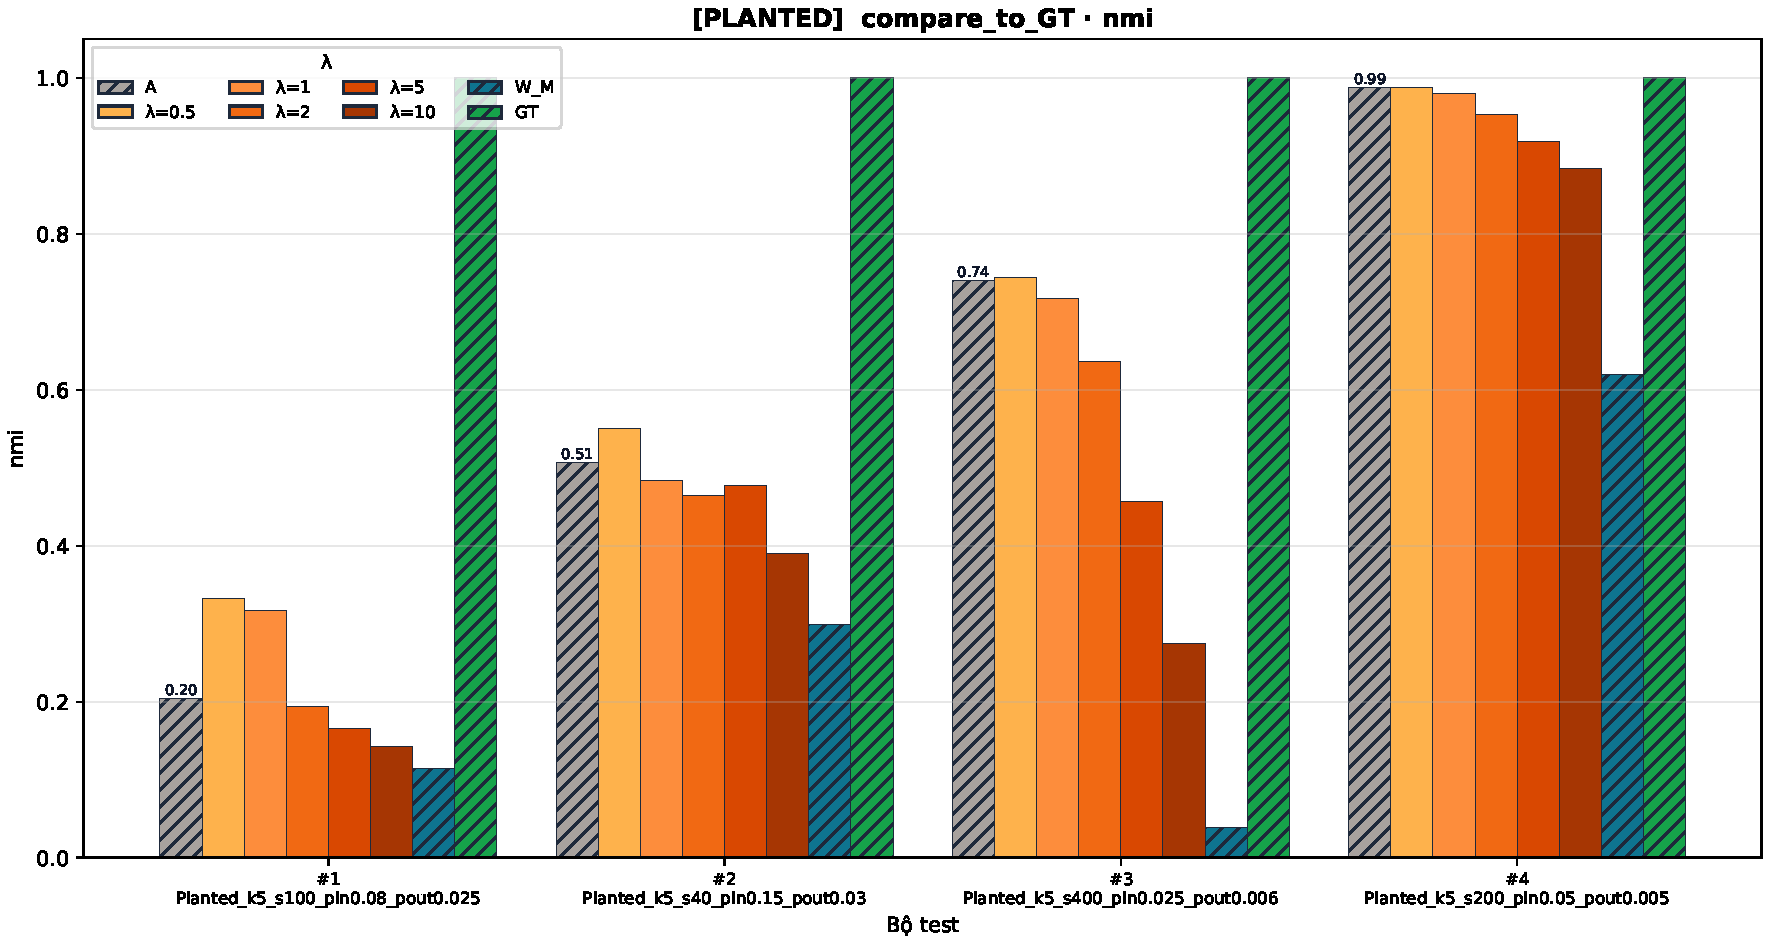
\includegraphics[width=\textwidth]{../main_result/PLANTED/charts/compare_to_GT_nmi.pdf}
    \caption{NMI so với phân hoạch chuẩn trên bốn bộ Planted Partition theo $\lambda$.}
    \label{fig:planted-nmi}
\end{figure}

\textbf{Quan sát.} $\lambda^* = 0{,}5$ trên cả bốn bộ test. Hai bộ có cộng đồng tách yếu cho $\Delta Q$ đáng kể ($+0{,}098$ và $+0{,}074$); hai bộ tách rõ gần như không cải thiện. NMI đạt đỉnh đồng thuận với modularity tại $\lambda = 0{,}5$ và giảm dần theo cùng nhịp khi $\lambda$ tăng.

\textbf{Nhận xét.} Pattern lặp lại nguyên vẹn từ SBM — điều dự kiến do Planted là trường hợp đặc biệt của SBM. Hiệu ứng bão hoà theo $Q(0)$ tỏ ra rõ rệt: khi cộng đồng đã tách rõ trong $A$, modularity ban đầu cao và phần thông tin còn lại để motif đóng góp gần như bằng không. Việc cộng đồng đối xứng, kích thước bằng nhau và xác suất sinh cạnh đồng nhất giữa các cặp khối làm cho tam giác trở thành đại lượng nhiễu thuần tuý theo nghĩa thống kê; do đó vai trò của $W^{(M)}$ chỉ dừng ở mức ổn định hoá phân cụm phổ, không bổ sung được tín hiệu cấu trúc riêng.

\subsubsection*{Hệ số phân cụm}

\begin{figure}[H]
    \centering
    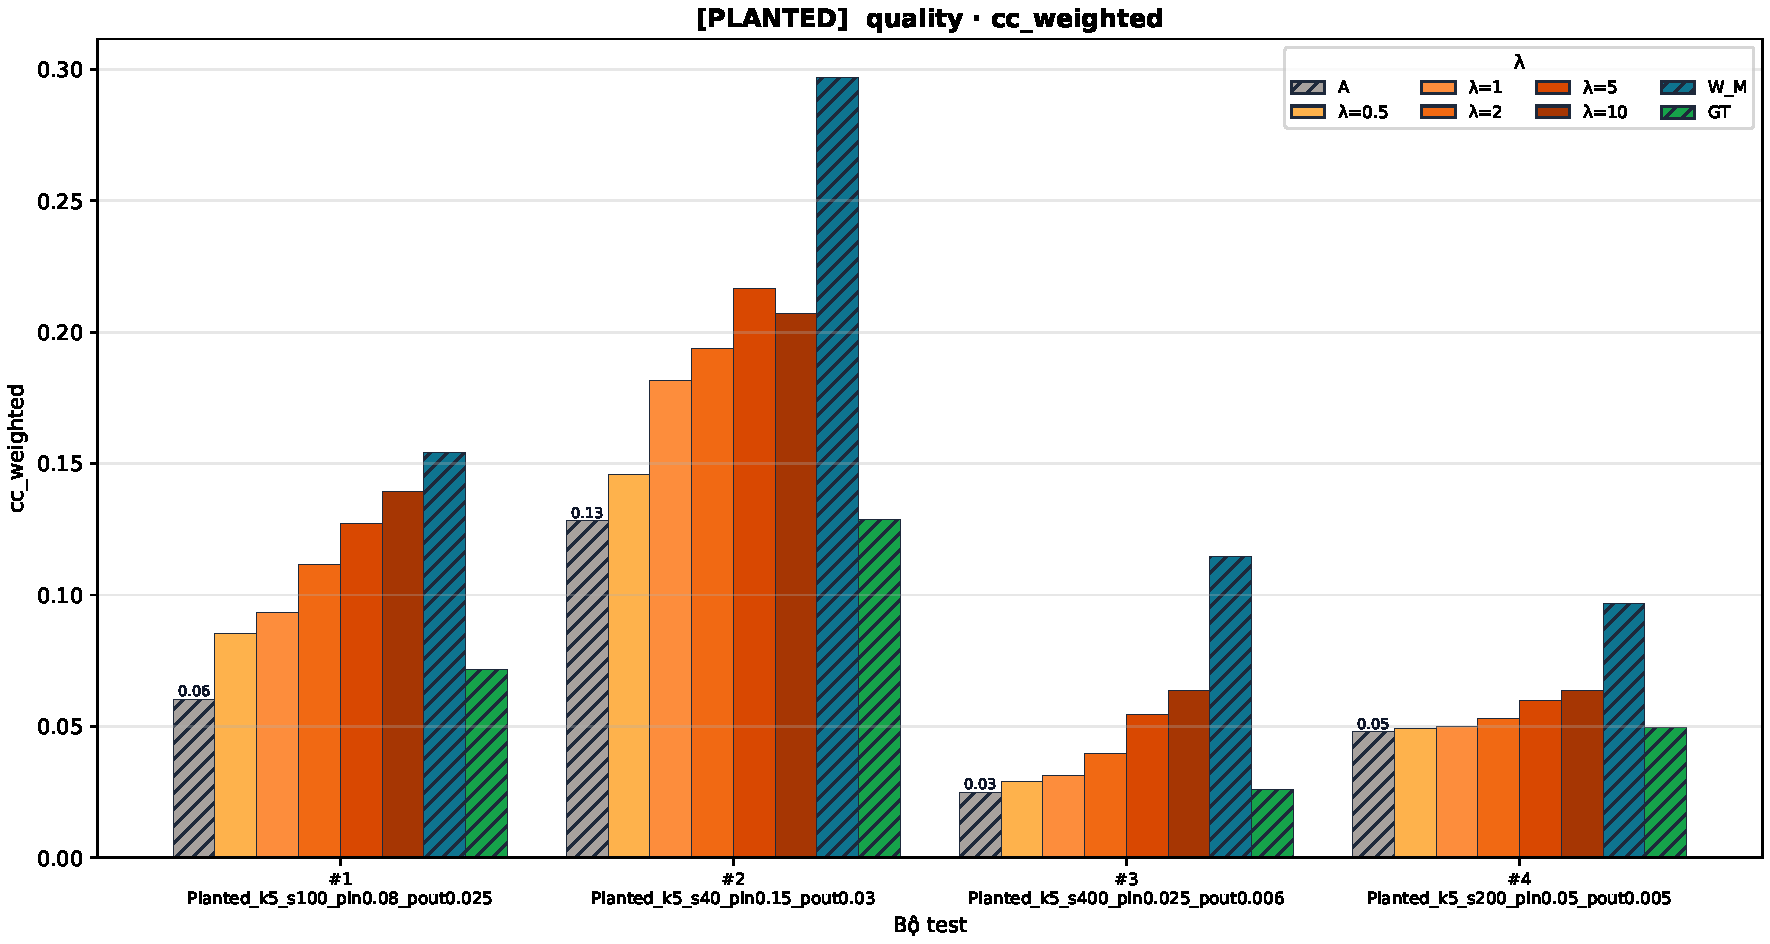
\includegraphics[width=\textwidth]{../main_result/PLANTED/charts/quality_cc_weighted.pdf}
    \caption{$\overline{\mathrm{CC}}_w$ trên bốn bộ Planted Partition theo $\lambda$.}
    \label{fig:planted-cc-weighted}
\end{figure}

\begin{figure}[H]
    \centering
    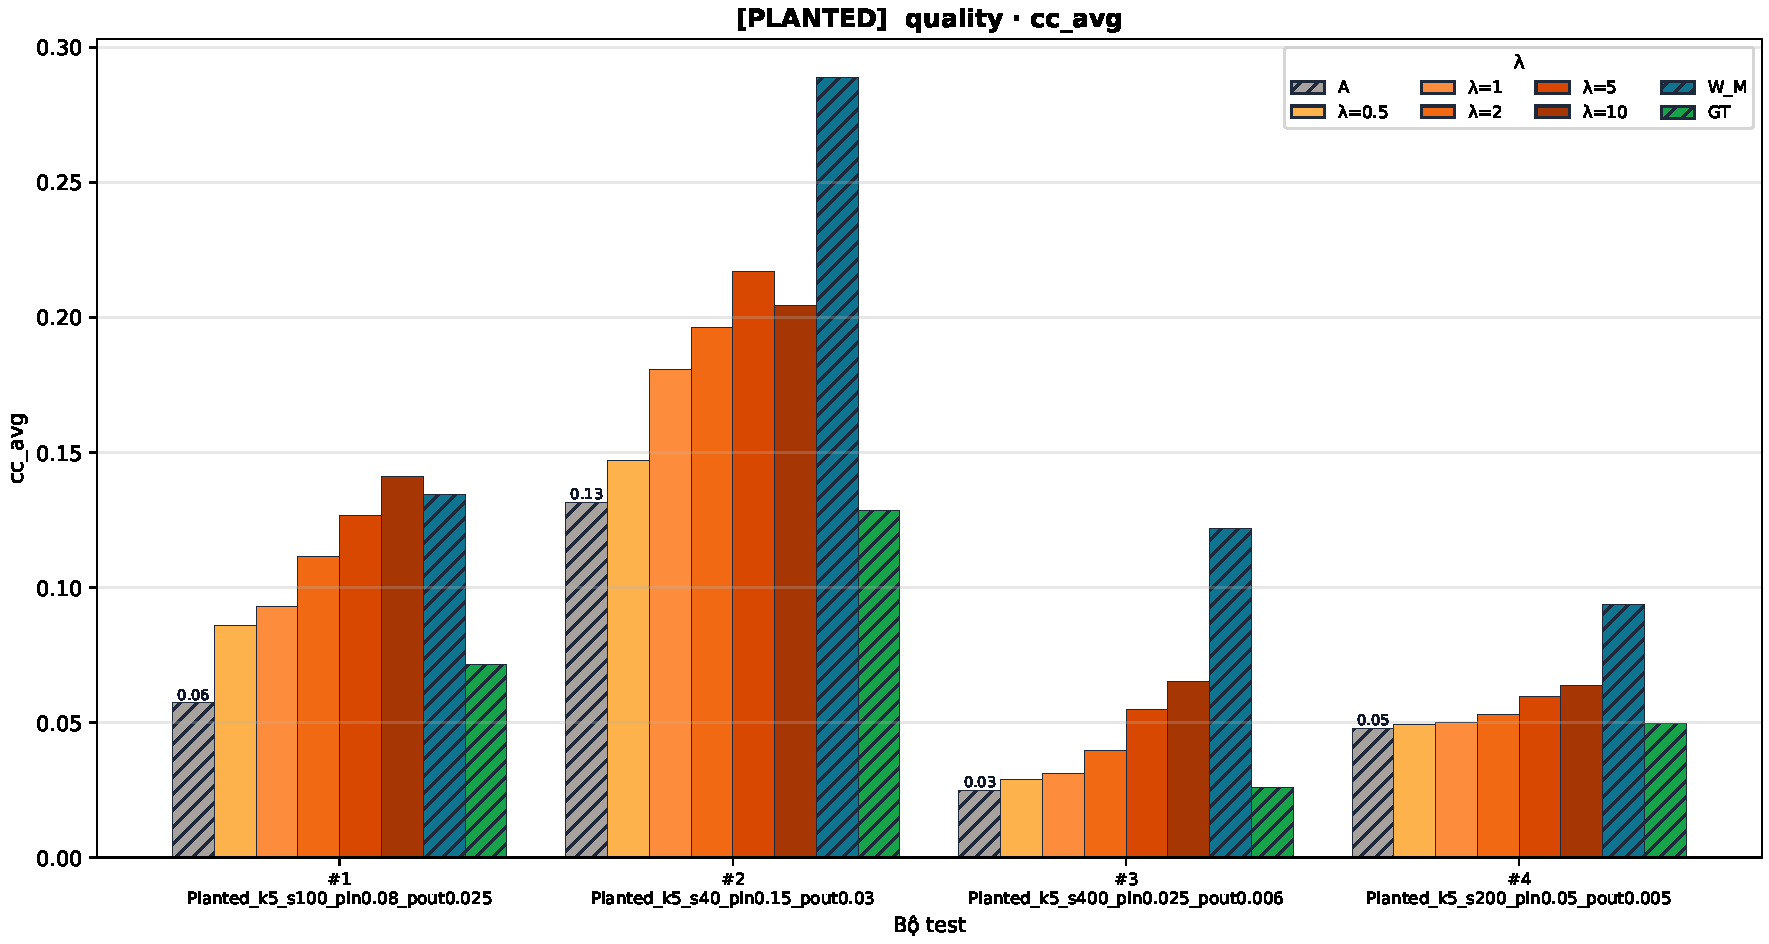
\includegraphics[width=\textwidth]{../main_result/PLANTED/charts/quality_cc_avg.pdf}
    \caption{$\overline{\mathrm{CC}}$ trên bốn bộ Planted Partition theo $\lambda$.}
    \label{fig:planted-cc-avg}
\end{figure}

\textbf{Quan sát.} $cc_{\mathrm{global}} = 0{,}0379$ cho đồ thị nền của bộ Planted-$s100$-$p_{\mathrm{in}}0{,}08$-$p_{\mathrm{out}}0{,}025$. $\overline{\mathrm{CC}}_w$ tăng từ $0{,}0604$ tại $\lambda = 0$ lên $0{,}1540$ tại $W_M$ (gấp khoảng bốn lần baseline), $\overline{\mathrm{CC}}$ đạt $0{,}1412$ tại $\lambda = 10$. Cả hai đại lượng tăng đơn điệu theo $\lambda$ trên cả bốn bộ test, trong khi $Q$ và NMI đỉnh tại $\lambda = 0{,}5$ rồi suy giảm.

\textbf{Nhận xét.} Pattern lặp lại nguyên vẹn từ SBM, điều dự kiến vì Planted là trường hợp đặc biệt của SBM. Khoảng cách hẹp giữa $\overline{\mathrm{CC}}$ và $\overline{\mathrm{CC}}_w$ là hệ quả trực tiếp của cơ chế sinh: tất cả cụm có cùng kích thước nên không có cụm nhỏ kéo trung bình không trọng số lên cao. Sự lặp lại pattern phân kỳ giữa $\{\overline{\mathrm{CC}}, \overline{\mathrm{CC}}_w\}$ và $\{Q, \mathrm{NMI}\}$ trên hai mô hình SBM và Planted khẳng định một nguyên lý chung: trên đồ thị sinh ngẫu nhiên đối xứng, mật độ tam giác nội cụm và tính đúng của phân hoạch là hai mục tiêu có thể tách biệt; tối ưu một trong hai không tự động kéo theo cải thiện đại lượng còn lại.

% ............................................................
\subsection{Gaussian Random Partition Graph}
\label{subsec:results-grpg}

Gaussian Random Partition Graph nằm giữa Planted Partition và LFR về mức độ đa dạng kích thước cụm. Kích thước mỗi cụm được lấy mẫu từ phân bố Gaussian $\mathcal{N}(s, s/v)$ với $s$ là kích thước trung bình và $v$ là tham số hình dạng kiểm soát phương sai; cạnh sau đó được sinh theo cơ chế Planted Partition trên tập cụm thu được. Khoá luận quét $n \in \{200, 500, 2000\}$ với các cặp $(p_{\mathrm{in}}, p_{\mathrm{out}})$ và $s$ tương ứng để bao quát các mức độ tách cộng đồng từ yếu đến rõ.

\subsubsection*{Modularity và NMI}

\begin{table}[H]
\centering
\caption{Năm bộ test GRPG có cải thiện modularity lớn nhất}
\label{tab:grpg-top5}
\begin{tabular}{|l|c|c|c|c|c|c|}
\hline
\textbf{Bộ test} & $Q(0)$ & $\lambda{=}0{,}5$ & $\lambda{=}1$ & $\lambda{=}2$ & $\lambda{=}5$ & $\lambda^*$ \\ \hline
GRPG-2000-$p_{\mathrm{out}}0{,}006$ & 0{,}1165 & 0{,}2004 & \textbf{0{,}2005} & 0{,}1887 & 0{,}1678 & $1{,}0$ \\ \hline
GRPG-500-$p_{\mathrm{out}}0{,}008$  & 0{,}4240 & \textbf{0{,}4753} & 0{,}4728 & 0{,}4668 & 0{,}4590 & $0{,}5$ \\ \hline
GRPG-500-$p_{\mathrm{out}}0{,}015$  & 0{,}2914 & \textbf{0{,}3400} & 0{,}3307 & 0{,}3113 & 0{,}3026 & $0{,}5$ \\ \hline
GRPG-2000-$p_{\mathrm{out}}0{,}001$ & 0{,}6209 & \textbf{0{,}6611} & 0{,}6196 & 0{,}6600 & 0{,}6573 & $0{,}5$ \\ \hline
GRPG-200-$p_{\mathrm{out}}0{,}03$   & 0{,}3593 & \textbf{0{,}3606} & 0{,}3572 & 0{,}3523 & 0{,}3436 & $0{,}5$ \\ \hline
\end{tabular}
\end{table}

\begin{figure}[H]
    \centering
    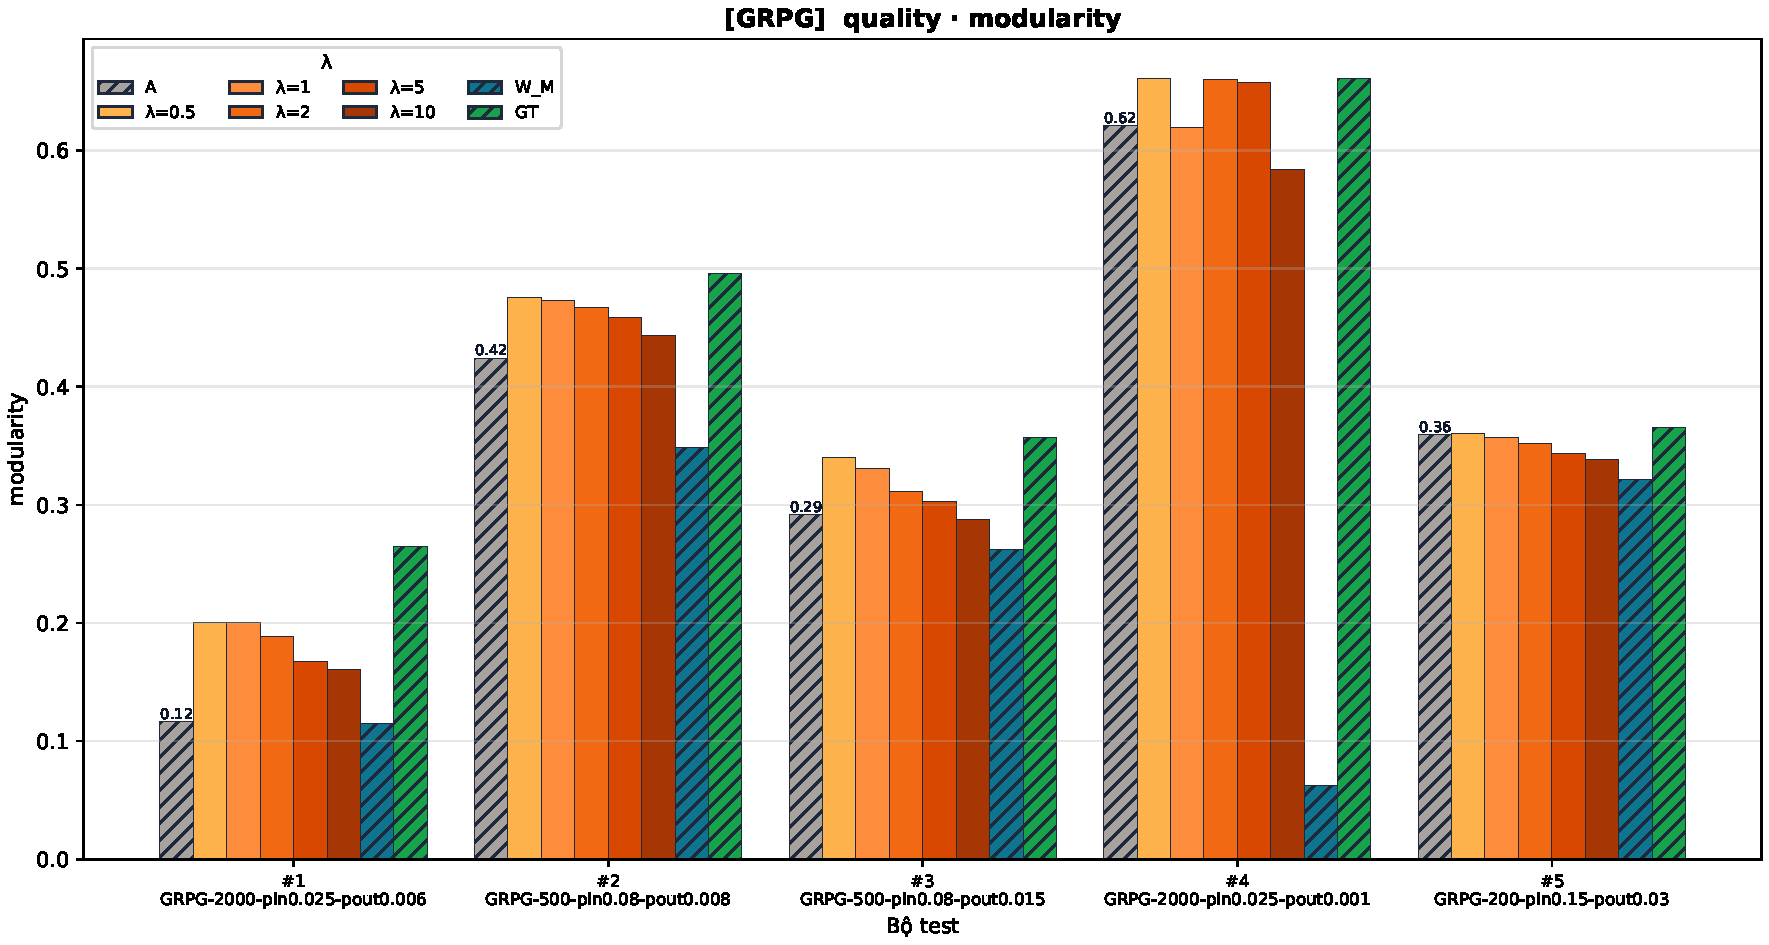
\includegraphics[width=\textwidth]{../main_result/GRPG/charts/quality_modularity.pdf}
    \caption[Modularity $Q$ trên năm bộ GRPG theo $\lambda$.]{Modularity $Q$ trên năm bộ GRPG theo $\lambda$.}
    \label{fig:grpg-modularity}
\end{figure}

\begin{figure}[H]
    \centering
    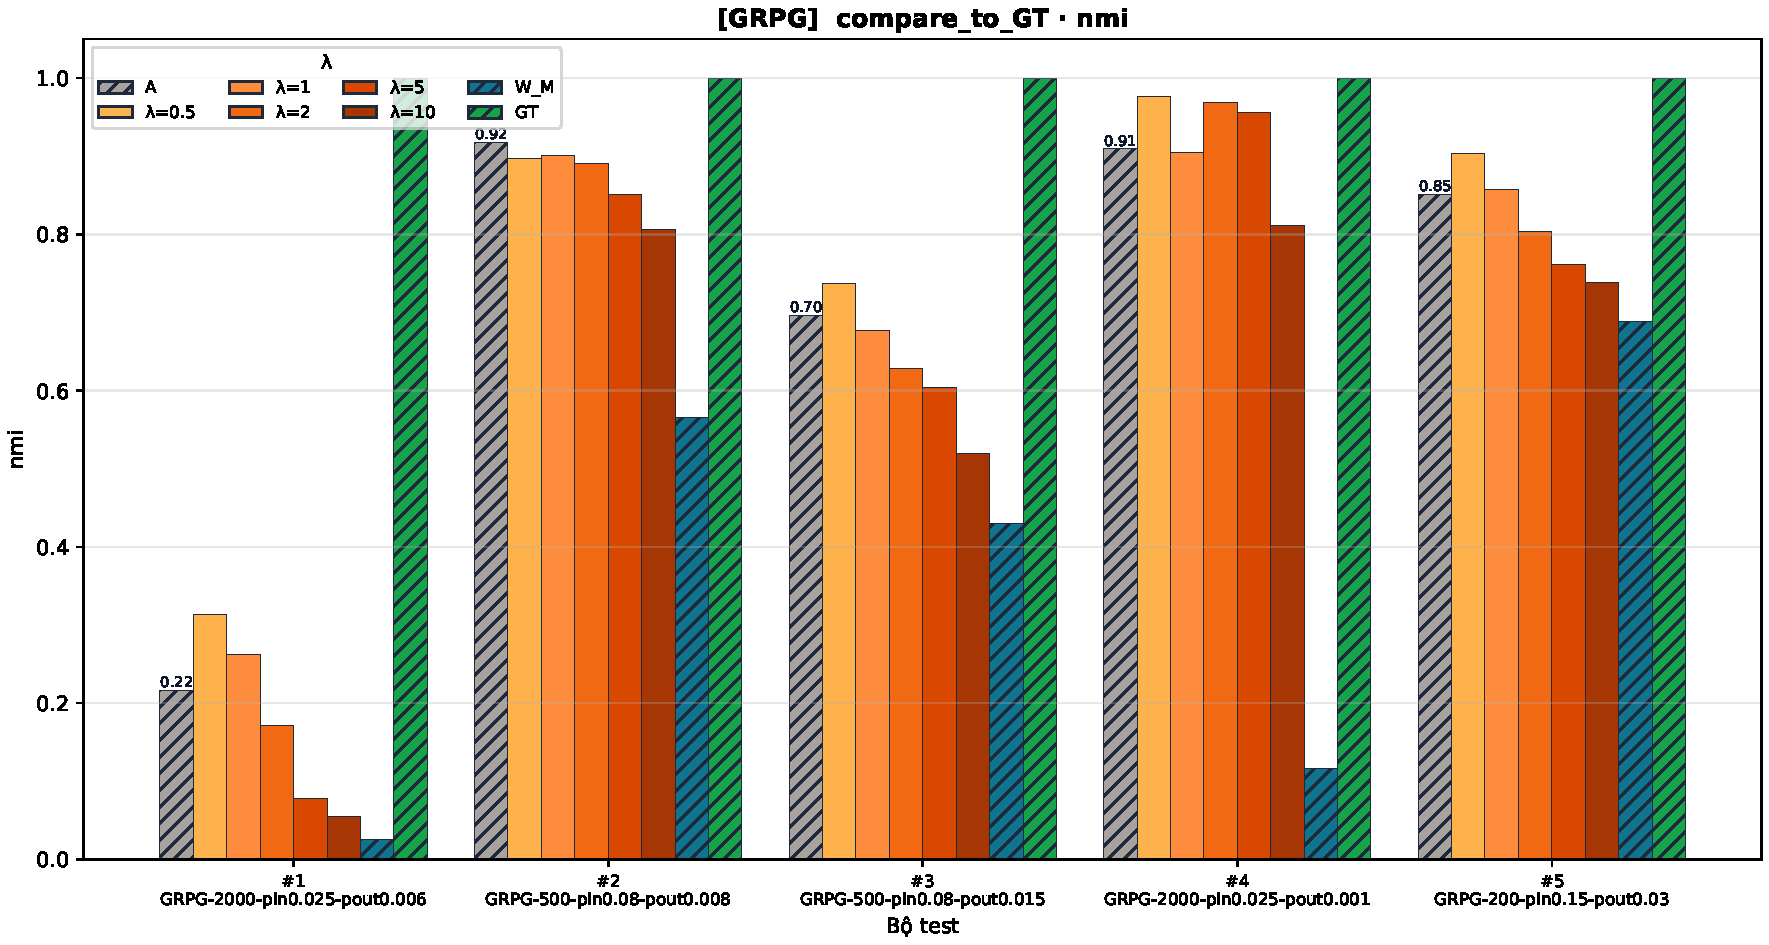
\includegraphics[width=\textwidth]{../main_result/GRPG/charts/compare_to_GT_nmi.pdf}
    \caption{NMI so với phân hoạch chuẩn trên năm bộ GRPG theo $\lambda$.}
    \label{fig:grpg-nmi}
\end{figure}

\textbf{Quan sát.} $\lambda^*$ luôn thuộc $\{0{,}5, 1\}$, nhưng biên độ cải thiện vượt Planted: bộ GRPG-2000-$p_{\mathrm{out}}0{,}006$ cho $\Delta Q = +0{,}0840$, cùng cấp độ với các bộ LFR khó nhất. NMI đạt đỉnh tại $\lambda = 0{,}5$, sớm hơn modularity (đỉnh tại $\lambda = 1$) một bước.

\textbf{Nhận xét.} GRPG cho hành vi trung gian giữa Planted và LFR. Sự đa dạng về kích thước cụm sinh ra từ phân bố Gaussian dường như mở rộng phạm vi $\lambda$ mà motif còn đóng góp tích cực, đẩy biên độ cải thiện vượt Planted dù chưa đủ để $\lambda^*$ vượt khỏi vùng nhỏ. Sự lệch pha một bước giữa đỉnh NMI và đỉnh modularity là cảnh báo phương pháp luận: ngay trong vùng cải thiện, phân hoạch tối ưu theo modularity đã bắt đầu rời khỏi phân hoạch chuẩn. Việc dựa hoàn toàn vào modularity để chọn $\lambda^*$ có thể dẫn đến phân hoạch lệch khỏi ground truth dù $\Delta Q$ vẫn dương.

\subsubsection*{Hệ số phân cụm}

\begin{figure}[H]
    \centering
    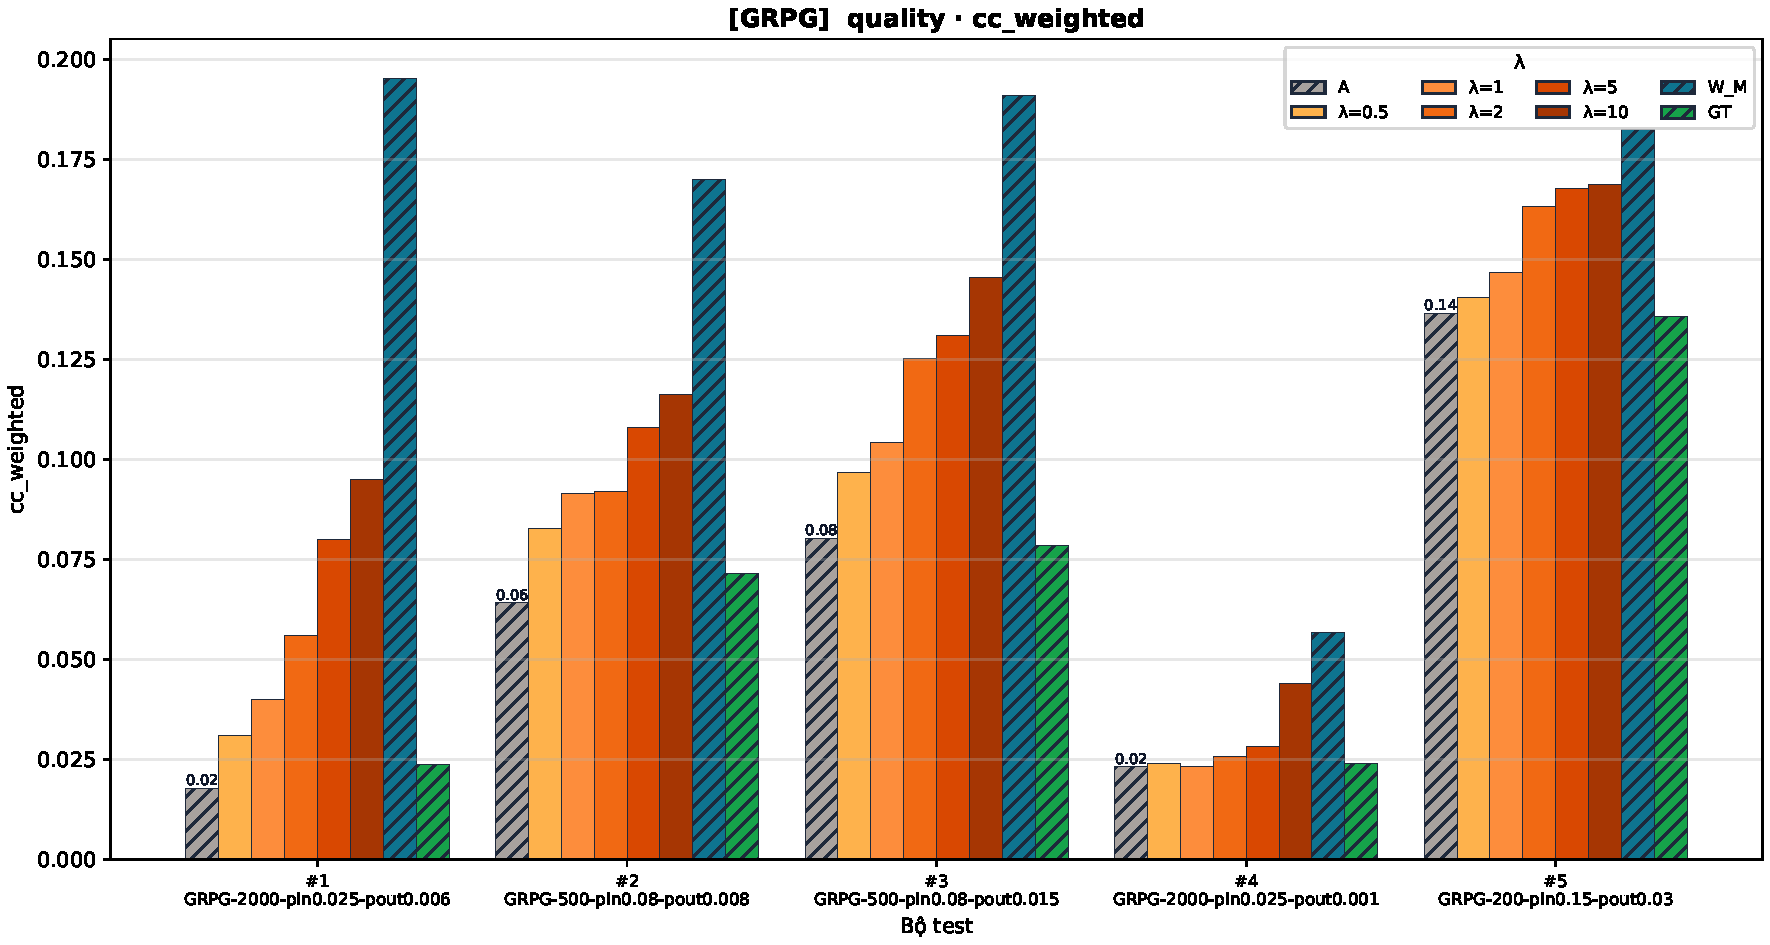
\includegraphics[width=\textwidth]{../main_result/GRPG/charts/quality_cc_weighted.pdf}
    \caption{$\overline{\mathrm{CC}}_w$ trên năm bộ GRPG theo $\lambda$.}
    \label{fig:grpg-cc-weighted}
\end{figure}

\begin{figure}[H]
    \centering
    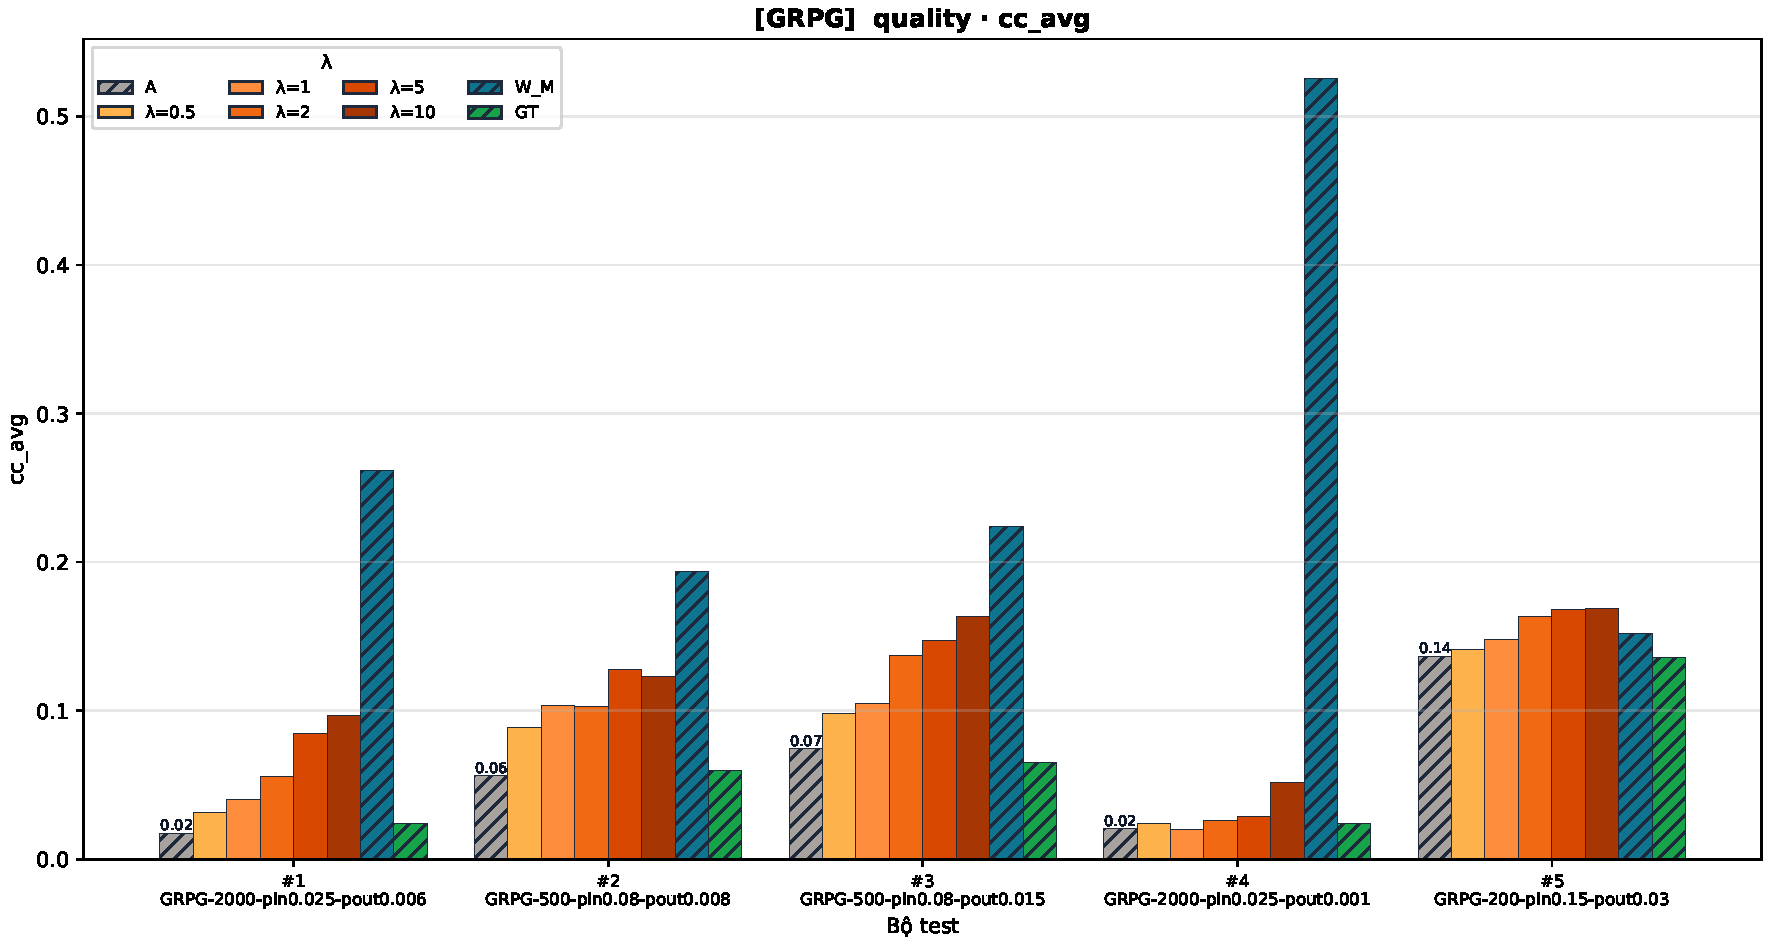
\includegraphics[width=\textwidth]{../main_result/GRPG/charts/quality_cc_avg.pdf}
    \caption{$\overline{\mathrm{CC}}$ trên năm bộ GRPG theo $\lambda$.}
    \label{fig:grpg-cc-avg}
\end{figure}

\textbf{Quan sát.} $cc_{\mathrm{global}} = 0{,}0104$ cho đồ thị nền của bộ GRPG-2000-$p_{\mathrm{out}}0{,}006$, ở mức rất thấp tương tự SBM. Trên bộ này, $\overline{\mathrm{CC}}_w$ tăng từ $0{,}0178$ tại $\lambda = 0$ lên $0{,}1953$ tại $W_M$, gấp khoảng mười một lần baseline. $\overline{\mathrm{CC}}$ đạt $0{,}2617$ tại $W_M$, cách $\overline{\mathrm{CC}}_w$ một khoảng đáng kể.

\textbf{Nhận xét.} Mức tăng tuyệt đối của $\overline{\mathrm{CC}}_w$ vượt trội so với SBM và Planted, phản ánh khả năng thuật toán cô lập các vùng tam giác đậm đặc khi phân bố kích thước cụm đa dạng. Khoảng cách rõ rệt giữa $\overline{\mathrm{CC}}$ và $\overline{\mathrm{CC}}_w$ tại $W_M$ là đặc trưng của GRPG: phân bố Gaussian sinh ra một số cụm kích thước nhỏ với hệ số phân cụm cao trên đơn vị đỉnh, làm thiên lệch trung bình không trọng số lên cao. Đây là minh hoạ thực nghiệm rõ nhất cho lý do khoá luận chọn $\overline{\mathrm{CC}}_w$ làm chỉ số chính (Định nghĩa~\ref{def:cc-cluster}): trên các đồ thị có kích thước cụm đa dạng, $\overline{\mathrm{CC}}$ có thể đánh giá quá lạc quan do hiệu ứng cụm nhỏ. Mặc dù vậy, pattern cốt lõi vẫn được giữ — cực đại của $\overline{\mathrm{CC}}_w$ không trùng cực đại của modularity, khẳng định tách biệt giữa hai mục tiêu trên lớp đồ thị sinh ngẫu nhiên đối xứng.

% ============================================================
\section{Đồ thị mạng xã hội thật}
\label{sec:results-real}

Mười một đồ thị thật được khảo sát với $\lambda \in \{0,\ 1,\ 5,\ 10,\ W_M\}$ và $K$ quét trong $\{50, 100, 200, 300, 400, 500\}$. Mỗi đồ thị có ý nghĩa đỉnh và cạnh riêng, dẫn đến đặc tính cấu trúc khác nhau. Bảng~\ref{tab:real-summary} tổng hợp bộ test có $\Delta Q$ cao nhất cho mỗi đồ thị, sau đó từng đồ thị được trình bày kèm biểu đồ chi tiết.

\begin{table}[H]
\centering
\small
\caption{Tổng hợp kết quả trên mười đồ thị mạng xã hội thật}
\label{tab:real-summary}
\begin{tabular}{|l|r|r|c|c|c|r|}
\hline
\textbf{Đồ thị} & $n$ & $m$ & $cc_{\mathrm{global}}$ & $K^*$ & $\lambda^*$ & $\Delta Q$ \\ \hline
musae\_DE\_edges    & 9{,}498   & 153{,}138 & 0{,}2009 & 50  & $W_M$ & $+0{,}1156$ \\ \hline
musae\_ES\_edges    & 4{,}648   & 59{,}382  & 0{,}2225 & 50  & $1{,}0$  & $+0{,}0902$ \\ \hline
lastfm\_asia\_edges & 7{,}624   & 27{,}806  & 0{,}2194 & 500 & $10{,}0$ & $+0{,}0815$ \\ \hline
Email-Enron         & 33{,}696  & 180{,}811 & 0{,}5092 & 300 & $5{,}0$  & $+0{,}0640$ \\ \hline
facebook\_combined  & 4{,}039   & 88{,}234  & 0{,}6055 & 500 & $5{,}0$  & $+0{,}0519$ \\ \hline
CA-GrQc             & 4{,}158   & 13{,}422  & 0{,}5569 & 500 & $5{,}0$  & $+0{,}0476$ \\ \hline
CA-AstroPh          & 17{,}903  & 196{,}972 & 0{,}6328 & 50  & $5{,}0$  & $+0{,}0421$ \\ \hline
CA-CondMat          & 21{,}363  & 91{,}286  & 0{,}6417 & 50  & $5{,}0$  & $+0{,}0316$ \\ \hline
CA-HepTh            & 8{,}638   & 24{,}806  & 0{,}4816 & 50  & $5{,}0$  & $+0{,}0250$ \\ \hline
musae\_facebook\_edges & 22{,}470 & 170{,}823 & 0{,}3597 & 500 & $5{,}0$ & $+0{,}0202$ \\ \hline
\end{tabular}
\end{table}

% ............................................................
\subsection*{musae\_DE}

Đỉnh là một streamer Twitch người Đức, cạnh nối hai streamer cùng chia sẻ người theo dõi. Cộng đồng có nghĩa là nhóm streamer cùng phân khúc khán giả. Hệ số phân cụm toàn cục $cc_{\mathrm{global}} = 0{,}2009$ ở mức trung bình.

\textbf{Modularity.}
\begin{figure}[H]
    \centering
    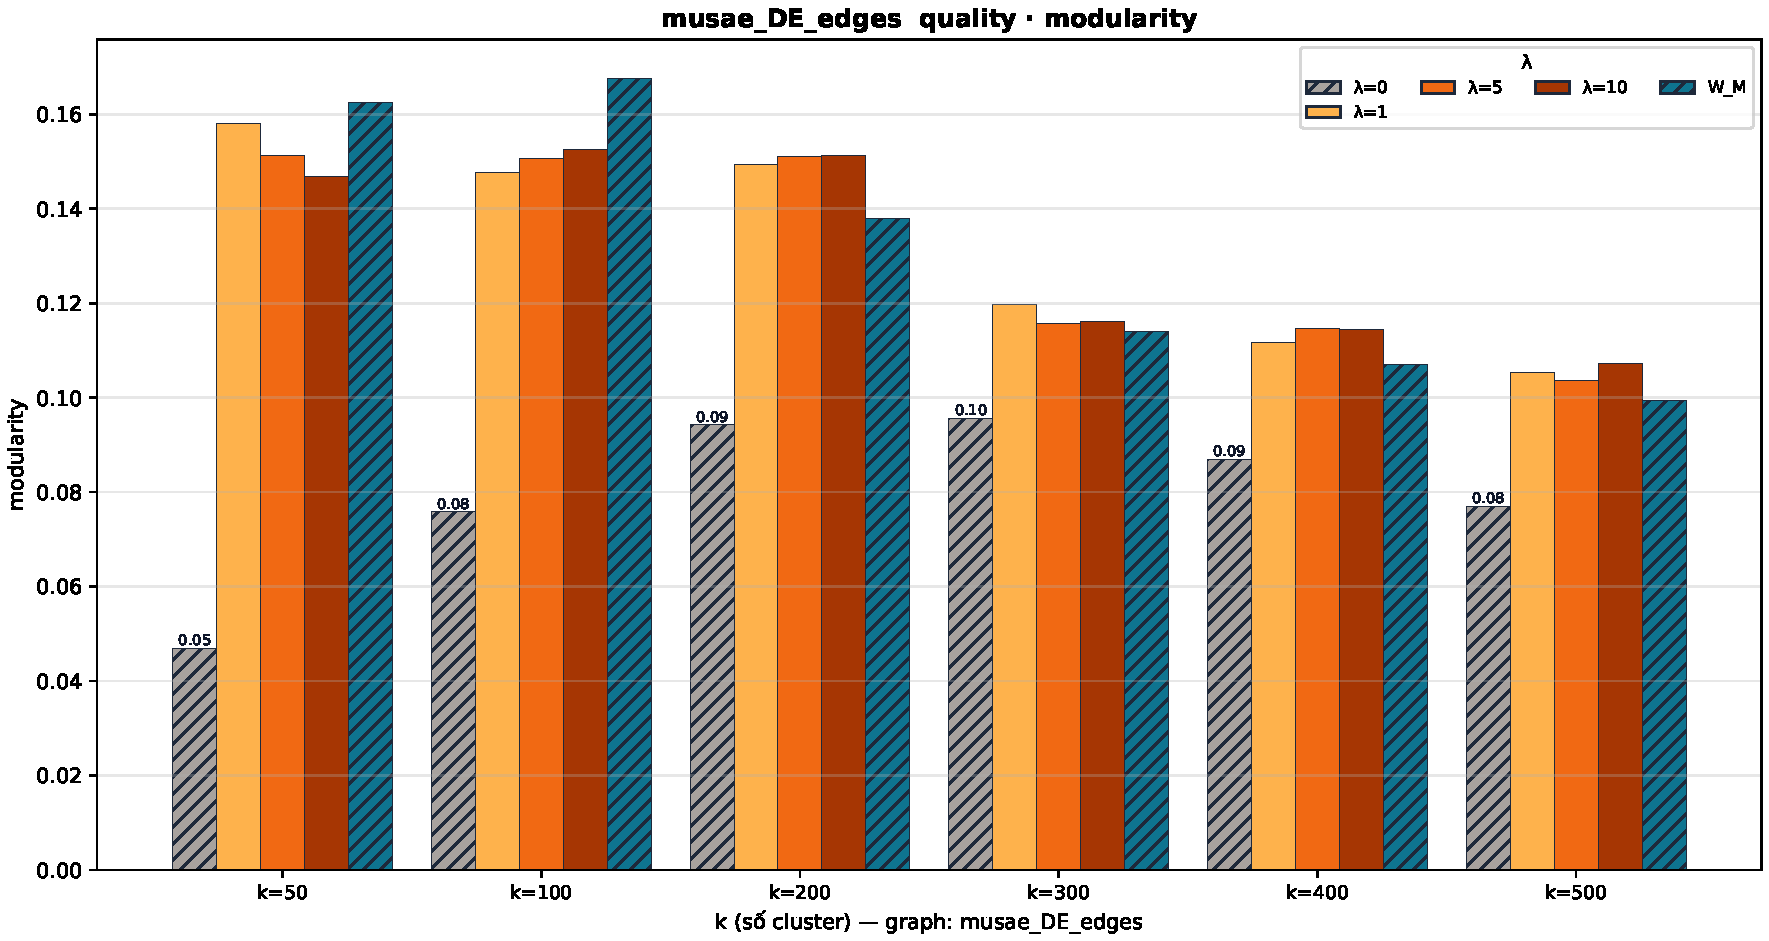
\includegraphics[width=\textwidth]{../main_result/REAL/musae_DE_edges/charts/quality_modularity.pdf}
    \caption{Modularity $Q$ trên musae\_DE theo $\lambda$ và $K$.}
    \label{fig:real-musae-de}
\end{figure}

$Q(0)$ rất thấp trên mọi $K$ (chỉ trong khoảng $0{,}05$--$0{,}10$). Ma trận hỗn hợp đẩy $Q$ lên gấp hai đến ba lần, mạnh nhất tại $K = 50$ với $\Delta Q = +0{,}1156$ và $\lambda^* = W_M$. Đây là trường hợp $Q(0)$ thấp điển hình: phân cụm phổ trên $A$ thuần không tìm được phân hoạch tốt, trọng số motif lớn tạo ra cải thiện rõ rệt.

\textbf{Hệ số phân cụm.}
\begin{figure}[H]
    \centering
    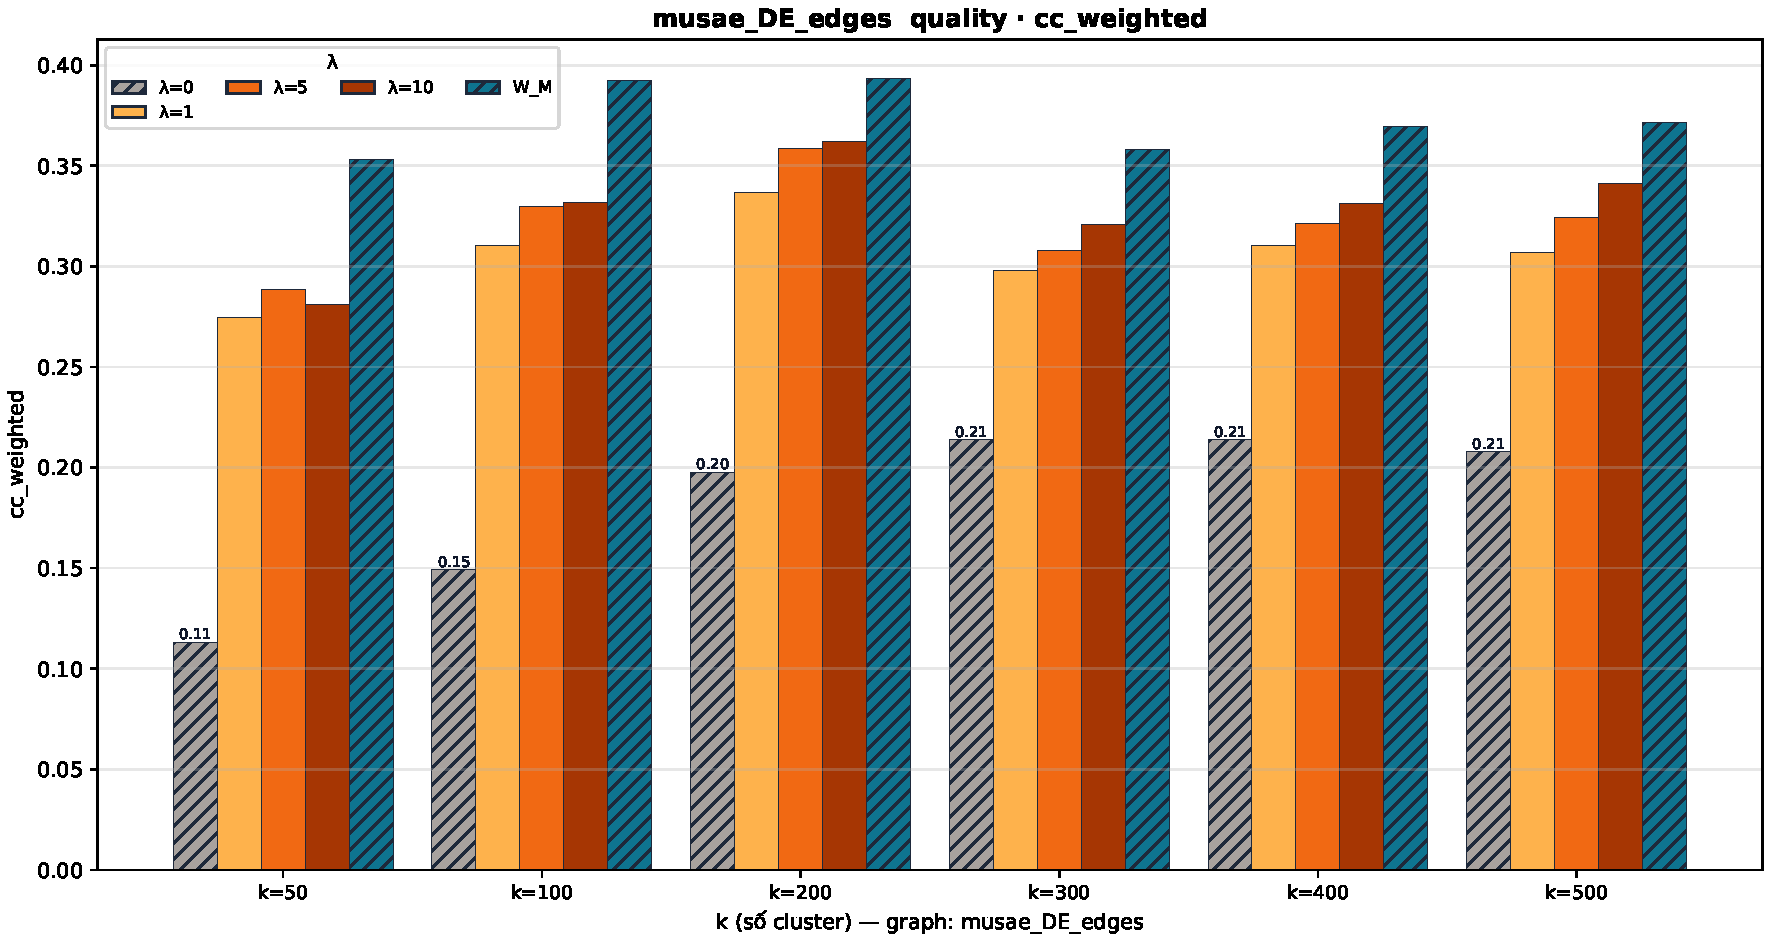
\includegraphics[width=\textwidth]{../main_result/REAL/musae_DE_edges/charts/quality_cc_weighted.pdf}
    \caption{$\overline{\mathrm{CC}}_w$ trên musae\_DE theo $\lambda$ và $K$.}
    \label{fig:real-cc-musae-de}
\end{figure}

\begin{figure}[H]
    \centering
    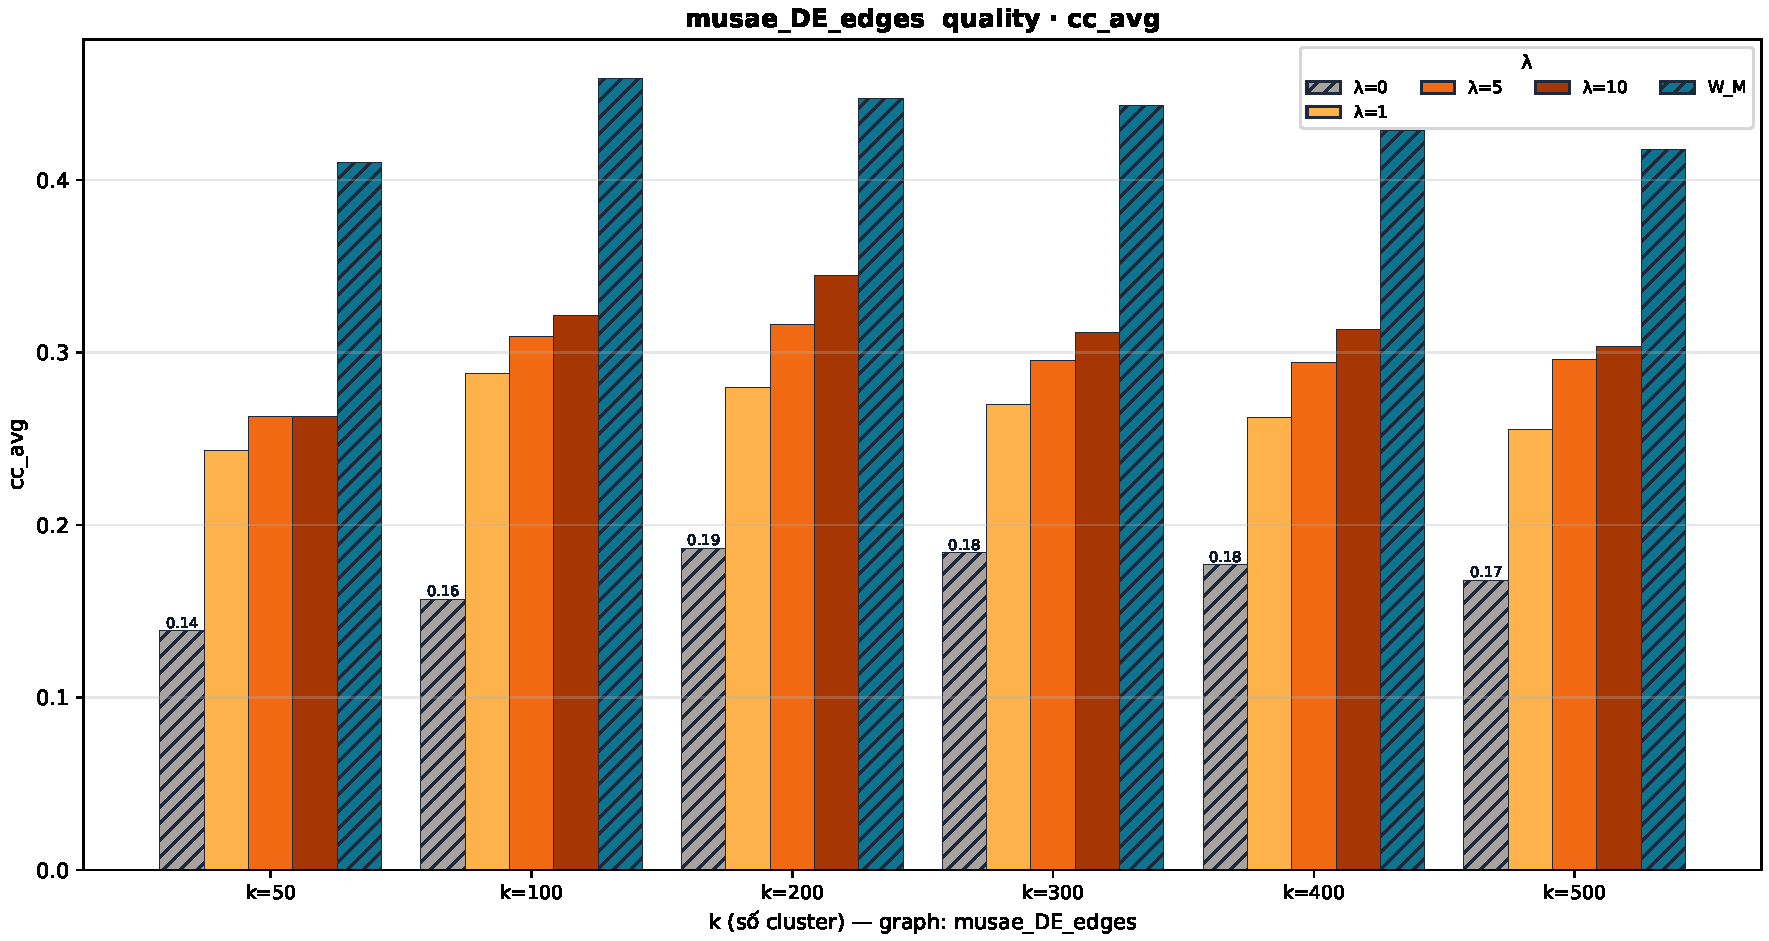
\includegraphics[width=\textwidth]{../main_result/REAL/musae_DE_edges/charts/quality_cc_avg.pdf}
    \caption{$\overline{\mathrm{CC}}$ trên musae\_DE theo $\lambda$ và $K$.}
    \label{fig:real-ccavg-musae-de}
\end{figure}

Tại $K = 50$, $\overline{\mathrm{CC}}_w(0) = 0{,}1132$ thấp hơn cả $cc_{\mathrm{global}}$, nghĩa là phân cụm phổ trên $A$ không gom được tam giác có sẵn vào trong cụm. Khi $\lambda$ chuyển về $W_M$, $\overline{\mathrm{CC}}_w$ đạt $0{,}3531$, gấp ba lần và vượt baseline $cc_{\mathrm{global}}$. $\overline{\mathrm{CC}}$ cũng tăng lên $0{,}4103$ tại $W_M$, bật từ $0{,}2630$ tại $\lambda = 10$ (tăng $0{,}15$ chỉ qua một bước sang $W_M$); $\overline{\mathrm{CC}}_w$ trong cùng đoạn chỉ tăng từ $0{,}2810$ lên $0{,}3531$, độ tăng nhỏ hơn rõ rệt. Điều này phù hợp với nhận định ở Định nghĩa~\ref{def:cc-cluster}: việc bỏ ma trận kề $A$ tạo ra một số cụm rất nhỏ với $\mathrm{CC}$ cục bộ cao, đẩy $\overline{\mathrm{CC}}$ lên trong khi $\overline{\mathrm{CC}}_w$ vẫn phản ánh trung thực kích thước cụm trung bình.

\textbf{Kết luận.} musae\_DE đại diện cho lớp đồ thị xã hội với triadic closure mạnh nhưng cộng đồng được mã hoá ẩn trong cấu trúc tam giác, không thể phát hiện chỉ qua cạnh. Trọng số motif lớn ($W_M$) là cần thiết để bóc tách cộng đồng; cả modularity và $\overline{\mathrm{CC}}_w$ cùng tăng mạnh và đồng pha, củng cố tính nhất quán của phân hoạch thu được.

% ............................................................
\subsection*{musae\_ES}

Tương tự musae\_DE nhưng cho streamer Twitch người Tây Ban Nha. Đồ thị nhỏ hơn ($n = 4{,}648$) nhưng giữ đặc tính triadic closure tương tự. Hệ số phân cụm toàn cục $cc_{\mathrm{global}} = 0{,}2225$.

\textbf{Modularity.}
\begin{figure}[H]
    \centering
    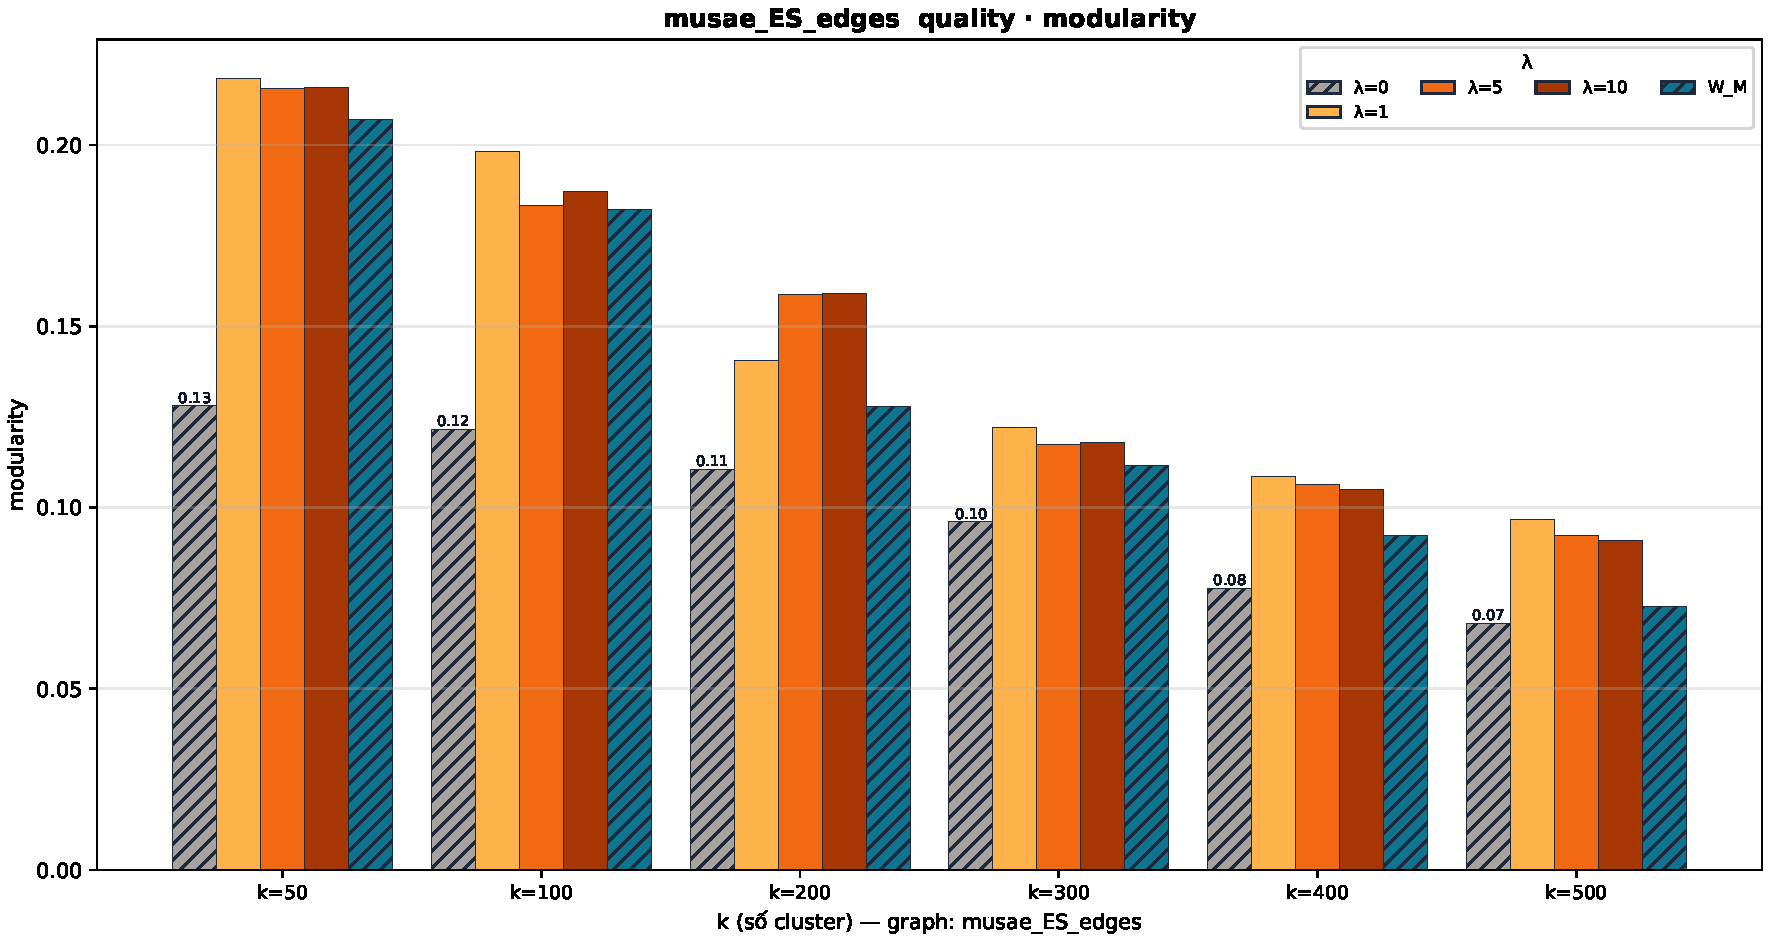
\includegraphics[width=\textwidth]{../main_result/REAL/musae_ES_edges/charts/quality_modularity.pdf}
    \caption{Modularity $Q$ trên musae\_ES theo $\lambda$ và $K$.}
    \label{fig:real-musae-es}
\end{figure}

$Q(0)$ thuộc khoảng $0{,}07$--$0{,}13$, sát chế độ của musae\_DE. Cải thiện lớn nhất tại $K = 50$ với $\Delta Q = +0{,}0902$, tương ứng tăng khoảng $70\%$. $\lambda^* = 1$ ở $K = 50$, nhỏ hơn $W_M$ của musae\_DE, cho thấy đóng góp tối ưu của motif đã đạt ở mức trọng số trung bình.

\textbf{Hệ số phân cụm.}
\begin{figure}[H]
    \centering
    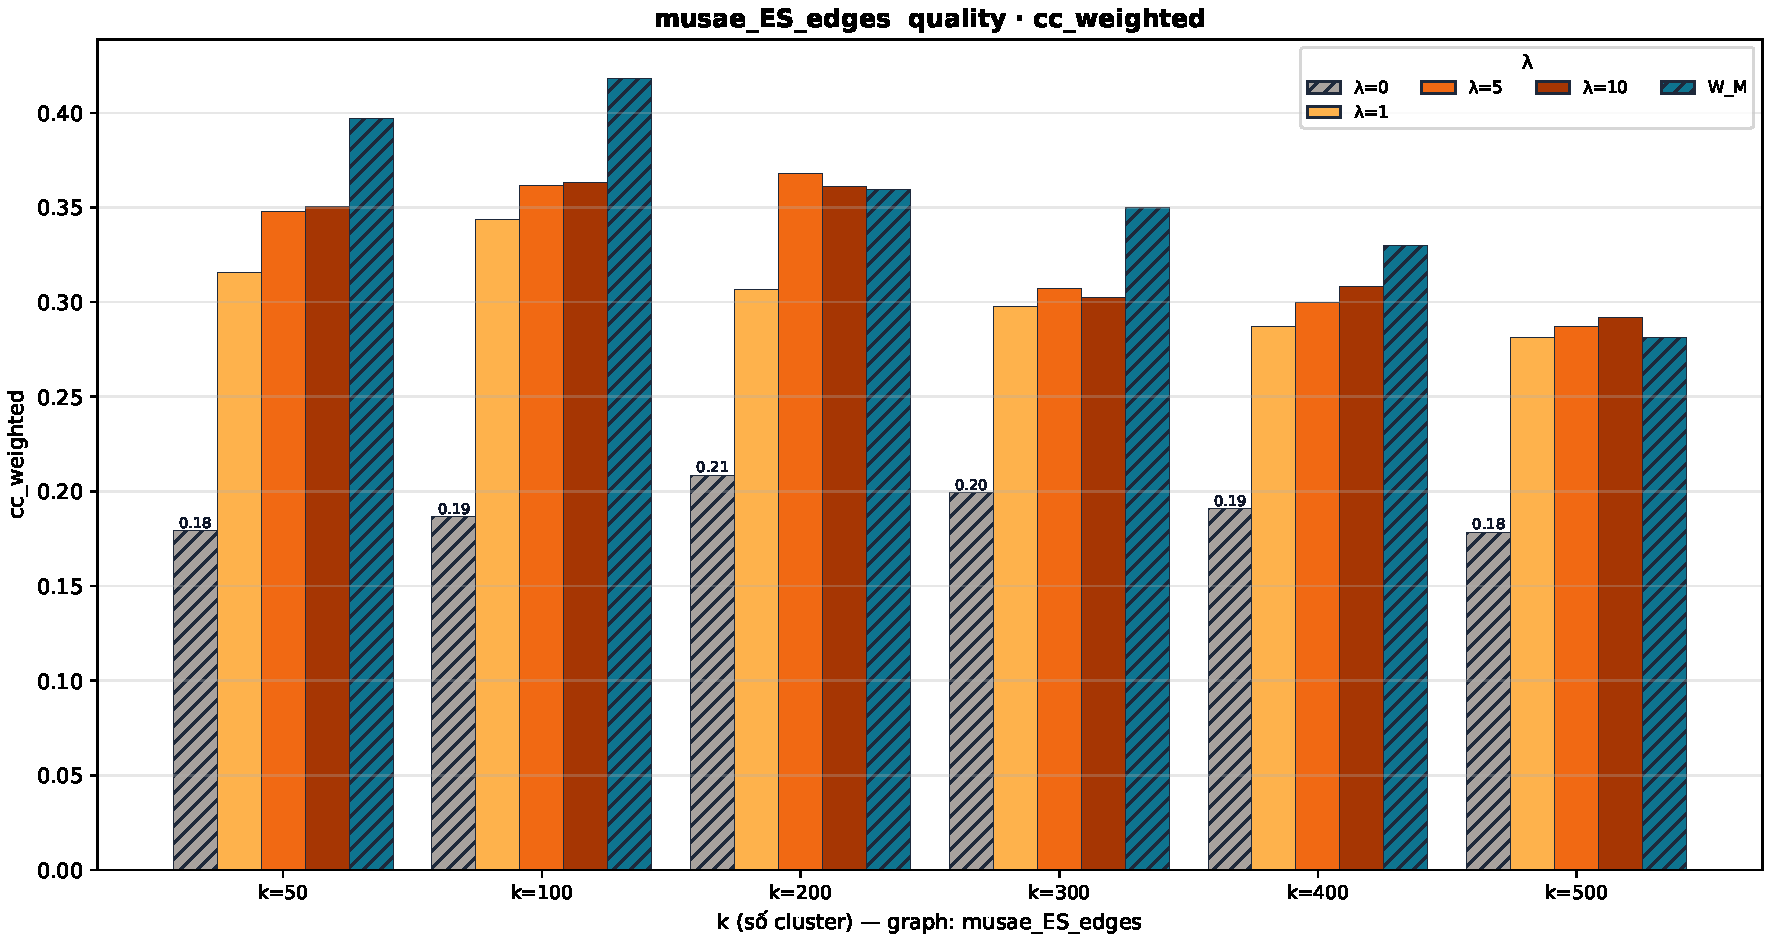
\includegraphics[width=\textwidth]{../main_result/REAL/musae_ES_edges/charts/quality_cc_weighted.pdf}
    \caption{$\overline{\mathrm{CC}}_w$ trên musae\_ES theo $\lambda$ và $K$.}
    \label{fig:real-cc-musae-es}
\end{figure}

\begin{figure}[H]
    \centering
    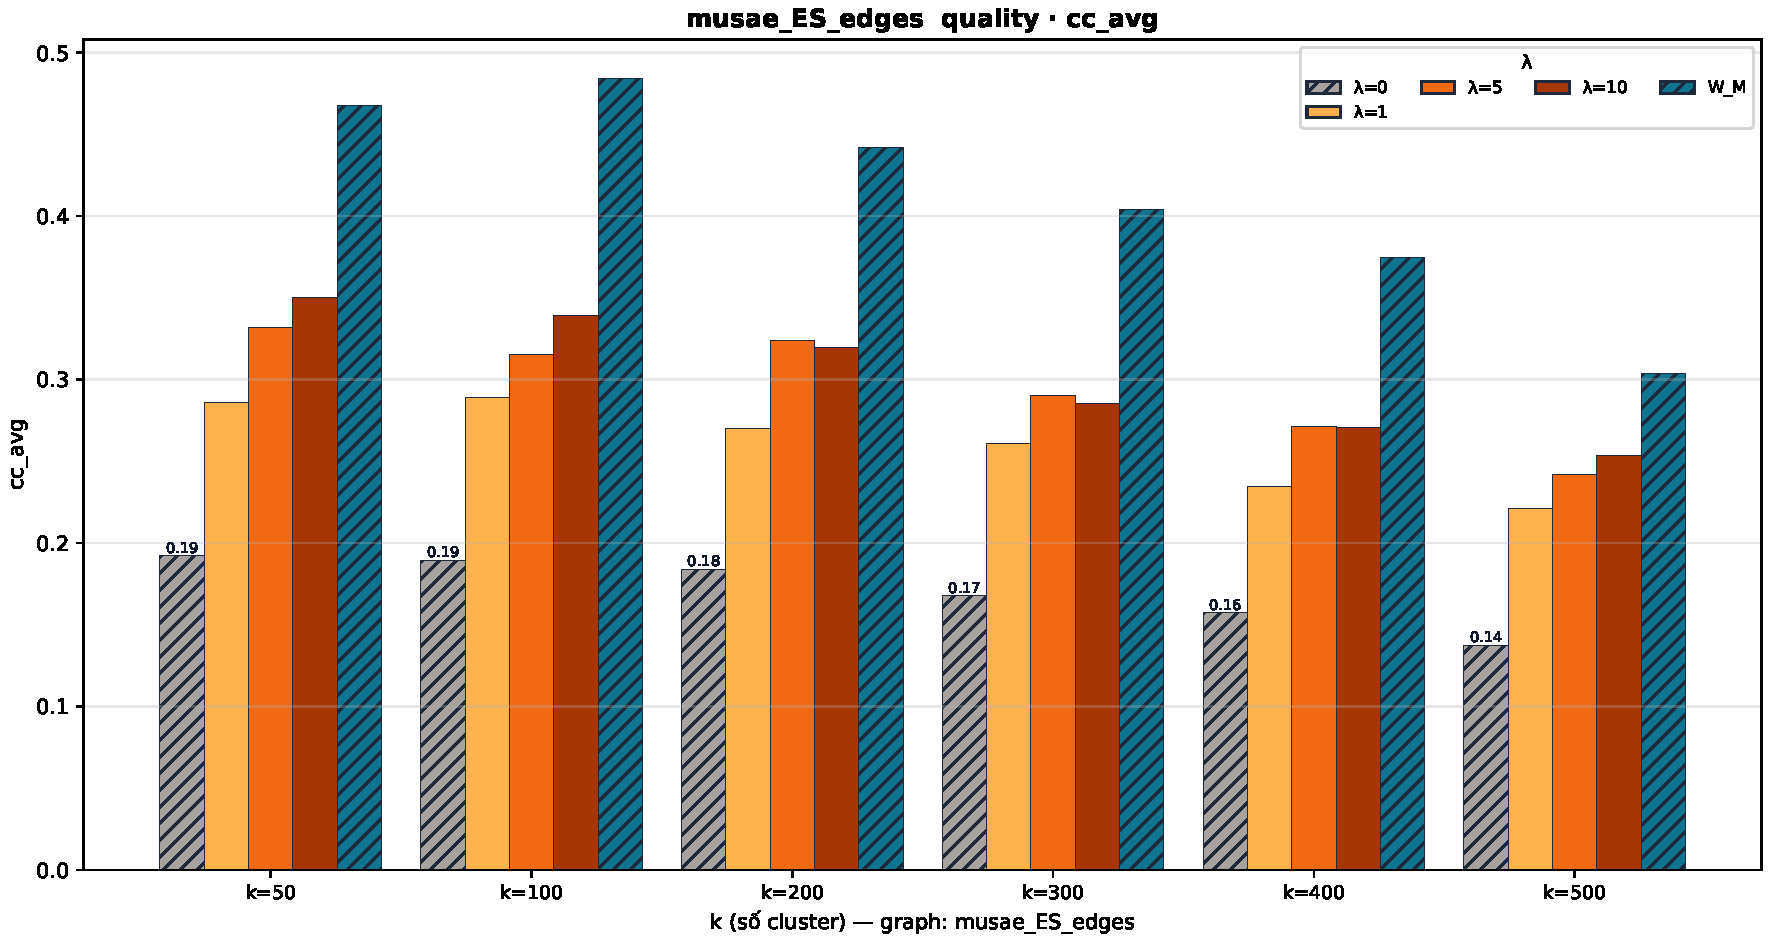
\includegraphics[width=\textwidth]{../main_result/REAL/musae_ES_edges/charts/quality_cc_avg.pdf}
    \caption{$\overline{\mathrm{CC}}$ trên musae\_ES theo $\lambda$ và $K$.}
    \label{fig:real-ccavg-musae-es}
\end{figure}

Tại $K = 50$, $\overline{\mathrm{CC}}_w(0) = 0{,}1793$ vẫn dưới $cc_{\mathrm{global}}$, sau đó tăng lên $0{,}3968$ tại $W_M$, gấp khoảng hai lần. $\overline{\mathrm{CC}}$ bật từ $0{,}3504$ tại $\lambda = 10$ lên $0{,}4678$ tại $W_M$ (tăng $0{,}12$), nhanh hơn rõ rệt so với $\overline{\mathrm{CC}}_w$ (tăng $0{,}05$ trong cùng đoạn). Lặp lại pattern của musae\_DE: $W_M$ tạo nhiều cụm nhỏ thiên lệch $\overline{\mathrm{CC}}$.

\textbf{Kết luận.} Cùng họ với musae\_DE nhưng quy mô nhỏ hơn, musae\_ES tái lập cùng pattern: phân cụm phổ thuần bỏ sót cấu trúc tam giác, trọng số motif khôi phục được tín hiệu cộng đồng. Việc $\lambda^*$ nhỏ hơn (giá trị $1$ thay vì $W_M$) phản ánh quy mô nhỏ làm tín hiệu cạnh đã có đóng góp tương đối, nên không cần trọng số motif cực đại.

% ............................................................
\subsection*{lastfm\_asia}

Đỉnh là một người dùng LastFM ở châu Á, cạnh là quan hệ bạn bè trong nền tảng. Cộng đồng có xu hướng theo quốc gia hoặc sở thích âm nhạc. Hệ số phân cụm toàn cục $cc_{\mathrm{global}} = 0{,}2194$, đồ thị thưa hơn musae.

\textbf{Modularity.}
\begin{figure}[H]
    \centering
    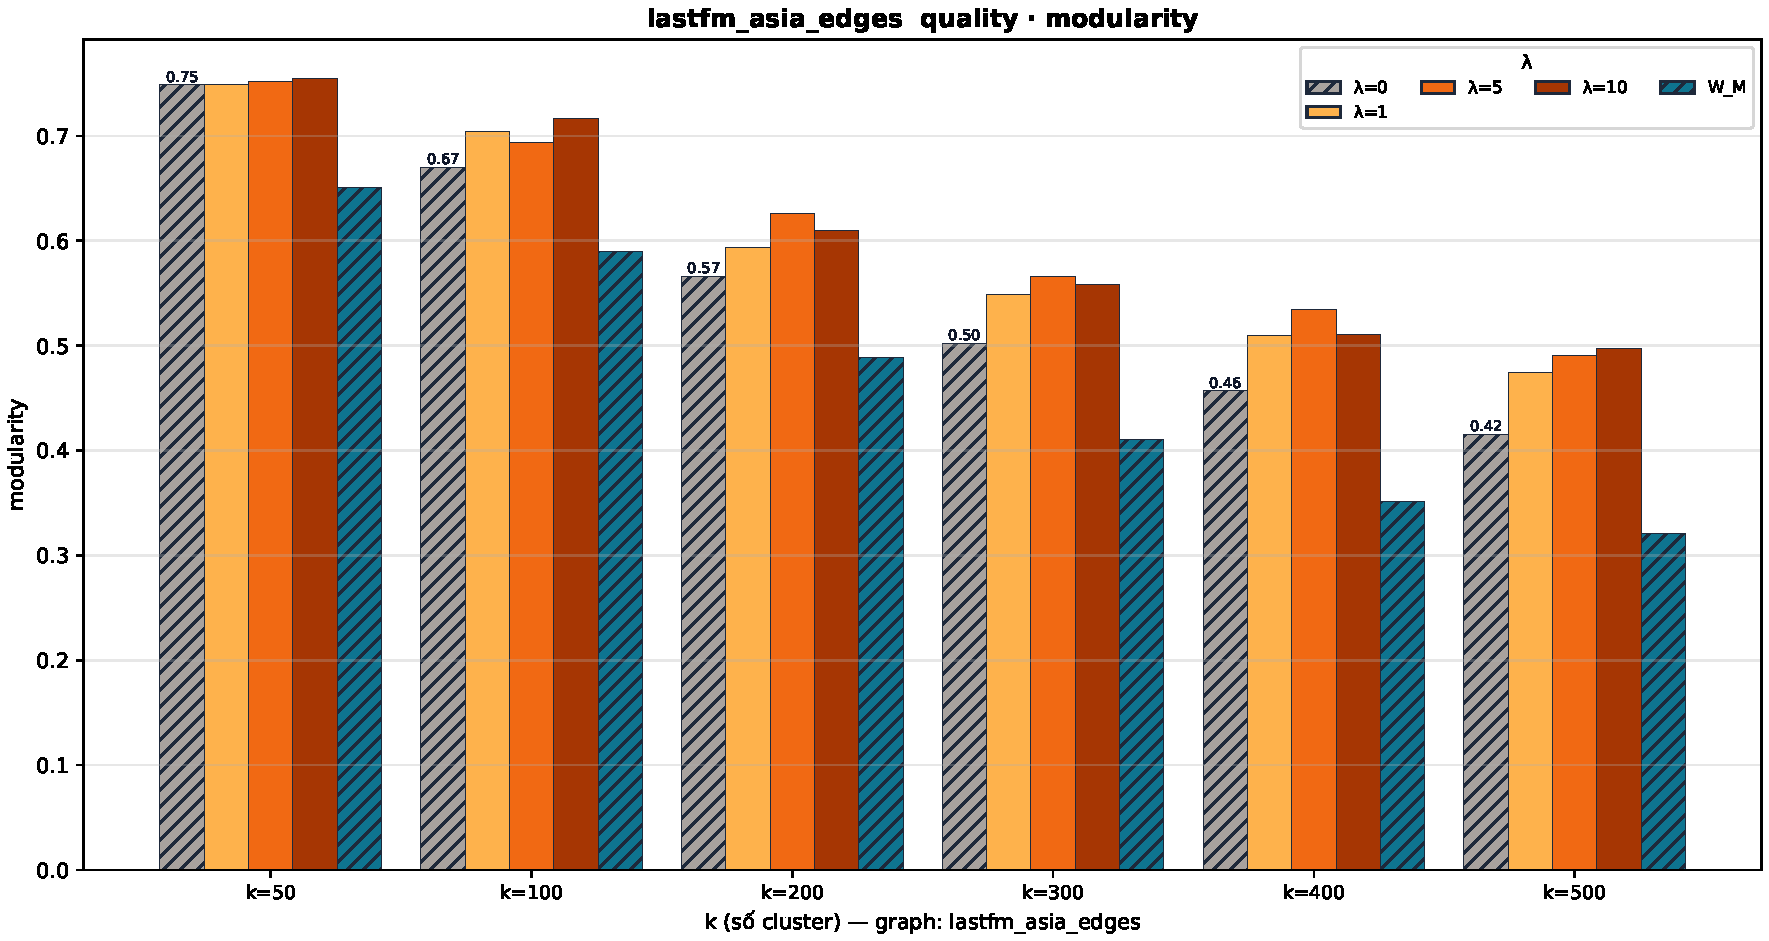
\includegraphics[width=\textwidth]{../main_result/REAL/lastfm_asia_edges/charts/quality_modularity.pdf}
    \caption{Modularity $Q$ trên lastfm\_asia theo $\lambda$ và $K$.}
    \label{fig:real-lastfm}
\end{figure}

Đồ thị này phơi bày cả hai chế độ trên cùng một dataset. Tại $K = 50$, $Q(0) = 0{,}7486$ đã cao và $\Delta Q$ chỉ $+0{,}0059$. Tại $K = 500$, $Q(0)$ tụt còn $0{,}4155$ và $\Delta Q$ vọt lên $+0{,}0815$ với $\lambda^* = 10$. Mức độ cải thiện do trọng số motif tỉ lệ nghịch với chất lượng phân hoạch ban đầu.

\textbf{Hệ số phân cụm.}
\begin{figure}[H]
    \centering
    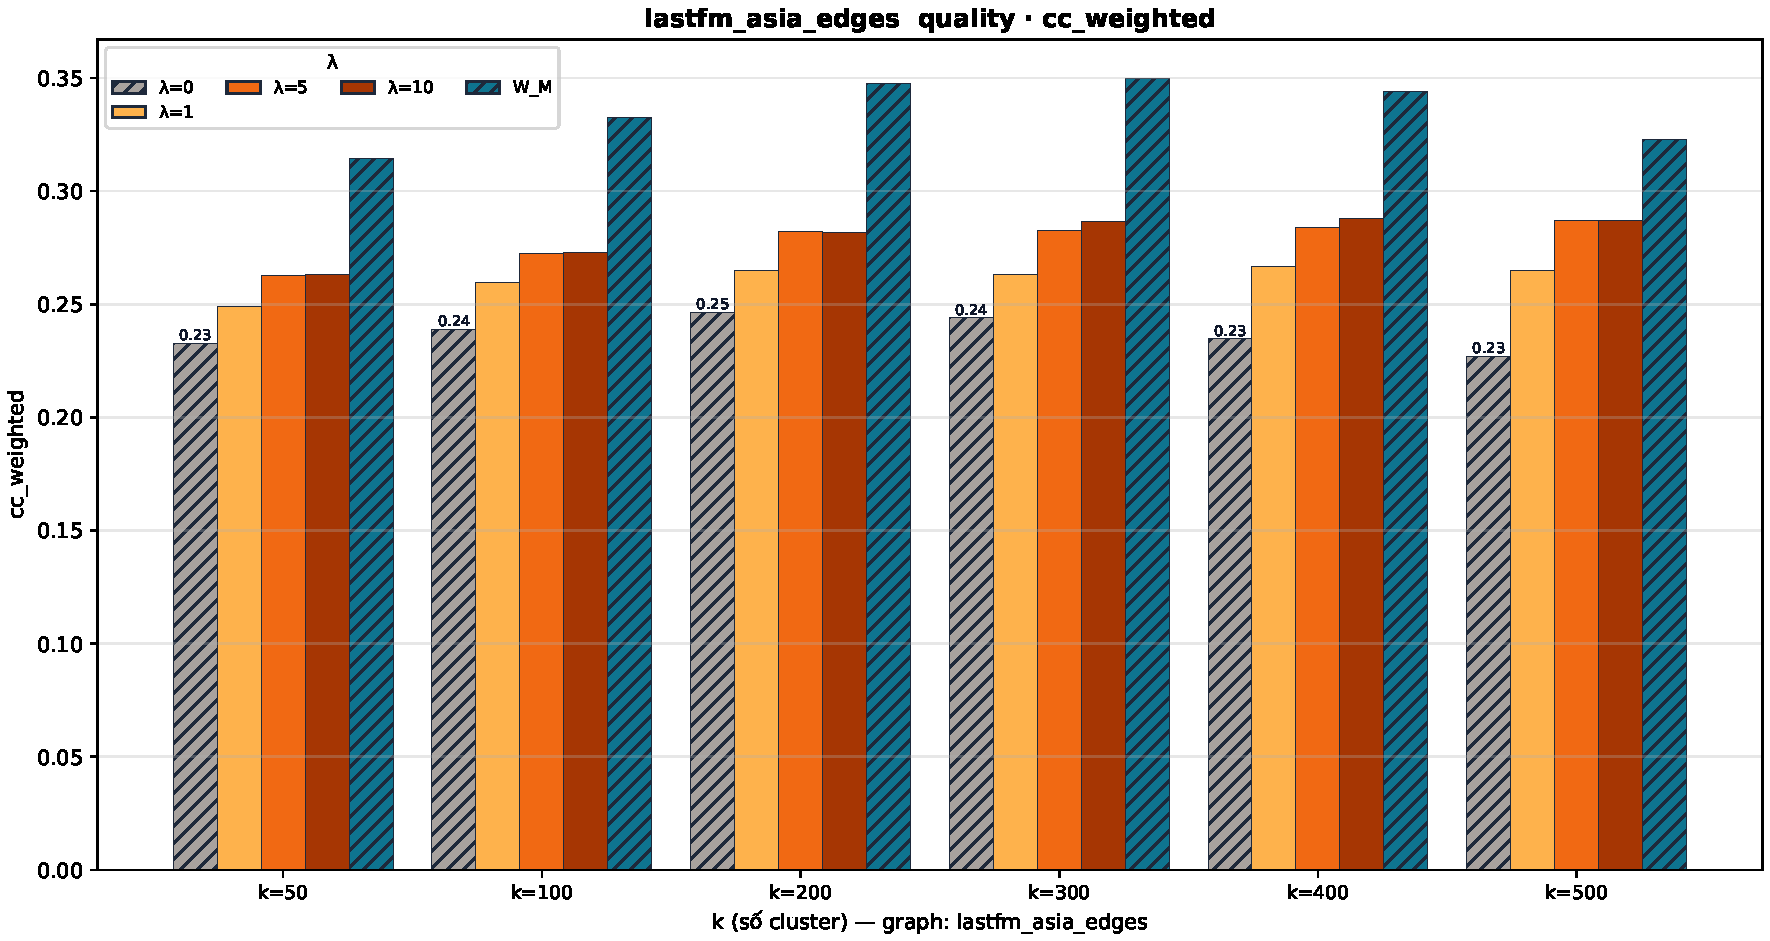
\includegraphics[width=\textwidth]{../main_result/REAL/lastfm_asia_edges/charts/quality_cc_weighted.pdf}
    \caption{$\overline{\mathrm{CC}}_w$ trên lastfm\_asia theo $\lambda$ và $K$.}
    \label{fig:real-cc-lastfm}
\end{figure}

\begin{figure}[H]
    \centering
    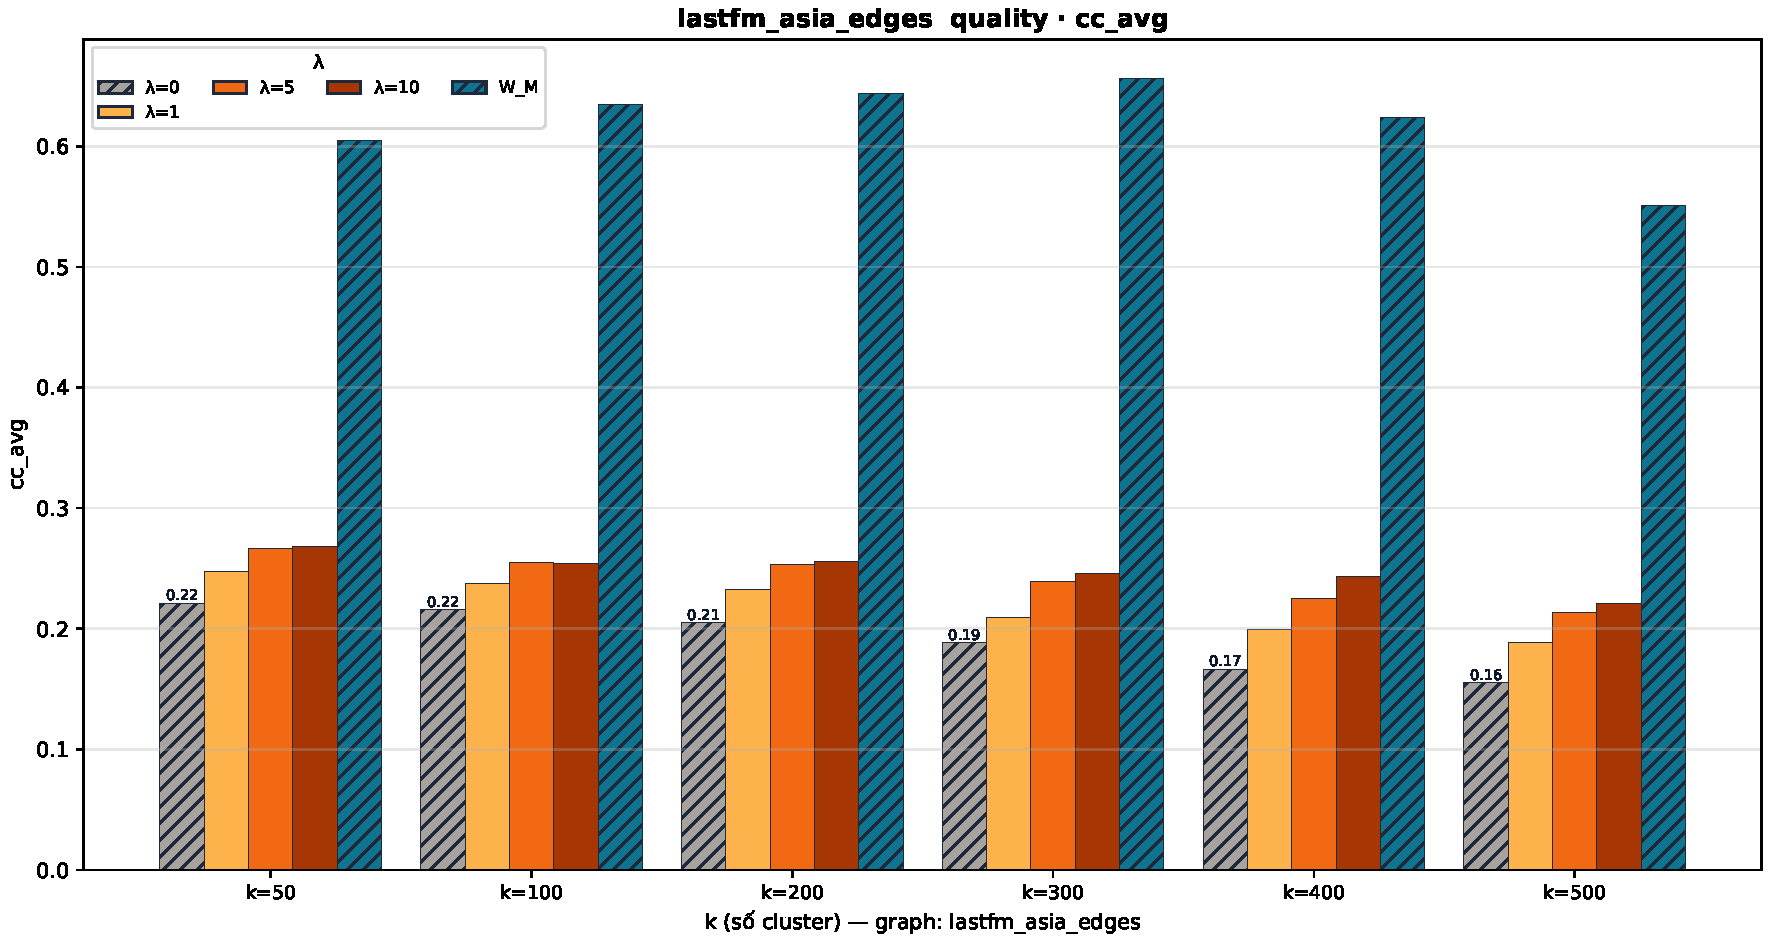
\includegraphics[width=\textwidth]{../main_result/REAL/lastfm_asia_edges/charts/quality_cc_avg.pdf}
    \caption{$\overline{\mathrm{CC}}$ trên lastfm\_asia theo $\lambda$ và $K$.}
    \label{fig:real-ccavg-lastfm}
\end{figure}

Tại $K = 50$, $\overline{\mathrm{CC}}_w(0) = 0{,}2328$ đã gần $cc_{\mathrm{global}}$, tăng lên $0{,}3146$ tại $W_M$. $\overline{\mathrm{CC}}$ tại $W_M$ đạt $0{,}6044$, chênh tới $0{,}29$ so với $\overline{\mathrm{CC}}_w$, lớn nhất trong toàn bộ tập dữ liệu thật; con số này bật từ $0{,}2681$ tại $\lambda = 10$ chỉ qua một bước. Đây là minh hoạ rõ nhất cho hiện tượng phân mảnh cụm khi $\lambda \to \infty$ đã trình bày ở Định nghĩa~\ref{def:cc-cluster}: $W_M$ sinh nhiều cụm rất nhỏ với hệ số phân cụm cục bộ cao, đẩy $\overline{\mathrm{CC}}$ vọt lên trong khi $\overline{\mathrm{CC}}_w$ tiếp tục cho con số thận trọng.

\textbf{Kết luận.} lastfm\_asia là ví dụ điển hình về đồ thị xã hội thưa với cộng đồng đa quy mô. Tại $K$ nhỏ, các cụm lớn đã định hình tốt qua cạnh; tại $K$ lớn, cần bóc tách thêm các nhóm sở thích nhỏ và motif đóng vai trò quan trọng. Chênh lệch lớn giữa $\overline{\mathrm{CC}}$ và $\overline{\mathrm{CC}}_w$ khẳng định lựa chọn $\overline{\mathrm{CC}}_w$ làm chỉ số chính: nếu dùng $\overline{\mathrm{CC}}$, chất lượng phân hoạch trên đồ thị này sẽ bị đánh giá quá lạc quan.

% ............................................................
\subsection*{Email-Enron}

Đỉnh là một địa chỉ email nội bộ công ty Enron, cạnh nếu có ít nhất một thư trao đổi giữa hai địa chỉ. Cộng đồng có nghĩa là phòng ban hoặc nhóm dự án. Hệ số phân cụm toàn cục $cc_{\mathrm{global}} = 0{,}5092$ ở mức cao, phản ánh trao đổi email ba bên trong cùng phòng ban.

\textbf{Modularity.}
\begin{figure}[H]
    \centering
    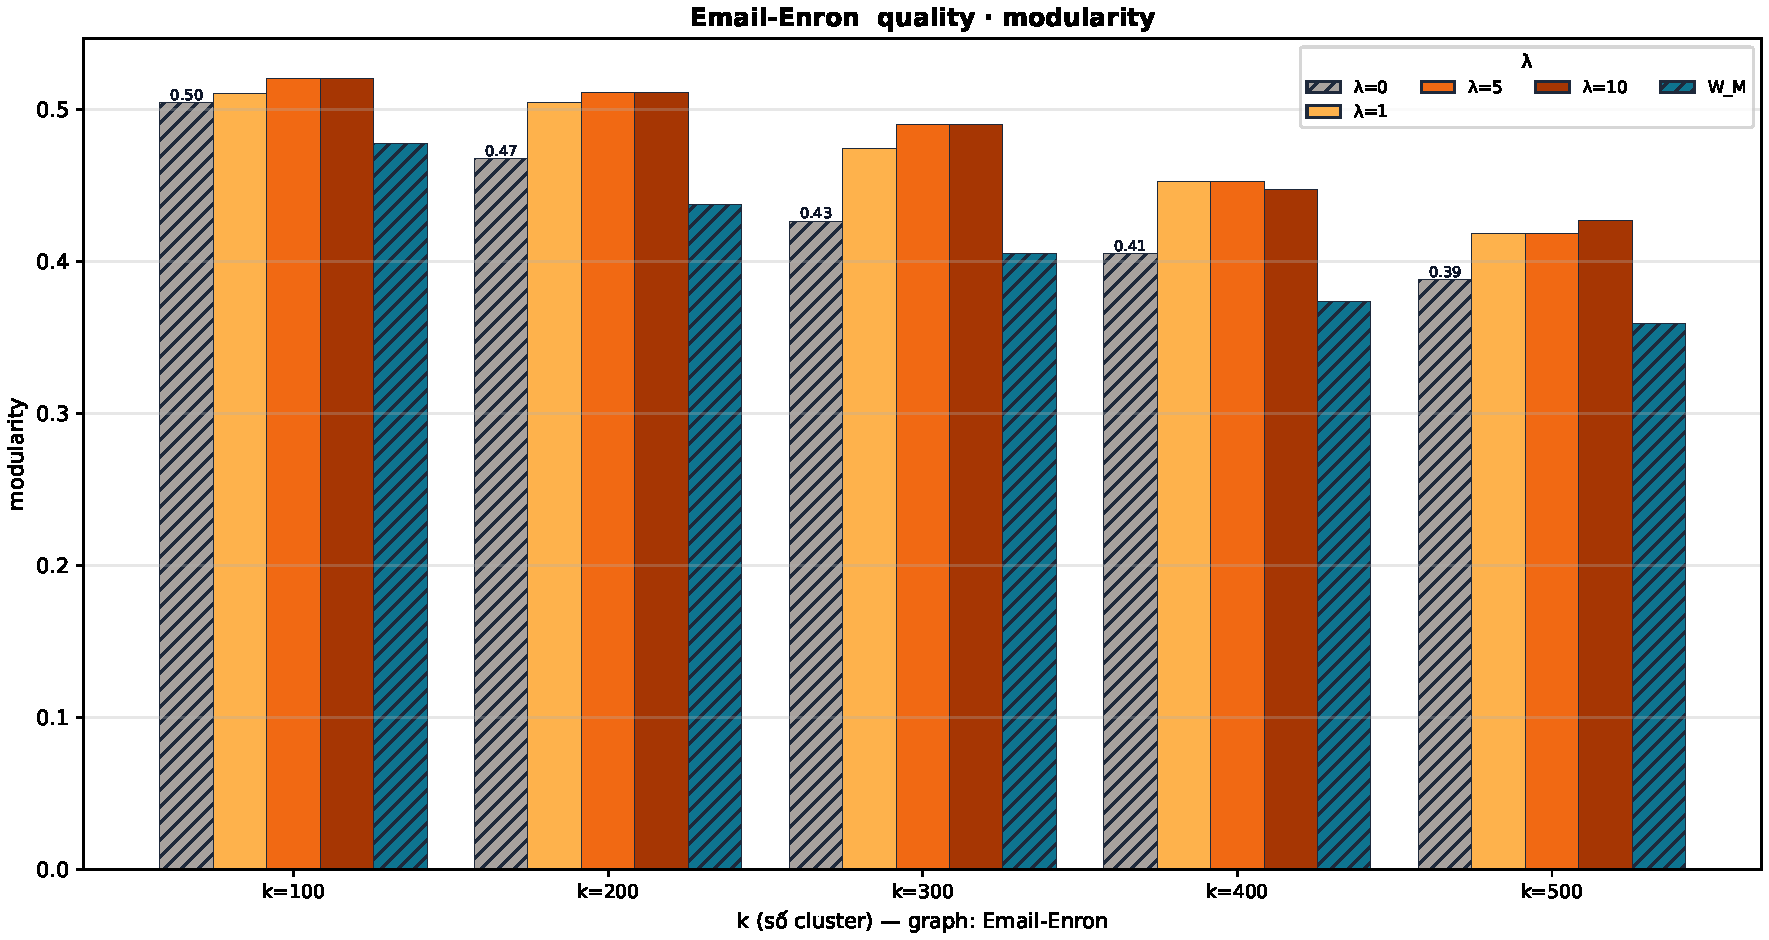
\includegraphics[width=\textwidth]{../main_result/REAL/Email-Enron/charts/quality_modularity.pdf}
    \caption{Modularity $Q$ trên Email-Enron theo $\lambda$ và $K$.}
    \label{fig:real-enron}
\end{figure}

$Q(0)$ thuộc vùng trung gian ($0{,}39$--$0{,}50$). Cải thiện đáng kể trên mọi $K$, $\Delta Q$ dao động từ $+0{,}016$ tại $K = 100$ đến $+0{,}064$ tại $K = 300$, bám sát quy luật $Q(0)$ càng thấp thì $\Delta Q$ càng lớn. Tại $K = 300$, $\lambda^* = 5$.

\textbf{Hệ số phân cụm.}
\begin{figure}[H]
    \centering
    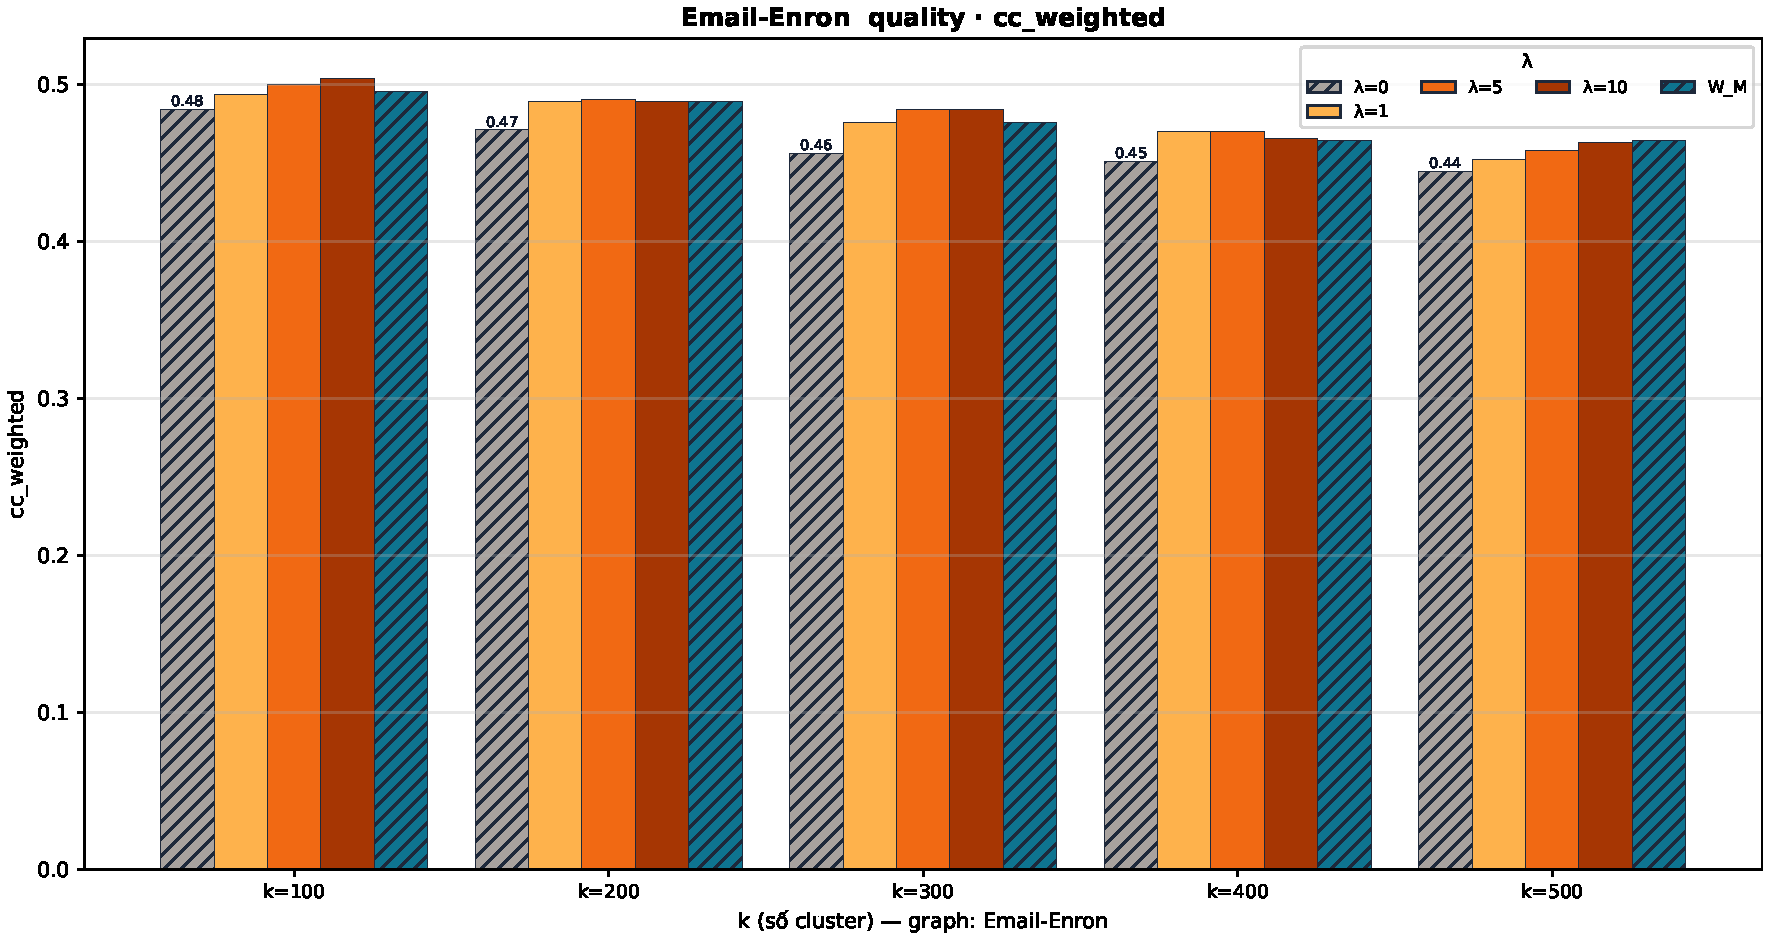
\includegraphics[width=\textwidth]{../main_result/REAL/Email-Enron/charts/quality_cc_weighted.pdf}
    \caption{$\overline{\mathrm{CC}}_w$ trên Email-Enron theo $\lambda$ và $K$.}
    \label{fig:real-cc-enron}
\end{figure}

\begin{figure}[H]
    \centering
    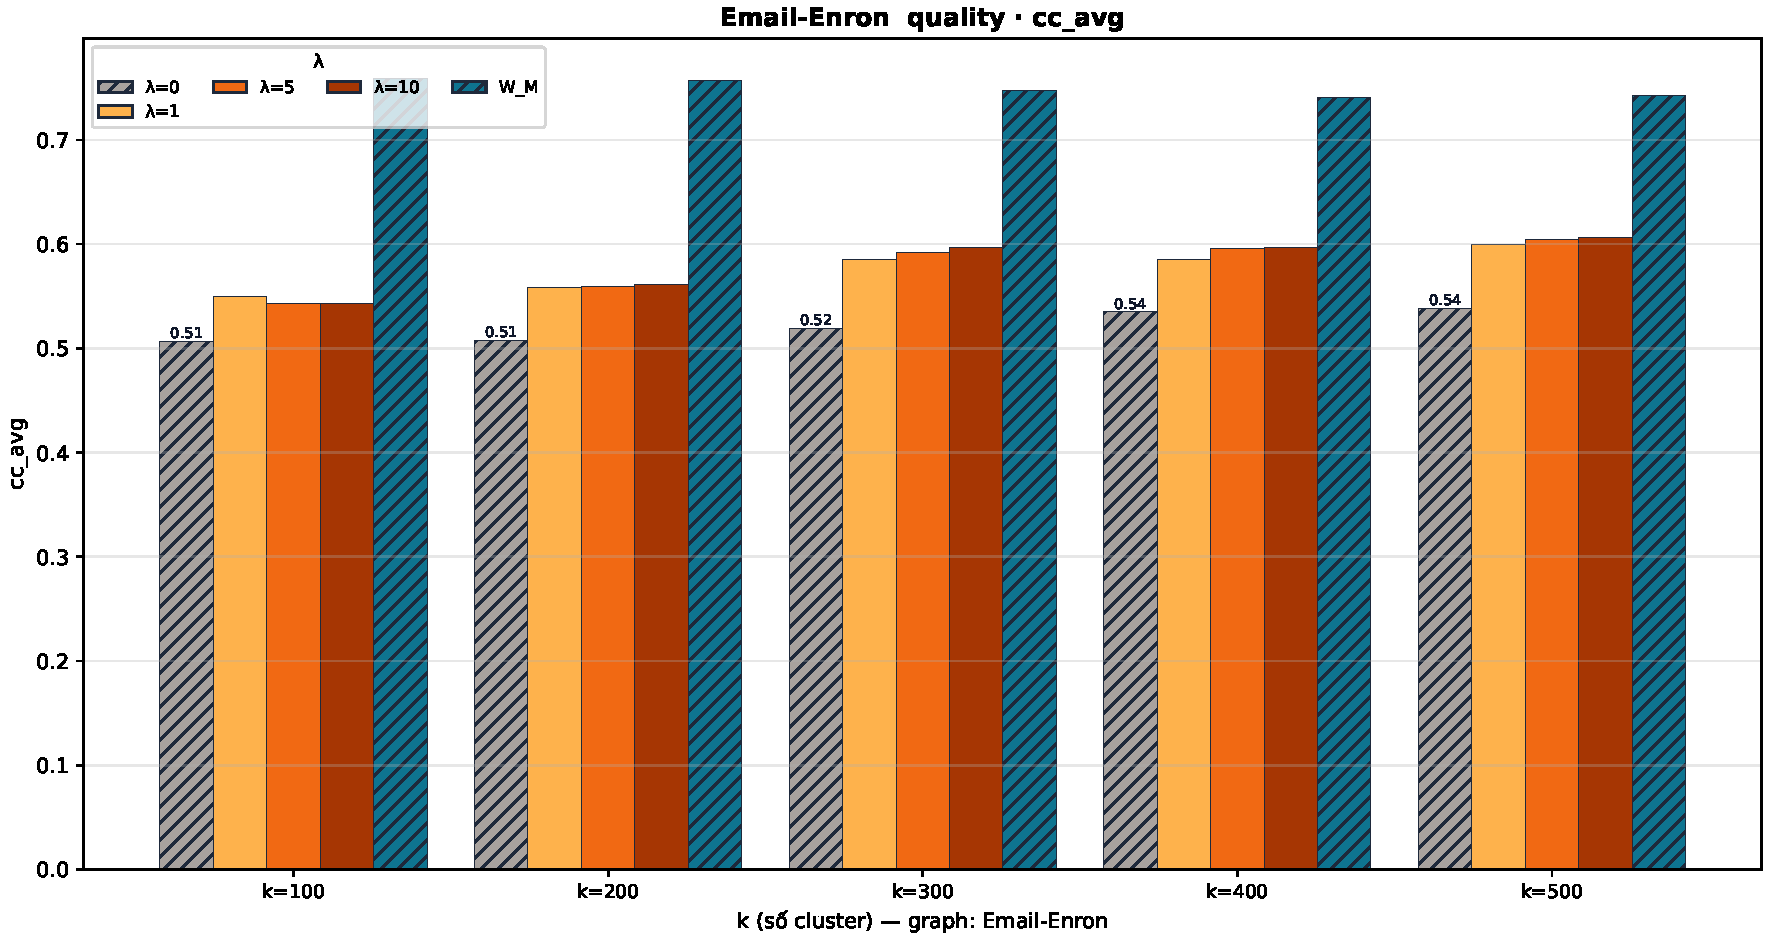
\includegraphics[width=\textwidth]{../main_result/REAL/Email-Enron/charts/quality_cc_avg.pdf}
    \caption{$\overline{\mathrm{CC}}$ trên Email-Enron theo $\lambda$ và $K$.}
    \label{fig:real-ccavg-enron}
\end{figure}

Tại $K = 100$, $\overline{\mathrm{CC}}_w(0) = 0{,}4844$ đã sát $cc_{\mathrm{global}}$. Mức tăng nhẹ lên $0{,}5040$ tại $\lambda = 10$ là biên độ điển hình của đồ thị có $cc_{\mathrm{global}}$ cao. $\overline{\mathrm{CC}}$ tại $\lambda = 10$ chênh $0{,}04$ so với $\overline{\mathrm{CC}}_w$ ($0{,}5432$ so với $0{,}5040$), nhưng tại $W_M$ bật lên $0{,}7592$ trong khi $\overline{\mathrm{CC}}_w$ tụt còn $0{,}4959$, mở rộng chênh lệch lên $0{,}26$. Đây là một trong những trường hợp $W_M$ làm phân mảnh cụm rõ nhất, được $\overline{\mathrm{CC}}_w$ phát hiện và phạt đúng.

\textbf{Kết luận.} Email-Enron thuộc nhóm đồ thị có cấu trúc tam giác đã được phân cụm phổ trên $A$ khai thác tốt, khoảng cải thiện CC còn lại cho $W_\lambda$ tương đối hẹp. Tuy nhiên modularity vẫn cải thiện đáng kể, cho thấy motif giúp tinh chỉnh ranh giới cụm chứ không tạo ra cấu trúc tam giác mới.

% ............................................................
\subsection*{facebook\_combined}

Hợp của mười ego-network: với mỗi trong mười người dùng Facebook, ta lấy đồ thị bạn bè của họ rồi ghép lại. Đỉnh là người dùng, cạnh là quan hệ bạn bè. Cộng đồng có nghĩa là vòng quan hệ xã hội của từng ego. Hệ số phân cụm toàn cục $cc_{\mathrm{global}} = 0{,}6055$ rất cao, đặc trưng của cấu trúc ego-network.

\textbf{Modularity.}
\begin{figure}[H]
    \centering
    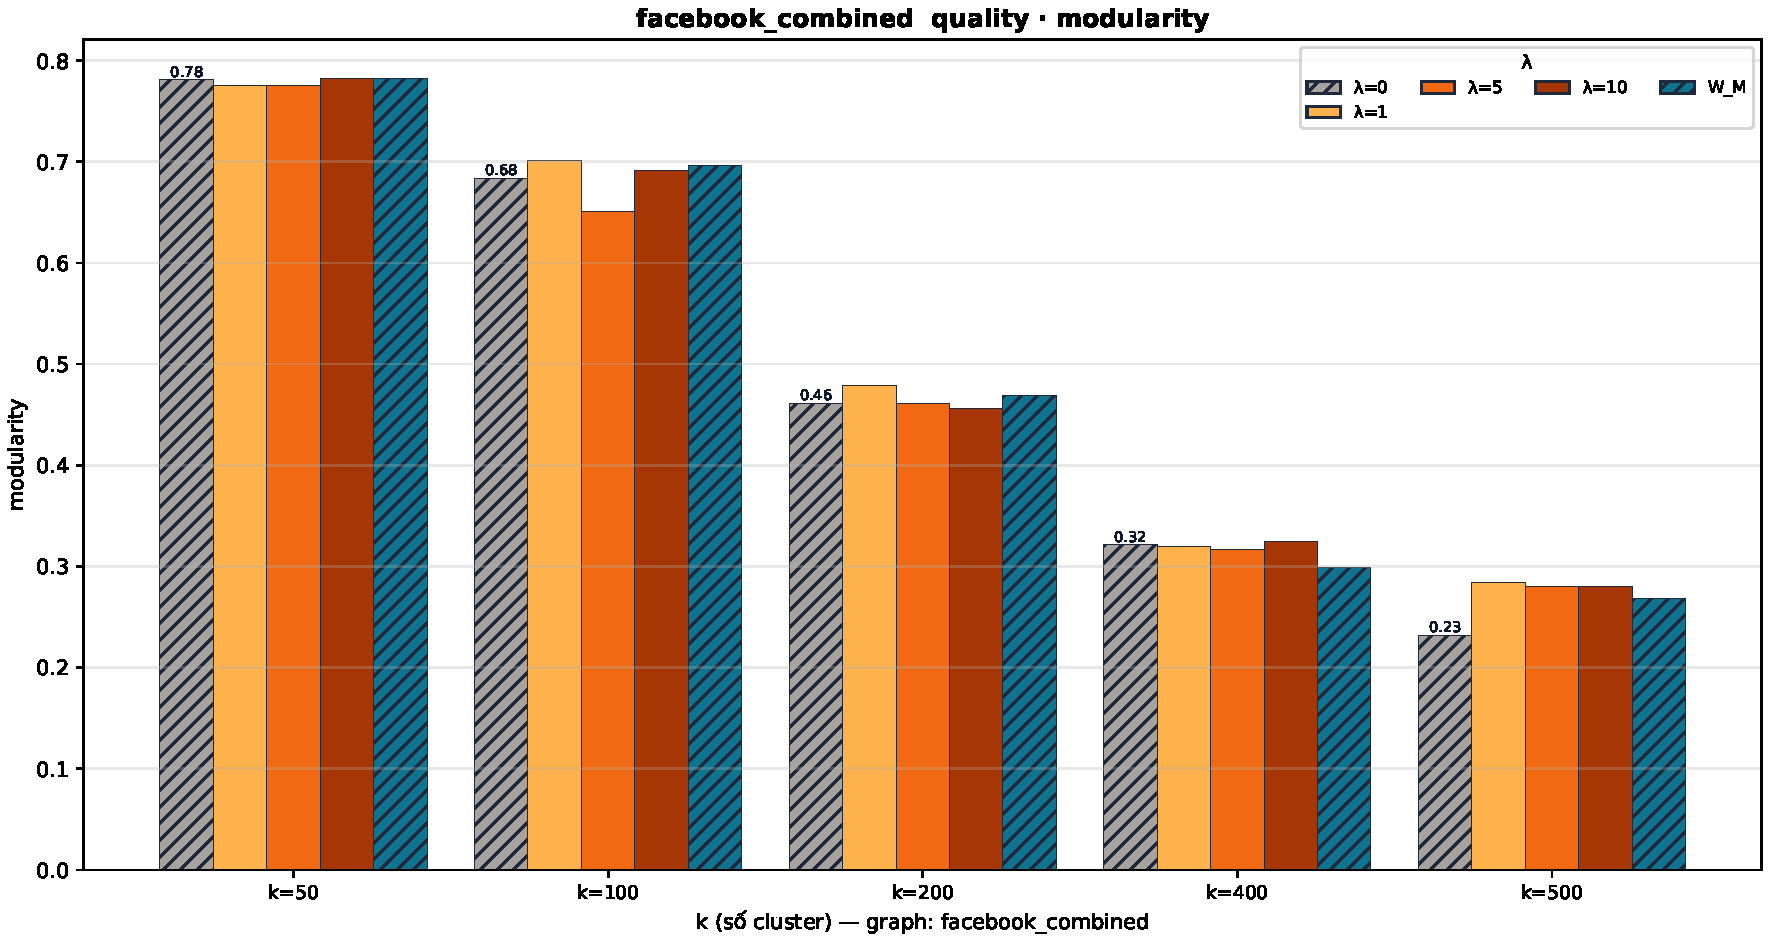
\includegraphics[width=\textwidth]{../main_result/REAL/facebook_combined/charts/quality_modularity.pdf}
    \caption{Modularity $Q$ trên facebook\_combined theo $\lambda$ và $K$.}
    \label{fig:real-facebook}
\end{figure}

Tại $K = 50$, $Q(0) = 0{,}7810$ rất cao và $\Delta Q = +0{,}0010$ không đáng kể. Khi tăng $K$ lên $500$, $Q(0)$ tụt còn $0{,}2319$ và $\Delta Q$ đạt $+0{,}0519$ với $\lambda^* = 5$. Cùng đồ thị nhưng hai chế độ tách biệt theo $K$.

\textbf{Hệ số phân cụm.}
\begin{figure}[H]
    \centering
    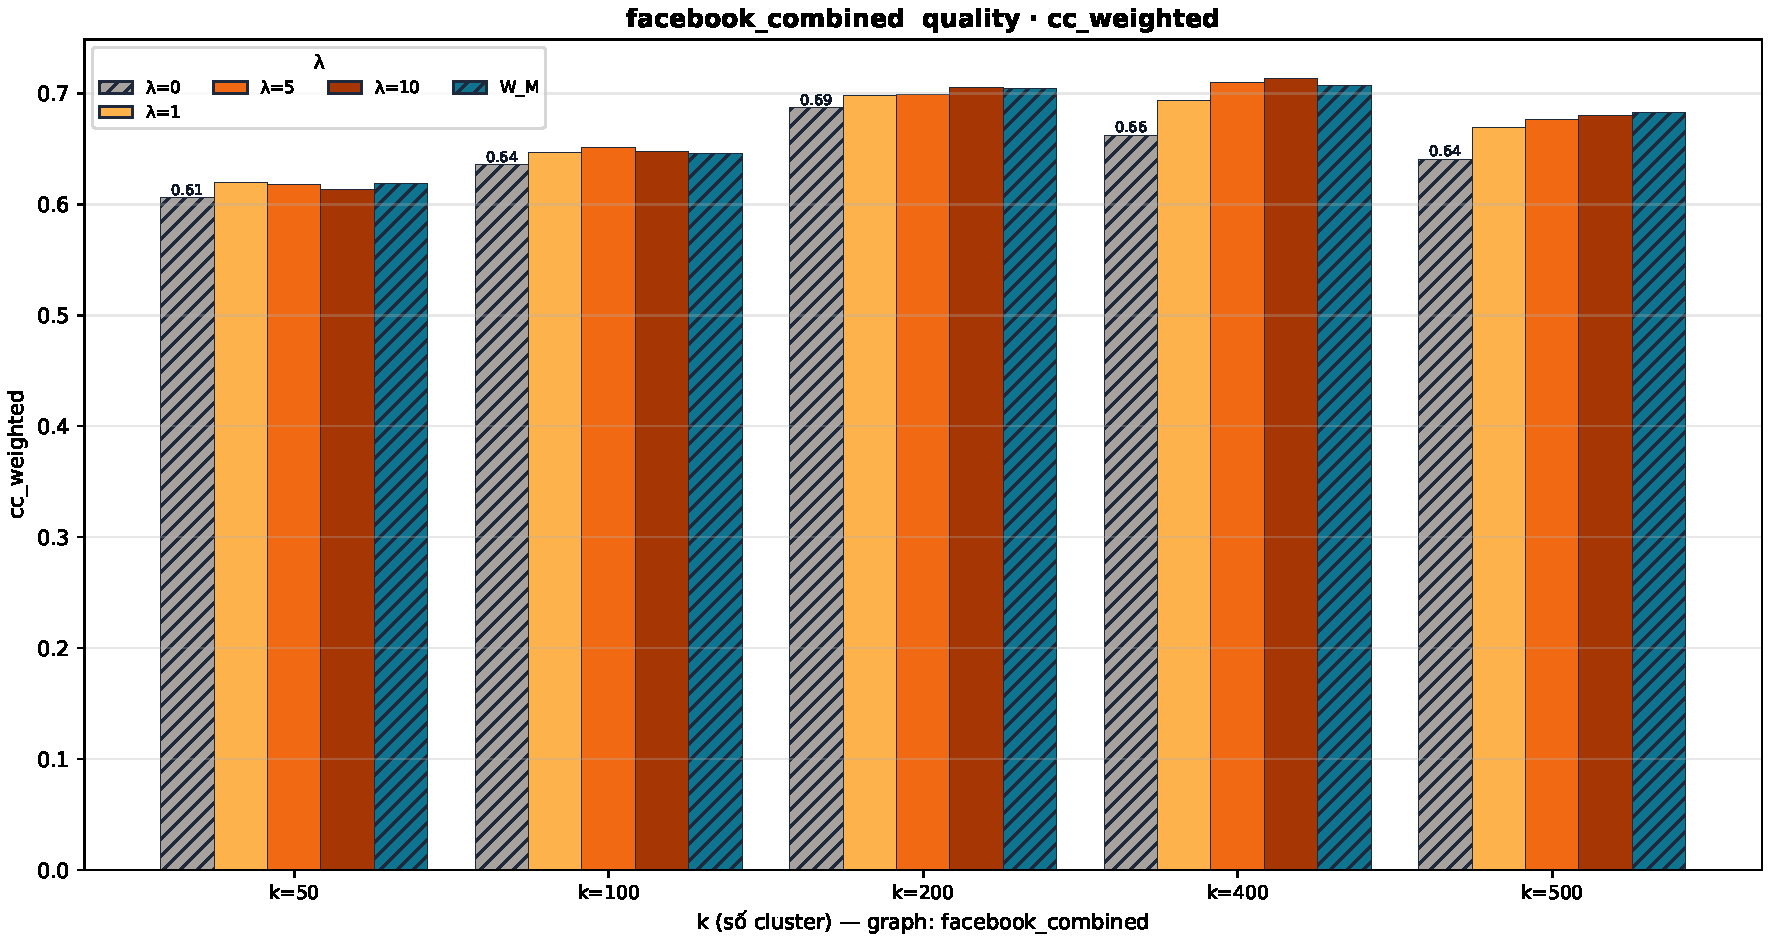
\includegraphics[width=\textwidth]{../main_result/REAL/facebook_combined/charts/quality_cc_weighted.pdf}
    \caption{$\overline{\mathrm{CC}}_w$ trên facebook\_combined theo $\lambda$ và $K$.}
    \label{fig:real-cc-facebook}
\end{figure}

\begin{figure}[H]
    \centering
    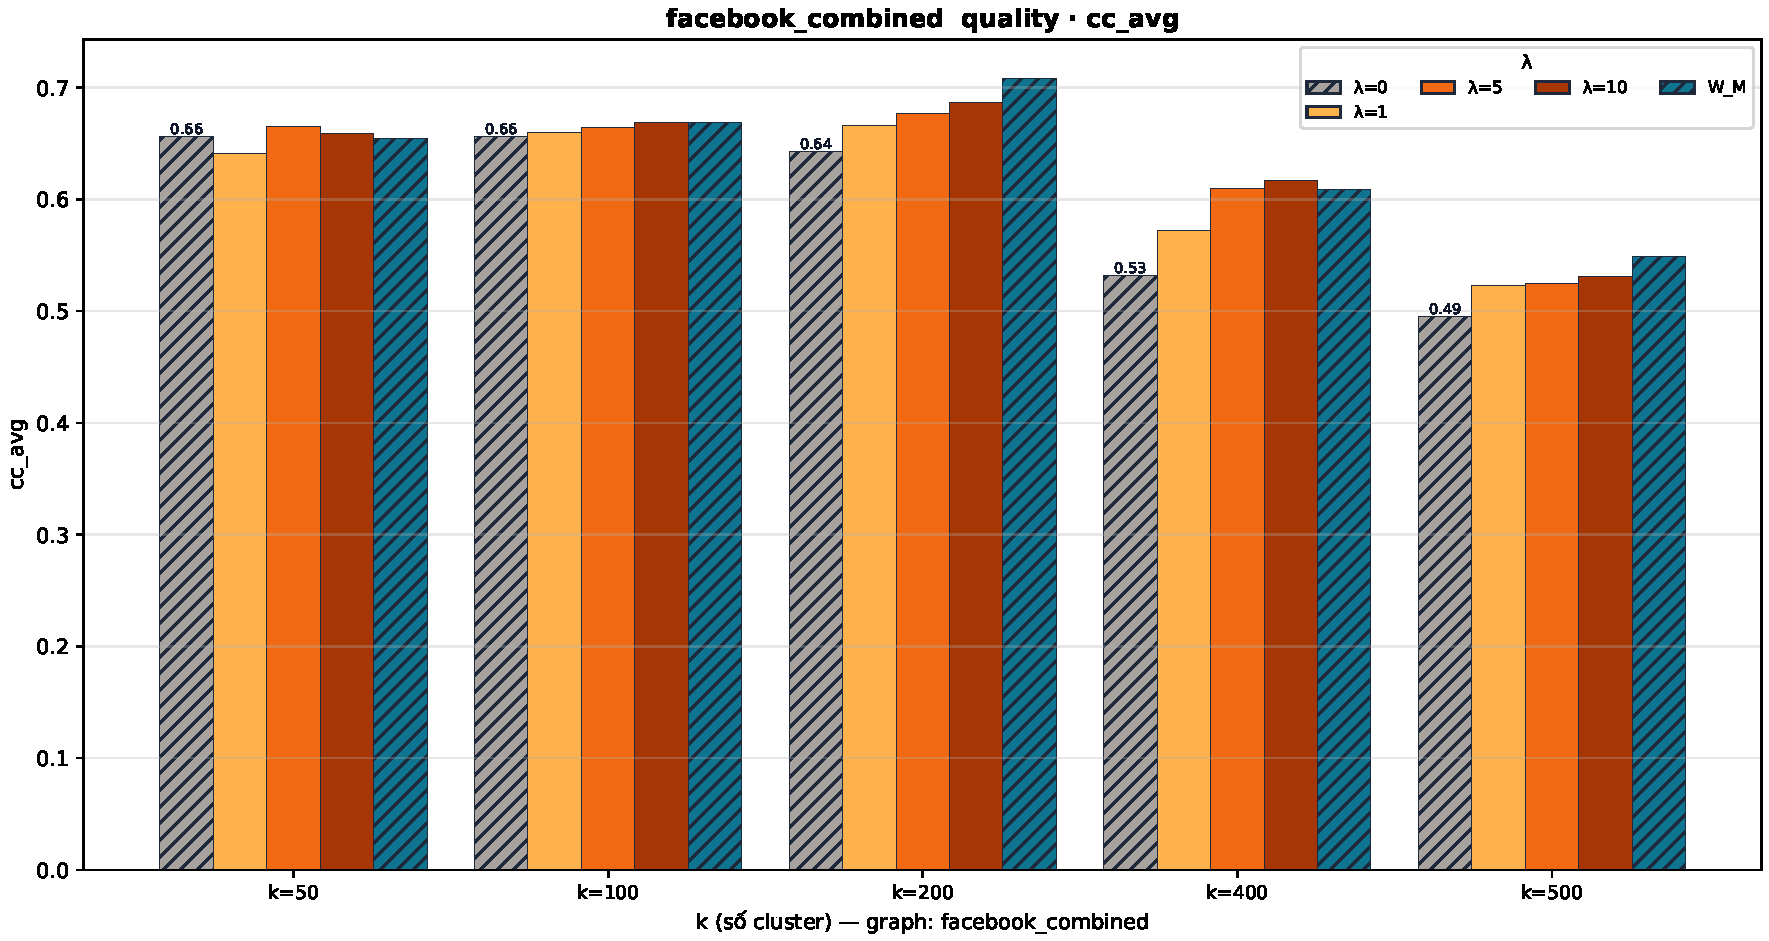
\includegraphics[width=\textwidth]{../main_result/REAL/facebook_combined/charts/quality_cc_avg.pdf}
    \caption{$\overline{\mathrm{CC}}$ trên facebook\_combined theo $\lambda$ và $K$.}
    \label{fig:real-ccavg-facebook}
\end{figure}

Tại $K = 50$, $\overline{\mathrm{CC}}_w(0) = 0{,}6061$ trùng khớp với $cc_{\mathrm{global}}$. Mức tăng theo $\lambda$ rất nhỏ, đạt $0{,}6192$ tại $\lambda = 1$. Khác biệt với phần lớn đồ thị thật, $\overline{\mathrm{CC}}$ tại $W_M$ không bật lên mạnh ($0{,}6548$, gần với giá trị tại $\lambda = 10$ là $0{,}6587$); $\overline{\mathrm{CC}}_w$ cùng giữ ổn định. Cấu trúc ego-network bền vững khiến phân hoạch không bị phân mảnh ngay cả khi bỏ ma trận kề.

\textbf{Kết luận.} facebook\_combined là đồ thị ego-network với cấu trúc tam giác đã trùng khớp gần như hoàn hảo với cộng đồng vòng bạn bè. Khi $K$ nhỏ, mỗi ego tạo thành một cụm tự nhiên và phân cụm phổ trên $A$ đã đạt gần tối đa; vai trò của $W_\lambda$ chỉ rõ rệt khi tăng $K$ để chia tiếp các vòng bạn bè con bên trong mỗi ego.

% ............................................................
\subsection*{CA-GrQc}

Mạng đồng tác giả trên arXiv lĩnh vực Tương đối tổng quát. Đỉnh là một tác giả, cạnh nếu hai tác giả cùng đứng tên trên ít nhất một bài báo. Cộng đồng có nghĩa là nhóm nghiên cứu thường xuyên hợp tác. Hệ số phân cụm toàn cục $cc_{\mathrm{global}} = 0{,}5569$, do bài báo nhiều tác giả tự nhiên sinh tam giác đầy đủ giữa đồng tác giả.

\textbf{Modularity.}
\begin{figure}[H]
    \centering
    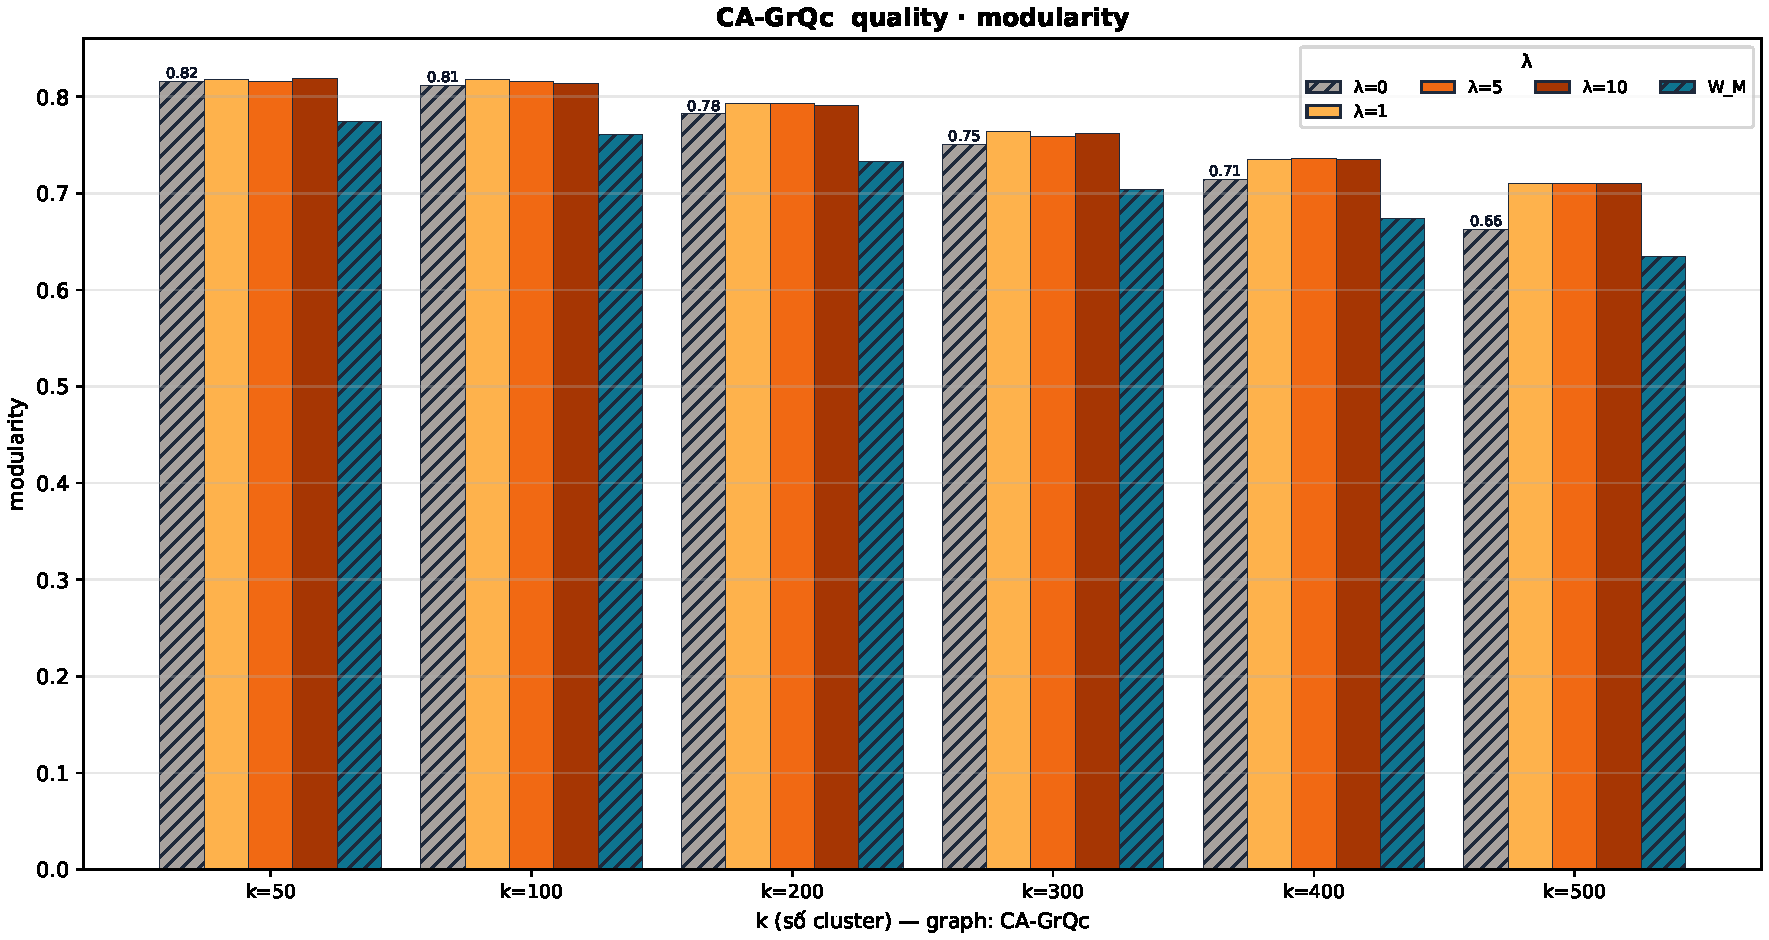
\includegraphics[width=\textwidth]{../main_result/REAL/CA-GrQc/charts/quality_modularity.pdf}
    \caption{Modularity $Q$ trên CA-GrQc theo $\lambda$ và $K$.}
    \label{fig:real-grqc}
\end{figure}

$Q(0)$ cao trên dải rộng ($0{,}66$--$0{,}82$). Tại $K = 50$, $Q(0) = 0{,}8161$ và $\Delta Q = +0{,}0031$ không đáng kể. Chỉ ở $K = 500$ với $Q(0) = 0{,}6630$ thấp hơn, $\Delta Q$ mới đạt $+0{,}0476$ với $\lambda^* = 5$. Phân hoạch chất lượng cao gần như không hưởng lợi từ ma trận hỗn hợp.

\textbf{Hệ số phân cụm.}
\begin{figure}[H]
    \centering
    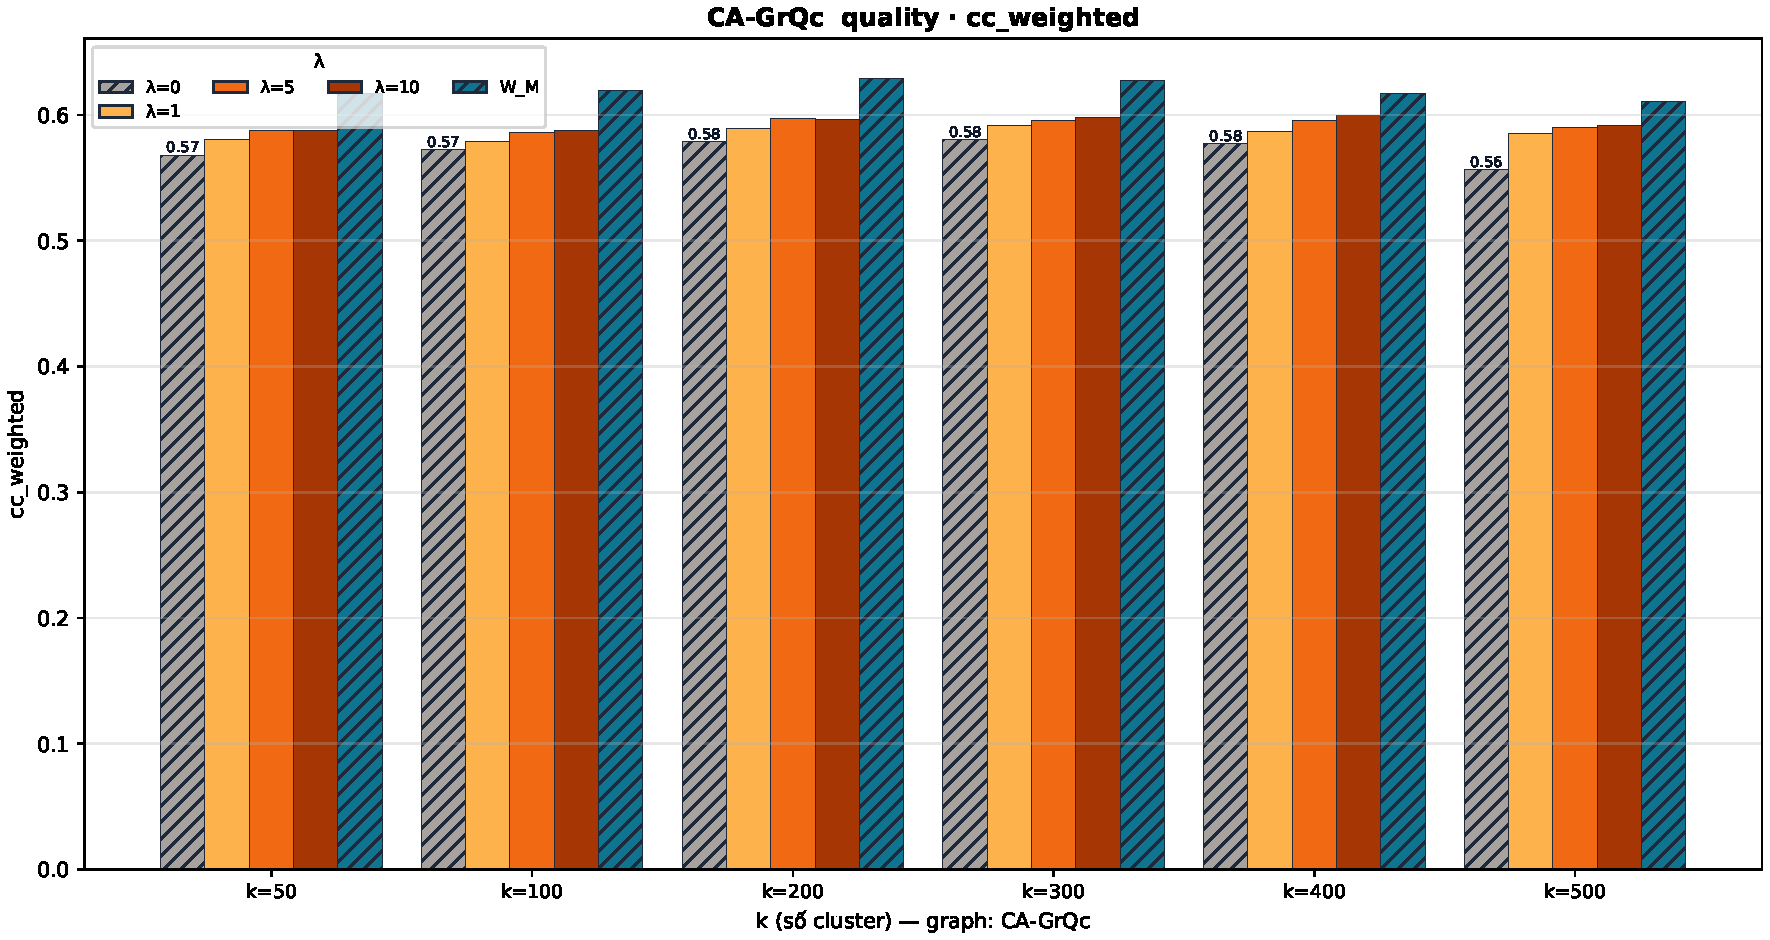
\includegraphics[width=\textwidth]{../main_result/REAL/CA-GrQc/charts/quality_cc_weighted.pdf}
    \caption{$\overline{\mathrm{CC}}_w$ trên CA-GrQc theo $\lambda$ và $K$.}
    \label{fig:real-cc-grqc}
\end{figure}

\begin{figure}[H]
    \centering
    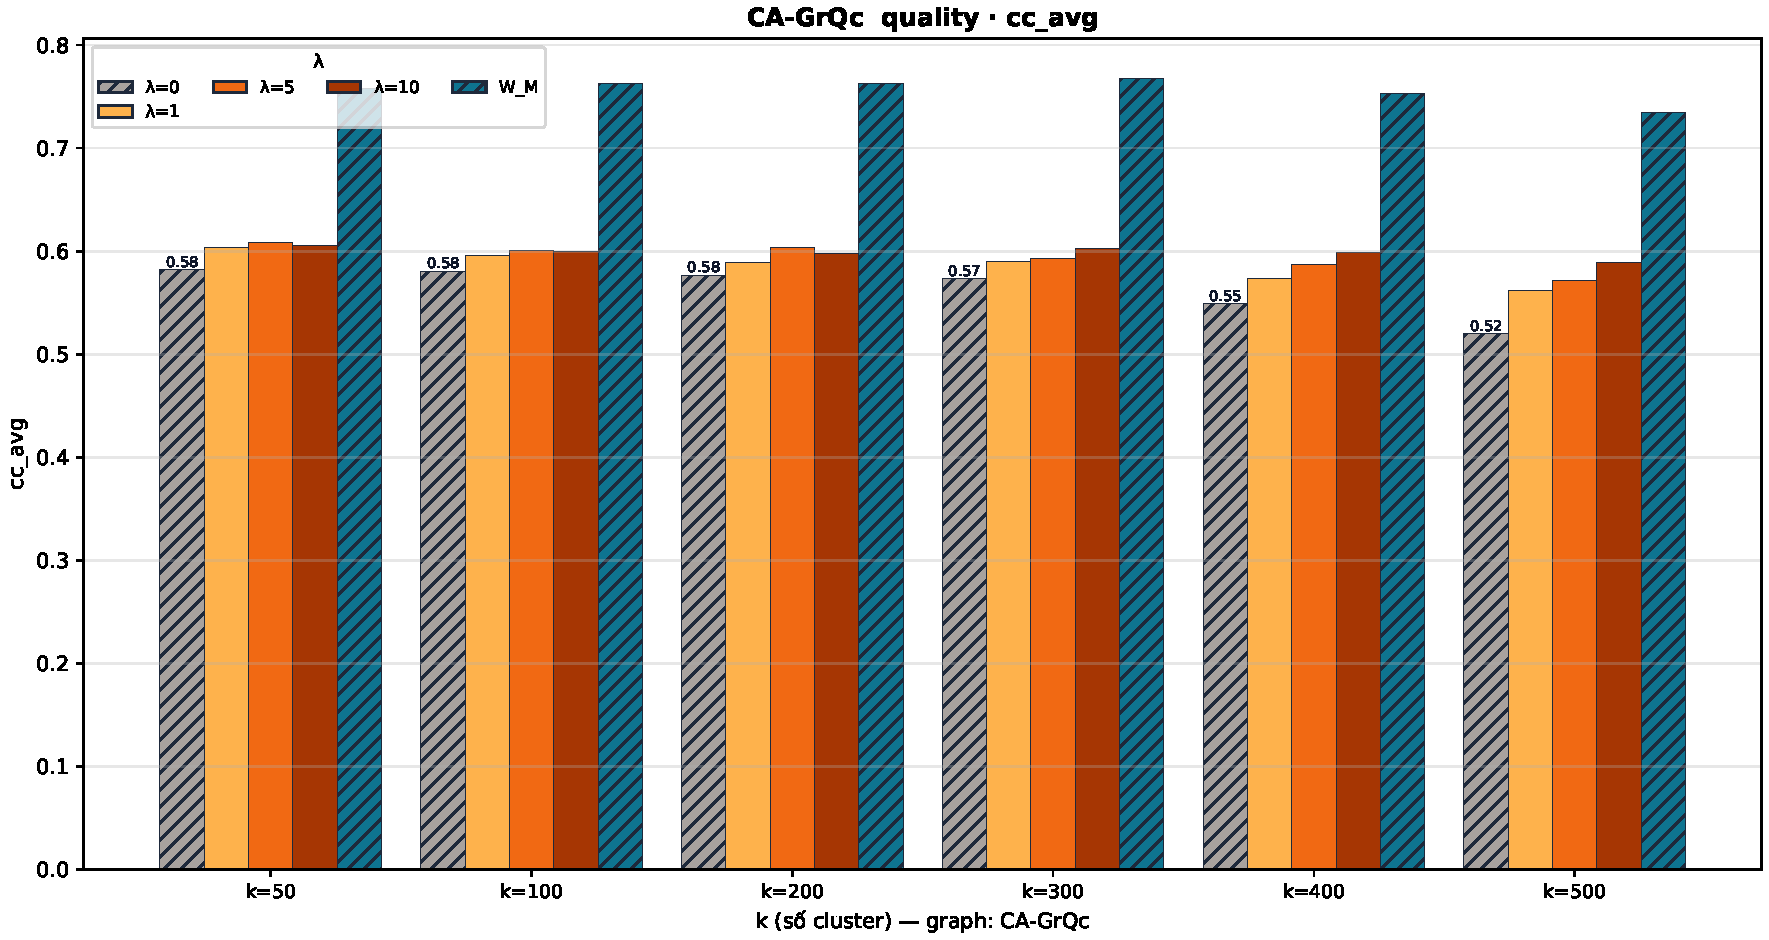
\includegraphics[width=\textwidth]{../main_result/REAL/CA-GrQc/charts/quality_cc_avg.pdf}
    \caption{$\overline{\mathrm{CC}}$ trên CA-GrQc theo $\lambda$ và $K$.}
    \label{fig:real-ccavg-grqc}
\end{figure}

Tại $K = 50$, $\overline{\mathrm{CC}}_w(0) = 0{,}5677$ sát $cc_{\mathrm{global}}$. $\overline{\mathrm{CC}}_w$ tăng nhẹ lên $0{,}6167$ tại $W_M$, biên độ điển hình của đồ thị có $cc_{\mathrm{global}}$ cao. $\overline{\mathrm{CC}}$ bật từ $0{,}6056$ tại $\lambda = 10$ lên $0{,}7574$ tại $W_M$, một bước nhảy $0{,}15$ trong khi $\overline{\mathrm{CC}}_w$ trong cùng đoạn chỉ tăng $0{,}03$. Nhóm nghiên cứu nhỏ với hệ số phân cụm gần $1$ bị $W_M$ tách ra thành cụm riêng, thiên lệch $\overline{\mathrm{CC}}$ nhưng được $\overline{\mathrm{CC}}_w$ giữ ổn định.

\textbf{Kết luận.} CA-GrQc đại diện cho mạng đồng tác giả nhỏ với cấu trúc nhóm nghiên cứu đã được phân cụm phổ trên $A$ phát hiện gần như tối ưu. Vai trò của $W_\lambda$ chỉ thể hiện khi tăng $K$ để chia nhỏ các nhóm lớn; ngược lại, cấu trúc tam giác nội cụm là đặc trưng cố hữu của đồ thị nên $\overline{\mathrm{CC}}_w$ chỉ tăng khiêm tốn.

% ............................................................
\subsection*{CA-AstroPh}

Tương tự CA-GrQc nhưng cho lĩnh vực Vật lý thiên văn. Đồ thị lớn hơn ($n = 17{,}903$) và đậm đặc tam giác hơn. Hệ số phân cụm toàn cục $cc_{\mathrm{global}} = 0{,}6328$ cao hơn CA-GrQc, do cộng tác trong vật lý thiên văn thường nhiều tác giả cùng một bài.

\textbf{Modularity.}
\begin{figure}[H]
    \centering
    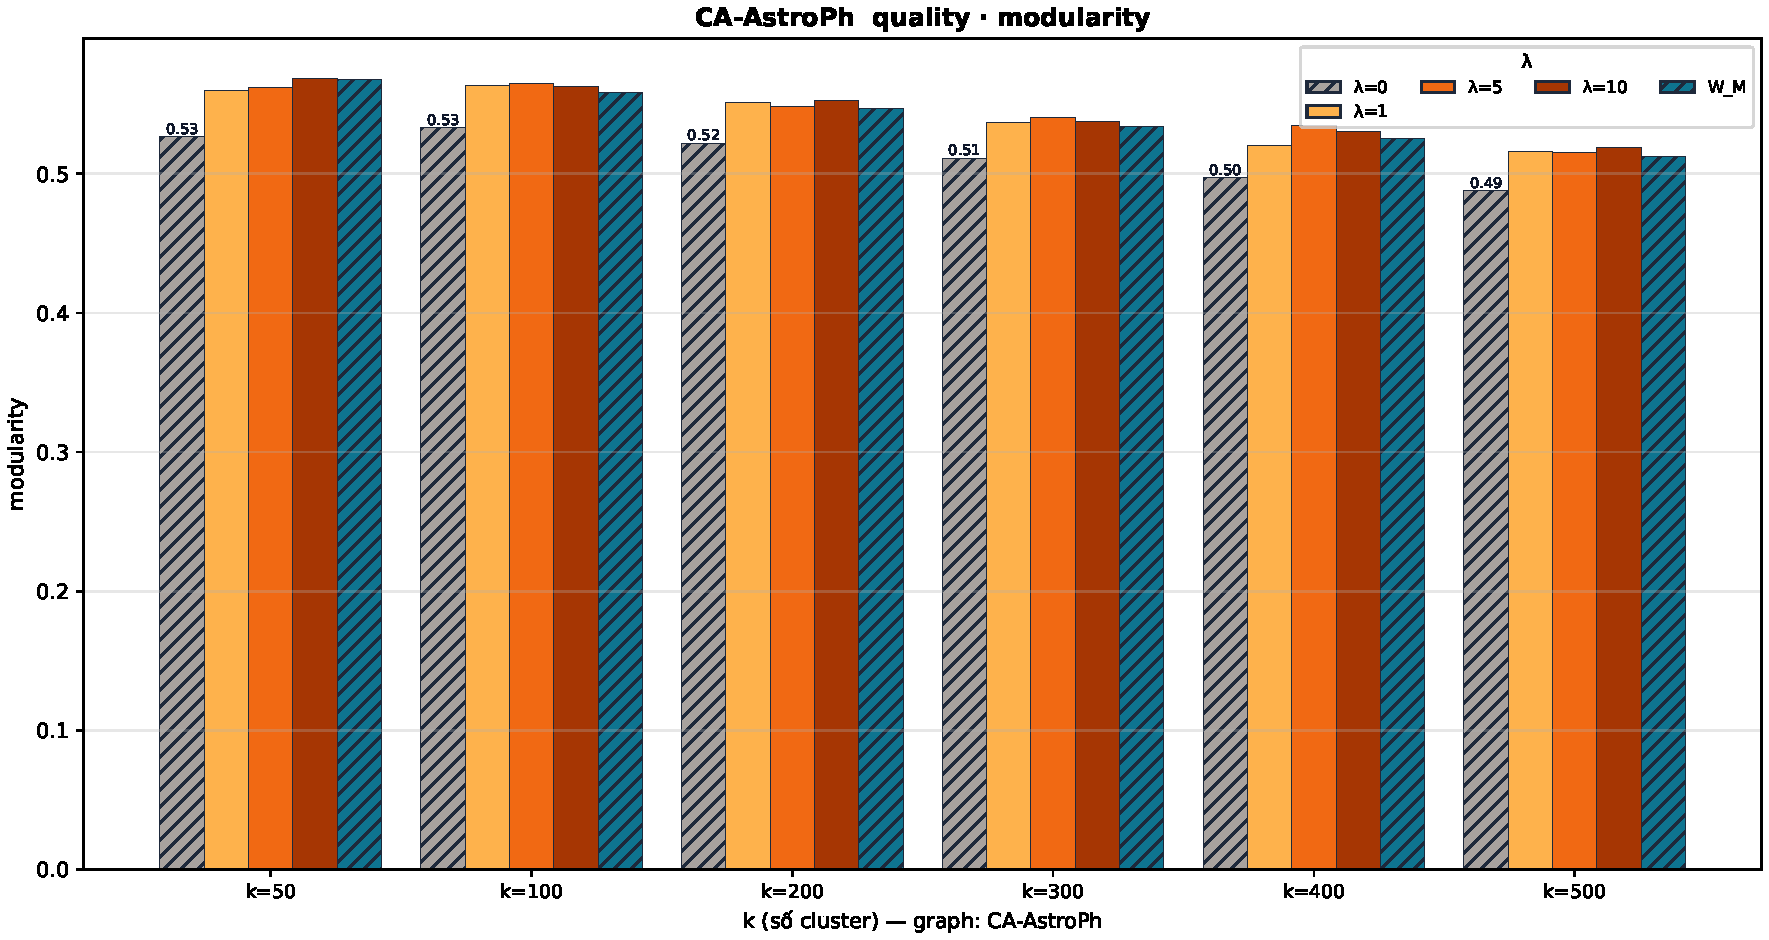
\includegraphics[width=\textwidth]{../main_result/REAL/CA-AstroPh/charts/quality_modularity.pdf}
    \caption{Modularity $Q$ trên CA-AstroPh theo $\lambda$ và $K$.}
    \label{fig:real-astroph}
\end{figure}

$Q(0)$ tập trung ở vùng $0{,}49$--$0{,}53$, cải thiện đồng đều $+0{,}030$ đến $+0{,}042$. Tại $K = 50$, $\Delta Q = +0{,}0421$ với $\lambda^* = 10$. Đồ thị không có bộ test nào ở vùng $Q(0)$ cao nên biên độ $\Delta Q$ không bị thu hẹp như CA-GrQc.

\textbf{Hệ số phân cụm.}
\begin{figure}[H]
    \centering
    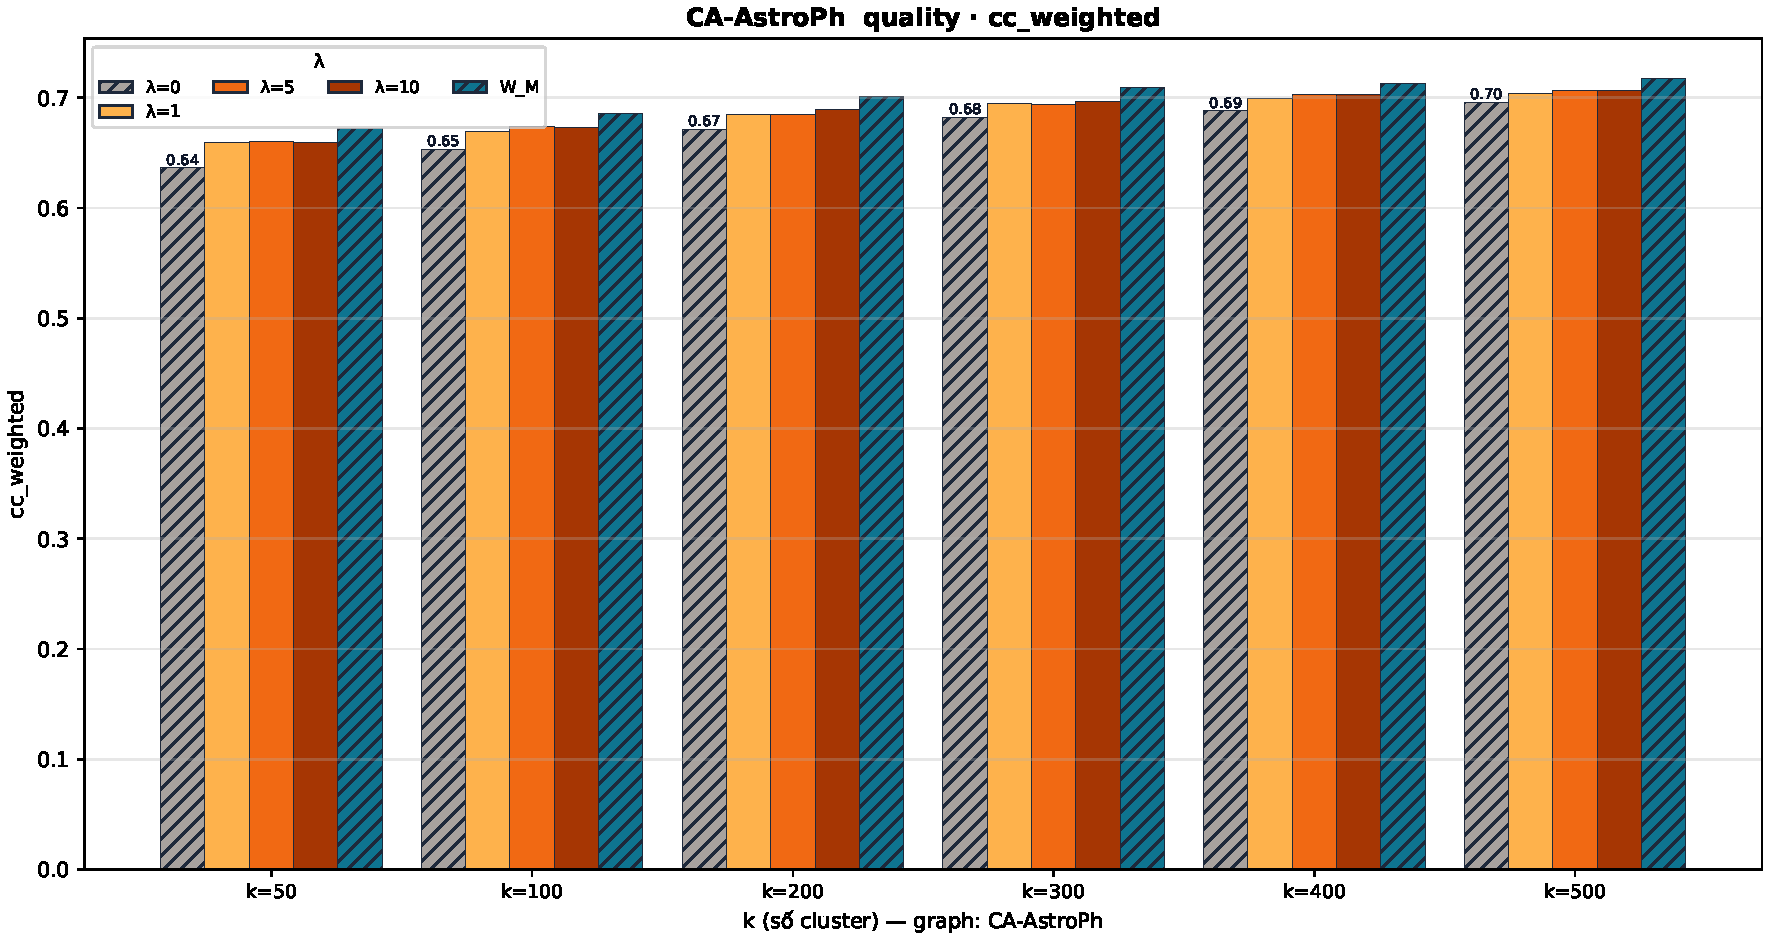
\includegraphics[width=\textwidth]{../main_result/REAL/CA-AstroPh/charts/quality_cc_weighted.pdf}
    \caption{$\overline{\mathrm{CC}}_w$ trên CA-AstroPh theo $\lambda$ và $K$.}
    \label{fig:real-cc-astroph}
\end{figure}

\begin{figure}[H]
    \centering
    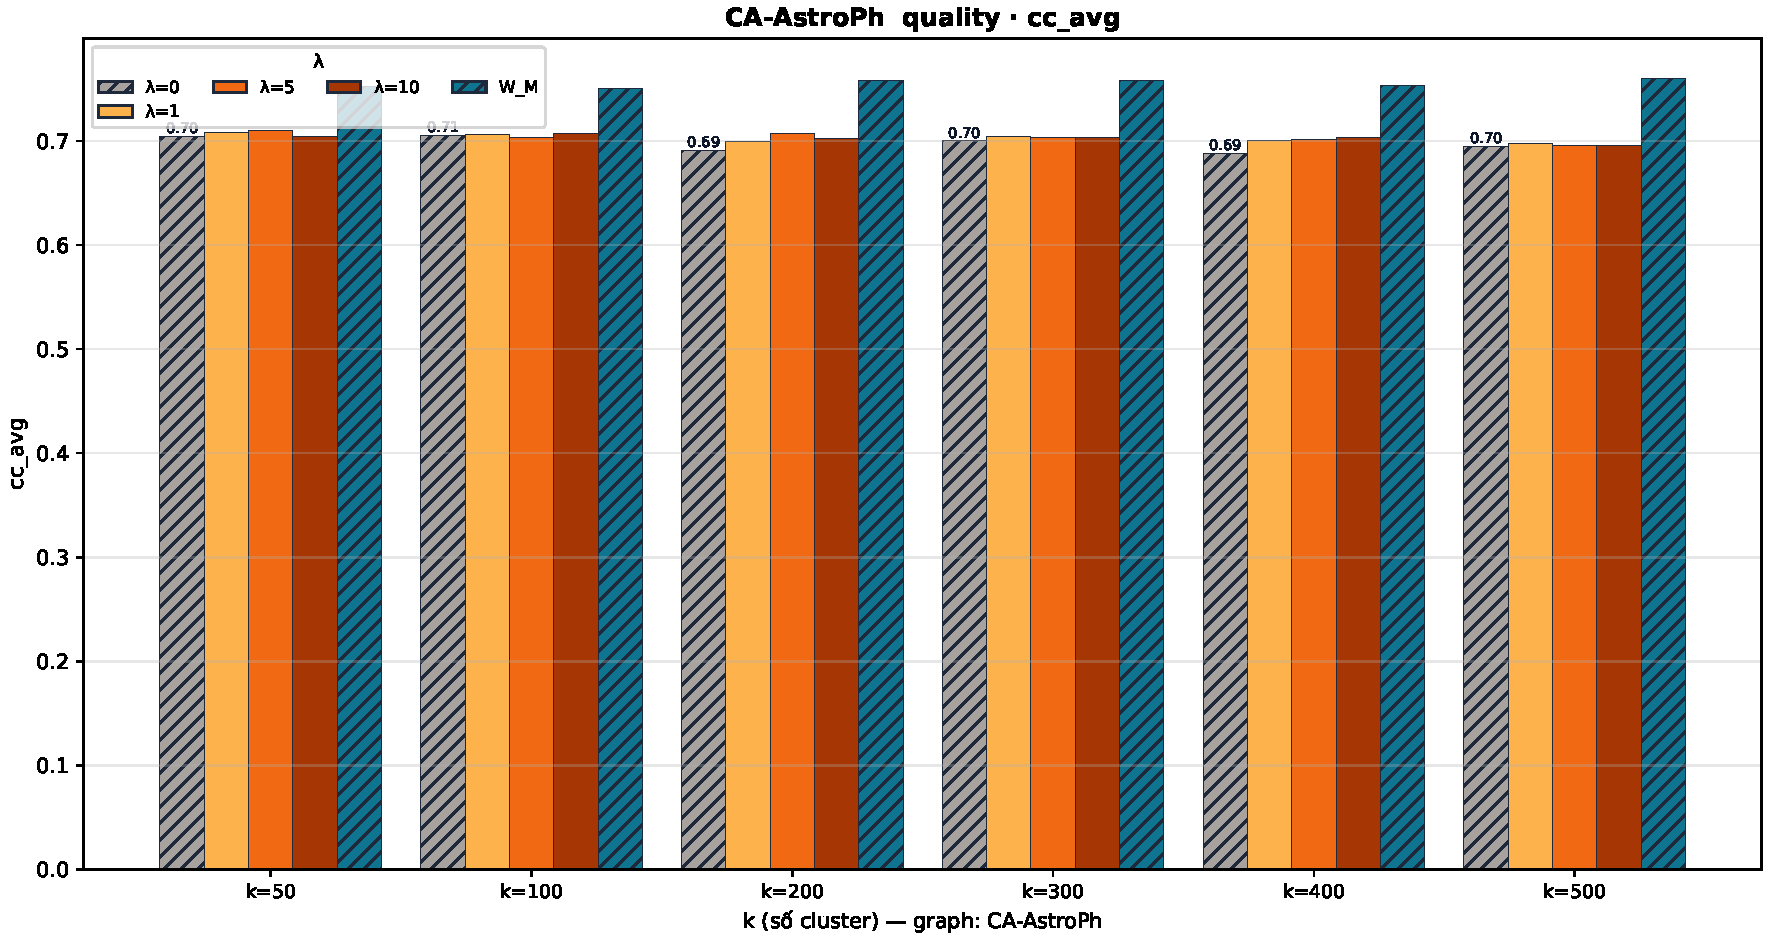
\includegraphics[width=\textwidth]{../main_result/REAL/CA-AstroPh/charts/quality_cc_avg.pdf}
    \caption{$\overline{\mathrm{CC}}$ trên CA-AstroPh theo $\lambda$ và $K$.}
    \label{fig:real-ccavg-astroph}
\end{figure}

Tại $K = 50$, $\overline{\mathrm{CC}}_w(0) = 0{,}6365$ trùng khớp với $cc_{\mathrm{global}}$. $\overline{\mathrm{CC}}_w$ tăng nhẹ lên $0{,}6717$ tại $W_M$. $\overline{\mathrm{CC}}$ bật từ $0{,}7041$ tại $\lambda = 10$ lên $0{,}7518$ tại $W_M$, chênh $0{,}08$ so với $\overline{\mathrm{CC}}_w$. Bứt phá $\overline{\mathrm{CC}}$ tại $W_M$ vừa phải do CA-AstroPh là đồ thị lớn với nhiều nhóm hợp tác có kích thước trung bình, ít cụm cực nhỏ.

\textbf{Kết luận.} CA-AstroPh thuộc nhóm đồ thị đồng tác giả lớn với $cc_{\mathrm{global}}$ cao và phân hoạch ban đầu chất lượng trung bình. Vai trò của $W_\lambda$ chủ yếu là tinh chỉnh modularity, không tạo ra thay đổi cấu trúc tam giác đáng kể.

% ............................................................
\subsection*{CA-CondMat}

Tương tự CA-GrQc nhưng cho lĩnh vực Vật chất ngưng tụ. Hệ số phân cụm toàn cục $cc_{\mathrm{global}} = 0{,}6417$ rất cao, gần với CA-AstroPh.

\textbf{Modularity.}
\begin{figure}[H]
    \centering
    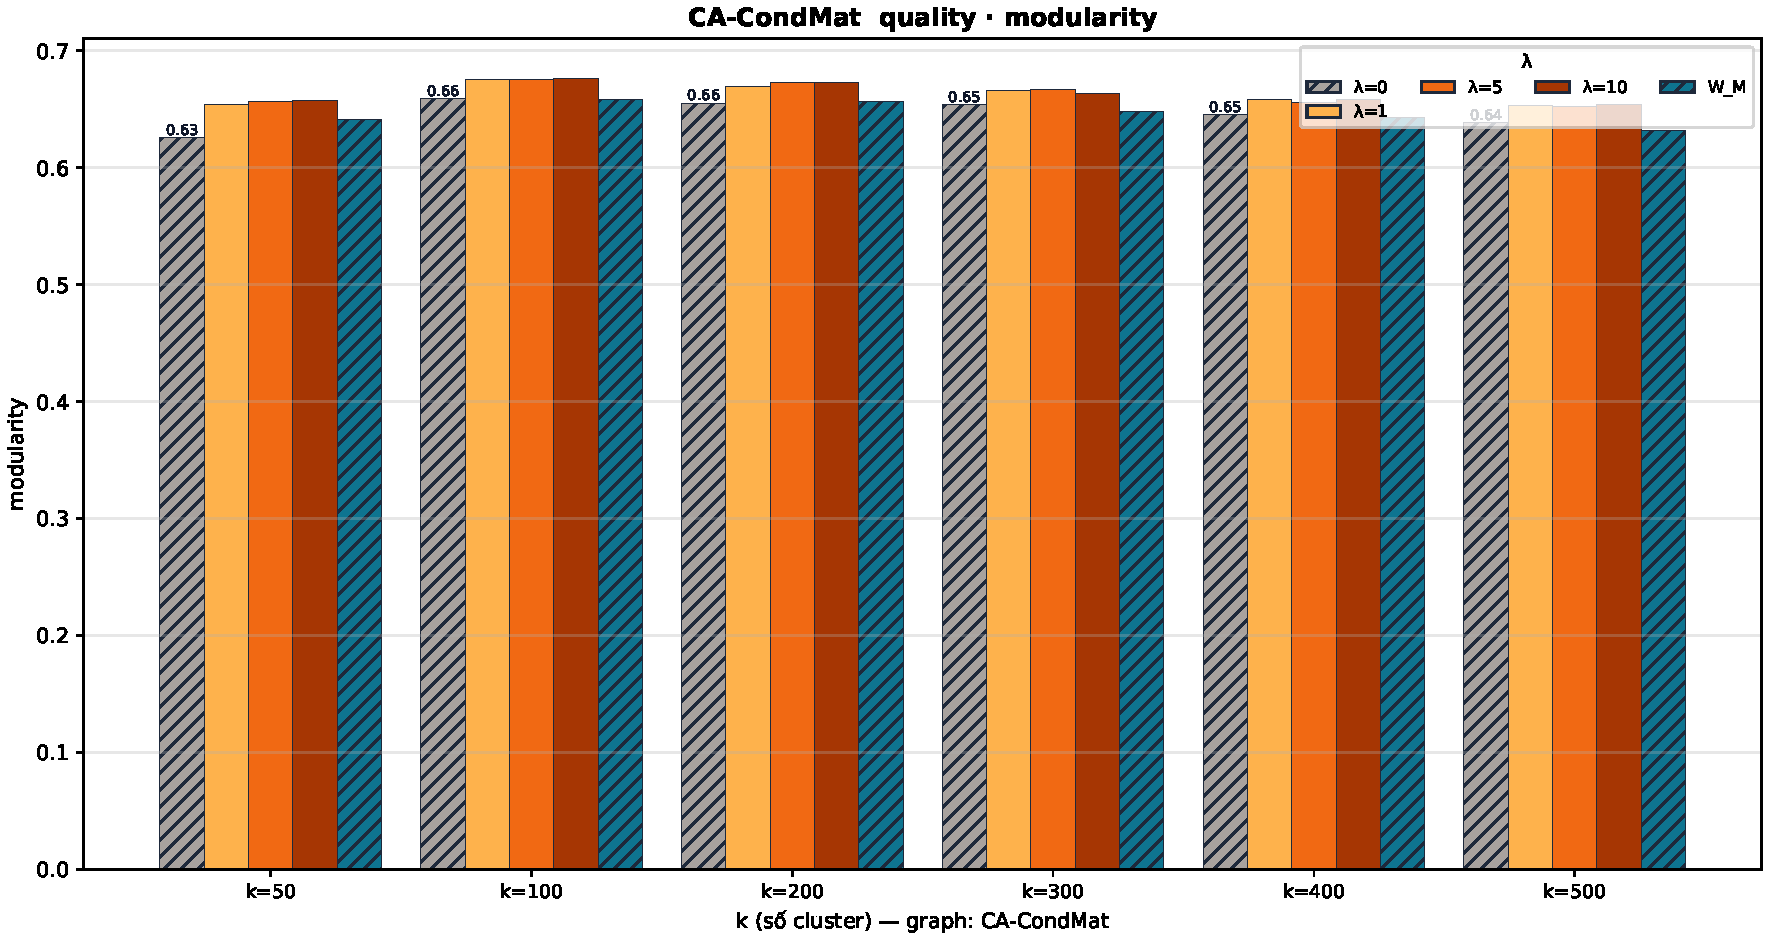
\includegraphics[width=\textwidth]{../main_result/REAL/CA-CondMat/charts/quality_modularity.pdf}
    \caption{Modularity $Q$ trên CA-CondMat theo $\lambda$ và $K$.}
    \label{fig:real-condmat}
\end{figure}

$Q(0)$ cao trên toàn dải ($0{,}62$--$0{,}66$). $\Delta Q$ nhỏ, dao động từ $+0{,}013$ đến $+0{,}032$. Tại $K = 50$, $\Delta Q = +0{,}0316$ với $\lambda^* = 10$. Khi $Q(0)$ đã gần đạt mức cao của thang $Q$, biên độ cải thiện khả dĩ vốn nhỏ nên $\Delta Q$ bị thu hẹp.

\textbf{Hệ số phân cụm.}
\begin{figure}[H]
    \centering
    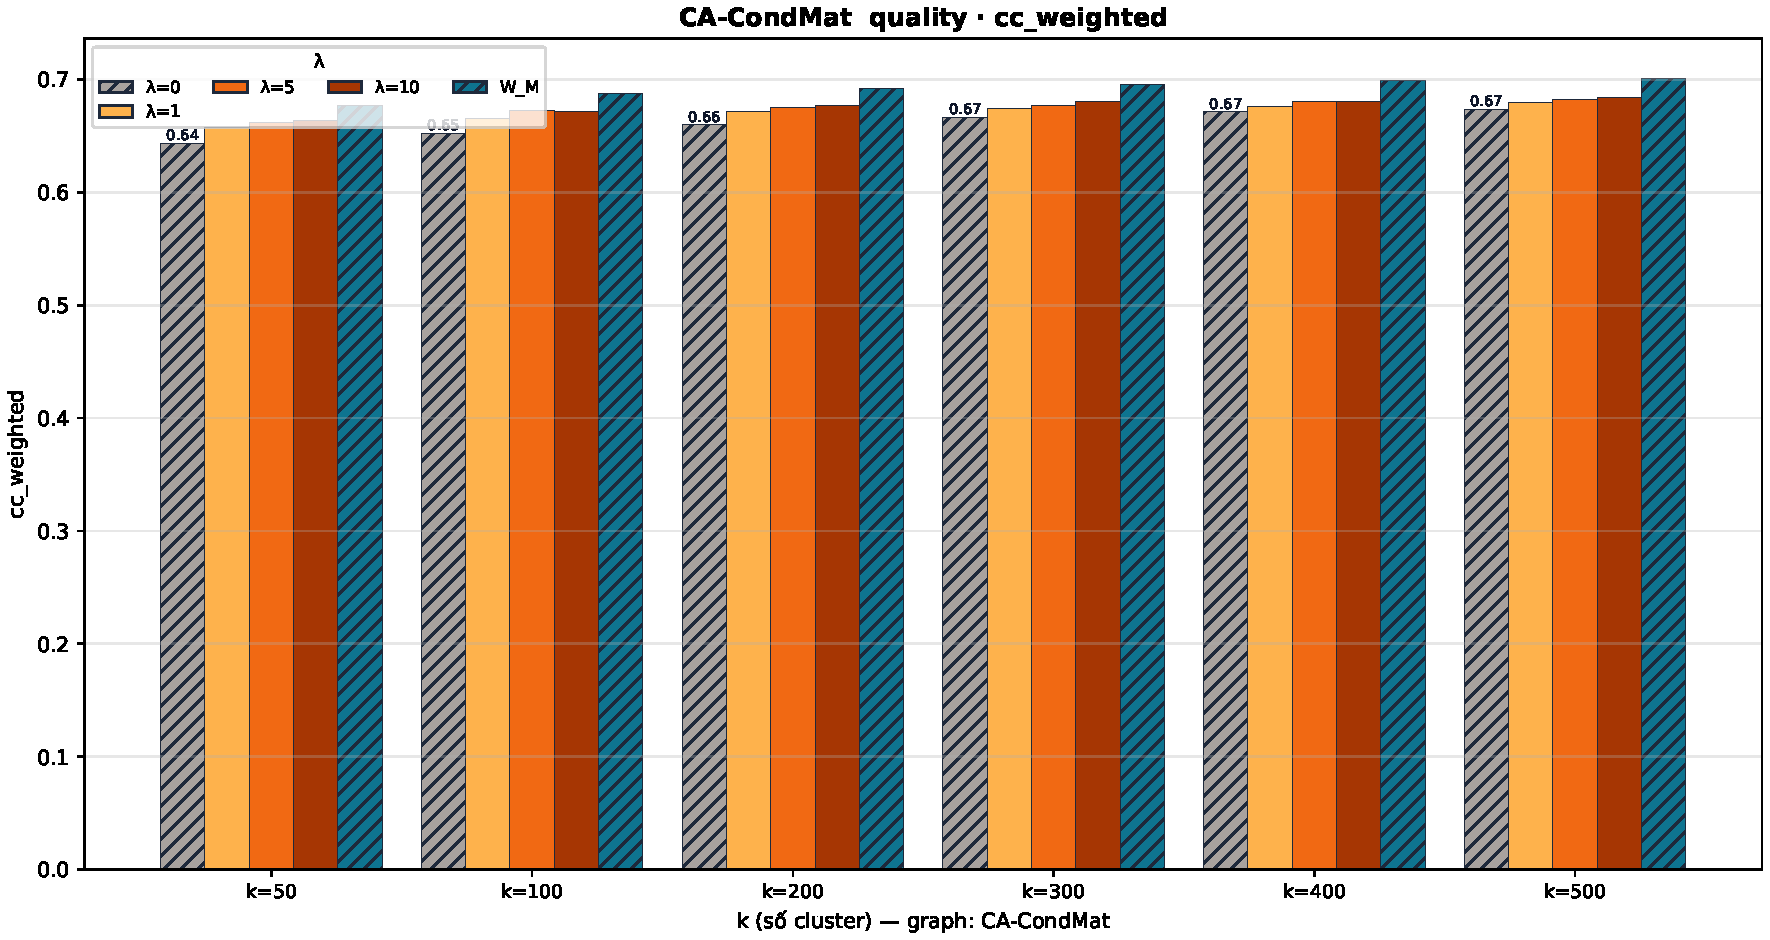
\includegraphics[width=\textwidth]{../main_result/REAL/CA-CondMat/charts/quality_cc_weighted.pdf}
    \caption{$\overline{\mathrm{CC}}_w$ trên CA-CondMat theo $\lambda$ và $K$.}
    \label{fig:real-cc-condmat}
\end{figure}

\begin{figure}[H]
    \centering
    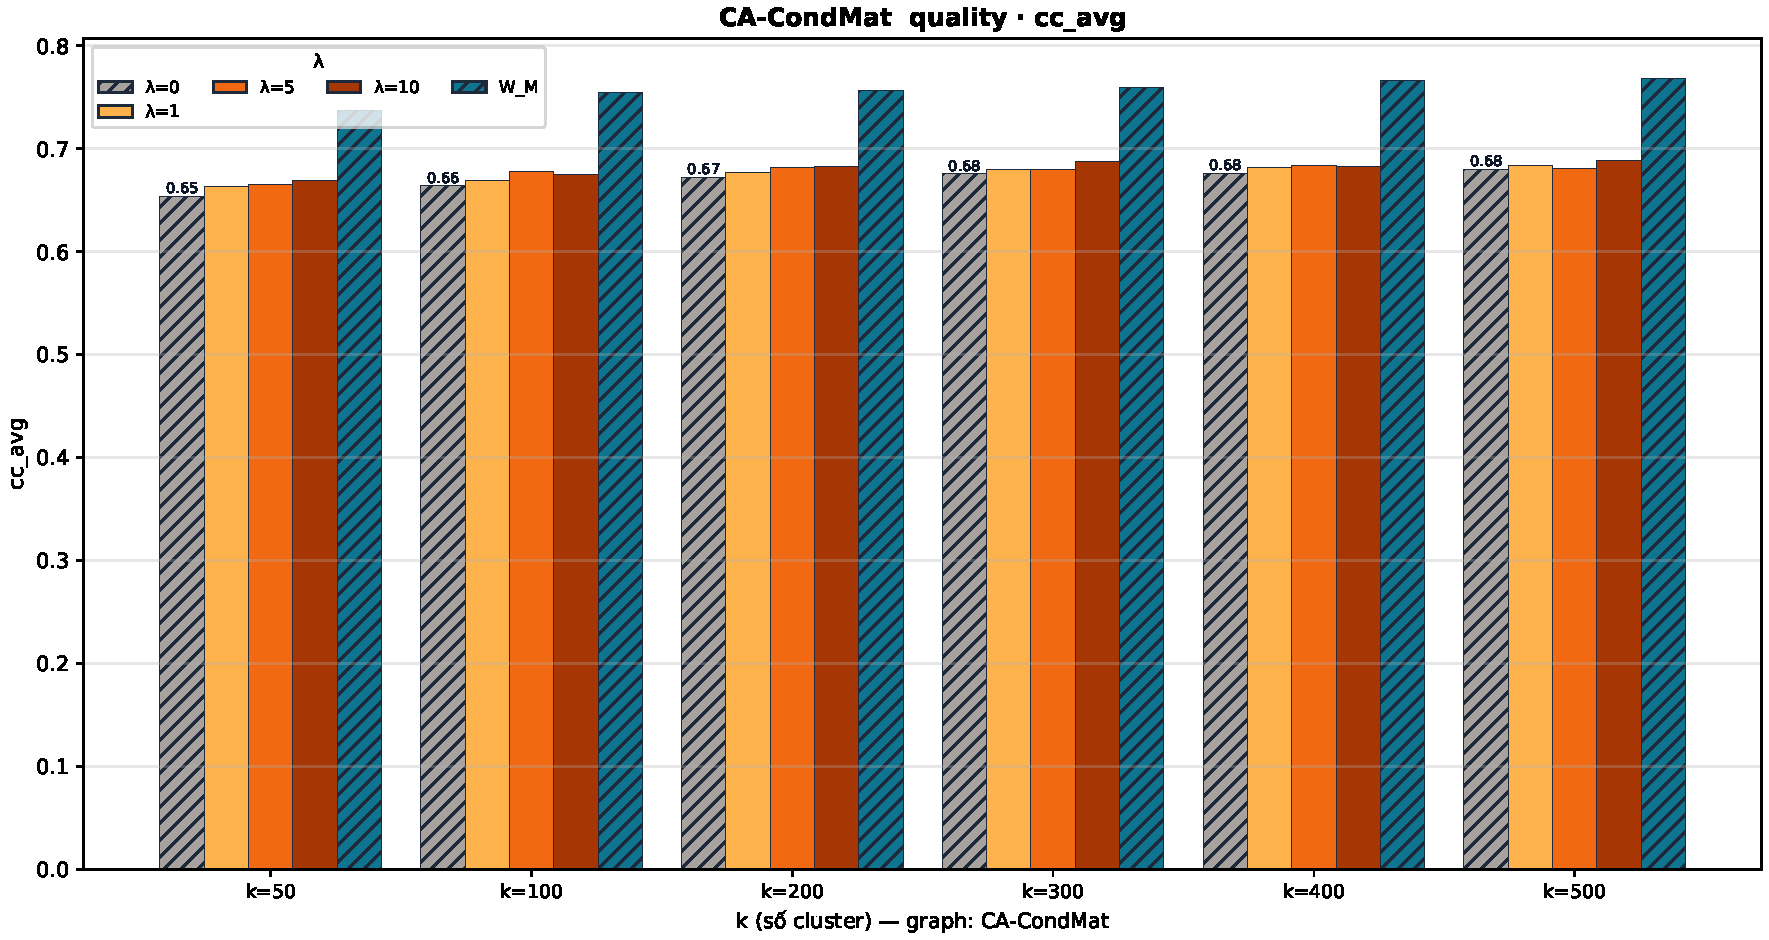
\includegraphics[width=\textwidth]{../main_result/REAL/CA-CondMat/charts/quality_cc_avg.pdf}
    \caption{$\overline{\mathrm{CC}}$ trên CA-CondMat theo $\lambda$ và $K$.}
    \label{fig:real-ccavg-condmat}
\end{figure}

Tại $K = 50$, $\overline{\mathrm{CC}}_w(0) = 0{,}6435$ trùng $cc_{\mathrm{global}}$. Tăng lên $0{,}6769$ tại $W_M$. $\overline{\mathrm{CC}}$ bật từ $0{,}6691$ tại $\lambda = 10$ lên $0{,}7370$ tại $W_M$ (tăng $0{,}07$), trong khi $\overline{\mathrm{CC}}_w$ chỉ tăng $0{,}01$ trong cùng đoạn. Phân mảnh cụm tại $W_M$ ở mức khiêm tốn, $\overline{\mathrm{CC}}_w$ giữ ổn định phản ánh đúng kích thước cụm.

\textbf{Kết luận.} CA-CondMat tái lập pattern của CA-AstroPh và CA-GrQc: mạng đồng tác giả có cấu trúc tam giác mạnh đã được phân cụm phổ trên $A$ khai thác gần tối ưu, $W_\lambda$ chỉ đóng vai trò tinh chỉnh.

% ............................................................
\subsection*{CA-HepTh}

Tương tự CA-GrQc nhưng cho lĩnh vực Vật lý năng lượng cao lý thuyết. Đồ thị đồng tác giả thưa nhất trong nhóm CA-, hệ số phân cụm toàn cục $cc_{\mathrm{global}} = 0{,}4816$ thấp nhất nhóm.

\textbf{Modularity.}
\begin{figure}[H]
    \centering
    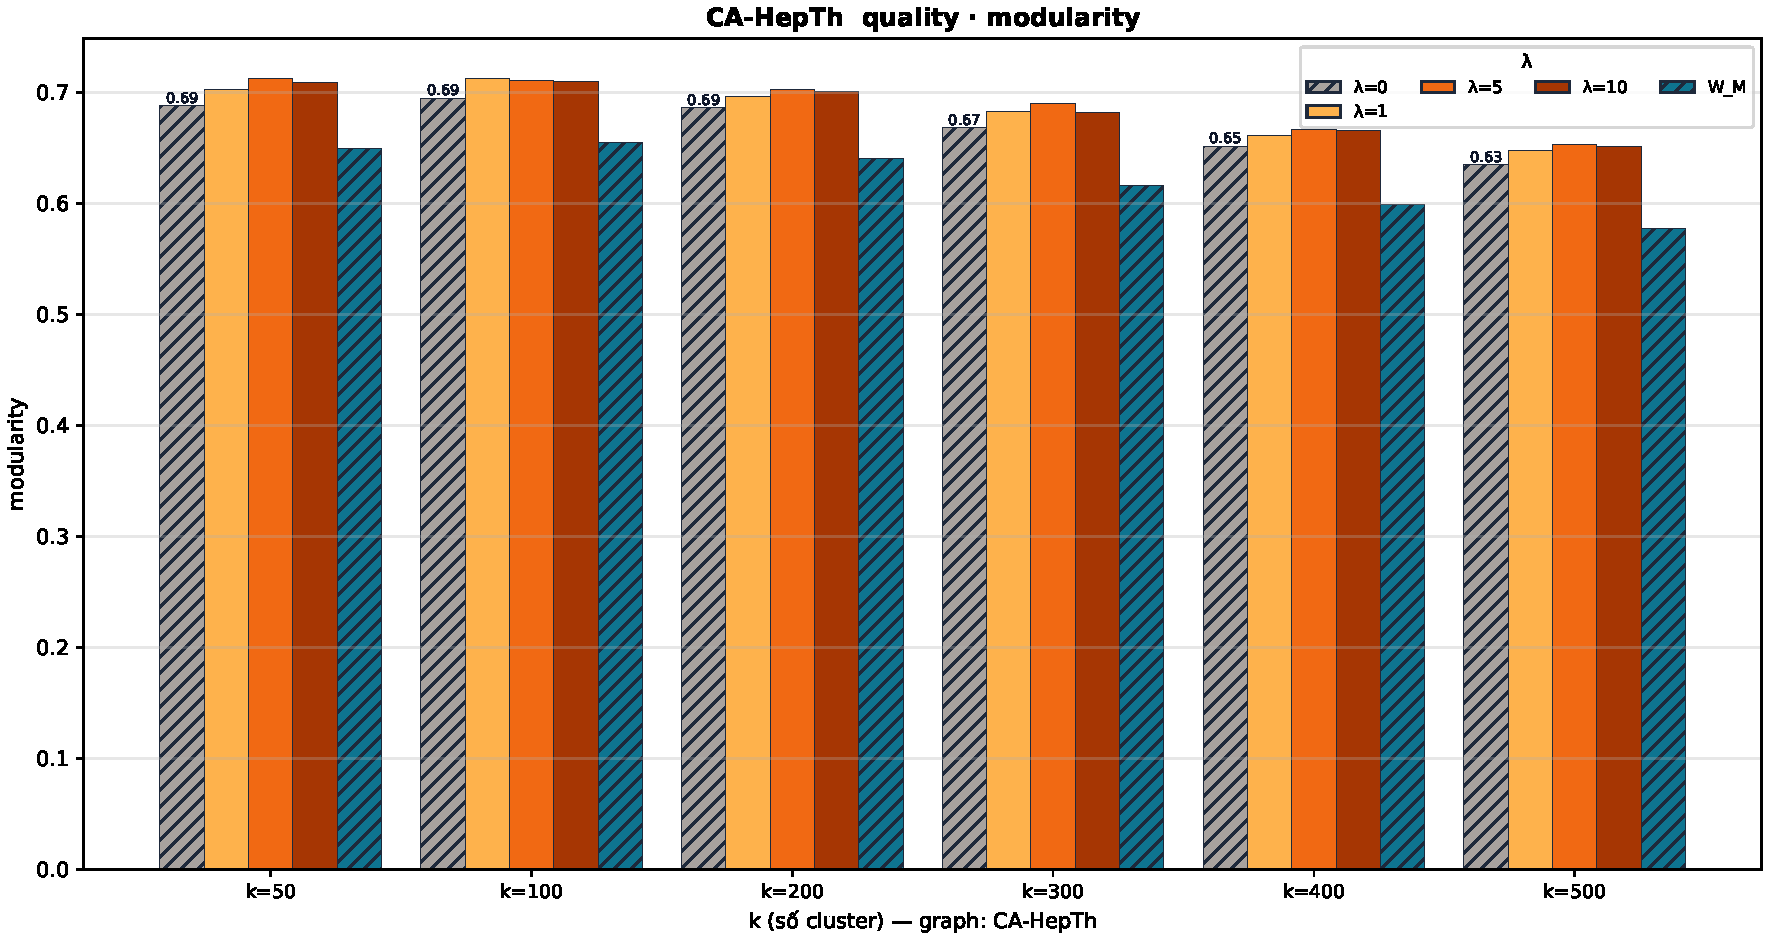
\includegraphics[width=\textwidth]{../main_result/REAL/CA-HepTh/charts/quality_modularity.pdf}
    \caption{Modularity $Q$ trên CA-HepTh theo $\lambda$ và $K$.}
    \label{fig:real-hepth}
\end{figure}

$Q(0)$ cao ($0{,}63$--$0{,}69$). $\Delta Q$ chỉ $+0{,}015$ đến $+0{,}025$, mức cải thiện không đáng kể nhưng đều dương. Tại $K = 50$, $\Delta Q = +0{,}0250$ với $\lambda^* = 5$. Khẳng định thêm xu hướng $\Delta Q$ thu hẹp khi $Q(0)$ đã cao.

\textbf{Hệ số phân cụm.}
\begin{figure}[H]
    \centering
    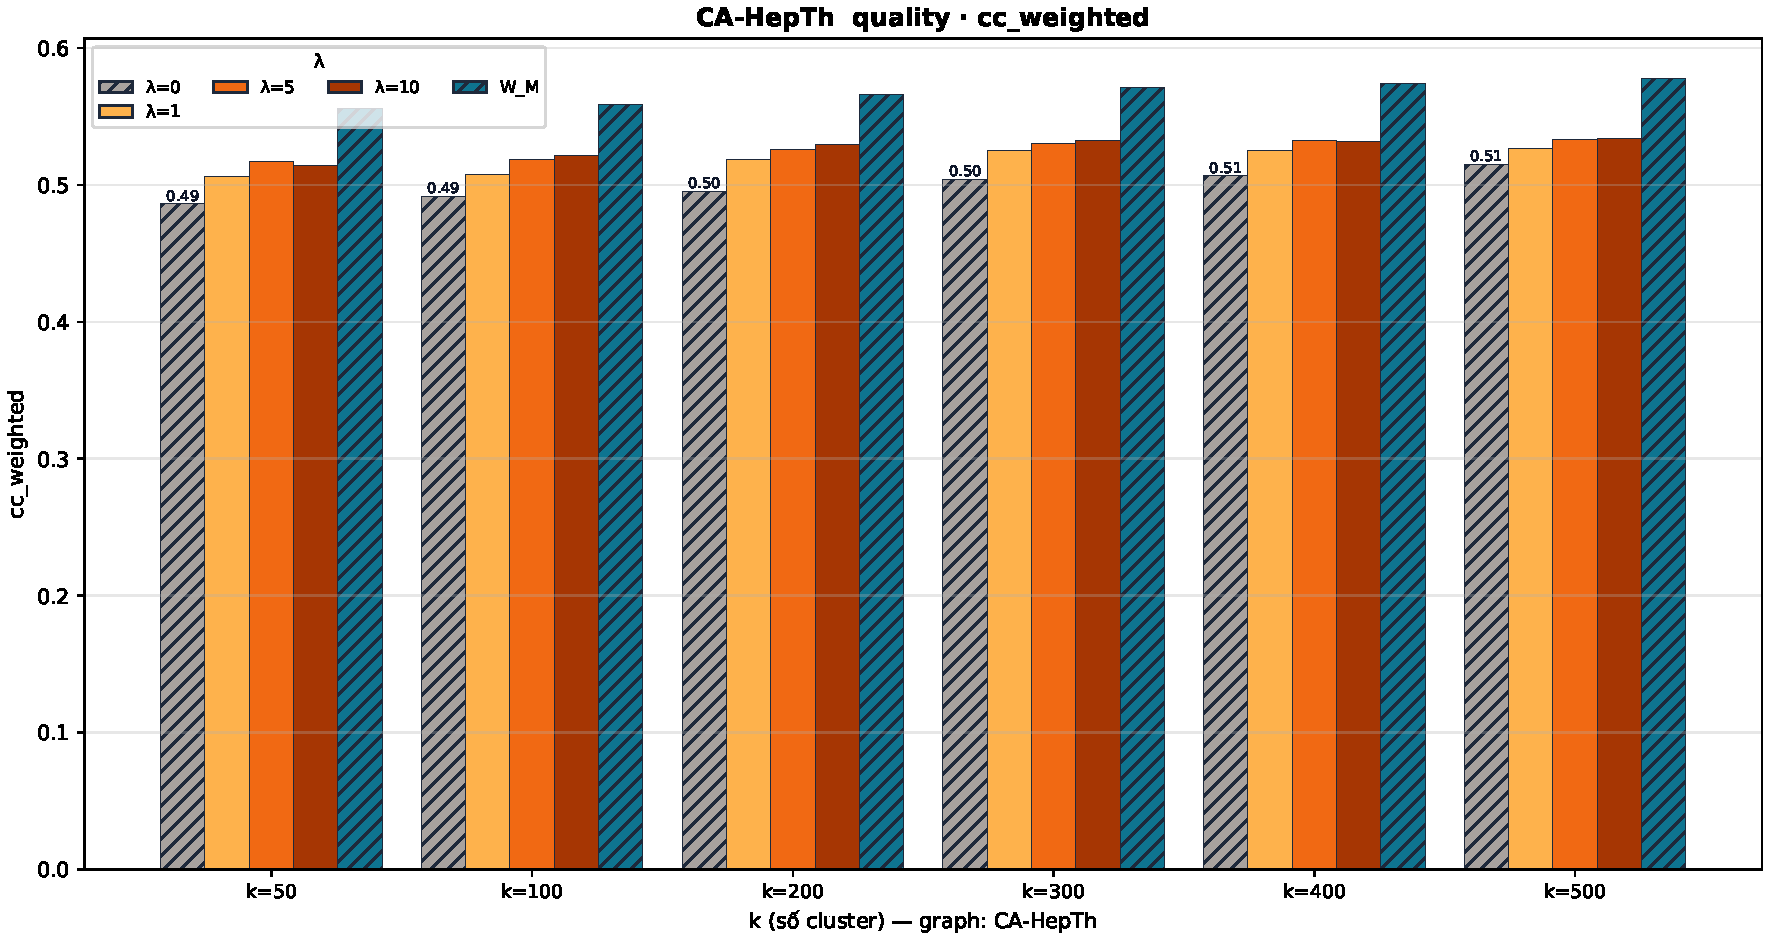
\includegraphics[width=\textwidth]{../main_result/REAL/CA-HepTh/charts/quality_cc_weighted.pdf}
    \caption{$\overline{\mathrm{CC}}_w$ trên CA-HepTh theo $\lambda$ và $K$.}
    \label{fig:real-cc-hepth}
\end{figure}

\begin{figure}[H]
    \centering
    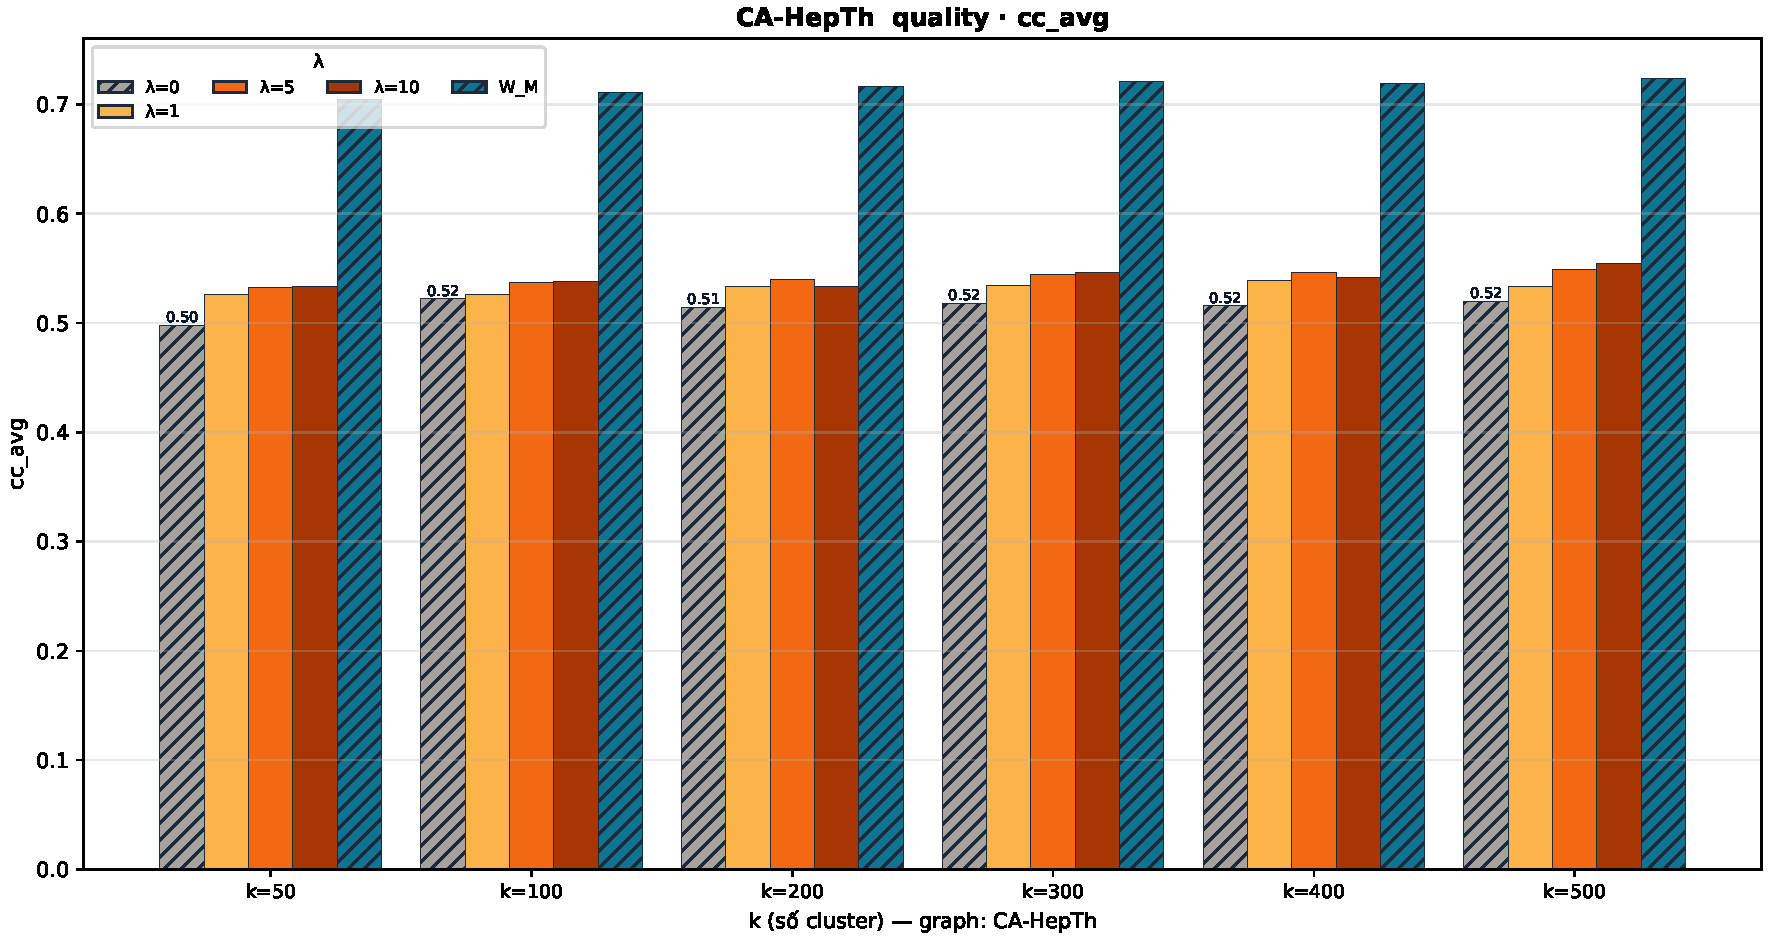
\includegraphics[width=\textwidth]{../main_result/REAL/CA-HepTh/charts/quality_cc_avg.pdf}
    \caption{$\overline{\mathrm{CC}}$ trên CA-HepTh theo $\lambda$ và $K$.}
    \label{fig:real-ccavg-hepth}
\end{figure}

Tại $K = 50$, $\overline{\mathrm{CC}}_w(0) = 0{,}4863$ sát $cc_{\mathrm{global}}$, tăng lên $0{,}5557$ tại $W_M$. $\overline{\mathrm{CC}}$ bật từ $0{,}5337$ tại $\lambda = 10$ lên $0{,}7043$ tại $W_M$, tăng $0{,}17$ chỉ qua một bước trong khi $\overline{\mathrm{CC}}_w$ trong cùng đoạn tăng $0{,}04$. Chênh lệch $0{,}15$ giữa hai đại lượng tại $W_M$ là một trong những chênh lớn nhất trong tập dữ liệu thật, dấu hiệu CA-HepTh có nhiều nhóm nghiên cứu thưa cỡ nhỏ bị $W_M$ tách rời.

\textbf{Kết luận.} CA-HepTh là phiên bản thưa của họ CA-, modularity sớm đạt mức cao nên biên độ cải thiện theo $Q$ nhỏ, nhưng $\overline{\mathrm{CC}}_w$ vẫn có khoảng cải thiện đáng kể. Chênh lớn giữa $\overline{\mathrm{CC}}$ và $\overline{\mathrm{CC}}_w$ phản ánh nhiều nhóm nghiên cứu nhỏ với hệ số phân cụm gần $1$.

% ............................................................
\subsection*{musae\_facebook}

Đỉnh là một trang Facebook công khai, cạnh nối hai trang có liên kết ``like'' lẫn nhau. Cộng đồng phản ánh chủ đề hoặc lĩnh vực của trang. Hệ số phân cụm toàn cục $cc_{\mathrm{global}} = 0{,}3597$, thấp hơn các mạng xã hội cá nhân do quan hệ ``like'' giữa trang phản ánh chủ đề hơn là cộng tác ba bên.

\textbf{Modularity.}
\begin{figure}[H]
    \centering
    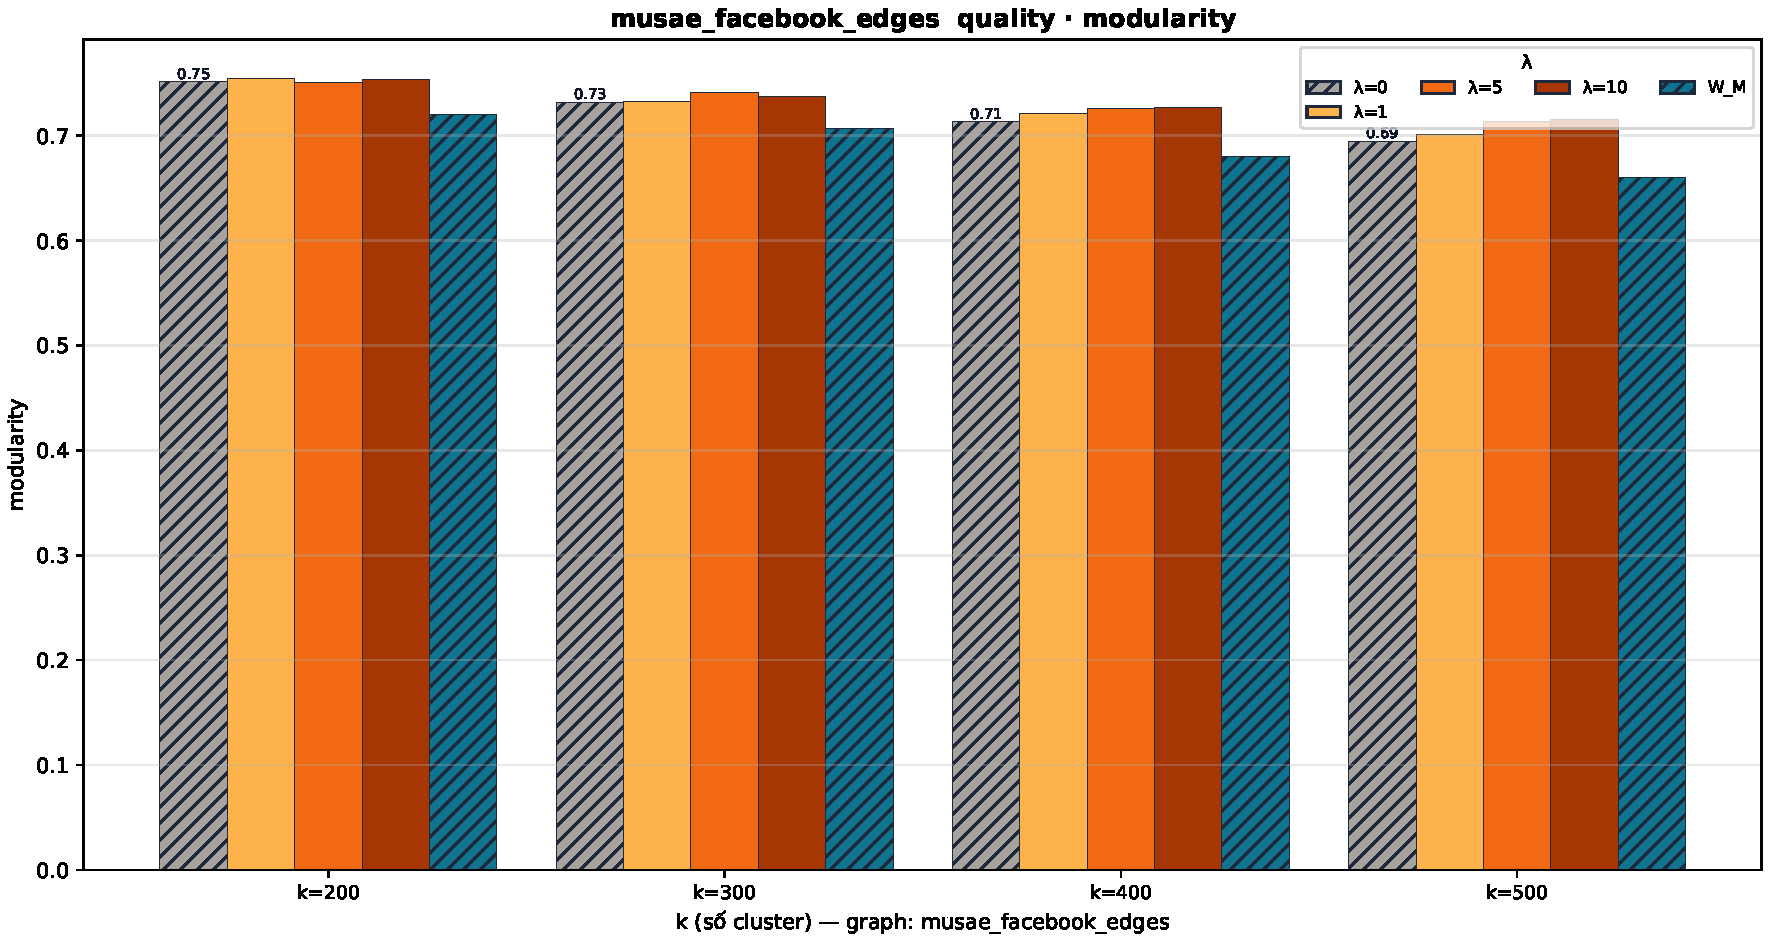
\includegraphics[width=\textwidth]{../main_result/REAL/musae_facebook_edges/charts/quality_modularity.pdf}
    \caption{Modularity $Q$ trên musae\_facebook theo $\lambda$ và $K$.}
    \label{fig:real-musae-fb}
\end{figure}

$Q(0)$ rất cao ($0{,}69$--$0{,}75$). $\Delta Q$ chỉ $+0{,}003$ đến $+0{,}020$, hầu như không thay đổi kết quả phân cụm. Tại $K = 500$, $\Delta Q = +0{,}0202$ với $\lambda^* = 10$. Đây là minh chứng rõ nhất cho xu hướng $\Delta Q$ thu hẹp khi $Q(0)$ đã cao.

\textbf{Hệ số phân cụm.}
\begin{figure}[H]
    \centering
    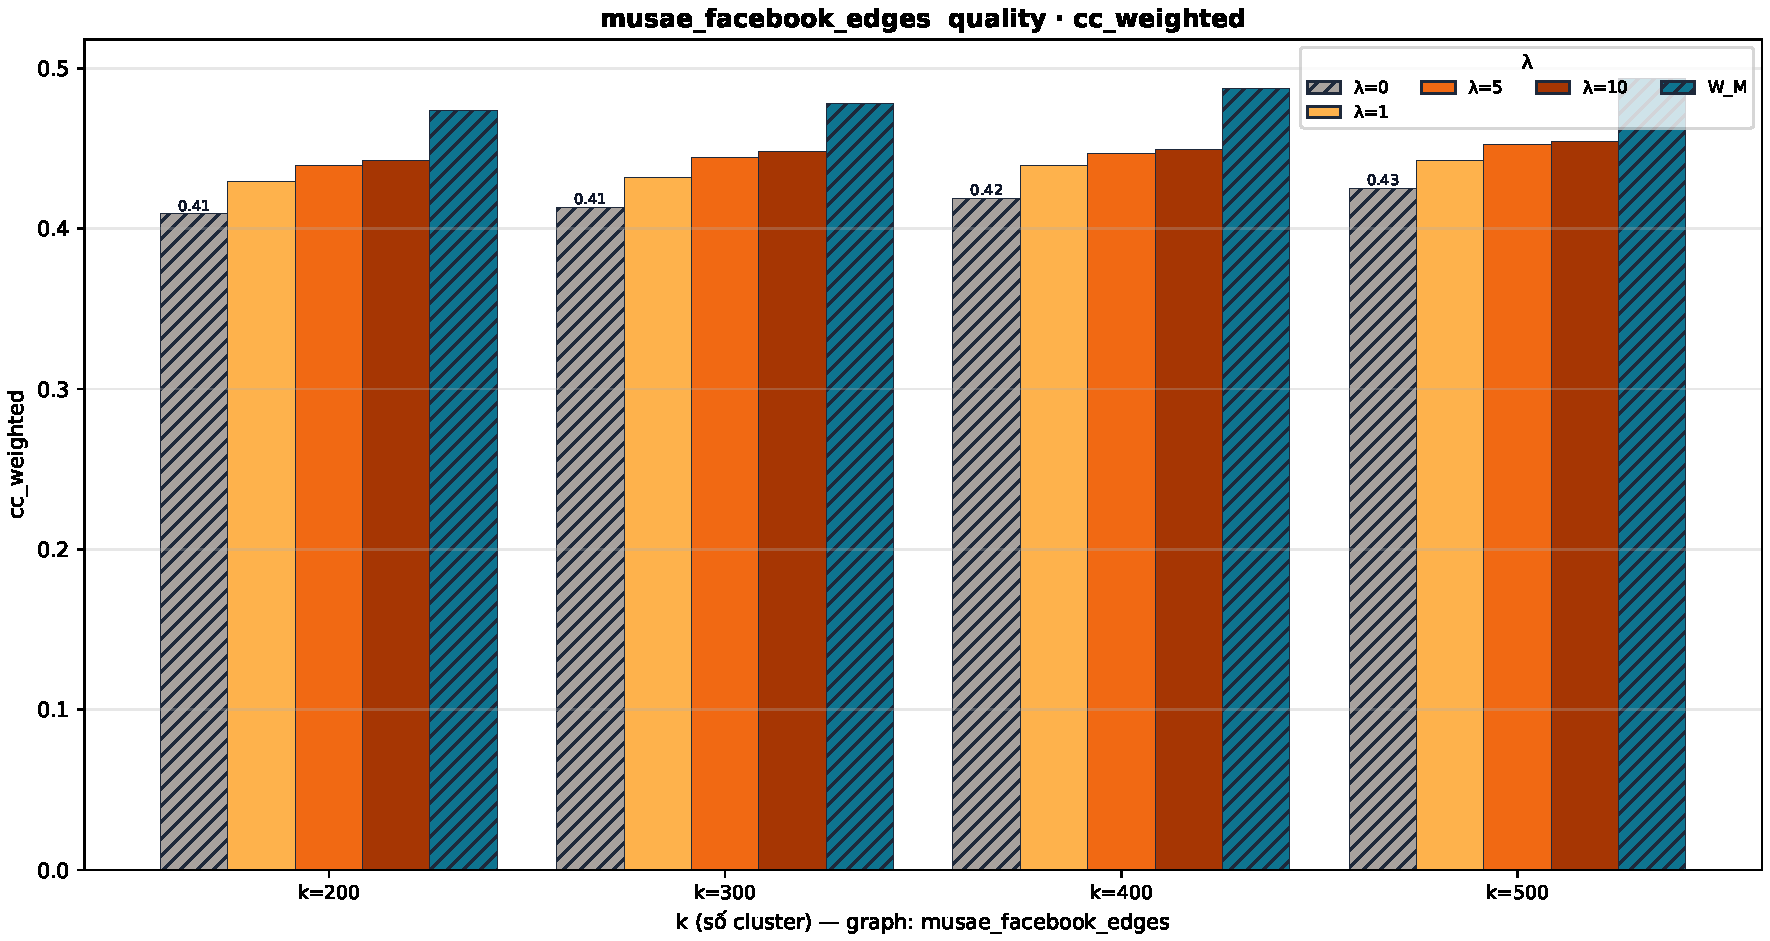
\includegraphics[width=\textwidth]{../main_result/REAL/musae_facebook_edges/charts/quality_cc_weighted.pdf}
    \caption{$\overline{\mathrm{CC}}_w$ trên musae\_facebook theo $\lambda$ và $K$.}
    \label{fig:real-cc-musae-fb}
\end{figure}

\begin{figure}[H]
    \centering
    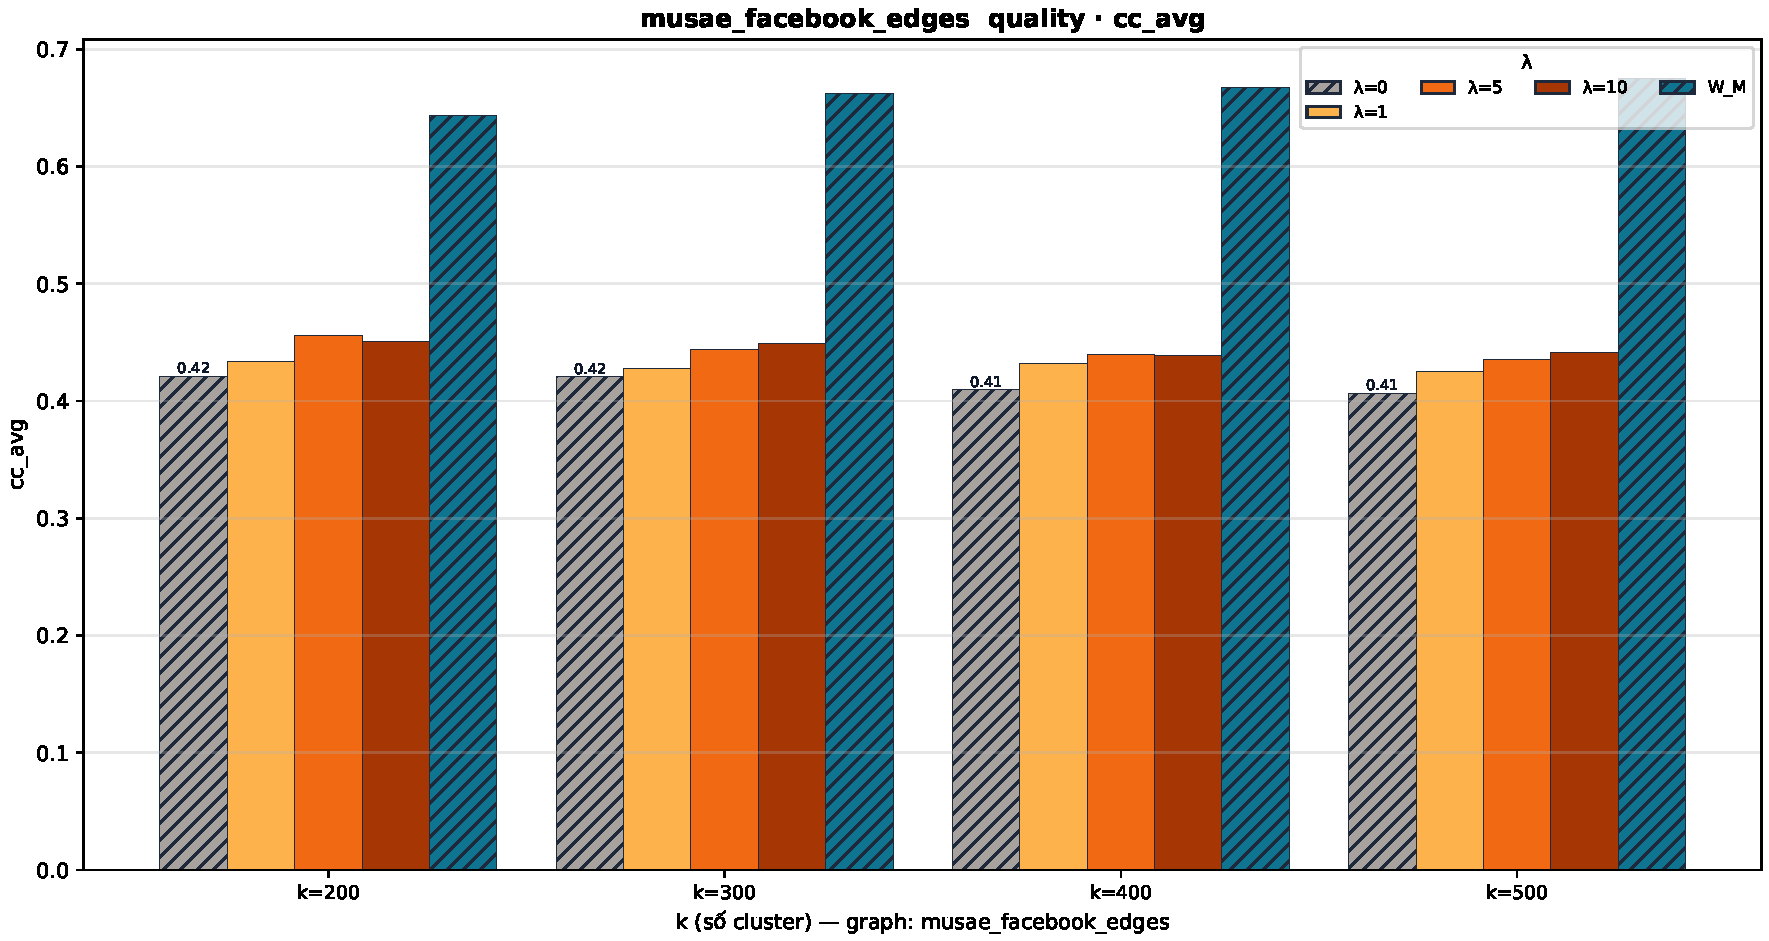
\includegraphics[width=\textwidth]{../main_result/REAL/musae_facebook_edges/charts/quality_cc_avg.pdf}
    \caption{$\overline{\mathrm{CC}}$ trên musae\_facebook theo $\lambda$ và $K$.}
    \label{fig:real-ccavg-musae-fb}
\end{figure}

Tại $K = 200$, $\overline{\mathrm{CC}}_w(0) = 0{,}4091$ đã vượt $cc_{\mathrm{global}}$, dấu hiệu phân cụm phổ trên $A$ đặt được tam giác có sẵn vào trong cụm. $\overline{\mathrm{CC}}_w$ tăng lên $0{,}4737$ tại $W_M$. $\overline{\mathrm{CC}}$ bật từ $0{,}4508$ tại $\lambda = 10$ lên $0{,}6439$ tại $W_M$, tăng $0{,}19$ trong khi $\overline{\mathrm{CC}}_w$ trong cùng đoạn tăng $0{,}03$. Chênh $0{,}17$ giữa hai đại lượng tại $W_M$ phản ánh nhiều chủ đề ngách nhỏ bị tách rời, khẳng định $\overline{\mathrm{CC}}_w$ là chỉ số phù hợp hơn.

\textbf{Kết luận.} musae\_facebook khác biệt với họ musae Twitch ở chỗ quan hệ giữa các trang chủ đề mang tính phân loại hơn là quan hệ xã hội ba bên. Modularity ban đầu đã cao nhờ cấu trúc chủ đề rõ ràng, trọng số motif chỉ tạo ra cải thiện cận biên. Chênh lớn giữa $\overline{\mathrm{CC}}$ và $\overline{\mathrm{CC}}_w$ phản ánh nhiều cụm nhỏ ứng với các chủ đề ngách.

\textbf{Quan sát chung.} Trên cả mười đồ thị, mức cải thiện $\Delta Q$ tỉ lệ nghịch với $Q(0)$, thể hiện hai chế độ rõ rệt:
\begin{itemize}
    \item Khi $Q(0)$ thấp (musae\_DE, musae\_ES, các phân hoạch $K$ lớn của lastfm\_asia và facebook\_combined), ma trận hỗn hợp cải thiện rõ rệt, $\Delta Q$ tới $+0{,}08$ -- $+0{,}12$.
    \item Khi $Q(0)$ đã cao (CA-CondMat, CA-HepTh, musae\_facebook, các phân hoạch $K$ nhỏ của CA-GrQc và facebook\_combined), $\Delta Q$ chỉ $+0{,}001$ -- $+0{,}03$, hầu như không thay đổi kết quả phân cụm.
\end{itemize}
$\Delta Q$ luôn dương trên cả mười đồ thị, nên ma trận hỗn hợp không bao giờ làm giảm chất lượng. Giá trị $\lambda^*$ tối ưu nằm trong khoảng $\{5,\ 10,\ W_M\}$ ở chín trên mười đồ thị, lớn hơn hẳn so với đồ thị sinh ngẫu nhiên ở Mục~\ref{sec:results-synthetic} (chủ yếu là $0{,}5$). Hai đồ thị mạng Twitch (musae\_DE và musae\_ES) cho $\Delta Q$ cao nhất với $\lambda^* \in \{W_M, 1\}$, là dấu hiệu của triadic closure mạnh nhất trong tập dữ liệu.

\textbf{Xác nhận thực nghiệm về vai trò của $\overline{\mathrm{CC}}_w$.} Khoảng cách quan sát được giữa $\overline{\mathrm{CC}}$ và $\overline{\mathrm{CC}}_w$ trên đồ thị thật xác nhận động cơ thiết kế đã trình bày ở Định nghĩa~\ref{def:cc-cluster}. Tại $K = 50$ trên lastfm\_asia, $\overline{\mathrm{CC}}(\lambda^\dagger) = 0{,}6044$ trong khi $\overline{\mathrm{CC}}_w(\lambda^\dagger) = 0{,}3146$, chênh tới $0{,}29$; trên CA-GrQc chênh $0{,}14$; trên CA-HepTh chênh $0{,}15$. Chênh lệch tích cực này hoàn toàn do các cụm rất nhỏ với hệ số phân cụm gần $1$ kéo $\overline{\mathrm{CC}}$ lên cao, dù chúng đóng góp ít vào tổng số đỉnh được phân cụm. Do đó trên dữ liệu thật, $\overline{\mathrm{CC}}$ có xu hướng đánh giá quá lạc quan; $\overline{\mathrm{CC}}_w$ cho con số thận trọng hơn và phản ánh đúng chất lượng phân hoạch.

So sánh giữa các giá trị $\lambda$ cung cấp thêm một bằng chứng thiết kế quan trọng. Trên hầu hết đồ thị thật, $\overline{\mathrm{CC}}$ ở $\lambda = W_M$ bật lên rất cao so với các $\lambda$ hữu hạn — chẳng hạn trên lastfm\_asia tại $K = 50$, $\overline{\mathrm{CC}}$ chuyển từ $0{,}2681$ ở $\lambda = 10$ lên $0{,}6044$ ở $W_M$, gấp hơn hai lần; trên CA-HepTh chuyển từ $0{,}5337$ lên $0{,}7043$; trên musae\_facebook chuyển từ $0{,}4508$ lên $0{,}6439$. Cùng phân hoạch đó, $\overline{\mathrm{CC}}_w$ chỉ tăng nhẹ giữa $\lambda$ hữu hạn và $W_M$, giữ ổn định trong cùng dải biến thiên. Sự bất đối xứng này có lời giải thích trực tiếp: bỏ hoàn toàn ma trận kề $A$ và chỉ dùng $W^{(M)}$ khiến phân cụm phổ tách đồ thị thành nhiều cụm rất nhỏ, vì các đỉnh không nằm trong tam giác trở thành cô lập trong $G_M$ (Mệnh đề~\ref{prop:wlambda-fixes-gm}). Các cụm nhỏ này có hệ số phân cụm cục bộ gần $1$ và đẩy $\overline{\mathrm{CC}}$ lên rất nhanh, nhưng $\overline{\mathrm{CC}}_w$ không bị thổi phồng vì trọng số tỉ lệ với kích thước cụm. Vì vậy mức tăng đo bởi $\overline{\mathrm{CC}}_w$ phản ánh đúng phần đóng góp thực của motif vào chất lượng phân hoạch; $\overline{\mathrm{CC}}$ thì bị ảnh hưởng nặng bởi hiện tượng phân mảnh cụm khi $\lambda \to \infty$.

% ============================================================
\section{Tổng hợp: hai chế độ tối ưu của $\lambda$}
\label{sec:summary-results}

Kết hợp toàn bộ kết quả thực nghiệm, $\lambda^*$ tối ưu thể hiện hai chế độ trái ngược, phụ thuộc vào cơ chế sinh cạnh của đồ thị.

\begin{table}[H]
\centering
\caption{Hai chế độ tối ưu của $\lambda^*$ phụ thuộc loại đồ thị}
\label{tab:two-regimes}
\begin{tabular}{|>{\arraybackslash}p{4cm}|>{\arraybackslash}p{3.5cm}|>{\arraybackslash}p{6cm}|}
\hline
\textbf{Loại đồ thị} & $\lambda^*$ quan sát & \textbf{Cơ chế sinh tam giác} \\ \hline
SBM, Planted, GRPG & $0{,}5$ -- $1$ & Tam giác là hệ quả thống kê của mật độ cạnh, không độc lập với cạnh. \\ \hline
LFR khó ($\mu \geq 0{,}35$) & $0{,}5$ -- $5$ & Tam giác cũng từ cấu hình cạnh, nhưng phân bố bậc power-law tạo các vùng tam giác đậm đặc cục bộ. \\ \hline
Mạng xã hội thật & $5$ -- $W_M$ & Triadic closure tạo tam giác có chủ đích, mang tín hiệu cộng đồng độc lập với cạnh đơn lẻ. \\ \hline
\end{tabular}
\end{table}

Quan sát then chốt: $\lambda^*$ phụ thuộc \emph{tỷ lệ tín hiệu cộng đồng giữa tam giác và cạnh}. Khi tam giác chỉ là hệ quả thống kê của cạnh (các mô hình ngẫu nhiên), thêm trọng số motif nhiều làm pha loãng cạnh và giảm chất lượng phân hoạch, do đó $\lambda^*$ nhỏ. Khi tam giác mang tín hiệu cấu trúc riêng vượt xa kỳ vọng độc lập (mạng xã hội thật), trọng số motif lớn lại có lợi và $\lambda^*$ dịch về phía $W_M$. Đây là biểu hiện thực nghiệm của Nhận xét~\ref{rem:random-triangle} ở Phụ lục~\ref{appx:random-models}.

\textbf{Kết quả tổng quát.} Ma trận hỗn hợp $W_\lambda$ với $\lambda^*$ chọn phù hợp luôn cho modularity tốt hơn hoặc bằng $A$ thuần trên cả $35$ bộ test sinh ngẫu nhiên và các cấu hình $(K)$ trên mười đồ thị thật. Trên các bộ test khó nhất, mức cải thiện $\Delta Q$ vượt $+0{,}1$. Điều này xác nhận giả thiết lý thuyết ở Chương~\ref{chap:thuat-toan}: việc gộp thông tin cạnh và motif qua một tham số nội suy duy nhất là một mở rộng có giá trị thực nghiệm cho phân cụm phổ.

\cleardoublepage


% =================== KẾT LUẬN ===================
% ============================================================
%  KẾT LUẬN
% ============================================================

\chapter*{Kết luận}
\addcontentsline{toc}{chapter}{Kết luận}

\section*{Đóng góp của khóa luận}

\begin{enumerate}
    \item \textbf{Đề xuất ma trận hỗn hợp $W_\lambda$.} Khoá luận đề xuất ma trận $W_\lambda = A + \lambda W^{(M)}$ nội suy thông tin cạnh và motif qua một tham số duy nhất. $W_\lambda$ luôn là ma trận trọng số đối xứng không âm hợp lệ (Mệnh đề~\ref{prop:wlambda-valid}), kế thừa bất đẳng thức Cheeger trên đồ thị có trọng số (Định lý~\ref{thm:wlambda-cheeger}) và tính đúng đắn của phép nới lỏng phổ NCut (Định lý~\ref{thm:wlambda-spectral-correctness}). Ma trận $W_\lambda$ khắc phục hạn chế của $W^{(M)}$ thuần khi đồ thị có cạnh không nằm trong motif nào (Mệnh đề~\ref{prop:wlambda-fixes-gm}).

    \item \textbf{Phân tích lý thuyết tỉ lệ phân cụm sai trên SupSBM, chặt hơn HOSC.} Áp dụng kỹ thuật Davis--Kahan dạng Lei--Rinaldo cho đầu vào $W_\lambda = A_s + \lambda A_T$ trên mô hình Superimposed SBM của Paul, Milenkovic và Chen, khoá luận thu được cận trên tỉ lệ phân cụm sai $R_\lambda$ (Định lý~\ref{thm:misclustering-rate}). Từ cận này, xác định tham số nội suy tối ưu $\lambda^* = a_e \tilde\beta / (\tilde a_t (\alpha + \beta))$ (Mệnh đề~\ref{prop:lambda-opt}). Đây là kết quả lý thuyết chính của khoá luận: tại $\lambda^*$, tỉ số $R_{\lambda^*} / R_T \to 0$ về tốc độ ở chế độ tín hiệu cạnh trội, tức cận trên của thuật toán đề xuất \textbf{chặt hơn cận của Higher Order Spectral Clustering} trên cùng mô hình SupSBM. Ở chế độ tín hiệu tam giác trội, $R_{\lambda^*} / R_T$ là một hằng số phụ thuộc tỉ số $\tilde a_t / a_e$, nghĩa là thuật toán đề xuất \textbf{không bao giờ tệ hơn HOSC} về tốc độ, và chặt hơn ở vùng cạnh trội.

    \item \textbf{Phát hiện thực nghiệm hai chế độ giá trị của $\lambda^*$.} Qua thực nghiệm hệ thống với Thuật toán~\ref{alg:spectral-clustering} chạy trên bốn mô hình sinh ngẫu nhiên có cấu trúc cộng đồng (SBM, Planted Partition, GRPG, LFR) và mười đồ thị mạng xã hội thật, với $\lambda$ quét trong $\{0;\ 0{,}5;\ 1;\ 5;\ 10\}$, quan sát được hai chế độ phân biệt:
    \begin{itemize}
        \item Trên các đồ thị sinh ngẫu nhiên Planted, SBM và GRPG, $\lambda^*$ rơi vào $\{0{,}5;\ 1\}$. Tam giác trong các mô hình này là hệ quả thống kê của mật độ cạnh, không độc lập với cạnh, nên trọng số motif lớn làm pha loãng tín hiệu cạnh và giảm chất lượng phân hoạch. Riêng LFR có cấu trúc cộng đồng được áp đặt qua quy luật riêng, $\lambda^*$ có thể dịch lên $5$ ở một số cấu hình.
        \item Trên đồ thị mạng xã hội thật, $\lambda^*$ dịch về phía $\{5;\ 10;\ W_M\}$ ở chín trên mười đồ thị. Cơ chế đóng tam giác tạo tam giác mang tín hiệu cộng đồng độc lập với cạnh đơn lẻ, nên trọng số motif lớn có lợi.
    \end{itemize}
    Hai chế độ thực nghiệm này khớp định tính với hai cực $\alpha \gg \beta$ và $\alpha \ll \beta$ trong phân tích lý thuyết ở Đóng góp 2.

    \item \textbf{Phát hiện quan hệ ngược giữa $\Delta Q$ và $Q(0)$.} Trên đồ thị thật, khi $Q(0)$ thấp thì $W_\lambda$ cải thiện rõ rệt với $\Delta Q$ đạt $+0{,}08$ đến $+0{,}12$. Khi $Q(0)$ đã cao thì biên độ cải thiện khả dĩ vốn nhỏ nên $\Delta Q$ chỉ $+0{,}001$ đến $+0{,}03$, hầu như không thay đổi kết quả phân cụm. Xu hướng này quan sát được trên nhiều đồ thị, kể cả khi so sánh các giá trị $K$ khác nhau trên cùng một đồ thị.
\end{enumerate}

\section*{Hạn chế}

\begin{itemize}
    \item Phân tích lý thuyết ở Mục~\ref{sec:wlambda-supsbm} mới chỉ áp dụng cho mô hình SupSBM với motif là tam giác và dưới giả thiết thưa cụ thể. Các mô hình sinh ngẫu nhiên dùng trong thực nghiệm có cấu trúc tổng quát hơn SupSBM, nên đối chiếu giữa lý thuyết và thực nghiệm chỉ dừng ở mức định tính qua hai chế độ tín hiệu.
    \item Chưa có công thức tiên đoán $\lambda^*$ từ các đại lượng cấu trúc tổng quát như mật độ tam giác hay phân bố bậc trên đồ thị thật.
    \item Chỉ thực nghiệm với motif tam giác $K_3$. Chưa khảo sát các motif bậc cao hơn như $K_4$ hay bi-fan.
    \item Chưa phát biểu chặt chẽ điều kiện cấu trúc để đảm bảo tồn tại $\lambda^* > 0$ với $Q(\lambda^*) > Q(0)$.
\end{itemize}

\section*{Hướng phát triển}

\begin{itemize}
    \item Mở rộng phân tích Davis--Kahan trên SupSBM sang motif bậc cao hơn $K_3$, hoặc sang mô hình sinh khác mô tả tốt hơn các đồ thị thật.
    \item Xây dựng khung chứng minh bất đẳng thức $Q_A(S_\lambda) \geq Q_A(S_0)$ dưới điều kiện cấu trúc trên $G$.
    \item Mở rộng ma trận trọng số sang dạng tổng quát $f(e, \lambda)$ tuỳ biến theo cạnh: hệ số Jaccard, hệ số phân cụm cạnh, hoặc tham số $\lambda$ riêng cho từng đỉnh.
    \item Định nghĩa modularity hỗn hợp $Q_\lambda$ sử dụng mô hình ngẫu nhiên tương thích với $W_\lambda$, thay vì dùng $Q_A$ làm chỉ số đánh giá.
    \item Mở rộng phương pháp sang đồ thị có hướng qua kỹ thuật tách đỉnh, giữ nguyên cấu trúc đối xứng cho ma trận trọng số.
\end{itemize}

\cleardoublepage


% =================== PHỤ LỤC ===================
\appendix
% ============================================================
%  PHỤ LỤC A: CHỨNG MINH CÁC ĐỊNH LÝ TRONG KHÓA LUẬN
% ============================================================

\chapter{Chứng minh các kết quả ở Mục 3.3}
\label{appx:proofs-misclustering}

Phụ lục này trình bày chứng minh chi tiết của các bổ đề và mệnh đề được sử dụng trong phân tích tỉ lệ phân cụm sai ở Mục 3.3 của Chương~\ref{chap:thuat-toan}. Các phát biểu được giữ nguyên ở phần chính, người đọc có thể quay lại đây để xem chi tiết kỹ thuật.

\subsection*{Chứng minh Bổ đề~\ref{lem:spectrum-CBCt} (Phổ của $CBC^\top$)}

\begin{proof}
Phổ của $B$ rút ra trực tiếp từ tác động lên $\mathbf{1}_K$ và lên phần bù trực giao.

Với $v = \mathbf{1}_K$,
\[
    B \mathbf{1}_K = \alpha \mathbf{1}_K + \beta \mathbf{1}_K (\mathbf{1}_K^\top \mathbf{1}_K) = (\alpha + K \beta) \mathbf{1}_K.
\]

Với mọi $v \in \mathbb{R}^K$ thoả $\mathbf{1}_K^\top v = 0$,
\[
    B v = \alpha v + \beta \mathbf{1}_K (\mathbf{1}_K^\top v) = \alpha v.
\]
Không gian $\{v : \mathbf{1}_K^\top v = 0\}$ có chiều $K-1$ nên $\alpha$ là giá trị riêng bội $K-1$.

Để chuyển sang $CBC^\top$, dùng tính cân bằng $C^\top C = (n/K) I_K$: với mọi vector riêng $v$ của $B$ có giá trị riêng $\mu$,
\[
    (C B C^\top)(C v) = C B (C^\top C) v = \frac{n}{K} \mu \, (C v).
\]
Mặt khác $CBC^\top$ có hạng tối đa $K$ vì chứa thừa số $C \in \mathbb{R}^{n \times K}$, nên các giá trị riêng khác không của $CBC^\top$ chính là $(n/K) \mu$ với $\mu$ chạy trên phổ của $B$.

Thay $\mu = \alpha + K\beta$ và $\mu = \alpha$ cho hai giá trị riêng ở phát biểu.
\end{proof}

\subsection*{Chứng minh Bổ đề~\ref{lem:gap-AE} (Spectral gap của $\mathbb{E}[A_{E^2}]$)}

\begin{proof}
Theo định nghĩa mô hình, $A_{E^2}[u, v] = E_{uv}$ là biến Bernoulli với tham số
\[
    \pi^e_{uv} = \begin{cases}
        a_e/n & \text{nếu } \bar e_u = \bar e_v, \\[2pt]
        b_e/n & \text{nếu } \bar e_u \neq \bar e_v.
    \end{cases}
\]
Đặt $B_{E^2} \in \mathbb{R}^{K \times K}$ với
\[
    B_{E^2}[k, \ell] = \begin{cases}
        a_e/n & \text{nếu } k = \ell, \\[2pt]
        b_e/n & \text{nếu } k \neq \ell.
    \end{cases}
\]
Khi đó
\begin{align*}
    \mathbb{E}[A_{E^2}]
        &= C B_{E^2} C^\top - \frac{a_e}{n} I_n \\
        &\approx C B_{E^2} C^\top,
\end{align*}
trong đó dòng cuối bỏ đường chéo bậc $O(1/n)$, không ảnh hưởng đến hai giá trị riêng chính. Viết $B_{E^2}$ về dạng hai mức
\[
    B_{E^2} = \alpha I_K + \beta \mathbf{1}_K \mathbf{1}_K^\top, \qquad \alpha = \dfrac{a_e - b_e}{n}, \quad \beta = \dfrac{b_e}{n},
\]
rồi áp dụng Bổ đề~\ref{lem:spectrum-CBCt} với cặp $(\alpha, \beta)$ trên, hai giá trị riêng khác không của $\mathbb{E}[A_{E^2}]$ là
\begin{align*}
    \frac{n}{K} (\alpha + K \beta) &= \frac{a_e - b_e}{K} + b_e &&= \frac{a_e + (K-1) b_e}{K} && (\text{bội } 1), \\
    \frac{n}{K} \alpha             &                            &&= \frac{a_e - b_e}{K}        && (\text{bội } K-1).
\end{align*}
Giả thiết $a_e > b_e$ cho cả hai giá trị riêng dương và giá trị nhỏ hơn cho
\[
    \lambda_{\min}^+(\mathbb{E}[A_{E^2}]) = \dfrac{a_e - b_e}{K}.
\]
\end{proof}

\subsection*{Chứng minh Bổ đề~\ref{lem:gap-AET} (Spectral gap của $\mathbb{E}[A_{ET}]$)}

\begin{proof}
Phân rã $A_{ET} = A_{T^2} - D$ với $D := A_{T^2} - A_{ET}$. Vì $A_{T^2}[u, v] = \sum_{w \neq u, v} T_{uvw}$ là tổng các chỉ thị Bernoulli độc lập, tính tuyến tính của kỳ vọng cho ngay
\[
    \mathbb{E}[A_{T^2}[u, v]] = \sum_{w \neq u, v} \pi^t_{uvw} =: \mu_{uv}.
\]
Giá trị $\pi^t_{uvw}$ phụ thuộc cộng đồng của bộ ba $\{u, v, w\}$ nên ta tính $\mu_{uv}$ qua tách tổng thành hai trường hợp theo cộng đồng của cặp $\{u, v\}$.

\emph{Trường hợp 1: $\bar e_u = \bar e_v = k$.} Tách tổng theo việc $w$ có cùng cộng đồng với $\{u, v\}$ hay không:
\begin{align}
    \mu_{uv}
        &= \sum_{w \in C_k \setminus \{u, v\}} \pi^t_{uvw} + \sum_{w \notin C_k} \pi^t_{uvw} \notag \\
        &= \left(\frac{n}{K} - 2\right) \cdot \frac{a_t}{n^2} + \left(n - \frac{n}{K}\right) \cdot \frac{b_t}{n^2} \notag \\
        &= \frac{1}{n} \cdot \frac{a_t + (K-1) b_t}{K} + O(1/n^2). \label{eq:AT2-case-same}
\end{align}
Tổng thứ nhất ứng với bộ ba cùng cộng đồng nên $\pi^t = a_t/n^2$ và có $n/K - 2$ đỉnh $w$ trong $C_k \setminus \{u, v\}$. Tổng thứ hai ứng với bộ ba có $w$ khác cụm nên $\pi^t = b_t/n^2$ và có $n - n/K$ đỉnh $w$ ngoài $C_k$.

\emph{Trường hợp 2: $\bar e_u \neq \bar e_v$.} Đặt $k_1 = \bar e_u$, $k_2 = \bar e_v$. Tách tổng theo việc $w$ thuộc $C_{k_1} \cup C_{k_2}$ hay không:
\begin{align}
    \mu_{uv}
        &= \sum_{w \in (C_{k_1} \cup C_{k_2}) \setminus \{u, v\}} \pi^t_{uvw} + \sum_{w \notin C_{k_1} \cup C_{k_2}} \pi^t_{uvw} \notag \\
        &= \left(\frac{2 n}{K} - 2\right) \cdot \frac{b_t}{n^2} + \left(n - \frac{2 n}{K}\right) \cdot \frac{b_t}{n^2} \notag \\
        &= (n - 2) \cdot \frac{b_t}{n^2}
        = \frac{b_t}{n} + O(1/n^2). \label{eq:AT2-case-diff}
\end{align}
Ở cả hai nhóm, bộ ba $\{u, v, w\}$ đều không cùng cộng đồng (vì đã có $\bar e_u \neq \bar e_v$) nên $\pi^t_{uvw} = b_t/n^2$ đồng nhất.

Gộp hai trường hợp~\eqref{eq:AT2-case-same}, \eqref{eq:AT2-case-diff},
\[
    \mu_{uv} = \begin{cases}
        \dfrac{1}{n} \cdot \dfrac{a_t + (K-1) b_t}{K} + O(1/n^2) & \text{nếu } \bar e_u = \bar e_v, \\[8pt]
        \dfrac{b_t}{n} + O(1/n^2) & \text{nếu } \bar e_u \neq \bar e_v.
    \end{cases}
\]

Tiếp theo tính $\mathbb{E}[D[u, v]]$, ứng với trùng lặp tam giác. Phần tử $D[u, v]$ chỉ khác $0$ khi có từ hai tam giác $G_T$ trở lên qua $(u, v)$. Vì $D = A_{T^2} - A_{ET}$,
\[
    \mathbb{E}[D[u, v]] = \mathbb{E}[A_{T^2}[u, v]] - \mathbb{E}[A_{ET}[u, v]] = \mu_{uv} - \left[1 - \prod_{w \neq u, v} (1 - \pi^t_{uvw})\right].
\]
Khai triển tích $\prod_w (1 - \pi^t_{uvw})$ ta được:
\[
    1 - \prod_{w \neq u, v} (1 - \pi^t_{uvw}) = \sum_w \pi^t_{uvw} - \sum_{w < w'} \pi^t_{uvw} \pi^t_{uvw'} + \sum_{w < w' < w''} \pi^t_{uvw} \pi^t_{uvw'} \pi^t_{uvw''} - \cdots
\]
Đại lượng đầu là $\mu_{uv}$. Tổng các bậc ba trở lên bị chặn bởi
\[
    \sum_{w < w' < w''} \pi^t_{uvw} \pi^t_{uvw'} \pi^t_{uvw''} \leq \frac{1}{6}\Big(\sum_w \pi^t_{uvw}\Big)^3 = \frac{\mu_{uv}^3}{6} = O(\mu_{uv}^3).
\]
Thay vào,
\[
    \mathbb{E}[D[u, v]] = \sum_{w < w'} \pi^t_{uvw} \pi^t_{uvw'} + O(\mu_{uv}^3).
\]
Khai triển bình phương của tổng,
\[
    \Big(\sum_w \pi^t_{uvw}\Big)^2 = \sum_w (\pi^t_{uvw})^2 + 2 \sum_{w < w'} \pi^t_{uvw} \pi^t_{uvw'},
\]
do đó
\[
    \sum_{w < w'} \pi^t_{uvw} \pi^t_{uvw'} = \frac{1}{2}\left[\Big(\sum_w \pi^t_{uvw}\Big)^2 - \sum_w (\pi^t_{uvw})^2\right] = \frac{1}{2} \mu_{uv}^2 - \frac{1}{2} \sum_w (\pi^t_{uvw})^2.
\]
kết hợp
\[
    \sum_w (\pi^t_{uvw})^2 = O(n \cdot 1/n^4) = O(1/n^3) = o(\mu_{uv}^2),
\]
ta được
\[
    \mathbb{E}[D[u, v]] = \frac{1 + o(1)}{2} \mu_{uv}^2 = O(1/n^2),
\]
trong đó dùng $\mu_{uv} = O(1/n)$.

Gộp lại, $\mathbb{E}[A_{ET}[u, v]] = \mathbb{E}[A_{T^2}[u, v]] - \mathbb{E}[D[u, v]] = \mu_{uv} + O(1/n^2)$, tức
\[
    \mathbb{E}[A_{ET}[u, v]] = \begin{cases}
        \dfrac{1}{n} \cdot \dfrac{a_t + (K-1) b_t}{K} + O(1/n^2) & \text{nếu } \bar e_u = \bar e_v, \\[8pt]
        \dfrac{b_t}{n} + O(1/n^2) & \text{nếu } \bar e_u \neq \bar e_v.
    \end{cases}
\]

Dùng lại ma trận chỉ thị $C$ và đặt $B_{ET} \in \mathbb{R}^{K \times K}$ với
\[
    B_{ET}[k, \ell] = \begin{cases}
        \dfrac{a_t + (K-1) b_t}{K n} & \text{nếu } k = \ell, \\[8pt]
        \dfrac{b_t}{n} & \text{nếu } k \neq \ell.
    \end{cases}
\]
Khi đó $\mathbb{E}[A_{ET}] \approx C B_{ET} C^\top$ ở bậc dẫn đầu, sai số chuẩn phổ $O(1/n)$ không ảnh hưởng $\lambda_{\min}^+$. Viết $B_{ET}$ về dạng hai mức
\[
    B_{ET} = \alpha_T I_K + \beta_T \mathbf{1}_K \mathbf{1}_K^\top, \qquad \alpha_T = \dfrac{a_t - b_t}{K n}, \quad \beta_T = \dfrac{b_t}{n},
\]
rồi áp dụng Bổ đề~\ref{lem:spectrum-CBCt} cho hai giá trị riêng khác không là $\tfrac{a_t + (K^2 - 1) b_t}{K^2}$ (bội $1$) và $\tfrac{a_t - b_t}{K^2}$ (bội $K-1$). Giả thiết $a_t > b_t$ cho cả hai dương, và giá trị nhỏ hơn cho gap.
\end{proof}

\subsection*{Chứng minh Bổ đề~\ref{lem:bound-AET} (Bound chuẩn phổ của $A_{ET}$)}

\begin{proof}
$A_{ET}$ là ma trận kề của các cạnh quan sát được trong $G_T$. Cùng một chỉ thị $T_{uvw}$ ảnh hưởng đến cả ba phần tử $A_{ET}[u, v]$, $A_{ET}[u, w]$, $A_{ET}[v, w]$, nên các phần tử của $A_{ET}$ không độc lập theo cặp $(u, v)$. Để tận dụng đánh giá của Paul, Milenkovic và Chen \cite{paul2023hosc} cho ma trận đếm $A_{T^2}$, ta phân rã
\[
    A_{ET} = A_{T^2} - D, \qquad D = A_{T^2} - A_{ET}.
\]
Bất đẳng thức tam giác cho
\[
    \|A_{ET} - \mathbb{E}[A_{ET}]\|_2
        \leq \|A_{T^2} - \mathbb{E}[A_{T^2}]\|_2 + \|D - \mathbb{E}[D]\|_2.
\]

Đại lượng đầu có bound
\[
    \|A_{T^2} - \mathbb{E}[A_{T^2}]\|_2 \lesssim \sqrt{a_t}
\]
với xác suất $1 - o(1)$, trích trực tiếp từ kết quả của Paul, Milenkovic và Chen \cite{paul2023hosc} cho $A_{T^2}$.

Còn lại $\|D - \mathbb{E}[D]\|_2$. Dùng $\|M\|_2 \leq \|M\|_F$ cho ma trận tuỳ ý,
\[
    \|D - \mathbb{E}[D]\|_2 \leq \|D - \mathbb{E}[D]\|_F.
\]
Lấy kỳ vọng bình phương và đổi tổng,
\[
    \mathbb{E}\big[\|D - \mathbb{E}[D]\|_F^2\big] = \sum_{u, v} \mathrm{Var}(D[u, v]).
\]
Vậy chỉ cần chặn phương sai từng phần tử.

Đặt $X_{uv} := A_{T^2}[u, v] = \sum_w T_{uvw}$. Theo định nghĩa,
\[
    D[u, v] = \begin{cases}
        X_{uv} - 1 & \text{nếu } X_{uv} \geq 2, \\
        0 & \text{nếu trái lại}.
    \end{cases}
\]
Khi $X_{uv} \geq 2$, $(X_{uv} - 1)^2 \leq X_{uv}(X_{uv} - 1)$, do đó $D[u, v]^2 \leq X_{uv}(X_{uv} - 1)$ ở mọi giá trị của $X_{uv}$. Vì các $T_{uvw}$ độc lập theo $w$,
\[
    \mathbb{E}[X_{uv}(X_{uv} - 1)] = \sum_{w \neq w'} \pi^t_{uvw} \pi^t_{uvw'} \leq \Big(\sum_w \pi^t_{uvw}\Big)^2 = \mu_{uv}^2.
\]
Kết hợp,
\[
    \mathrm{Var}(D[u, v]) \leq \mathbb{E}[D[u, v]^2] \leq \mu_{uv}^2 = O(1/n^2).
\]

Tổng theo $n^2$ cặp $(u, v)$,
\[
    \mathbb{E}\big[\|D - \mathbb{E}[D]\|_F^2\big] = \sum_{u, v} \mathrm{Var}(D[u, v]) \leq n^2 \cdot O(1/n^2) = O(1).
\]
Đặt $Y := \|D - \mathbb{E}[D]\|_F^2$. Áp dụng bất đẳng thức Markov cho biến ngẫu nhiên không âm $Y$: với mỗi $M > 0$,
\[
    \Pr(Y > M) \leq \frac{\mathbb{E}[Y]}{M} = \frac{O(1)}{M}.
\]
Chọn $M = \log n$, xác suất ở vế phải tiến đến $0$. Do đó với xác suất $1 - o(1)$,
\[
    \|D - \mathbb{E}[D]\|_F = O(\sqrt{\log n}) = o(\sqrt{a_t}),
\]
trong đó dùng giả thiết $a_t \gtrsim \log n$. Dùng tiếp $\|M\|_2 \leq \|M\|_F$,
\[
    \|D - \mathbb{E}[D]\|_2 = o(\sqrt{a_t}).
\]

Kết hợp với $\|A_{T^2} - \mathbb{E}[A_{T^2}]\|_2 \lesssim \sqrt{a_t}$,
\[
    \|A_{ET} - \mathbb{E}[A_{ET}]\|_2 \leq \|A_{T^2} - \mathbb{E}[A_{T^2}]\|_2 + \|D - \mathbb{E}[D]\|_2 \lesssim \sqrt{a_t}
\]
với xác suất $1 - o(1)$.
\end{proof}

\subsection*{Chứng minh Mệnh đề~\ref{prop:lambda-opt} (Tham số nội suy tối ưu)}

\begin{proof}
Đặt
\[
    N(\lambda) := a_e + \lambda^2 \tilde a_t, \qquad D(\lambda) := \alpha + \beta + \lambda \tilde\beta,
\]
nên $f(\lambda) = N(\lambda) / D(\lambda)^2$. Đạo hàm
\[
    N'(\lambda) = 2 \lambda \tilde a_t, \qquad D'(\lambda) = \tilde\beta.
\]
Quy tắc thương cho
\[
    f'(\lambda) = \frac{N'(\lambda) D(\lambda) - 2 N(\lambda) D'(\lambda)}{D(\lambda)^3}.
\]
Vì $D(\lambda) > 0$ với mọi $\lambda \geq 0$, điểm dừng $f'(\lambda) = 0$ tương đương tử số bằng $0$:
\[
    N'(\lambda) D(\lambda) = 2 N(\lambda) D'(\lambda).
\]
Thay các biểu thức của $N, N', D, D'$ và chia hai vế cho $2$, đẳng thức tương đương với
\begin{align*}
    \lambda \tilde a_t \left[\alpha + \beta + \lambda \tilde\beta\right] &= (a_e + \lambda^2 \tilde a_t) \tilde\beta \\
    \iff \lambda \tilde a_t (\alpha + \beta) + \lambda^2 \tilde a_t \tilde\beta &= a_e \tilde\beta + \lambda^2 \tilde a_t \tilde\beta \\
    \iff \lambda \tilde a_t (\alpha + \beta) &= a_e \tilde\beta \\
    \iff \lambda &= \frac{a_e \tilde\beta}{\tilde a_t (\alpha + \beta)},
\end{align*}
trong đó dòng thứ hai triệt tiêu $\lambda^2 \tilde a_t \tilde\beta$ ở hai vế. Đây là điểm $\lambda^*$ ở phát biểu. Kiểm tra giá trị biên $f(0) = a_e/(\alpha + \beta)^2$ và $f(\lambda) \to \tilde a_t/\tilde\beta^2$ khi $\lambda \to \infty$ cho thấy đây là cực tiểu duy nhất trên $\lambda \geq 0$.
\end{proof}


% ============================================================
%  PHỤ LỤC B: CÁC MÔ HÌNH SINH NGẪU NHIÊN
% ============================================================

\chapter{Các mô hình sinh ngẫu nhiên}
\label{appx:random-models}

Phụ lục này trình bày định nghĩa hình thức của bốn mô hình sinh ngẫu nhiên có cấu trúc cộng đồng được dùng trong Chương~\ref{chap:thuc-nghiem}: SBM, Planted Partition, Gaussian Random Partition Graph (GRPG) và LFR.

\textbf{Quy ước.} Mỗi mô hình được đặc tả bằng cặp phân bố $(\mathcal{D}_V, \mathcal{D}_E)$:
\begin{itemize}[topsep=4pt, itemsep=2pt, parsep=0pt]
    \item $\mathcal{D}_V$ là phân phối sinh tập đỉnh kèm các thuộc tính dùng để sinh cạnh: nhãn cụm $z: V \to \{1, \ldots, K\}$ (nếu có), kích thước cụm $\{n_k\}$, bậc kỳ vọng $\{d_u\}$. Ký hiệu $(V, z) \sim \mathcal{D}_V$.
    \item $\mathcal{D}_E$ là phân phối có điều kiện trên các phần tử $A_{uv}$ của ma trận kề, cho trước thông tin đỉnh sinh bởi $\mathcal{D}_V$. Ký hiệu $A \mid (V, z) \sim \mathcal{D}_E$.
\end{itemize}

% ------------------------------------------------------------
\section{Stochastic Block Model}
\label{appsec:sbm}

\begin{definition}[Stochastic Block Model \cite{holland1983sbm}]
\label{def:sbm}
Cho số đỉnh $n$, số cộng đồng $K$, ánh xạ nhãn $z: V \to \{1, \ldots, K\}$ và ma trận xác suất $P \in [0, 1]^{K \times K}$ đối xứng. Đồ thị SBM $G \sim \mathrm{SBM}(n, z, P)$ được sinh bằng cách: với mỗi cặp $u \neq v$, đặt một cạnh giữa $u$ và $v$ độc lập với xác suất $P_{z(u), z(v)}$.
\end{definition}

\begin{description}[topsep=4pt, itemsep=2pt, leftmargin=2.4cm, style=nextline]
    \item[$\mathcal{D}_V$] Tập đỉnh $V = \{1, \ldots, n\}$, nhãn $z$ cố định với $|z^{-1}(k)| = n_k$.
    \item[$\mathcal{D}_E$] Trường hợp đối xứng: $P_{kk} = p_{\mathrm{in}}$, $P_{kl} = p_{\mathrm{out}}$, $p_{\mathrm{in}} > p_{\mathrm{out}}$.
    \[
        A_{uv} \mid z \;\sim\; \mathrm{Bernoulli}\bigl(P_{z(u), z(v)}\bigr), \quad u < v.
    \]
\end{description}

Kết quả lý thuyết then chốt của SBM, đã khai thác ở Mục~\ref{subsec:correctness}, là phân hoạch phổ trên $\mathbb{E}[A]$ trùng phân hoạch chuẩn do $\mathbb{E}[A]$ có cấu trúc khối hạng $K$; các định lý Davis--Kahan và Weyl bảo đảm phân hoạch phổ trên $A = \mathbb{E}[A] + E$ vẫn gần phân hoạch chuẩn khi nhiễu đủ nhỏ \cite{lei2015, jin2015, su2017}.

% ------------------------------------------------------------
\section{Planted Partition}
\label{appsec:planted}

\begin{definition}[Planted Partition \cite{condon2001}]
\label{def:planted}
Trường hợp riêng của Định nghĩa~\ref{def:sbm} với mọi cụm cùng kích thước $s$ và hai xác suất $p_{\mathrm{in}} > p_{\mathrm{out}}$.
\end{definition}

\begin{description}[topsep=4pt, itemsep=2pt, leftmargin=2.4cm, style=nextline]
    \item[$\mathcal{D}_V$] $n = K s$ với nhãn $z(u) = \lfloor u / s \rfloor$.
    \item[$\mathcal{D}_E$] Giống SBM đối xứng:
    \[
        A_{uv} \mid z \;\sim\; \mathrm{Bernoulli}\bigl(P_{z(u), z(v)}\bigr), \quad u < v.
    \]
\end{description}

Tính đối xứng tuyệt đối khiến Planted Partition là baseline tối thiểu: một thuật toán không phân loại được Planted Partition thì không được kỳ vọng hoạt động trên các mô hình phức tạp hơn.

% ------------------------------------------------------------
\section{Gaussian Random Partition Graph}
\label{appsec:grp}

\begin{definition}[Gaussian Random Partition Graph]
\label{def:grp}
Cho số đỉnh $n$, kích thước cụm trung bình $s$, tham số hình dạng $v > 0$, và hai xác suất $p_{\mathrm{in}}, p_{\mathrm{out}}$. Lấy mẫu các kích thước cụm $n_1, n_2, \ldots$ độc lập từ phân phối $\mathcal{N}(s, s/v)$ cho đến khi $\sum_k n_k = n$, rồi sinh cạnh theo cơ chế SBM đối xứng với $p_{\mathrm{in}}, p_{\mathrm{out}}$.
\end{definition}

\begin{description}[topsep=4pt, itemsep=2pt, leftmargin=2.4cm, style=nextline]
    \item[$\mathcal{D}_V$] Kích thước cụm độc lập theo Gauss, lấy đến khi $\sum_k n_k \geq n$:
    \[
        n_k \;\stackrel{\text{iid}}{\sim}\; \mathcal{N}(s, s/v).
    \]
    \item[$\mathcal{D}_E$] Giống SBM đối xứng:
    \[
        A_{uv} \mid z \;\sim\; \mathrm{Bernoulli}\bigl(P_{z(u), z(v)}\bigr), \quad u < v.
    \]
\end{description}

Tham số $v$ lớn cho cụm gần đều, $v$ nhỏ cho cụm chênh lệch lớn. GRPG nằm giữa Planted Partition và LFR về mức độ không đồng đều.

% ------------------------------------------------------------
\section{LFR Benchmark}
\label{appsec:lfr}

\begin{definition}[LFR Benchmark \cite{lfr2008}]
\label{def:lfr}
Cho $n$, hai số mũ $\tau_1$ (phân phối bậc) và $\tau_2$ (phân phối kích thước cụm), bậc trung bình $\langle d \rangle$, giới hạn bậc, giới hạn kích thước cụm, và tham số trộn $\mu \in [0, 1]$. Lấy mẫu bậc $d_u$ theo $P(d) \propto d^{-\tau_1}$ và kích thước cụm $n_k$ theo $P(s) \propto s^{-\tau_2}$; gán mỗi đỉnh $u$ vào một cụm sao cho bậc nội cụm xấp xỉ $(1 - \mu) d_u$ và bậc liên cụm xấp xỉ $\mu d_u$; nối lại cạnh theo mô hình cấu hình để đạt cấu hình bậc đã định.
\end{definition}

\begin{description}[topsep=4pt, itemsep=2pt, leftmargin=2.4cm, style=nextline]
    \item[$\mathcal{D}_V$] Bậc và kích thước cụm độc lập theo power-law:
    \[
        d_u \;\stackrel{\text{iid}}{\sim}\; P(d) \propto d^{-\tau_1}, \qquad n_k \;\stackrel{\text{iid}}{\sim}\; P(s) \propto s^{-\tau_2}.
    \]
    \item[$\mathcal{D}_E$] Mô hình cấu hình với ràng buộc bậc nội/liên cụm theo $\mu$:
    \[
        \textstyle\sum_{v: z(v) = z(u)} A_{uv} \approx (1 - \mu) d_u, \qquad
        \textstyle\sum_{v: z(v) \neq z(u)} A_{uv} \approx \mu \, d_u.
    \]
\end{description}

Tham số trộn $\mu$ điều khiển độ mạnh cấu trúc cộng đồng: $\mu \leq 0.3$ là chế độ dễ, $\mu \in [0.3, 0.5]$ là chế độ khó, $\mu > 0.5$ bất khả phân giải bằng các thuật toán dựa trên cạnh đơn lẻ.

\begin{remark}[Tam giác trong các mô hình có cấu trúc cộng đồng]
\label{rem:random-triangle}
Cả bốn mô hình SBM, Planted Partition, GRPG và LFR đều sinh cạnh độc lập theo cặp (sau khi cố định bậc trong LFR), nên tam giác chỉ là hệ quả thống kê của mật độ cạnh, không phản ánh một cơ chế bậc cao riêng. Điều này trái với mạng xã hội thật, nơi triadic closure (Mục~\ref{subsec:cc}) tạo mật độ tam giác vượt xa kỳ vọng độc lập, là điểm khác biệt then chốt giải thích kết quả thực nghiệm trái ngược giữa đồ thị sinh ngẫu nhiên và đồ thị xã hội thật.
\end{remark}


% =================== TÀI LIỆU THAM KHẢO ===================
\printbibliography[heading=bibintoc, title={Tài liệu tham khảo}]

\end{document}
